\documentclass[12pt,]{krantz}
\usepackage{lmodern}
\usepackage{amssymb,amsmath}
\usepackage{ifxetex,ifluatex}
\usepackage{fixltx2e} % provides \textsubscript
\ifnum 0\ifxetex 1\fi\ifluatex 1\fi=0 % if pdftex
  \usepackage[T1]{fontenc}
  \usepackage[utf8]{inputenc}
\else % if luatex or xelatex
  \ifxetex
    \usepackage{mathspec}
  \else
    \usepackage{fontspec}
  \fi
  \defaultfontfeatures{Ligatures=TeX,Scale=MatchLowercase}
    \setmonofont[Mapping=tex-ansi,Scale=0.7]{Source Code Pro}
\fi
% use upquote if available, for straight quotes in verbatim environments
\IfFileExists{upquote.sty}{\usepackage{upquote}}{}
% use microtype if available
\IfFileExists{microtype.sty}{%
\usepackage[]{microtype}
\UseMicrotypeSet[protrusion]{basicmath} % disable protrusion for tt fonts
}{}
\PassOptionsToPackage{hyphens}{url} % url is loaded by hyperref
\usepackage[unicode=true]{hyperref}
\PassOptionsToPackage{usenames,dvipsnames}{color} % color is loaded by hyperref
\hypersetup{
            pdftitle={Introduction to Data Science},
            pdfauthor={Hui Lin and Ming Li},
            colorlinks=true,
            linkcolor=Maroon,
            citecolor=Blue,
            urlcolor=Blue,
            breaklinks=true}
\urlstyle{same}  % don't use monospace font for urls
\usepackage{natbib}
\bibliographystyle{apalike}
\usepackage{color}
\usepackage{fancyvrb}
\newcommand{\VerbBar}{|}
\newcommand{\VERB}{\Verb[commandchars=\\\{\}]}
\DefineVerbatimEnvironment{Highlighting}{Verbatim}{commandchars=\\\{\}}
% Add ',fontsize=\small' for more characters per line
\usepackage{framed}
\definecolor{shadecolor}{RGB}{248,248,248}
\newenvironment{Shaded}{\begin{snugshade}}{\end{snugshade}}
\newcommand{\KeywordTok}[1]{\textcolor[rgb]{0.27,0.27,0.27}{\textbf{#1}}}
\newcommand{\DataTypeTok}[1]{\textcolor[rgb]{0.27,0.27,0.27}{#1}}
\newcommand{\DecValTok}[1]{\textcolor[rgb]{0.06,0.06,0.06}{#1}}
\newcommand{\BaseNTok}[1]{\textcolor[rgb]{0.06,0.06,0.06}{#1}}
\newcommand{\FloatTok}[1]{\textcolor[rgb]{0.06,0.06,0.06}{#1}}
\newcommand{\ConstantTok}[1]{\textcolor[rgb]{0,0,0}{#1}}
\newcommand{\CharTok}[1]{\textcolor[rgb]{0.5,0.5,0.5}{#1}}
\newcommand{\SpecialCharTok}[1]{\textcolor[rgb]{0,0,0}{#1}}
\newcommand{\StringTok}[1]{\textcolor[rgb]{0.5,0.5,0.5}{#1}}
\newcommand{\VerbatimStringTok}[1]{\textcolor[rgb]{0.5,0.5,0.5}{#1}}
\newcommand{\SpecialStringTok}[1]{\textcolor[rgb]{0.5,0.5,0.5}{#1}}
\newcommand{\ImportTok}[1]{#1}
\newcommand{\CommentTok}[1]{\textcolor[rgb]{0.37,0.37,0.37}{\textit{#1}}}
\newcommand{\DocumentationTok}[1]{\textcolor[rgb]{0.37,0.37,0.37}{\textbf{\textit{#1}}}}
\newcommand{\AnnotationTok}[1]{\textcolor[rgb]{0.37,0.37,0.37}{\textbf{\textit{#1}}}}
\newcommand{\CommentVarTok}[1]{\textcolor[rgb]{0.37,0.37,0.37}{\textbf{\textit{#1}}}}
\newcommand{\OtherTok}[1]{\textcolor[rgb]{0.37,0.37,0.37}{#1}}
\newcommand{\FunctionTok}[1]{\textcolor[rgb]{0,0,0}{#1}}
\newcommand{\VariableTok}[1]{\textcolor[rgb]{0,0,0}{#1}}
\newcommand{\ControlFlowTok}[1]{\textcolor[rgb]{0.27,0.27,0.27}{\textbf{#1}}}
\newcommand{\OperatorTok}[1]{\textcolor[rgb]{0.43,0.43,0.43}{\textbf{#1}}}
\newcommand{\BuiltInTok}[1]{#1}
\newcommand{\ExtensionTok}[1]{#1}
\newcommand{\PreprocessorTok}[1]{\textcolor[rgb]{0.37,0.37,0.37}{\textit{#1}}}
\newcommand{\AttributeTok}[1]{\textcolor[rgb]{0.61,0.61,0.61}{#1}}
\newcommand{\RegionMarkerTok}[1]{#1}
\newcommand{\InformationTok}[1]{\textcolor[rgb]{0.37,0.37,0.37}{\textbf{\textit{#1}}}}
\newcommand{\WarningTok}[1]{\textcolor[rgb]{0.37,0.37,0.37}{\textbf{\textit{#1}}}}
\newcommand{\AlertTok}[1]{\textcolor[rgb]{0.33,0.33,0.33}{#1}}
\newcommand{\ErrorTok}[1]{\textcolor[rgb]{0.14,0.14,0.14}{\textbf{#1}}}
\newcommand{\NormalTok}[1]{#1}
\usepackage{longtable,booktabs}
% Fix footnotes in tables (requires footnote package)
\IfFileExists{footnote.sty}{\usepackage{footnote}\makesavenoteenv{long table}}{}
\usepackage{graphicx,grffile}
\makeatletter
\def\maxwidth{\ifdim\Gin@nat@width>\linewidth\linewidth\else\Gin@nat@width\fi}
\def\maxheight{\ifdim\Gin@nat@height>\textheight\textheight\else\Gin@nat@height\fi}
\makeatother
% Scale images if necessary, so that they will not overflow the page
% margins by default, and it is still possible to overwrite the defaults
% using explicit options in \includegraphics[width, height, ...]{}
\setkeys{Gin}{width=\maxwidth,height=\maxheight,keepaspectratio}
\IfFileExists{parskip.sty}{%
\usepackage{parskip}
}{% else
\setlength{\parindent}{0pt}
\setlength{\parskip}{6pt plus 2pt minus 1pt}
}
\setlength{\emergencystretch}{3em}  % prevent overfull lines
\providecommand{\tightlist}{%
  \setlength{\itemsep}{0pt}\setlength{\parskip}{0pt}}
\setcounter{secnumdepth}{5}
% Redefines (sub)paragraphs to behave more like sections
\ifx\paragraph\undefined\else
\let\oldparagraph\paragraph
\renewcommand{\paragraph}[1]{\oldparagraph{#1}\mbox{}}
\fi
\ifx\subparagraph\undefined\else
\let\oldsubparagraph\subparagraph
\renewcommand{\subparagraph}[1]{\oldsubparagraph{#1}\mbox{}}
\fi

% set default figure placement to htbp
\makeatletter
\def\fps@figure{htbp}
\makeatother

\usepackage{booktabs}
\usepackage{longtable}
\usepackage[bf,singlelinecheck=off]{caption}

\usepackage{framed,color}
\definecolor{shadecolor}{RGB}{248,248,248}

\renewcommand{\textfraction}{0.05}
\renewcommand{\topfraction}{0.8}
\renewcommand{\bottomfraction}{0.8}
\renewcommand{\floatpagefraction}{0.75}

\renewenvironment{quote}{\begin{VF}}{\end{VF}}
\let\oldhref\href
\renewcommand{\href}[2]{#2\footnote{\url{#1}}}

\makeatletter
\newenvironment{kframe}{%
\medskip{}
\setlength{\fboxsep}{.8em}
 \def\at@end@of@kframe{}%
 \ifinner\ifhmode%
  \def\at@end@of@kframe{\end{minipage}}%
  \begin{minipage}{\columnwidth}%
 \fi\fi%
 \def\FrameCommand##1{\hskip\@totalleftmargin \hskip-\fboxsep
 \colorbox{shadecolor}{##1}\hskip-\fboxsep
     % There is no \\@totalrightmargin, so:
     \hskip-\linewidth \hskip-\@totalleftmargin \hskip\columnwidth}%
 \MakeFramed {\advance\hsize-\width
   \@totalleftmargin\z@ \linewidth\hsize
   \@setminipage}}%
 {\par\unskip\endMakeFramed%
 \at@end@of@kframe}
\makeatother

\renewenvironment{Shaded}{\begin{kframe}}{\end{kframe}}

\usepackage{makeidx}
\makeindex

\urlstyle{tt}

\usepackage{amsthm}
\makeatletter
\def\thm@space@setup{%
  \thm@preskip=8pt plus 2pt minus 4pt
  \thm@postskip=\thm@preskip
}
\makeatother

\frontmatter

\title{Introduction to Data Science}
\author{Hui Lin and Ming Li}
\date{2019-08-21}

\usepackage{amsthm}
\newtheorem{theorem}{Theorem}[chapter]
\newtheorem{lemma}{Lemma}[chapter]
\theoremstyle{definition}
\newtheorem{definition}{Definition}[chapter]
\newtheorem{corollary}{Corollary}[chapter]
\newtheorem{proposition}{Proposition}[chapter]
\theoremstyle{definition}
\newtheorem{example}{Example}[chapter]
\theoremstyle{definition}
\newtheorem{exercise}{Exercise}[chapter]
\theoremstyle{remark}
\newtheorem*{remark}{Remark}
\newtheorem*{solution}{Solution}
\begin{document}
\maketitle

%\cleardoublepage\newpage\thispagestyle{empty}\null
%\cleardoublepage\newpage\thispagestyle{empty}\null
%\cleardoublepage\newpage
\thispagestyle{empty}
\begin{center}
%\includegraphics{images/dedication.pdf}
\end{center}

\setlength{\abovedisplayskip}{-5pt}
\setlength{\abovedisplayshortskip}{-5pt}

{
\hypersetup{linkcolor=black}
\setcounter{tocdepth}{2}
\tableofcontents
}
\listoftables
\listoffigures
\chapter*{Preface}\label{preface}


During the first couple years of our career as data scientists, we were
bewildered by all kinds of data science hype. There is a lack of
definition of many basic terminologies such as ``Big Data'' and ``Data
Science.'' How big is big? If someone ran into you asked what data
science was all about, what would you tell them? What is the difference
between the sexy role ``Data Scientist'' and the traditional ``Data
Analyst''? How suddenly came all kinds of machine algorithms? All those
struck us as confusing and vague as real-world data scientists! But we
always felt that there was something real there. After applying data
science for many years, we explored it more and had a much better idea
about data science. And this book is our endeavor to make data science
to a more legitimate field.

\section*{Goal of the Book}\label{goal-of-the-book}


This is an introductory book to data science with a specific focus on
the application. Data Science is a cross-disciplinary subject involving
hands-on experience and business problem-solving exposures. The majority
of existing introduction books on data science are about the modeling
techniques and the implementation of models using R or Python. However,
they fail to introduce data science in a context of the industrial
environment. Moreover, a crucial part, the art of data science in
practice, is often missing. This book intends to fill the gap.

Some key features of this book are as follows:

\begin{itemize}
\item
  It is comprehensive. It covers not only technical skills but also soft
  skills and big data environment in the industry.
\item
  It is hands-on. We provide the data and repeatable R and Python code.
  You can repeat the analysis in the book using the data and code
  provided. We also suggest you perform the analyses with your data
  whenever possible. You can only learn data science by doing it!
\item
  It is based on context. We put methods in the context of industrial
  data science questions.
\item
  Where appropriate, we point you to more advanced materials on models
  to dive deeper
\end{itemize}

\section*{Who This Book Is For}\label{who-this-book-is-for}


Non-mathematical readers will appreciate the emphasis on problem-solving
with real data across a wide variety of applications and the
reproducibility of the companion R and python code.

Readers should know basic statistical ideas, such as correlation and
linear regression analysis. While the text is biased against complex
equations, a mathematical background is needed for advanced topics.

\section*{What This Book Covers}\label{what-this-book-covers}


Based on industry experience, this book outlines the real world scenario
and points out pitfalls data science practitioners should avoid. It also
covers big data cloud platform and the art of data science such as soft
skills. We use R as the main tool and provide code for both R and
Python.

\section*{Conventions}\label{conventions}


\section*{Acknowledgements}\label{acknowledgements}


\chapter*{About the Authors}\label{about-the-authors}


\textbf{Hui Lin} is leading and building data science department at
Netlify. Before Netlify, she was a Data Scientist at DuPont. She was a
leader in the company of applying advanced data science to enhance
Marketing and Sales Effectiveness. She provided data science leadership
for a broad range of predictive analytics and market research analysis
from 2013 to 2018. She is the co-founder of Central Iowa R User Group,
blogger of scientistcafe.com and 2018 Program Chair of ASA Statistics in
Marketing Section. She enjoys making analytics accessible to a broad
audience and teaches tutorials and workshops for practitioners on data
science (\url{https://course2019.netlify.com/}). She holds MS and Ph.D
in statistics from Iowa State University.

\textbf{Ming Li} is currently a Senior Data Scientist at Amazon and an
Adjunct Faculty of Department of Marketing and Business Analytics in
Texas A\&M University - Commerce. He is the Chair of Quality \&
Productivity Section of ASA for 2017. He was a Data Scientist at Walmart
and a Statistical Leader at General Electric Global Research Center. He
obtained his Ph.D.~in Statistics from Iowa State University at 2010.
With deep statistics background and a few years' experience in data
science, he has trained and mentored numerous junior data scientist with
different background such as statistician, programmer, software
developer, database administrator and business analyst. He is also an
Instructor of Amazon's internal Machine Learning University and was one
of the key founding member of Walmart's Analytics Rotational Program
which bridges the skill gaps between new hires and productive data
scientists.

\mainmatter

\chapter{Introduction}\label{introduction}

Interest in data science is at an all-time high and has exploded in
popularity in the last couple of years. Data scientists today are from
various backgrounds. If someone ran into you ask what data science is
all about, what would you tell them? It is not an easy question to
answer. Data science is one of the areas that everyone is talking about,
but no one can define.

Media has been hyping about ``Data Science'' ``Big Data'' and
``Artificial Intelligence'' over the past few years. I like this amusing
statement from the internet:

\begin{quote}
``When you're fundraising, it's AI. When you're hiring, it's ML. When
you're implementing, it's logistic regression.''
\end{quote}

For outsiders, data science is whatever magic that can get useful
information out of data. Everyone should have heard about big data. Data
science trainees now need the skills to cope with such big data sets.
What are those skills? You may hear about: Hadoop, a system using
Map/Reduce to process large data sets distributed across a cluster of
computers or about Spark, a system build atop Hadoop for speeding up the
same by loading huge datasets into shared memory(RAM) across clusters.
The new skills are for dealing with organizational artifacts of
large-scale cluster computing but not for better solving the real
problem. A lot of data means more tinkering with computers. After all,
it isn't the size of the data that's important. It's what you do with
it. Your first reaction to all of this might be some combination of
skepticism and confusion. We want to address this up front that: we had
that exact reaction.

To declutter, let's start from a brief history of data science. If you
hit up the Google Trends website which shows search keyword information
over time and check the term ``data science,'' you will find the history
of data science goes back a little further than 2004. From the way media
describes it, you may feel machine learning algorithms were just
invented last month, and there was never ``big'' data before Google.
That is not true. There are new and exciting developments of data
science, but many of the techniques we are using are based on decades of
work by statisticians, computer scientists, mathematicians and
scientists of all types.

In the early 19th century when Legendre and Gauss came up the least
squares method for linear regression, only physicists would use it to
fit linear regression. Now, non-technical people can fit linear
regressions using excel. In 1936 Fisher came up with linear discriminant
analysis. In the 1940s, we had another widely used model -- logistic
regression. In the 1970s, Nelder and Wedderburn formulated ``generalized
linear model (GLM)'' which:

\begin{quote}
``generalized linear regression by allowing the linear model to be
related to the response variable via a link function and by allowing the
magnitude of the variance of each measurement to be a function of its
predicted value.'' {[}from Wikipedia{]}
\end{quote}

By the end of the 1970s, there was a range of analytical models and most
of them were linear because computers were not powerful enough to fit
non-linear model until the 1980s.

In 1984 Breiman et al\citep{Breiman1984}. introduced the classification
and regression tree (CART) which is one of the oldest and most utilized
classification and regression techniques. After that Ross Quinlan came
up with more tree algorithms such as ID3, C4.5, and C5.0. In the 1990s,
ensemble techniques (methods that combine many models' predictions)
began to appear. Bagging is a general approach that uses bootstrapping
in conjunction with regression or classification model to construct an
ensemble. Based on the ensemble idea, Breiman came up with random forest
in 2001\citep{Breiman2001}. In the same year, Leo Breiman published a
paper ``\href{http://www2.math.uu.se/~thulin/mm/breiman.pdf}{Statistical
Modeling: The Two Cultures}'' \citep{Breiman2001TwoCulture} where he
pointed out two cultures in the use of statistical modeling to get
information from data:

\begin{enumerate}
\def\labelenumi{(\arabic{enumi})}
\tightlist
\item
  Data is from a given stochastic data model\\
\item
  Data mechanism is unknown and people approach the data using
  algorithmic model
\end{enumerate}

Most of the classic statistical models are the first type. Black box
models, such as random forest, GMB, and today's buzz work deep learning
are algorithmic modeling. As Breiman pointed out, those models can be
used both on large complex data as a more accurate and informative
alternative to data modeling on smaller data sets. Those algorithms have
developed rapidly, however, in fields outside statistics. That is one of
the most important reasons that statisticians are not the mainstream of
today's data science, both in theory and practice. Hence Python is
catching up R as the most commonly used language in data science. It is
due to the data scientists background rather than the language itself.
Since 2000, the approaches to get information out of data have been
shifting from traditional statistical models to a more diverse toolbox
named machine learning.

What is the driving force behind the shifting trend? John Tukey
identified four forces driving data analysis (there was no ``data
science'' back to 1962):

\begin{enumerate}
\def\labelenumi{\arabic{enumi}.}
\tightlist
\item
  The formal theories of math and statistics
\item
  Acceleration of developments in computers and display devices
\item
  The challenge, in many fields, of more and ever larger bodies of data
\item
  The emphasis on quantification in an ever wider variety of disciplines
\end{enumerate}

Tukey's 1962 list is surprisingly modern. Let's inspect those points in
today's context. People usually develop theories way before they find
the applications. In the past 50 years, statisticians, mathematician,
and computer scientists have been laying the theoretical groundwork for
constructing ``data science'' today. The development of computers
enables us to apply the algorithmic models (they can be very
computationally expensive) and deliver results in a friendly and
intuitive way. The striking transition to the internet of things
generates vast amounts of commercial data. Industries have also sensed
the value of exploiting that data. Data science seems certain to be a
major preoccupation of commercial life in coming decades. All the four
forces John identified exist today and have been driving data science.

Benefiting from the increasing availability of digitized information,
and the possibility to distribute that through the internet, the toolbox
and application have been expanding fast. Today, people apply data
science in a plethora of areas including business, health, biology,
social science, politics, etc. Now data science is everywhere. But what
is today's data science?

\section{Blind men and an elephant}\label{blind-men-and-an-elephant}

There is a widely diffused Chinese parable (depending on where you are
from, you may think it is a Japanese parable) which is about a group of
blind men conceptualizing what the elephant is like by touching it:

\begin{quote}
``\ldots{}In the case of the first person, whose hand landed on the
trunk, said: `This being is like a thick snake'. For another one whose
hand reached its ear, it seemed like a kind of fan. As for another
person, whose hand was upon its leg, said, the elephant is a pillar like
a tree-trunk. The blind man who placed his hand upon its side said,
`elephant is a wall'. Another who felt its tail described it as a rope.
The last felt its tusk, stating the elephant is that which is hard,
smooth and like a spear.''
\href{https://en.wikipedia.org/wiki/Blind_men_and_an_elephant}{wikipedia}
\end{quote}

Data science is the elephant. With the data science hype picking up
stream, many professionals changed their titles to be ``Data Scientist''
without any of the necessary qualifications. Today's data scientists
have vastly different backgrounds, yet each one conceptualizes what the
elephant is based on his/her own professional training and application
area. And to make matters worse, most of us are not even fully aware of
our own conceptualizations, much less the uniqueness of the experience
from which they are derived. Here is a list of somewhat whimsical
definitions for a ``data scientist'':

\begin{itemize}
\tightlist
\item
  ``A data scientist is a data analyst who lives in California''
\item
  ``A data scientist is someone who is better at statistics than any
  software engineer and better at software engineering than any
  statistician.''
\item
  ``A data scientist is a statistician who lives in San Francisco.''
\item
  ``Data Science is statistics on a Mac.''
\end{itemize}

\begin{quote}
``We don't see things as they are, we see them as we are. {[}by Anais
Nin{]}''
\end{quote}

It is annoying but true. So the answer to the question ``what is data
science?'' depends on who you are talking to. Who you may be talking to
then? Data science has three main skill tracks: engineering, analysis,
and modeling (and yes, the order matters!).

Here are some representative skills in each track. Different tracks and
combinations of tracks will define different roles in data science.
\footnote{This is based on
  \href{https://github.com/brohrer/academic_advisory}{Industry
  recommendations for academic data science programs:
  https://github.com/brohrer/academic\_advisory} with modifications. It
  is a collection of thoughts of different data scientist across
  industries about what a data scientist does, and what differentiates
  an exceptional data scientist.}

\subsection{Data science role/skill
tracks}\label{data-science-roleskill-tracks}

When people talk about all the machine learning and AI algorithms, they
often over look the critical data engineering part that makes everything
else possible. Data engineering is the unseen iceberg under the water
surface. Think your company need a data scientist? You are wrong if you
haven't hired a data engineer yet. You need to have the ability to get
data before making sense of it. If you only deal with small datasets,
you may be able to get by with entering some numbers into a spreadsheet.
As the data increasing in size, data engineering becomes a sophisticated
discipline in its own right.

\begin{itemize}
\tightlist
\item
  \textbf{Engineering: the process of making everything else possible}
\end{itemize}

Data engineering mainly involves in building the data pipeline
infrastructure. In the (not that) old day, when data is stored on local
servers, computers or other devices, building the data infrastructure
can be a humongous IT project which involves not only the software but
also the hardware that used to store the data and perform ETL process.
As the development of cloud service, data storage and computing on the
cloud becomes the new norm. Data engineering today at its core is
software engineering. Ensuring maintainability through modular,
well-commented code and version control is fundamental.

\begin{enumerate}
\def\labelenumi{(\arabic{enumi})}
\tightlist
\item
  Data environment
\end{enumerate}

Design and set up the environment to support data science workflow. It
may include setting up data storage in the cloud, Kafka platform, Hadoop
and Spark cluster etc. Each company has its unique data condition and
needs. So the environment will be different depending on size of the
data, update frequency, complexity of analytics, compatibility with the
backend infrastructure and (of course) budget.

\begin{enumerate}
\def\labelenumi{(\arabic{enumi})}
\setcounter{enumi}{1}
\tightlist
\item
  Data management
\end{enumerate}

Automated data collection is a common task which includes parsing the
logs (depending on the stage of the company and the type of industry you
are in), web scraping, API queries, and interrogating data streams.
Determine and construct data schema to support analytical and modeling
need. Use tools, processes, guidelines to ensure data is correct,
standardized and documented.

\begin{enumerate}
\def\labelenumi{(\arabic{enumi})}
\setcounter{enumi}{2}
\tightlist
\item
  Production
\end{enumerate}

If you want to integrate the model or analysis into the production
system, then you have to automate all data handling steps. It involves
the whole pipeline from data access to preprocessing, modeling and final
deployment. It is necessary to make the system work smoothly with all
existing stacks. So it requires to monitor the system through some sort
of robust measures, such as rigorous error handling, fault tolerance,
and graceful degradation to make sure the system is running smoothly and
the users are happy.

\begin{itemize}
\tightlist
\item
  \textbf{Analysis -- the process of turning raw information into
  insights in a fast way}
\end{itemize}

\begin{enumerate}
\def\labelenumi{(\arabic{enumi})}
\tightlist
\item
  Domain knowledge
\end{enumerate}

Domain knowledge is the understanding of the organization or industry
where you apply data science. You can't make sense of data without
context, such as what are the important metric for this kind of
business, what are the business questions, what type of data they have
and what the data represents, how to translate a business need to a data
problem, what has been tried before and with what results, what are the
accuracy-cost-time trade-offs, how can things fail, what other factors
are not accounted, what are the reasonable assumptions and what are
faulty. In the end, domain knowledge helps you to deliver the results in
an audience-friendly way.

\begin{enumerate}
\def\labelenumi{(\arabic{enumi})}
\setcounter{enumi}{1}
\tightlist
\item
  Exploratory analysis
\end{enumerate}

This type of analysis is about exploration and discovery. Rigor
conclusion is not a concern which means the goal is to get insights
driven by correlation not causation. The later one requires statistical
skills and hence more expensive. Instead this role will help your team
look at as much data as possible so that the decision-makers can get a
sense of what's worth further pursuing. It often involves different ways
to slice and aggregate data. An important thing to note here is that you
should be careful not to get conclusion beyond the data. You don't need
to write gorgeous, robust code to perform well in this role.

\begin{enumerate}
\def\labelenumi{(\arabic{enumi})}
\setcounter{enumi}{2}
\tightlist
\item
  Story telling
\end{enumerate}

Storytelling with data is key to deliver the insights and drive better
decision making. It is the art of telling people what the numbers
actually signify. It usually requires data summarization, aggregation
and visualization. It is important to answer the following questions
before you begin down the path of creating a data story: * Who are your
audience? * What do you want your audience to know or do? * How can you
use data to help make your point?

\begin{itemize}
\tightlist
\item
  \textbf{Modeling -- the process of diving deeper into the data to
  discover the pattern we don't easily see}
\end{itemize}

Even fancy machine learning model is the first thing comes to mind when
people think about data science, unfortunately, in industry, it occupies
the smallest part of data scientist's time. Nevertheless, it is a
powerful set of tools.

\begin{enumerate}
\def\labelenumi{(\arabic{enumi})}
\tightlist
\item
  Supervised learning
\end{enumerate}

In supervised learning, each observation of the predictor measurement(s)
corresponds to a response measurement. There are two flavors of
supervised learning: regression and classification. In regression, the
response is a real number such as the total net sales in 2017, or the
yield of corn next year. The goal is to approximate the response
measurement as much as possible. In classification, the response is a
class label, such as dichotomous response such as yes/no. The response
can also have more than two categories, such as four segments of
customers. A supervised learning model is a function that maps some
input variables with corresponding parameters to a response y. Modeling
tuning is to adjust the value of parameters to make the mapping fit the
given response. In other words, it is to minimize the discrepancy
between given responses and the model output. When the response y is a
real value, it is intuitive to define discrepancy as the squared
difference between model output and given the response. When y is
categorical, there are other ways to measure the difference, such as AUC
or information gain.

\begin{enumerate}
\def\labelenumi{(\arabic{enumi})}
\setcounter{enumi}{1}
\tightlist
\item
  Unsupervised learning
\end{enumerate}

In unsupervised learning, there is no response variable. For a long
time, the machine learning community overlooked unsupervised learning
except for one called clustering. Moreover, many researchers thought
that clustering was the only form of unsupervised learning. One reason
is that it is hard to define the goal of unsupervised learning
explicitly. Unsupervised learning can be used to do the following: *
Identify a good internal representation or pattern of the input that is
useful for subsequent supervised or reinforcement learning, such as
finding clusters. * It is a dimension reduction tool that is to provide
compact, low dimensional representations of the input, such as factor
analysis. * Provide a reduced number of uncorrelated learned features
from original variables, such as principal component regression.

\begin{enumerate}
\def\labelenumi{(\arabic{enumi})}
\setcounter{enumi}{2}
\tightlist
\item
  Customized model development
\end{enumerate}

In most of the cases, you just need to use the out of the box algorithms
to solve the problem. But in some situations, there isn't enough data to
use machine learning model, or the question doesn't fit neatly in the
specifications of existing tools, or the model needs to incorporate some
prior domain knowledge . You may need to develop new models to
accommodate the subtleties of the problem at hand. For example, people
use bayesian models to include domain knowledge as prior distribution.

\textbf{What others?}

There are some common skills to have regardless the role people have in
data science.

\begin{itemize}
\tightlist
\item
  \textbf{Data Preprocessing: the process nobody wants to go through yet
  nobody can avoid}
\end{itemize}

No matter what role you hold in data science team, you will have to do
some data cleaning which tend not to be the favorite part of anyone's
job. Data preprocessing is the process of converting raw data into clean
data that is proper for use.

\begin{enumerate}
\def\labelenumi{(\arabic{enumi})}
\tightlist
\item
  Data preprocessing for data engineer
\end{enumerate}

Getting data together from different sources and dumping them to a Data
Lake, a dumping ground of amorphous data, is far from the data schema
analyst and scientist would use. A data lake is a storage repository
that stores a vast amount of raw data in its native format, including
XML, JSON, CSV, Parquet, etc. It is a data cesspool rather than data
lake. It is data engineer's job to get a clean schema out of the data
lake by transforming and formatting the data. Some common problems to
resolve are:

\begin{itemize}
\tightlist
\item
  Enforce new tables' schema to be the desired one
\item
  Repair broken records in newly inserted data
\item
  Aggregate the data to form the tables with a proper granularity
\end{itemize}

\begin{enumerate}
\def\labelenumi{(\arabic{enumi})}
\setcounter{enumi}{1}
\tightlist
\item
  Data preprocessing for data analyst and scientist
\end{enumerate}

Not just for data engineer, it also occupies a large fraction of data
analyst and scientist's working hours too. A facility and a willingness
to do these tasks are a prerequisite for a strong data scientist. If you
are lucky as a data scientist, you may end up spending 50\% of your time
doing this. If you are like most of us, you will spend over 80\% of your
working hours wrangling data.

The data you get can still be very rough even it is from a nice and
clean database that engineers set up. Dates and times are notorious for
having many representations and time zone ambiguity. You may also get
market survey responds from your clients in an excel file where the
table title could be multi-line, or the format does not meet the
requirements, such as using 50\% to represent the percentage rather than
0.5. So in many cases, you need to set the data to be the right format
before moving on to analysis.

Even the data is in the right format, there are other issues to solve
before or during analysis. For example, variables can have missing
values. Knowledge about the data collection process and what it will be
used for is necessary to decide a way to handle the missing. Also,
different models have different requirements on the data. For example,
some model may require the variables are of consistent scale; some may
be susceptible to outliers or collinearity, some may not be able to
handle categorical variables and so on. The modeler has to preprocess
the data to make it proper for the specific model.

Most of the people in data science today focus on one of the tracks. A
small number of people are experts of two tracks. People that are
proficient in all three? They are unicorns!

\section{What should data science
do?}\label{what-should-data-science-do}

\subsection{Let's dream big}\label{lets-dream-big}

Here is my two points for the question:

\begin{itemize}
\tightlist
\item
  Make human better human by alleviating bounded rationality and
  minimize politics/emotion (rather than make machine more like human)
\item
  Strive for the ``democratization'' of data as legally possible:
  empower everyone in the organization to acquire, process, and leverage
  data in a timely and efficient fashion
\end{itemize}

I know it is vague. Behold, I am going to explain more.

It's easy to pretend that you are data driven. But if you get into the
mindset to collect and measure everything you can, and think about what
the data you've collected means, you'll be ahead of most of the
organizations that claim to be data driven. If you know the difference
between ``data driven'' and ``data confirmed'', you'll be sailing at the
right direction. What on earth is the difference?

Imagine that you are buying something online and you need to decide
whether or not to trust the product without seeing it physically. You
see the average rating is 4.1 out of 5.0. Is this a good score? It
depends on your subconscious decision. If you really need the thing, you
may happily cheer ``It is more than 4.0!''. If you are still not sure
whether you need it, you can't help to check the few low rating reviews
and tell yourself ``look at those 1-star reviews''. Sounds familiar?
Psychologists call it confirmation bias.

\begin{quote}
Confirmation bias is the tendency to search for, interpret, favor, and
recall information in a way that confirms one's preexisting beliefs or
hypotheses {[}Wikipedia{]}
\end{quote}

So if you use data to feel better (confirm) decisions/assumptions that
are already made before you analyze the data, that is ``data
confirmed''. A clear sign of confirmation bias is when you go back to
tinker the definition of your metic because the current result is not
impressive. However, this bias is not always easy to see. It is not only
misleading but also expensive. Because it could take data science team
days of toil to boil everything down to that magic number and put the
result on the report. Data scientists are not totally immune to the bias
either. Good news is that there is antidote to confirmation bias.

Antidote 1: Do the brainstorming of data definition and set the goal in
advance and resist temptation to move them later. In other words, the
decision makers have to set decision criteria and the boundary up front
in your data science project.

Antidote 2: Data democratization. Keep in mind that data isn't just for
the professionals or a small group of people in the organization that
are ``key decision makers''. Everyone should be able to get access to
and look at the data (as much as legally possible). In that way, there
will be more eyes on the decision.

The way data science can help is to provide a sound data framework and
necessary training for the organization to access data with least amount
of pain. Also be clear about the data definition and documentation. Data
science holds the responsibility for data stewardship in the
organization with high integrity. (there is data science for social good
which is data science's responsibility for outside the organization but
we are not going to discuss that here)

That is still very abstract, I hear you. Now, Let's be more
specific\ldots{}

\subsection{What kind of questions can data science
solve?}\label{what-kind-of-questions-can-data-science-solve}

\subsubsection{Prerequisites}\label{prerequisites}

Data science is not a panacea and there are problems data science can't
help. It is best to make a judgment as early in the analytical cycle as
possible. Tell your clients honestly and clearly when you think data
analytics can't give the answer they want. What kind of questions can
data science solve?

\begin{enumerate}
\def\labelenumi{\arabic{enumi}.}
\tightlist
\item
  Your question needs to be specific enough
\end{enumerate}

Look at two examples:

\begin{itemize}
\tightlist
\item
  Question 1: How can I increase product sales?
\item
  Question 2: Is the new promotional tool introduced at the beginning of
  this year boosting the annual sales of P1197 in Iowa and Wisconsin?
  (P1197 is an impressive corn seed product from DuPont Pioneer)
\end{itemize}

It is easy to see the difference between the two questions. Question 1
is a grammatically correct question, but it is proper for data analysis
to answer. Why? It is too general. What is the response variable here?
Product sales? Which product? Is it annual sales or monthly sales? What
are the candidate predictors? You nearly can't get any useful
information from the questions. In contrast, question 2 is much more
specific. From the analysis point of view, the response variable is
clearly ``annual sales of P1197 in Iowa and Wisconsin''. Even we don't
know all the predictors, but the variable of interest is ``the new
promotional tool introduced early this year.'' We want to study the
impact of the promotion of sales. You can start from there and move on
to figure out other variables need to include in the model by further
communication.

As a data scientist, you may start with something general and unspecific
like question 1 and eventually get to question 2. Effective
communication and in-depth domain knowledge about the business problem
are essential to convert a general business question into a solvable
analytical problem. Domain knowledge helps data scientist communicate
with the language the other people can understand and obtain the
required information.

However, defining the question and variables involved won't guarantee
that you can answer it. For example, I encountered this situation with a
well-defined supply chain problem. My client asked me to estimate the
stock needed for a product in a particular area. Why can't this question
be answered? I tried fitting a Multivariate Adaptive Regression Spline
(MARS) model and thought I found a reasonable solution. But it turned
out later that the data my client gave me was inaccurate. In this case,
only estimates rather than actual values of past supply figures were
available and there was no way to get accurate data. The lesson lends
itself to the next point.

\begin{enumerate}
\def\labelenumi{\arabic{enumi}.}
\setcounter{enumi}{1}
\tightlist
\item
  You need to have sound and relevant data
\end{enumerate}

One cannot make a silk purse out of a sow's ear. Data scientists need
data, sound and relevant data. The supply problem is a case in point.
There was relevant data, but not sound. All the later analytics based on
that data was a building on sand. Of course, data nearly almost have
noise, but it has to be in a certain range. Generally speaking, the
accuracy requirement for the independent variables of interest and
response variable is higher than others. In question 2, it is data
related to the ``new promotion'' and ``sales of P1197''.

The data has to be helpful for the question. If you want to predict
which product consumers are most likely to buy in the next three months,
you need to have historical purchasing data: the last buying time, the
amount of invoice, coupons and so on. Information about customers'
credit card number, ID number, the email address is not going to help.

Often the quality of the data is more important than the quantity, but
the quantity cannot be overlooked. In the premise of guaranteeing
quality, usually the more data, the better. If you have a specific and
reasonable question, also sound and relevant data, then congratulations,
you can start playing data science!

\subsubsection{Problem type}\label{problem-type}

Many of the data science books classify the various models from a
technical point of view. Such as supervised vs.~unsupervised models,
linear vs.~nonlinear models, parametric models vs.~non-parametric
models, and so on. Here we will continue on ``problem-oriented'' track.
We first introduce different groups of real problems and then present
which models can be used to answer the corresponding category of
questions.

\begin{enumerate}
\def\labelenumi{\arabic{enumi}.}
\tightlist
\item
  Description
\end{enumerate}

The basic analytic problem is to summarize and explore a data set with
descriptive statistics (mean, standard deviation, and so forth) and
visualization methods. It is the simplest problem and yet the most
crucial and common one. You will need to describe and explore the
dataset before moving on to more complex analysis. In the problem such
as customer segmentation, after you cluster the sample, the next step is
to figure out the profile of each class by comparing the descriptive
statistics of the various variables. Questions of this kind are:

\begin{itemize}
\tightlist
\item
  How does the annual income distribute?
\item
  Are there outliers?
\item
  What are the mean active days of different accounts?
\end{itemize}

Data description is often used to check data, find the appropriate data
preprocessing method, and demonstrate the model results.

\begin{enumerate}
\def\labelenumi{\arabic{enumi}.}
\setcounter{enumi}{1}
\tightlist
\item
  Comparison
\end{enumerate}

The first common problem is to compare different groups. Such as: Is A
better in some way than B? Or more comparisons: Is there any difference
among A, B, and C in a particular aspect? Here are some examples:

\begin{itemize}
\tightlist
\item
  Are males more inclined to buy our products than females?
\item
  Are there any differences in customer satisfaction in different
  business districts?
\item
  Do soybean carrying a particular gene have higher oil content?
\end{itemize}

For those problems, it is usually to start exploring from the summary
statistics and visualization by groups. After a preliminary
visualization, you can test the differences between treatment and
control group statistically. The commonly used statistical tests are
chi-square test, t-test, and ANOVA. There are also methods using
Bayesian methods. In biology industry, such as new drug development,
crop breeding, mixed effect models are the dominant technique.

\begin{enumerate}
\def\labelenumi{\arabic{enumi}.}
\setcounter{enumi}{2}
\tightlist
\item
  Clustering
\end{enumerate}

Clustering is a widespread problem, which is usually related to
classification. Clustering answers questions like:

\begin{itemize}
\tightlist
\item
  Which customers have similar product preference?
\item
  Which printer performs a similar pattern to the broken ones?
\item
  How many different themes are there in the corpus?
\end{itemize}

Note that clustering is unsupervised learning. The most common
clustering algorithms include K-Means and Hierarchical Clustering.

\begin{enumerate}
\def\labelenumi{\arabic{enumi}.}
\setcounter{enumi}{3}
\tightlist
\item
  Classification
\end{enumerate}

Usually, a labeled sample set is used as a training set to train the
classifier. Then the classifier is used to predict the category of a
future sample. Here are some example questions:

\begin{itemize}
\tightlist
\item
  Who is more likely to buy our product?
\item
  Is the borrower going to pay back?
\item
  Is it spam?
\end{itemize}

There are hundreds of classifiers. In practice, we do not need to try
all the models but several models that perform well generally.

\begin{enumerate}
\def\labelenumi{\arabic{enumi}.}
\setcounter{enumi}{4}
\tightlist
\item
  Regression
\end{enumerate}

In general, regression deals with the problem of ``how much is it?'' and
return a numerical answer. In some cases, it is necessary to coerce the
model results to be 0, or round the result to the nearest integer. It is
the most common problem.

\begin{itemize}
\tightlist
\item
  What will be the temperature tomorrow?
\item
  What is the projected net income for the next season?
\item
  How much inventory should we have?
\end{itemize}

\section{Structure data science team}\label{structure-data-science-team}

During the past decade, a huge amount of data has become available and
readily accessible for analysis in many companies across different
business sectors. The size, complexity, and speed of increment of data
suddenly beyond the traditional scope of statistical analysis or BI
reporting. To leverage the big data, do you need an internal data
science team to be a core competency, or can you outsource it? The
answer depends on the problems you want to solve using data. If the
problems are critical to the business, you can't afford to outsource it.
Also, each company has its own business context and hence needs new
kinds of data or or use the results in novel ways. Being a data driven
organization requires cross organization commitments to identify what
data each department needs to collect, establish the infrastructure and
process for collecting and maintaining that data, and the way to deliver
analytical results. Unfortunately, it is unlikely that an off-the-shelf
solution will be flexible enough to adapt to the specific business
context. So most of the companies establish their own data science team.

Where should data science team fit? Much has been written about
different ways data science function fit in the organization. In
general, data science team is organized in three ways.

\begin{enumerate}
\def\labelenumi{(\arabic{enumi})}
\tightlist
\item
  A standalone team
\end{enumerate}

Data science is an autonomous unit that is parallel to the other
organizations (such as engineering, product etc.) and the head of data
science reports directly to senior leadership, ideally to the CEO or at
least to someone who understands data strategy and is willing to invest
to give it what it needs. The advantages of this type of data
organization are:

\begin{itemize}
\tightlist
\item
  Data science team has autonomy and is well positioned to tackle
  whatever problems it deems important to the whole company.
\item
  It is advantageous for people in data science team to share knowledge
  and grow professionally.
\item
  It provides a clear career path for data science professionals and
  shows the company treats data as a first-class asset. So it tends to
  attract and retain top talent people.
\end{itemize}

The biggest concern of this type of organization is the risk of
marginalization. Data science only has value if data drives action which
requires collaboration among data scientists, engineers, product
managers and other business stakeholders across the organization. If you
have a standalone data science team, it is critical to choose a data
science leader who is knowledgable about the applications of data
science in different areas and also has strong inter-discipline
communication skills. The head of data science needs to build strong
collaboration with other departments.

Also, as companies grow, each department prefers to be self-sufficient
and tries to hire data own analytical personal under different titles
even when they can get support from the data science team. This is why
it is unlikely for an already mature company to have a standalone data
science team. If you start your data science team in the early stage as
a startup, it is important that the CEO sets a clear vision from the
beginning and sends out strong message to the whole company about
accessing data support.

\begin{enumerate}
\def\labelenumi{(\arabic{enumi})}
\setcounter{enumi}{1}
\tightlist
\item
  An embedded model
\end{enumerate}

There is still a head of data science but his/her role is mostly a
hiring manager and coach and he/she may report to a senior manager in IT
department. The data science team brings in talented people and farms
them out to the rest of the company. In other words, it gives up
autonomy to ensure utility. The advantages are:

\begin{itemize}
\tightlist
\item
  Data science is closer to its applications.
\item
  There is still a data science group so it is easy to share knowledge.
\item
  It has high flexibility to allocate data science resource to the rest
  of the company.
\end{itemize}

However, there are also concerns.

\begin{itemize}
\tightlist
\item
  It brings difficulty to the management since the lead of the
  designated team is not responsible for data science professionals'
  growth and happiness while the data science managers are not directly
  vested in their work.
\item
  Data scientists are second-class citizens everywhere and it is hard to
  attract and retain top talent.
\end{itemize}

\begin{enumerate}
\def\labelenumi{(\arabic{enumi})}
\setcounter{enumi}{2}
\tightlist
\item
  Integrated team
\end{enumerate}

There is no data science team. Each team hires its own data science
people. For example, there may be a marketing analytics group consisting
of data engineer, data analyst and data scientists. The team leader is a
marketing manager who has an analytical mind and deep business
knowledge. The advantages are obvious.

\begin{itemize}
\tightlist
\item
  Data science resource aligns with the organization very well
\item
  Data science professionals are first-class members and valued in their
  own team. The manager is responsible for data science professionals'
  growth and happiness.
\item
  The insights from data are easily put into actions.
\end{itemize}

It works well in the short term for both the company and the data
science hires. However, there are also many concerns.

\begin{itemize}
\tightlist
\item
  It sacrifices the professional growth of data science hires since they
  work in silos and specialize in specific application. It is also
  difficult to share knowledge across different applied areas.
\item
  It is harder to move people around since they are highly associated
  with a specific function in the organization.
\item
  There is no career path for data science people and so it is difficult
  to retain talent.
\end{itemize}

There is not an universal answer for the best way to organize data
science team. It depends on the answer of many other questions. How
important do you think the data science team is for your company? What
is the stage of your company when you start to build data science team?
Are you a startup or a relatively mature company? Data science has its
own skillset, workflow, tooling, integration process and culture. If it
is critical to your organization, it is the best not to bury it under
any part of the organization. Otherwise data science will inevitably
only serve the need for specific branch of the organization and it also
impedes data democratization across the organization. How valuable it is
to use data to tell the truth, how dangerous it is to use data to affirm
existing opinions. No matter which way you choose, be aware of both
sides of the coin. If you are looking for a data science position, it is
important to know where the data science team fits in the company.

\chapter{Soft Skills for Data
Scientists}\label{soft-skills-for-data-scientists}

\section{Comparison between Statistician and Data
Scientist}\label{comparison-between-statistician-and-data-scientist}

Statistics as a scientific area can be traced back to 1749 and
statistician as a career has been around for hundreds of years with
well-established theory and application. Data Scientist becomes an
attractive career for only a few years along with the fact that data
size and variety beyond the traditional statistician's toolbox and the
fast-growing of computation power. Statistician and data scientist have
a lot of in common, but there are also significant differences.

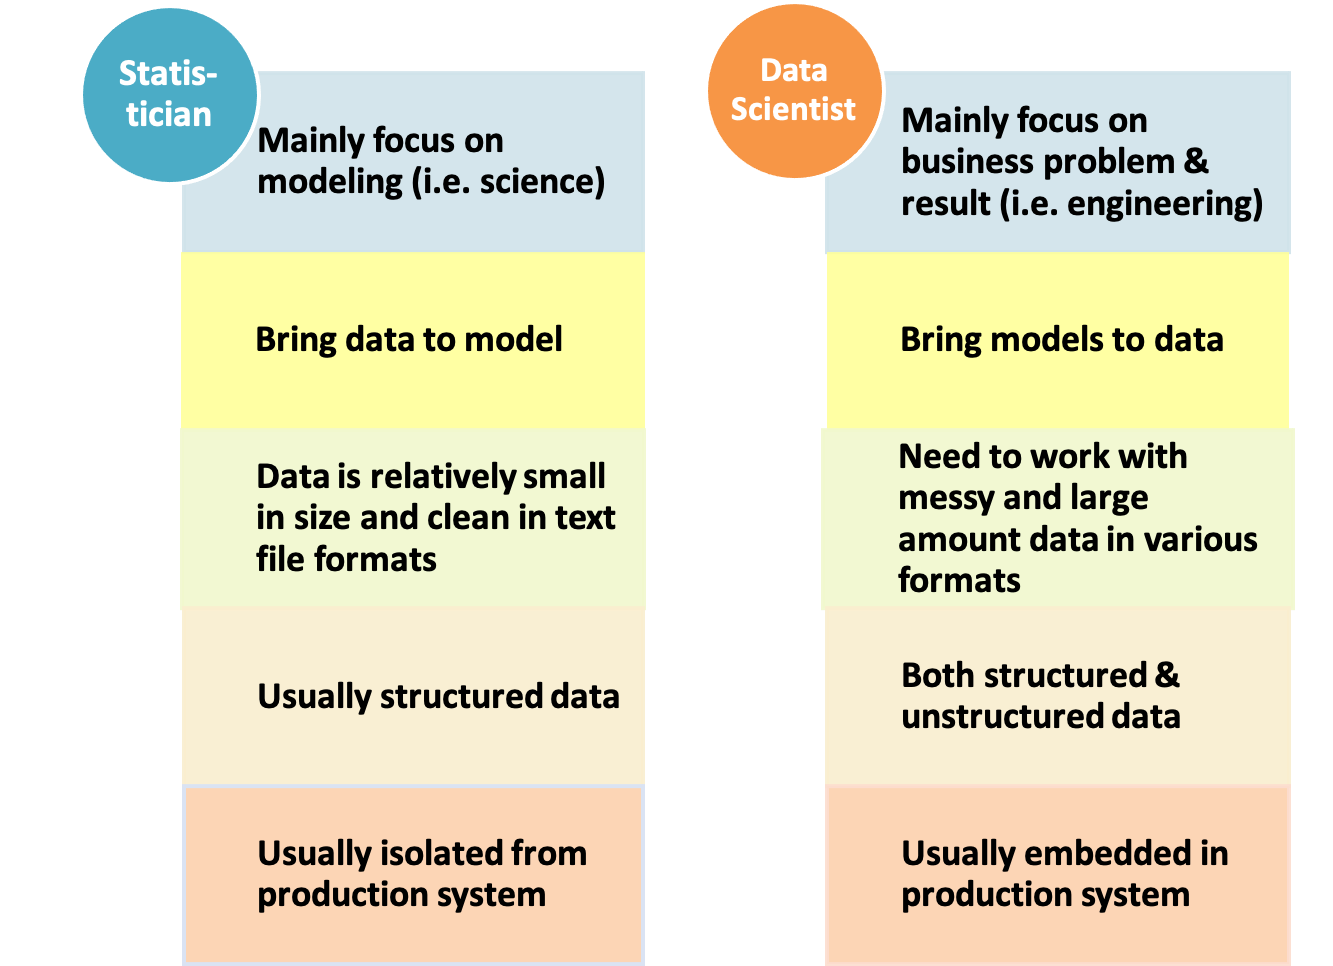
\includegraphics{images/softskill1.png}

Both statistician and data scientist work closely with data. For the
traditional statistician, the data is usually well-formatted text files
with numbers and labels. The size of the data usually can be fitted in a
PC's memory. Comparing to statisticians, data scientists need to deal
with more varieties of data:

\begin{itemize}
\tightlist
\item
  well-formatted data stored in a database system with size much larger
  than a PC's memory or hard-disk;
\item
  huge amount of verbatim text, voice, image, and video;
\item
  real-time streaming data and other types of records.
\end{itemize}

One unique power of statistics is to make statistical inference based on
a small set of data. Statisticians spend most of their time developing
models and don't need to put too much effort on data cleaning. Today,
data is relatively abundant, and modeling is only part of the overall
effort, often a small part. Due to the active development of some open
source communities, fitting models is not too far from button pushing.
Data scientists instead spend lot of time preprocessing and wrangling
the data before feeding them to the model.

Different from statisticians, data scientists often focus on delivering
actionable results and sometimes need to fit model on the cloud. The
data can be too large to read in laptop. From the entire problem-solving
cycle, statisticians are usually not well integrated with the production
system where data is obtained in real time; while data scientists are
more embedded in the production system and closer to the data generation
procedures.

\section{Beyond Data and Analytics}\label{beyond-data-and-analytics}

Data scientists usually have a good sense of data and analytics, but
data scientist project is more than that. A data science project may
involve people with different roles, especially in a big company:

\begin{itemize}
\tightlist
\item
  a business owner or leader to identify business value;
\item
  program manager to ensure the data science project fits into the
  overall technical program development and coordinate all parties to
  set periodical tasks so that the project meets the preset milestones
  and results;
\item
  data owner and computation resource and infrastructure owner from the
  IT department;
\item
  dedicated team to make sure the data and model are under model
  governance and privacy guidelines;
\item
  a team to implement, maintain and refresh the model;
\item
  multiple rounds of discussion of resource allocation among groups
  (i.e., who pay for the data science project).
\end{itemize}

Effective communication and in-depth domain knowledge about the business
problem are essential requirements for a successful data scientist. A
data scientist may interact with people at various levels from senior
leaders who set the corporate strategies to front-line employees who do
the daily work. A data scientist needs to have the capability to view
the problem from 10,000 feet above the ground, as well as down to the
detail to the very bottom. To convert a business question into a data
problem, a data scientist needs to communicate using the language the
other people can understand and obtain the required information.

In the entire process of data science project defining, planning,
executing and implementing, every step involves the data scientist to
ensure people correctly define the business problem and reasonably
evaluate the business value and success. Corporates are investing
heavily in data science and machine learning with a very high
expectation of return.

However, it is easy to set unrealistic goal and wrongly estimate the
business impact. The data scientist lead should navigate the discussions
to make sure the goal can be backed by data and analytics. Many data
science projects over promise and are too optimistic on the timeline.
These projects eventually fail by not delivering the preset business
impact within the timeline. As data scientists, we need to identify
these issues early in the stage and communicate with the entire team to
make sure the project has a realistic deliverable and timeline. The data
scientist team also need to work closely with data owners to identify
relevant internal and external data source and evaluate the quality of
the data; as well as working closely with the infrastructure team to
understand the computation resources (i.e.~hardware and software)
available for the data science project.

\section{Three Pillars of Knowledge}\label{three-pillars-of-knowledge}

\begin{enumerate}
\def\labelenumi{(\arabic{enumi})}
\tightlist
\item
  Analytics knowledge and tool sets
\end{enumerate}

A successful data scientist needs to have a strong technical background
in data mining, statistics and machine learning. The in-depth
understanding of modeling with the insight about data enable a data
scientist to convert a business problem to a data science problem.

\begin{enumerate}
\def\labelenumi{(\arabic{enumi})}
\setcounter{enumi}{1}
\tightlist
\item
  Domain knowledge and collaboration
\end{enumerate}

A successful data scientist needs some domain knowledge to understand
the business problem. For any data science project, the data scientist
need to collaborate with other team members and effective communication
and leadership skills are critical, especially when you are the only
data person in the room and you need to decide with uncertainty.

\begin{enumerate}
\def\labelenumi{(\arabic{enumi})}
\setcounter{enumi}{2}
\tightlist
\item
  (Big) data management and (new) IT skills
\end{enumerate}

The last pillar is about computation environment and model
implementation in a big data platform. This used to be the most
difficult one for a data scientist with statistics background (i.e.~lack
computer science or programming skills). The good news is that with the
rise of cloud computation big data platform, it is easier for a
statistician to overcome this barrier.

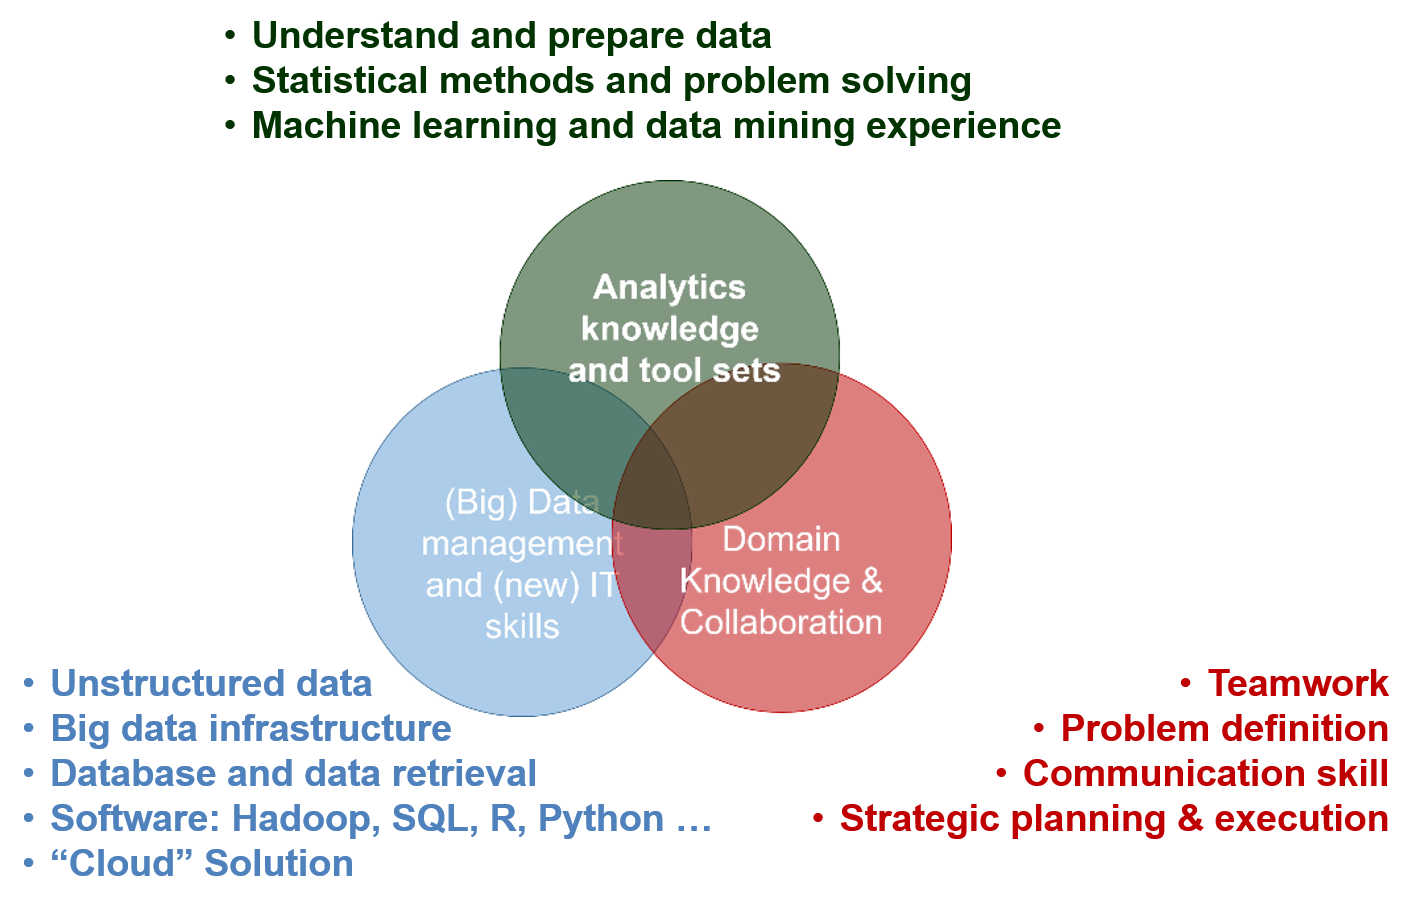
\includegraphics{images/softskill2.png}

\section{Data Science Project Cycle}\label{data-science-project-cycle}

A data science project has various stages. Many textbooks and blogs
focus on one or two specific stages and it is rare to see the end-to-end
life cycle of data science projects. In fact, to get a good grasp of the
end-to-end cycle requires many years of experience of doing real-world
data science. We will share our opinions on that in this section. Seeing
a holistic picture of the whole cycle helps you to better prepare for
real-world applications.

\subsection{Types of Data Science
Projects}\label{types-of-data-science-projects}

People often use data science project to describe any project that uses
data to solve a business problem, including traditional business
analytics or data visualization. Here we limit our discussion of data
science projects that involve data and some statistical or machine
learning models. The business problem itself gives us the flavor of the
project, data is the raw ingredient to start with, and the model makes
the dish. Different types of data science projects can be determined by
the types of data used and the final model development and
implementation.

\subsubsection{Offline and online Data}\label{offline-and-online-data}

There are offline and online data. Offline data are historical archived
data stored in databases or data warehouses. With the development of
data storage, the cost to store a large amount of data is cheap and
offline data are very rich in general (for example website may track and
store each individual user's mouse position, click and typing
information while the user is visiting the website). Offline data is
usually stored in a distributed system and it can be extracted in batch
as raw materials to create features that can be used in model training.
Online data are real-time information that can be feed to models to make
automatic actions. Real-time information can changes frequently such as
the keywords a customer is searching for. Capturing and using real-time
online data requires the integration of machine learning to the
production infrastructure. It used to be a steep learning curve for data
scientists, but the cloud infrastructure makes it much easier.

\subsubsection{Offline training and offline
application}\label{offline-training-and-offline-application}

This type of data science project is for a specific business problem
which needs to be solved once or multiple times. But the dynamic nature
of the business problem requires substantial work every time. One
example of such a project is ``whether a new workflow is going to
improve efficiency.'' In this situation, we often use offline internal
and external data, build models, and deliver the final results as a
report to answer the specific business question. It is similar to the
traditional business intelligence project but with more focus on data
and model. Sometimes the data size and model complexity are beyond the
capacity of a single computer. So you need to use distributed storage
and computation. Since the model is based on the historical data and the
output is a report, there is no need for real-time execution. Usually,
there is no run-time constraint on the machine learning model unless the
model is running beyond a reasonable time frame such as a few hours or a
few days. We can call this type of data science project
``offline~training, offline application'' project.

\subsubsection{Offline training and online
application}\label{offline-training-and-online-application}

Another type of data science project is to use offline data for training
and apply the trained model to real-time online data in the production
environment. One example of such a project is ``using historical data to
train a personalized advertisement model, and then provides real-time ad
recommendation when customers visit the website.'' The model is trained
based on offline data, and then use a customer's online real-time data
as features to run the model in real time to provide an automatic
action. The model training is very similar to the ``offline~training,
offline application'' project, but as the trained model will be put to
production, there are specific requirements such as features used in the
offline training have to be available online in real time, and the
online run-time of the model has to be short enough without impacting
user experience. In most cases, data science projects in this category
create continuous and scalable business value. We will use this type of
data science project to describe the project cycle.

\subsubsection{Online training and online
application}\label{online-training-and-online-application}

For some business problems, it is so dynamic that even yesterday's data
is out of date. For such cases, we can use online data to train the
model and then applying it in real time. We call this type of data
science project ``online~training, online application.'' This type of
data science project requires high automation and low latency.

\subsection{At the Planning Stage}\label{at-the-planning-stage}

To ensure a successful data science project, a data-driven and
fact-based planning stage is essential. With the recent big data and
data science hype, there is a high demand for data science projects to
create business value across different business sectors. Often times,
these data science project proposals are initiated by the leaders of an
organization. This top-down style data science projects usually have
high visibility with certain human and computation resources
pre-allocated. However, it is crucial to understand the business problem
first and align the goal across different teams including

\begin{enumerate}
\def\labelenumi{(\arabic{enumi})}
\item
  the business team which may include members from the business
  operation team, business analyst, insight and reporting team;
\item
  technology team which may include members from database and data
  warehouse team, data engineering team, infrastructure team, core
  machine learning team, and software development team; (3) project
  management team which may include program management team and product
  management team depending on the scope of the data science project.
\end{enumerate}

To start the conversation, we can ask the following questions to
everyone in the team:

\begin{itemize}
\tightlist
\item
  What are the pain points in current business operation?
\item
  What data are available and how is the quality and quantity of the
  data?
\item
  What might be the most significant impacts of a data science project?
\item
  Are there any negative impact to other teams?
\item
  What computation resources are available for model training and model
  execution?
\item
  Can we define key metrics to compare and quantity business value?
\item
  Are there any data security, privacy and legal concerns?
\item
  What are the desired milestones, check points and timeline?
\item
  Is the final application online or offline?
\item
  Are the data online or offline?
\end{itemize}

It is likely to have a series of intense meetings and heated discussions
to frame the project to a reasonable scope. After the planning stage, we
should be able to define a set of key metrics related to the project,
identify some offline and online data sources, request needed
computation resources, draft tentative timeline and milestones, and form
a team of data scientist, data engineer, software developer, project
manager and members from business operation. Data scientists should play
a major role in these discussions. If data scientist is not leading the
data science project formulation, it is very likely the entire project
will not reach the timeline and milestones.

\subsection{At the Modeling Stage}\label{at-the-modeling-stage}

Even though at the planning stage we already set some strategy,
milestone, and timeline, data science projects are dynamic in nature and
there could be uncertainties along the road. As a data scientist,
clearly communicate any newly encountered difficulties during the
modeling stage to the entire team is essential to keep the data science
project progress. With the available data source identified at the
planning stage, data clearing, data wrangling, and exploratory data
analysis are great starting points toward modeling. Meanwhile,
abstracting the business problem to be a set of statistical and machine
learning problems is an iterative process. It is rare that business
problems can be solved by using just one statistical or machine learning
model. The ability to use a sequence of methods to decompose the
business problem is one of the key responsibility for a senior data
scientist. The process requires iterative rounds of discussions with the
business team and data engineering team based on the new learning from
each iteration. Each iteration includes both data related and model
related part.

\subsubsection{Data related}\label{data-related}

Data cleaning, data preprocessing and feature engineering are closely
related procedures. The goal of these data-related procedures is to
create usable variables or features for statistical and machine learning
models. One important aspect of data related procedures is to make sure
the data source we are using is a good representation of the situation
where the final trained model will be applied. The exact same
representation is rarely possible, and reasonable approximation is
totally fine to start with. A data scientist has to be clear on the
assumptions and communicate with the entire team the limitations of
biased data and quantify its impact on the application. In data related
part, sometimes the available data is not that relevant to the business
problem we want to solve, and we have to collect more data.

\subsubsection{Model related}\label{model-related}

There are different types of statistical and machine learning models,
such as supervised learning, unsupervised learning, and causal
inference. For each type, there are various algorithms, libraries, or
packages readily available. To solve a business problem, you sometimes
need to piece together a few methods at the model exploring and
developing stage. This stage also includes model training, validation,
and testing to make sure the model works well in the production
environment; i.e., it is not overfitting and can be generalized.~The
model selection follows Occam's razor, which is to choose the simplest
among a set of compatible models. Before you try complicated models, it
is a good practice to get some benchmark by additional business rules,
common sense decision, or standard models (such as random forest for
classification).

\subsection{At the Production Stage}\label{at-the-production-stage}

For offline application data science projects, the end product is often
a detailed report with model result and output. However, for online
application projects, a trained model is just halfway from the finish
line. The offline data is stored and processed in a totally different
environment from the online production environment. Building the online
data pipeline and implementing machine learning models in a production
environment requires lots of additional work. Even though recent advance
in cloud infrastructure lowers the barrier dramatically, it still takes
effort to implement an offline model in the online production system.
Before you promote the model to production, there are two more steps to
go:

\begin{enumerate}
\def\labelenumi{\arabic{enumi}.}
\tightlist
\item
  shadow mode
\item
  A/B testing
\end{enumerate}

A \textbf{shadow mode} is like an observation period when the data
pipeline and machine learning models run as it is fully functional, but
we only record the model output without any actions. Some people call it
proof of concept (POC). During POC, people frequently check the data
pipeline and model and detect bugs such as a timeout or missing
features, version conflict (for example python 2 v.s. python 3), data
type mismatch, etc.

Once the online model passes the shadow mode, \textbf{A/B testing} is
the next stage. During A/B testing, all the incoming observations are
randomly separated into two groups: control and treatment. The control
group is going to skip the machine learning model, while the treatment
group is going through the machine learning model. After that, people
monitor a list of pre-defined key metrics during a specific time period
to compare the control and treatment groups. The differences in these
key metrics determine whether the machine learning model provides
business value or not. Real applications can be complicated. For
example, there can be multiple treatment groups, or hundreds, even
thousands of A/B testing running by different teams at any given time.

Once the A/B testing shows that the model provides significant business
value, then you can put it into full production. It is ideal that the
model runs as expected and continues to provide scalable values.
However, the business can change and a machine learning model works now
can break tomorrow, and features available now may not be available
tomorrow. You need a monitoring system to automatically notify us when
one or multiple features change. When the model performance degrades
below a pre-defined a level, you need to fine-tune the parameters and
thresholds, re-train the model with more recent data, add or remove
features to improve model performance. Eventually, any model will fail
or retire at some time.

\subsection{Summary}\label{summary}

Data science end-to-end project cycle is a complicated process which
requires close collaboration among many teams. Data scientist, maybe the
only scientist in the team, has to lead the planning discussion and
model development based on data available and clearly communicate key
assumptions and uncertainties with the entire team. A data science
project may fail at any stage, and a clear end-to-end cycle view of the
project helps avoid some mistakes.

\section{Common Mistakes in Data
Science}\label{common-mistakes-in-data-science}

Data science project can go wrong at different stages in many ways. Most
textbooks and online blogs~focus on technical mistakes about machine
learning model, algorithm or theory, such as including outliers and
overfitting. It is important to avoid these technical mistakes. However,
there are common systematic mistakes across data science projects that
are rarely discussed in textbooks. To summarize these mistakes, people
need to do real-world data science projects. In this section, we
describe these common mistakes in detail so that readers can proactively
identify and avoid these systematic mistakes in their own data science
projects.

\subsection{Problem Formulation Stage}\label{problem-formulation-stage}

The most challenging part of a data science project is problem
formulation. Data science project stems from pain points of the
business. The draft version of the goal of the project is relatively
vague without much quantification or is the gut feeling of the
leadership team. Often there are multiple teams involved in the initial
project formulation stage and they have different views. It is easy to
have malalignment across different teams such as resource allocation,
milestone deliverable, and timeline. At the problem formulation stage,
data science team members with technical background sometimes are not
even invited to the initial discussion. It sounds ridiculous, but sadly
true that a lot of resources are spent on \textbf{solving the wrong
problem,} the number one systematic common mistake in data science.
Formulating a business problem into the right data science project
requires an in-depth understanding of the business context, data
availability and quality, computation infrastructure, and methodology to
leverage the data to quantify business value.

We have seen people over promise about business value all the time,
another common mistake that is going to fail the project at the
beginning. With the hype of big data and machine learning, leaders
across industries often have unrealistic high expectation on data
science. It is especially true during enterprise transformation when
there is a strong push to adopt new technology to get value out of the
data. The unrealistic expectations are based on assumptions that are way
off chart without checking~the data availability, data quality,
computation resource, and current best practices in the field.~Even
there is some exploratory analysis by the data science team at the
problem formulation stage,~project leaders sometimes ignore their
data-driven voice.

These two systematic mistakes undermine the organization's data science
strategy.~The higher the expectation, the bigger the disappointment when
the project cannot deliver business value. Data and business context are
essential to formulate the business problem and set reachable business
value. It helps to avoid the mistakes by having a strong data science
leader with a broad technical background and let data scientist
coordinate and drive the problem formulation and set realistic goals
based data and business context.

\subsection{Problem Planning Stage}\label{problem-planning-stage}

Now suppose the data science project is formulated correctly with a
reasonable expectation on the business value. The next step is to plan
the project such as allocating resources, setting up milestones and
timeline, and defining deliverable. In most cases, there are project
managers to coordinate different teams that are involved in the project
and use agile project management tools similar to those in software
development. Unfortunately,~the project management team may not have
experience with data science projects and hence fail to account for the
uncertainties at the planning stage. The fundamental difference between
data science projects and other projects lead to another common mistake:
\textbf{too optimistic about the timeline}. For example, data
exploratory and preparation may take 60\% to 80\% of the total time for
a given data science project, but people often don't realize that.

When there are lots of data already collected across the organization,
people assume you have enough data for everything. It leads to the
mistake: t\textbf{oo optimistic about data availability and quality}.
What you need is not ``big data'', but data that can help you solve the
problem. The data available may be low quality and you need to put
substantial efforts to clean the data before you can use it. There are
``unexpected'' efforts to bring the right and relevant data for a
specific data science project. To ensure smooth delivery of data science
projects, you need to account for the ``unexpected'' work at the
planning stage. We all know data pre-processing and feature engineering
is usually the most time-consuming part of a data science project.
However, people outside data science are not aware of it and we need to
educate other team members and the leadership team.

\subsection{Modeling Stage}\label{modeling-stage}

Finally, you start to look at the data and fit some models. One common
mistake at this stage is unrepresentative data. The model trained using
historical data may not generalize to the future. There is always a
problem of biased or unrepresentative data. As a data scientist, we need
to use data that are closer to the situation where the model is going to
apply and quantify the impact of model output in production. Another
mistake at this stage is overfitting and obsession for complicated
models. Now we can easily get hundreds or even thousands of features and
the machine learning models are getting more complicated. People can use
open source libraries to try all kinds of models. People are sometimes
obsessed with complicated models instead of using the simplest among a
set of compatible models.

The data used to build the models is always biased or unrepresentative
to some extent, simpler models are better to generalize and it has a
higher chance to provide consistent business value once the model passes
the test and is finally implemented in the production environment. It is
possible that you can not use the existing data and methods to solve the
business problem. You can try to collect more data, do feature
engineering, or create your own models. However, if there is a
fundamental gap between data and the business problem, the data
scientist has to make the tough decision to unplug the project. On the
other hand, data science projects usually have high visibility and may
be initiated by senior leadership. Even the data science team provide
enough evidence that they can't deliver the expected business
value,~people may not want to stop the project which leads another
common mistake at modeling stage: \textbf{take too long to fail}. The
earlier we can stop a failing project, the better. Because we can put
valuable resources to other promising projects. It damages the data
science strategy and everyone will be hurt by a long data science
project that is doomed to fail.

\subsection{Production Stage}\label{production-stage}

Now suppose you have found a model that works great for the training and
testing data. If it is an online application, you are halfway. The next
is to put the model in production, which sounds like alien work for a
data scientist. It is true that the data engineering team can help with
model production. However, as a data scientist, you need to know the
potential mistakes at this stage. One big mistake is \textbf{missing A/B
testing} and assuming that the model performance at model
training/testing stays the same in the production environment.
Unfortunately, the model trained and evaluated using historical data
nearly never performs the same in the production environment. The data
used in the offline training maybe significant different from online
data and the business context may have changed. If possible, machine
learning models in production should always go through A/B testing to
evaluate performance.

In the model training stage, people usually focus on model performance,
such as accuracy without paying too much attention to the model
execution time. When a model runs online in real time, the total run
time for each instance (i.e., model latency) should not impact the
customer's user experience. Nobody wants to wait for even one second to
see the results after click the ``Search'' button. In the production
stage, feature availability is crucial to run a real-time
model.~Engineering resources are essential for model production.
However, in traditional companies, it is common that a data science
project \textbf{fail to scale in real time applications} due to lack of
computation capacity, engineering resources, or non-tech culture and
environment.

As the business problem evolve rapidly, the data and model in the
production environment need to change accordingly or the performance of
the model deteriorates over time. The online production environment is
more complicated than model training and testing, for example, you pull
online features from different resources, and some features may be
missing at a specific time; the model may run into time out zone, and
there are tons of different software and data exceptions that may
happen. We need regular checkup during the entire life of the model
cycle from implementation to retirement. Unfortunately, people often
don't set the monitoring system for data science projects, and it is
another common mistake: \textbf{missing necessary online checkup}. It is
essential to set a monitoring dashboard and automatic alarms, create
model tuning, re-training, and retirement plans.

\subsection{Summary}\label{summary-1}

The data science project is a combination of art and engineering. A data
science project may fail in different ways. However, if we put data and
business context at the center of the project, get familiar with the
data science project cycle and proactively identify and avoid these
potential mistakes, the data science project can provide significant
business value. Here is the summary of the mistakes:

\begin{itemize}
\tightlist
\item
  Solving the wrong problem
\item
  Over promise on business value
\item
  Too optimistic about the timeline
\item
  Too optimistic about data availability and quality
\item
  Unrepresentative data
\item
  Overfitting and obsession for complicated models
\item
  Take too long to fail
\item
  Missing A/B testing
\item
  Fail to scale in real-time applications
\item
  Missing necessary online checkup
\end{itemize}

\chapter{Introduction to the data}\label{introduction-to-the-data}

Before tackling analytics problem, we start by introducing data to be
analyzed in later chapters.

\section{Customer Data for Clothing
Company}\label{customer-data-for-clothing-company}

Our first data set represents customers of a clothing company who sells
products in physical stores and online. This data is typical of what one
might get from a company's marketing data base (the data base will have
more data than the one we show here). This data includes 1000 customers:

\begin{enumerate}
\def\labelenumi{\arabic{enumi}.}
\tightlist
\item
  Demography

  \begin{itemize}
  \tightlist
  \item
    \texttt{age}: age of the respondent
  \item
    \texttt{gender}: male/female
  \item
    \texttt{house}: 0/1 variable indicating if the customer owns a house
    or not
  \end{itemize}
\item
  Sales in the past year

  \begin{itemize}
  \tightlist
  \item
    \texttt{store\_exp}: expense in store
  \item
    \texttt{online\_exp}: expense online
  \item
    \texttt{store\_trans}: times of store purchase
  \item
    \texttt{online\_trans}: times of online purchase
  \end{itemize}
\item
  Survey on product preference
\end{enumerate}

It is common for companies to survey their customers and draw insights
to guide future marketing activities. The survey is as below:

How strongly do you agree or disagree with the following statements:

\begin{enumerate}
\def\labelenumi{\arabic{enumi}.}
\tightlist
\item
  Strong disagree
\item
  Disagree
\item
  Neither agree nor disagree
\item
  Agree
\item
  Strongly agree
\end{enumerate}

\begin{itemize}
\tightlist
\item
  Q1. I like to buy clothes from different brands
\item
  Q2. I buy almost all my clothes from some of my favorite brands
\item
  Q3. I like to buy premium brands
\item
  Q4. Quality is the most important factor in my purchasing decision
\item
  Q5. Style is the most important factor in my purchasing decision
\item
  Q6. I prefer to buy clothes in store
\item
  Q7. I prefer to buy clothes online
\item
  Q8. Price is important
\item
  Q9. I like to try different styles
\item
  Q10. I like to make decision myself and don't need too much of others'
  suggestions
\end{itemize}

There are 4 segments of customers:

\begin{enumerate}
\def\labelenumi{\arabic{enumi}.}
\tightlist
\item
  Price
\item
  Conspicuous
\item
  Quality
\item
  Style
\end{enumerate}

Let's check it:

\begin{Shaded}
\begin{Highlighting}[]
\KeywordTok{str}\NormalTok{(sim.dat,}\DataTypeTok{vec.len=}\DecValTok{3}\NormalTok{)}
\end{Highlighting}
\end{Shaded}

\begin{verbatim}
## 'data.frame':    1000 obs. of  19 variables:
##  $ age         : int  57 63 59 60 51 59 57 57 ...
##  $ gender      : Factor w/ 2 levels "Female","Male": 1 1 2 2 2 2 2 2 ...
##  $ income      : num  120963 122008 114202 113616 ...
##  $ house       : Factor w/ 2 levels "No","Yes": 2 2 2 2 2 2 2 2 ...
##  $ store_exp   : num  529 478 491 348 ...
##  $ online_exp  : num  304 110 279 142 ...
##  $ store_trans : int  2 4 7 10 4 4 5 11 ...
##  $ online_trans: int  2 2 2 2 4 5 3 5 ...
##  $ Q1          : int  4 4 5 5 4 4 4 5 ...
##  $ Q2          : int  2 1 2 2 1 2 1 2 ...
##  $ Q3          : int  1 1 1 1 1 1 1 1 ...
##  $ Q4          : int  2 2 2 3 3 2 2 3 ...
##  $ Q5          : int  1 1 1 1 1 1 1 1 ...
##  $ Q6          : int  4 4 4 4 4 4 4 4 ...
##  $ Q7          : int  1 1 1 1 1 1 1 1 ...
##  $ Q8          : int  4 4 4 4 4 4 4 4 ...
##  $ Q9          : int  2 1 1 2 2 1 1 2 ...
##  $ Q10         : int  4 4 4 4 4 4 4 4 ...
##  $ segment     : Factor w/ 4 levels "Conspicuous",..: 2 2 2 2 2 2 2 2 ...
\end{verbatim}

Refer to Appendix for the simulation code.

\section{Customer Satisfaction Survey Data from Airline
Company}\label{customer-satisfaction-survey-data-from-airline-company}

This data set is from a customer satisfaction survey for three airline
companies. There are \texttt{N=1000} respondents and 15 questions. The
market researcher asked respondents to recall the experience with
different airline companies and assign a score (1-9) to each airline
company for all the 15 questions. The higher the score, the more
satisfied the customer to the specific item. The 15 questions are of 4
types (the variable names are in the parentheses):

\begin{itemize}
\tightlist
\item
  How satisfied are you with our\_\_\_\_\_\_?
\end{itemize}

\begin{enumerate}
\def\labelenumi{\arabic{enumi}.}
\tightlist
\item
  Ticketing

  \begin{itemize}
  \tightlist
  \item
    Ease of making reservation(Easy\_Reservation)
  \item
    Availability of preferred seats(Preferred\_Seats)
  \item
    Variety of flight options(Flight\_Options)
  \item
    Ticket prices(Ticket\_Prices)
  \end{itemize}
\item
  Aircraft

  \begin{itemize}
  \tightlist
  \item
    Seat comfort(Seat\_Comfort)
  \item
    Roominess of seat area(Seat\_Roominess)
  \item
    Availability of Overhead(Overhead\_Storage)
  \item
    Cleanliness of aircraft(Clean\_Aircraft)
  \end{itemize}
\item
  Service

  \begin{itemize}
  \tightlist
  \item
    Courtesy of flight attendant(Courtesy)
  \item
    Friendliness(Friendliness)
  \item
    Helpfulness(Helpfulness)
  \item
    Food and drinks(Service)
  \end{itemize}
\item
  General

  \begin{itemize}
  \tightlist
  \item
    Overall satisfaction(Satisfaction)
  \item
    Purchase again(Fly\_Again)
  \item
    Willingness to recommend(Recommend)
  \end{itemize}
\end{enumerate}

Now check the data frame we have:

\begin{Shaded}
\begin{Highlighting}[]
\KeywordTok{str}\NormalTok{(rating,}\DataTypeTok{vec.len=}\DecValTok{3}\NormalTok{)}
\end{Highlighting}
\end{Shaded}

\begin{verbatim}
## 'data.frame':    3000 obs. of  17 variables:
##  $ Easy_Reservation: int  6 5 6 5 4 5 6 4 ...
##  $ Preferred_Seats : int  5 7 6 6 5 6 6 6 ...
##  $ Flight_Options  : int  4 7 5 5 3 4 6 3 ...
##  $ Ticket_Prices   : int  5 6 6 5 6 5 5 5 ...
##  $ Seat_Comfort    : int  5 6 7 7 6 6 6 4 ...
##  $ Seat_Roominess  : int  7 8 6 8 7 8 6 5 ...
##  $ Overhead_Storage: int  5 5 7 6 5 4 4 4 ...
##  $ Clean_Aircraft  : int  7 6 7 7 7 7 6 4 ...
##  $ Courtesy        : int  5 6 6 4 2 5 5 4 ...
##  $ Friendliness    : int  4 6 6 6 3 4 5 5 ...
##  $ Helpfulness     : int  6 5 6 4 4 5 5 4 ...
##  $ Service         : int  6 5 6 5 3 5 5 5 ...
##  $ Satisfaction    : int  6 7 7 5 4 6 5 5 ...
##  $ Fly_Again       : int  6 6 6 7 4 5 3 4 ...
##  $ Recommend       : int  3 6 5 5 4 5 6 5 ...
##  $ ID              : int  1 2 3 4 5 6 7 8 ...
##  $ Airline         : Factor w/ 3 levels "AirlineCo.1",..: 1 1 1 1 1 1 1 1 ...
\end{verbatim}

Refer to Appendix for the simulation code.

\section{Swine Disease Breakout Data}\label{swine-disease-breakout-data}

The swine disease data includes simulated 120 survey questions from 800
farms. There are three choices for each question. The outbreak status
for the \(i^{th}\) farm is generated from a \(Bernoulli(1, p_i)\)
distribution with \(p_i\) being a function of the question answers:

\[ln(\frac{p_i}{1-p_i})=\beta_0 + \Sigma_{g=1}^G\mathbf{x_{i,g}^T\beta_{g}}\]

where \(\beta_0\) is the intercept, \(\mathbf{x_{i,g}}\) is a
three-dimensional indication vector for question answer and
\(\mathbf(\beta_g)\) is the parameter vector corresponding to the
\(g^{th}\) predictor. Three types of questions are considered regarding
their effects on the outcome. The first forty survey questions are
important questions such that the coefficients of the three answers to
these questions are all different:

\[\mathbf{\beta_g}=(1,0,-1)\times \gamma,\ g=1,\dots,40\]

The second forty survey questions are also important questions but only
one answer has a coefficient that is different from the other two
answers:

\[\mathbf{\beta_g}=(1,0,0)\times \gamma,\ g=41,\dots,80\]

The last forty survey questions are also unimportant questions such that
all three answers have the same coefficients:

\[\mathbf{\beta_g}=(0,0,0)\times \gamma,\ g=81,\dots,120\]

The baseline coefficient \(\beta_0\) is set to be
\(-\frac{40}{3}\gamma\) so that on average a farm have 50\% of chance to
have an outbreak. The parameter \(\gamma\) in the above simulation is
set to control the strength of the questions' effect on the outcome. In
this simulation study, we consider the situations where
\(\gamma = 0.1, 0.25, 0.5, 1, 2\). So the parameter settings are:

\[\mathbf{\beta^{T}}=\left(\underset{question\ 1}{\frac{40}{3},\underbrace{1,0,-1}},...,\underset{question\ 40}{\underbrace{1,0,-1}},\underset{question\ 41}{\underbrace{1,0,0}},...,\underset{question\ 80}{\underbrace{1,0,0}},\underset{question\ 81}{\underbrace{0,0,0}},...,\underset{question\ 120}{\underbrace{0,0,0}}\right)*\gamma\]

For each value of \(\gamma\), 20 data sets are simulated. The bigger
\(\gamma\) is, the larger the corresponding parameter. We provided the
data sets with \(\gamma = 2\). Let's check the data:

\begin{Shaded}
\begin{Highlighting}[]
\NormalTok{disease_dat<-}\KeywordTok{read.csv}\NormalTok{(}\StringTok{"http://bit.ly/2KXb1Qi"}\NormalTok{)}
\CommentTok{# only show the last 7 columns here}
\KeywordTok{head}\NormalTok{(}\KeywordTok{subset}\NormalTok{(disease_dat,}\DataTypeTok{select=}\KeywordTok{c}\NormalTok{(}\StringTok{"Q118.A"}\NormalTok{,}\StringTok{"Q118.B"}\NormalTok{,}\StringTok{"Q119.A"}\NormalTok{,}
                                 \StringTok{"Q119.B"}\NormalTok{,}\StringTok{"Q120.A"}\NormalTok{,}\StringTok{"Q120.B"}\NormalTok{,}\StringTok{"y"}\NormalTok{))) }
\end{Highlighting}
\end{Shaded}

\begin{verbatim}
##   Q118.A Q118.B Q119.A Q119.B Q120.A Q120.B y
## 1      1      0      0      0      0      1 1
## 2      0      1      0      1      0      0 1
## 3      1      0      0      0      1      0 1
## 4      1      0      0      0      0      1 1
## 5      1      0      0      0      1      0 0
## 6      1      0      0      1      1      0 1
\end{verbatim}

Here \texttt{y} indicates the outbreak situation of the farms.
\texttt{y=1} means there is an outbreak in 5 years after the survey. The
rest columns indicate survey responses. For example
\texttt{Q120.A\ =\ 1} means the respondent chose \texttt{A} in Q120. We
consider \texttt{C} as the baseline.

Refer to Appendix for the simulation code.

\section{MNIST Dataset}\label{mnist-dataset}

The MNIST dataset is a popular dataset for image classification machine
learning model tutorials. It is conveniently included in the Keras
library and ready to be loaded with build-in functions for analysis. The
WIKI page of MNIST provides a detailed description of the dataset:
\url{https://en.wikipedia.org/wiki/MNIST_database}. It contains 70,000
images of handwritten digits from American Census Bureau employees and
American high school students. There are 60,000 training images and
10,000 testing images. Each image has a resolution of 28x28, and the
numerical pixel values are in greyscale. Each image is represented by a
28x28 matrix with each element of the matrix an integer between 0 and
255. The label of each image is the intended digit of the handwritten
image between 0 and 9. We cover the detailed steps to explore the MNIST
dataset in the R and Python notebooks. A sample of the dataset is
illustrated in the figure below:

\begin{figure}
\centering
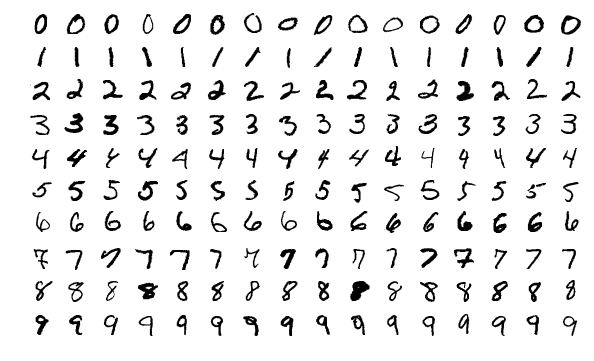
\includegraphics[width=0.70000\textwidth]{images/MnistExamples.png}
\caption{Sample of MNIST dataset
(\url{https://en.wikipedia.org/wiki/File:MnistExamples.png})}
\end{figure}

\section{IMDB Dataset}\label{imdb-dataset}

The IMDB dataset (\url{http://ai.stanford.edu/~amaas/data/sentiment/})
is a popular dataset for text and language-related machine learning
tutorials. It is also conveniently included in the Keras library, and
there are a few build-in functions in Keras for data loading and
pre-processing. It contains 50,000 movie reviews (25,000 in training and
25,000 in testing) from IMDB, as well as each movie review's binary
sentiment: positive or negative. The raw data contains the text of each
movie review, and it has to be pre-processed before being fitted with
any machine learning models. By using Keras's built-in functions, we can
easily get the processed dataset (i.e., a numerical data frame) for
machine learning algorithms. Keras' build-in functions perform the
following tasks to convert the raw review text into a data frame:

\begin{enumerate}
\def\labelenumi{\arabic{enumi}.}
\tightlist
\item
  Convert text data into numerical data. Machine learning models cannot
  work with raw text data directly, and we have to convert text into
  numbers. There are many different ways for the conversion and Keras'
  build-in function uses each word's rank of frequency in the entire
  training dataset to replace the raw text in both the training and
  testing dataset. For example, the 10th most frequent word is replaced
  by integer 10. There are a few additional setups for this process,
  including:~

  \begin{enumerate}
  \def\labelenumii{\alph{enumii}.}
  \tightlist
  \item
    Skip top frequent words. We usually skip a few top frequent words as
    they are mainly stopwords like ``the'' ``and'' or ``a,'' which
    usually do not provide much information. There is a parameter in the
    build-in function to specify how many top words to skip.\\
  \item
    Set the maximum number of unique words. The entire vocabulary of the
    unique words in the training dataset may be large, and many of them
    have very low frequencies such as just appearing once in the entire
    training dataset.~To keep the size of the vocabulary, we can also
    set up the maximum number of the unique words using Keras' built-in
    function such that any words with least frequencies will be replaced
    with a special index such as ``2''.~
  \end{enumerate}
\item
  Padding or truncation to keep all the reviews to be the same length.
  For most machine learning models, the algorithms expect to see the
  same number of features (i.e., same number of input columns in the
  data frame). There is a parameter in the Keras build-in function to
  set the maximum number of words in each review (i.e., max\_length).
  For reviews that have less than max\_legth words, we pad them with
  ``0''. For reviews that have more than max\_length words, we truncate
  them.~
\end{enumerate}

After the above pre-processing, each review is represented by one row in
the data frame. There is one column for the binary positive/negative
sentiment, and max\_length columns input features converted from the raw
review text. In the corresponding R and Python notebooks, we will go
over the details of the data pre-processing using Keras' built-in
functions.

\chapter{Data Pre-processing}\label{data-pre-processing}

Many data analysis related books focus on models, algorithms and
statistical inferences. However, in practice, raw data is usually not
directly used for modeling. Data preprocessing is the process of
converting raw data into clean data that is proper for modeling. A model
fails for various reasons. One is that the modeler doesn't correctly
preprocess data before modeling. Data preprocessing can significantly
impact model results, such as imputing missing value and handling with
outliers. So data preprocessing is a very critical part.

\begin{figure}
\centering
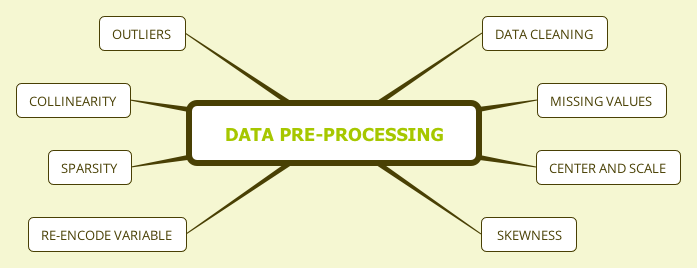
\includegraphics[width=0.90000\textwidth]{images/DataPre-processing.png}
\caption{Data Pre-processing Outline}
\end{figure}

In real life, depending on the stage of data cleanup, data has the
following types:

\begin{enumerate}
\def\labelenumi{\arabic{enumi}.}
\tightlist
\item
  Raw data
\item
  Technically correct data
\item
  Data that is proper for the model
\item
  Summarized data
\item
  Data with fixed format
\end{enumerate}

The raw data is the first-hand data that analysts pull from the
database, market survey responds from your clients, the experimental
results collected by the R \& D department, and so on. These data may be
very rough, and R sometimes can't read them directly. The table title
could be multi-line, or the format does not meet the requirements:

\begin{itemize}
\tightlist
\item
  Use 50\% to represent the percentage rather than 0.5, so R will read
  it as a character;
\item
  The missing value of the sales is represented by ``-'' instead of
  space so that R will treat the variable as character or factor type;
\item
  The data is in a slideshow document, or the spreadsheet is not
  ``.csv'' but ``.xlsx''
\item
  \ldots{}
\end{itemize}

Most of the time, you need to clean the data so that R can import them.
Some data format requires a specific package. Technically correct data
is the data, after preliminary cleaning or format conversion, that R (or
another tool you use) can successfully import it.

Assume we have loaded the data into R with reasonable column names,
variable format and so on. That does not mean the data is entirely
correct. There may be some observations that do not make sense, such as
age is negative, the discount percentage is greater than 1, or data is
missing. Depending on the situation, there may be a variety of problems
with the data. It is necessary to clean the data before modeling.
Moreover, different models have different requirements on the data. For
example, some model may require the variables are of consistent scale;
some may be susceptible to outliers or collinearity, some may not be
able to handle categorical variables and so on. The modeler has to
preprocess the data to make it proper for the specific model.

Sometimes we need to aggregate the data. For example, add up the daily
sales to get annual sales of a product at different locations. In
customer segmentation, it is common practice to build a profile for each
segment. It requires calculating some statistics such as average age,
average income, age standard deviation, etc. Data aggregation is also
necessary for presentation, or for data visualization.

The final table results for clients need to be in a nicer format than
what used in the analysis. Usually, data analysts will take the results
from data scientists and adjust the format, such as labels, cell color,
highlight. It is important for a data scientist to make sure the results
look consistent which makes the next step easier for data analysts.

It is highly recommended to store each step of the data and the R code,
making the whole process as repeatable as possible. The R markdown
reproducible report will be extremely helpful for that. If the data
changes, it is easy to rerun the process. In the remainder of this
chapter, we will show the most common data preprocessing methods.

Load the R packages first:

\begin{Shaded}
\begin{Highlighting}[]
\CommentTok{# install packages from CRAN}
\NormalTok{p_needed <-}\StringTok{ }\KeywordTok{c}\NormalTok{(}\StringTok{'imputeMissings'}\NormalTok{,}\StringTok{'caret'}\NormalTok{,}\StringTok{'e1071'}\NormalTok{,}\StringTok{'psych'}\NormalTok{,}\StringTok{'car'}\NormalTok{,}\StringTok{'corrplot'}\NormalTok{)}
\NormalTok{packages <-}\StringTok{ }\KeywordTok{rownames}\NormalTok{(}\KeywordTok{installed.packages}\NormalTok{())}
\NormalTok{p_to_install <-}\StringTok{ }\NormalTok{p_needed[}\OperatorTok{!}\NormalTok{(p_needed }\OperatorTok\StringTok{ }\NormalTok{packages)]}
\ControlFlowTok{if}\NormalTok{ (}\KeywordTok{length}\NormalTok{(p_to_install) }\OperatorTok{>}\StringTok{ }\DecValTok{0}\NormalTok{) \{}
    \KeywordTok{install.packages}\NormalTok{(p_to_install)}
\NormalTok{\}}

\KeywordTok{lapply}\NormalTok{(p_needed, require, }\DataTypeTok{character.only =} \OtherTok{TRUE}\NormalTok{)}
\end{Highlighting}
\end{Shaded}

\section{Data Cleaning}\label{data-cleaning}

After you load the data, the first thing is to check how many variables
are there, the type of variables, the distributions, and data errors.
Let's read and check the data:

\begin{Shaded}
\begin{Highlighting}[]
\NormalTok{sim.dat <-}\StringTok{ }\KeywordTok{read.csv}\NormalTok{(}\StringTok{"http://bit.ly/2P5gTw4"}\NormalTok{)}
\KeywordTok{summary}\NormalTok{(sim.dat)}
\end{Highlighting}
\end{Shaded}

\begin{verbatim}
      age           gender        income       house       store_exp    
 Min.   : 16.0   Female:554   Min.   : 41776   No :432   Min.   : -500  
 1st Qu.: 25.0   Male  :446   1st Qu.: 85832   Yes:568   1st Qu.:  205  
 Median : 36.0                Median : 93869             Median :  329  
 Mean   : 38.8                Mean   :113543             Mean   : 1357  
 3rd Qu.: 53.0                3rd Qu.:124572             3rd Qu.:  597  
 Max.   :300.0                Max.   :319704             Max.   :50000  
                              NA's   :184                               
   online_exp    store_trans     online_trans        Q1            Q2      
 Min.   :  69   Min.   : 1.00   Min.   : 1.0   Min.   :1.0   Min.   :1.00  
 1st Qu.: 420   1st Qu.: 3.00   1st Qu.: 6.0   1st Qu.:2.0   1st Qu.:1.00  
 Median :1942   Median : 4.00   Median :14.0   Median :3.0   Median :1.00  
 Mean   :2120   Mean   : 5.35   Mean   :13.6   Mean   :3.1   Mean   :1.82  
 3rd Qu.:2441   3rd Qu.: 7.00   3rd Qu.:20.0   3rd Qu.:4.0   3rd Qu.:2.00  
 Max.   :9479   Max.   :20.00   Max.   :36.0   Max.   :5.0   Max.   :5.00  
                                                                           
       Q3             Q4             Q5             Q6             Q7      
 Min.   :1.00   Min.   :1.00   Min.   :1.00   Min.   :1.00   Min.   :1.00  
 1st Qu.:1.00   1st Qu.:2.00   1st Qu.:1.75   1st Qu.:1.00   1st Qu.:2.50  
 Median :1.00   Median :3.00   Median :4.00   Median :2.00   Median :4.00  
 Mean   :1.99   Mean   :2.76   Mean   :2.94   Mean   :2.45   Mean   :3.43  
 3rd Qu.:3.00   3rd Qu.:4.00   3rd Qu.:4.00   3rd Qu.:4.00   3rd Qu.:4.00  
 Max.   :5.00   Max.   :5.00   Max.   :5.00   Max.   :5.00   Max.   :5.00  
                                                                           
       Q8            Q9            Q10              segment   
 Min.   :1.0   Min.   :1.00   Min.   :1.00   Conspicuous:200  
 1st Qu.:1.0   1st Qu.:2.00   1st Qu.:1.00   Price      :250  
 Median :2.0   Median :4.00   Median :2.00   Quality    :200  
 Mean   :2.4   Mean   :3.08   Mean   :2.32   Style      :350  
 3rd Qu.:3.0   3rd Qu.:4.00   3rd Qu.:3.00                    
 Max.   :5.0   Max.   :5.00   Max.   :5.00                    
\end{verbatim}

Are there any problems? Questionnaire response Q1-Q10 seem reasonable,
the minimum is 1 and maximum is 5. Recall that the questionnaire score
is 1-5. The number of store transactions (\texttt{store\_trans}) and
online transactions (\texttt{online\_trans}) make sense too. Things to
pay attention are:

\begin{itemize}
\tightlist
\item
  There are some missing values.
\item
  There are outliers for store expenses (\texttt{store\_exp}). The
  maximum value is 50000. Who would spend \$50000 a year buying clothes?
  Is it an imputation error?
\item
  There is a negative value ( -500) in \texttt{store\_exp} which is not
  logical.
\item
  Someone is 300 years old.
\end{itemize}

How to deal with that? Depending on the real situation, if the sample
size is large enough, it does not hurt to delete those problematic
samples. Here we have 1000 observations. Since marketing survey is
usually expensive, it is better to set these values as missing and
impute them instead of deleting the rows.

\begin{Shaded}
\begin{Highlighting}[]
\CommentTok{# set problematic values as missings}
\NormalTok{sim.dat}\OperatorTok{$}\NormalTok{age[}\KeywordTok{which}\NormalTok{(sim.dat}\OperatorTok{$}\NormalTok{age }\OperatorTok{>}\StringTok{ }\DecValTok{100}\NormalTok{)] <-}\StringTok{ }\OtherTok{NA}
\NormalTok{sim.dat}\OperatorTok{$}\NormalTok{store_exp[}\KeywordTok{which}\NormalTok{(sim.dat}\OperatorTok{$}\NormalTok{store_exp }\OperatorTok{<}\StringTok{ }\DecValTok{0}\NormalTok{)] <-}\StringTok{ }\OtherTok{NA}
\CommentTok{# see the results}
\KeywordTok{summary}\NormalTok{(}\KeywordTok{subset}\NormalTok{(sim.dat, }\DataTypeTok{select =} \KeywordTok{c}\NormalTok{(}\StringTok{"age"}\NormalTok{, }\StringTok{"store_exp"}\NormalTok{)))}
\end{Highlighting}
\end{Shaded}

\begin{verbatim}
      age          store_exp      
 Min.   :16.00   Min.   :  155.8  
 1st Qu.:25.00   1st Qu.:  205.1  
 Median :36.00   Median :  329.8  
 Mean   :38.58   Mean   : 1358.7  
 3rd Qu.:53.00   3rd Qu.:  597.4  
 Max.   :69.00   Max.   :50000.0  
 NA's   :1       NA's   :1        
\end{verbatim}

Now let's deal with the missing values in the data.

\section{Missing Values}\label{missing-values}

You can write a whole book about missing value. This section will only
show some of the most commonly used methods without getting too deep
into the topic. Chapter 7 of the book by De Waal, Pannekoek and Scholtus
\citep{Ton2011} makes a concise overview of some of the existing
imputation methods. The choice of specific method depends on the actual
situation. There is no best way.

One question to ask before imputation: Is there any auxiliary
information? Being aware of any auxiliary information is critical. For
example, if the system set customer who did not purchase as missing,
then the real purchasing amount should be 0. Is missing a random
occurrence? If so, it may be reasonable to impute with mean or median.
If not, is there a potential mechanism for the missing data? For
example, older people are more reluctant to disclose their ages in the
questionnaire, so that the absence of age is not completely random. In
this case, the missing values need to be estimated using the
relationship between age and other independent variables. For example,
use variables such as whether they have children, income, and other
survey questions to build a model to predict age.

Also, the purpose of modeling is important for selecting imputation
methods. If the goal is to interpret the parameter estimate or
statistical inference, then it is important to study the missing
mechanism carefully and to estimate the missing values using non-missing
information as much as possible. If the goal is to predict, people
usually will not study the absence mechanism rigorously (but sometimes
the mechanism is obvious). If the absence mechanism is not clear, treat
it as missing at random and use mean, median, or k-nearest neighbor to
impute. Since statistical inference is sensitive to missing values,
researchers from survey statistics have conducted in-depth studies of
various imputation schemes which focus on valid statistical inference.
The problem of missing values in the prediction model is different from
that in the traditional survey. Therefore, there are not many papers on
missing value imputation in the prediction model. Those who want to
study further can refer to Saar-Tsechansky and Provost's comparison of
different imputation methods \citep{missing1} and De Waal, Pannekoek and
Scholtus' book \citep{Ton2011}.

\subsection{Impute missing values with
median/mode}\label{impute-missing-values-with-medianmode}

In the case of missing at random, a common method is to impute with the
mean (continuous variable) or median (categorical variables). You can
use \texttt{impute()} function in \texttt{imputeMissings} package.

\begin{Shaded}
\begin{Highlighting}[]
\CommentTok{# save the result as another object}
\NormalTok{demo_imp <-}\StringTok{ }\KeywordTok{impute}\NormalTok{(sim.dat, }\DataTypeTok{method =} \StringTok{"median/mode"}\NormalTok{)}
\CommentTok{# check the first 5 columns, there is no missing values in other columns}
\KeywordTok{summary}\NormalTok{(demo_imp[, }\DecValTok{1}\OperatorTok{:}\DecValTok{5}\NormalTok{])}
\end{Highlighting}
\end{Shaded}

\begin{verbatim}
      age           gender        income       house       store_exp      
 Min.   :16.00   Female:554   Min.   : 41776   No :432   Min.   :  155.8  
 1st Qu.:25.00   Male  :446   1st Qu.: 87896   Yes:568   1st Qu.:  205.1  
 Median :36.00                Median : 93869             Median :  329.8  
 Mean   :38.58                Mean   :109923             Mean   : 1357.7  
 3rd Qu.:53.00                3rd Qu.:119456             3rd Qu.:  597.3  
 Max.   :69.00                Max.   :319704             Max.   :50000.0
\end{verbatim}

After imputation, \texttt{demo\_imp} has no missing value. This method
is straightforward and widely used. The disadvantage is that it does not
take into account the relationship between the variables. When there is
a significant proportion of missing, it will distort the data. In this
case, it is better to consider the relationship between variables and
study the missing mechanism. In the example here, the missing variables
are numeric. If the missing variable is a categorical/factor variable,
the \texttt{impute()} function will impute with the mode.

You can also use \texttt{preProcess()} in package \texttt{caret}, but it
is only for numeric variables, and can not impute categorical variables.
Since missing values here are numeric, we can use the
\texttt{preProcess()} function. The result is the same as the
\texttt{impute()} function. \texttt{PreProcess()} is a powerful function
that can link to a variety of data preprocessing methods. We will use
the function later for other data preprocessing.

\begin{Shaded}
\begin{Highlighting}[]
\NormalTok{imp <-}\StringTok{ }\KeywordTok{preProcess}\NormalTok{(sim.dat, }\DataTypeTok{method =} \StringTok{"medianImpute"}\NormalTok{)}
\NormalTok{demo_imp2 <-}\StringTok{ }\KeywordTok{predict}\NormalTok{(imp, sim.dat)}
\KeywordTok{summary}\NormalTok{(demo_imp2[, }\DecValTok{1}\OperatorTok{:}\DecValTok{5}\NormalTok{])}
\end{Highlighting}
\end{Shaded}

\begin{verbatim}
      age           gender        income       house       store_exp      
 Min.   :16.00   Female:554   Min.   : 41776   No :432   Min.   :  155.8  
 1st Qu.:25.00   Male  :446   1st Qu.: 87896   Yes:568   1st Qu.:  205.1  
 Median :36.00                Median : 93869             Median :  329.8  
 Mean   :38.58                Mean   :109923             Mean   : 1357.7  
 3rd Qu.:53.00                3rd Qu.:119456             3rd Qu.:  597.3  
 Max.   :69.00                Max.   :319704             Max.   :50000.0  
\end{verbatim}

\subsection{K-nearest neighbors}\label{k-nearest-neighbors}

K-nearest neighbor (KNN) will find the k closest samples (Euclidian
distance) in the training set and impute the mean of those
``neighbors.''

Use \texttt{preProcess()} to conduct KNN:

\begin{Shaded}
\begin{Highlighting}[]
\NormalTok{imp <-}\StringTok{ }\KeywordTok{preProcess}\NormalTok{(sim.dat, }\DataTypeTok{method =} \StringTok{"knnImpute"}\NormalTok{, }\DataTypeTok{k =} \DecValTok{5}\NormalTok{)}
\CommentTok{# need to use predict() to get KNN result}
\NormalTok{demo_imp <-}\StringTok{ }\KeywordTok{predict}\NormalTok{(imp, sim.dat)}
\CommentTok{# only show the first three elements}
\KeywordTok{lapply}\NormalTok{(sim.dat, class)[}\DecValTok{1}\OperatorTok{:}\DecValTok{3}\NormalTok{]}
\end{Highlighting}
\end{Shaded}

\begin{verbatim}
      age                gender        income        
 Min.   :-1.5910972   Female:554   Min.   :-1.43989  
 1st Qu.:-0.9568733   Male  :446   1st Qu.:-0.53732  
 Median :-0.1817107                Median :-0.37606  
 Mean   : 0.0000156                Mean   : 0.02389  
 3rd Qu.: 1.0162678                3rd Qu.: 0.21540  
 Max.   : 2.1437770                Max.   : 4.13627 
\end{verbatim}

The \texttt{preProcess()} in the first line will automatically ignore
non-numeric columns.

Comparing the KNN result with the previous median imputation, the two
are very different. This is because when you tell the
\texttt{preProcess()} function to use KNN (the option
\texttt{method\ ="\ knnImpute"}), it will automatically standardize the
data. Another way is to use Bagging tree (in the next section). Note
that KNN can not impute samples with the entire row missing. The reason
is straightforward. Since the algorithm uses the average of its
neighbors if none of them has a value, what does it apply to calculate
the mean?

Let's append a new row with all values missing to the original data
frame to get a new object called \texttt{temp}. Then apply KNN to
\texttt{temp} and see what happens:

\begin{Shaded}
\begin{Highlighting}[]
\NormalTok{temp <-}\StringTok{ }\KeywordTok{rbind}\NormalTok{(sim.dat, }\KeywordTok{rep}\NormalTok{(}\OtherTok{NA}\NormalTok{, }\KeywordTok{ncol}\NormalTok{(sim.dat)))}
\NormalTok{imp <-}\StringTok{ }\KeywordTok{preProcess}\NormalTok{(sim.dat, }\DataTypeTok{method =} \StringTok{"knnImpute"}\NormalTok{, }\DataTypeTok{k =} \DecValTok{5}\NormalTok{)}
\NormalTok{demo_imp <-}\StringTok{ }\KeywordTok{predict}\NormalTok{(imp, temp)}
\end{Highlighting}
\end{Shaded}

\begin{verbatim}
Error in FUN(newX[, i], ...) : 
  cannot impute when all predictors are missing in the new data point
\end{verbatim}

There is an error saying
``\texttt{cannot\ impute\ when\ all\ predictors\ are\ missing\ in\ the\ new\ data\ point}''.
It is easy to fix by finding and removing the problematic row(s):

\begin{Shaded}
\begin{Highlighting}[]
\NormalTok{idx <-}\StringTok{ }\KeywordTok{apply}\NormalTok{(temp, }\DecValTok{1}\NormalTok{, }\ControlFlowTok{function}\NormalTok{(x) }\KeywordTok{sum}\NormalTok{(}\KeywordTok{is.na}\NormalTok{(x)))}
\KeywordTok{as.vector}\NormalTok{(}\KeywordTok{which}\NormalTok{(idx }\OperatorTok{==}\StringTok{ }\KeywordTok{ncol}\NormalTok{(temp)))}
\end{Highlighting}
\end{Shaded}

It shows that row 1001 is problematic. You can go ahead to delete it.

\subsection{Bagging Tree}\label{bagging-tree}

Bagging (Bootstrap aggregating) was originally proposed by Leo Breiman.
It is one of the earliest ensemble methods \citep{bag1}. When used in
missing value imputation, it will use the remaining variables as
predictors to train a bagging tree and then use the tree to predict the
missing values. Although theoretically, the method is powerful, the
computation is much more intense than KNN. In practice, there is a
trade-off between computation time and the effect. If a median or mean
meet the modeling needs, even bagging tree may improve the accuracy a
little, but the upgrade is so marginal that it does not deserve the
extra time. The bagging tree itself is a model for regression and
classification. Here we use \texttt{preProcess()} to impute
\texttt{sim.dat}:

\begin{Shaded}
\begin{Highlighting}[]
\NormalTok{imp <-}\StringTok{ }\KeywordTok{preProcess}\NormalTok{(sim.dat, }\DataTypeTok{method =} \StringTok{"bagImpute"}\NormalTok{)}
\NormalTok{demo_imp <-}\StringTok{ }\KeywordTok{predict}\NormalTok{(imp, sim.dat)}
\KeywordTok{summary}\NormalTok{(demo_imp[, }\DecValTok{1}\OperatorTok{:}\DecValTok{5}\NormalTok{])}
\end{Highlighting}
\end{Shaded}

\begin{verbatim}
      age           gender        income       house       store_exp      
 Min.   :16.00   Female:554   Min.   : 41776   No :432   Min.   :  155.8  
 1st Qu.:25.00   Male  :446   1st Qu.: 86762   Yes:568   1st Qu.:  205.1  
 Median :36.00                Median : 94739             Median :  329.0  
 Mean   :38.58                Mean   :114665             Mean   : 1357.7  
 3rd Qu.:53.00                3rd Qu.:123726             3rd Qu.:  597.3  
 Max.   :69.00                Max.   :319704             Max.   :50000.0  
\end{verbatim}

\section{Centering and Scaling}\label{centering-and-scaling}

It is the most straightforward data transformation. It centers and
scales a variable to mean 0 and standard deviation 1. It ensures that
the criterion for finding linear combinations of the predictors is based
on how much variation they explain and therefore improves the numerical
stability. Models involving finding linear combinations of the
predictors to explain response/predictors variation need data centering
and scaling, such as PCA \citep{pca1}, PLS \citep{PLS1} and EFA
\citep{EFA1}. You can quickly write code yourself to conduct this
transformation.

Let's standardize the variable \texttt{income} from \texttt{sim.dat}:

\begin{Shaded}
\begin{Highlighting}[]
\NormalTok{income <-}\StringTok{ }\NormalTok{sim.dat}\OperatorTok{$}\NormalTok{income}
\CommentTok{# calculate the mean of income}
\NormalTok{mux <-}\StringTok{ }\KeywordTok{mean}\NormalTok{(income, }\DataTypeTok{na.rm =}\NormalTok{ T)}
\CommentTok{# calculate the standard deviation of income}
\NormalTok{sdx <-}\StringTok{ }\KeywordTok{sd}\NormalTok{(income, }\DataTypeTok{na.rm =}\NormalTok{ T)}
\CommentTok{# centering}
\NormalTok{tr1 <-}\StringTok{ }\NormalTok{income }\OperatorTok{-}\StringTok{ }\NormalTok{mux}
\CommentTok{# scaling}
\NormalTok{tr2 <-}\StringTok{ }\NormalTok{tr1}\OperatorTok{/}\NormalTok{sdx}
\end{Highlighting}
\end{Shaded}

Or the function \texttt{preProcess()} can apply this transformation to a
set of predictors.

\begin{Shaded}
\begin{Highlighting}[]
\NormalTok{sdat <-}\StringTok{ }\KeywordTok{subset}\NormalTok{(sim.dat, }\DataTypeTok{select =} \KeywordTok{c}\NormalTok{(}\StringTok{"age"}\NormalTok{, }\StringTok{"income"}\NormalTok{))}
\CommentTok{# set the 'method' option}
\NormalTok{trans <-}\StringTok{ }\KeywordTok{preProcess}\NormalTok{(sdat, }\DataTypeTok{method =} \KeywordTok{c}\NormalTok{(}\StringTok{"center"}\NormalTok{, }\StringTok{"scale"}\NormalTok{))}
\CommentTok{# use predict() function to get the final result}
\NormalTok{transformed <-}\StringTok{ }\KeywordTok{predict}\NormalTok{(trans, sdat)}
\end{Highlighting}
\end{Shaded}

Now the two variables are in the same scale. You can check the result
using \texttt{summary(transformed)}. Note that there are missing values.

\section{Resolve Skewness}\label{resolve-skewness}

\href{https://en.wikipedia.org/wiki/Skewness}{Skewness} is defined to be
the third standardized central moment. The formula for the sample
skewness statistics is:
\[ skewness=\frac{\sum(x_{i}-\bar{x})^{3}}{(n-1)v^{3/2}}\]
\[v=\frac{\sum(x_{i}-\bar{x})^{2}}{(n-1)}\] Skewness=0 means that the
destribution is symmetric, i.e.~the probability of falling on either
side of the distribution's mean is equal.

\begin{Shaded}
\begin{Highlighting}[]
\CommentTok{# need skewness() function from e1071 package}
\KeywordTok{set.seed}\NormalTok{(}\DecValTok{1000}\NormalTok{)}
\KeywordTok{par}\NormalTok{(}\DataTypeTok{mfrow =} \KeywordTok{c}\NormalTok{(}\DecValTok{1}\NormalTok{, }\DecValTok{2}\NormalTok{), }\DataTypeTok{oma =} \KeywordTok{c}\NormalTok{(}\DecValTok{2}\NormalTok{, }\DecValTok{2}\NormalTok{, }\DecValTok{2}\NormalTok{, }\DecValTok{2}\NormalTok{))}
\CommentTok{# random sample 1000 chi-square distribution with df=2 right skew}
\NormalTok{x1 <-}\StringTok{ }\KeywordTok{rchisq}\NormalTok{(}\DecValTok{1000}\NormalTok{, }\DecValTok{2}\NormalTok{, }\DataTypeTok{ncp =} \DecValTok{0}\NormalTok{)}
\CommentTok{# get left skew variable x2 from x1}
\NormalTok{x2 <-}\StringTok{ }\KeywordTok{max}\NormalTok{(x1) }\OperatorTok{-}\StringTok{ }\NormalTok{x1}
\KeywordTok{plot}\NormalTok{(}\KeywordTok{density}\NormalTok{(x2), }\DataTypeTok{main =} \KeywordTok{paste}\NormalTok{(}\StringTok{"left skew, skewnwss ="}\NormalTok{, }\KeywordTok{round}\NormalTok{(}\KeywordTok{skewness}\NormalTok{(x2), }
    \DecValTok{2}\NormalTok{)), }\DataTypeTok{xlab =} \StringTok{"X2"}\NormalTok{)}
\KeywordTok{plot}\NormalTok{(}\KeywordTok{density}\NormalTok{(x1), }\DataTypeTok{main =} \KeywordTok{paste}\NormalTok{(}\StringTok{"right skew, skewness ="}\NormalTok{, }\KeywordTok{round}\NormalTok{(}\KeywordTok{skewness}\NormalTok{(x1), }
    \DecValTok{2}\NormalTok{)), }\DataTypeTok{xlab =} \StringTok{"X1"}\NormalTok{)}
\end{Highlighting}
\end{Shaded}

\includegraphics{IDS_files/figure-latex/unnamed-chunk-9-1.pdf}

There are different ways may help to remove skewness such as log, square
root or inverse. However, it is often difficult to determine from plots
which transformation is most appropriate for correcting skewness. The
Box-Cox procedure automatically identified a transformation from the
family of power transformations that are indexed by a parameter
\(\lambda\)\citep{BOXCOX1}.

\[
x^{*}=\begin{cases}
\begin{array}{c}
\frac{x^{\lambda}-1}{\lambda}\\
log(x)
\end{array} & \begin{array}{c}
if\ \lambda\neq0\\
if\ \lambda=0
\end{array}\end{cases}
\]

It is easy to see that this family includes log transformation
(\(\lambda=0\)), square transformation (\(\lambda=2\)), square root
(\(\lambda=0.5\)), inverse (\(\lambda=-1\)) and others in-between. We
can still use function \texttt{preProcess()} in package \texttt{caret}
to apply this transformation by chaning the \texttt{method} argument.

\begin{Shaded}
\begin{Highlighting}[]
\KeywordTok{describe}\NormalTok{(sim.dat)}
\end{Highlighting}
\end{Shaded}

\begin{verbatim}
             vars    n      mean       sd median   trimmed      mad ...
age             1 1000     38.84    16.42     36     37.69    16.31
gender*         2 1000      1.45     0.50      1      1.43     0.00
income          3  816 113543.07 49842.29  93869 104841.94 28989.47
house*          4 1000      1.57     0.50      2      1.58     0.00
store_exp       5 1000   1356.85  2774.40    329    839.92   196.45
online_exp      6 1000   2120.18  1731.22   1942   1874.51  1015.21
store_trans     7 1000      5.35     3.70      4      4.89     2.97
online_trans    8 1000     13.55     7.96     14     13.42    10.38
...
\end{verbatim}

It is easy to see the skewed variables. If \texttt{mean} and
\texttt{trimmed} differ a lot, there is very likely outliers. By
default, \texttt{trimmed} reports mean by dropping the top and bottom
10\%. It can be adjusted by setting argument \texttt{trim=}. It is clear
that \texttt{store\_exp} has outliers.

As an example, we will apply Box-Cox transformation on
\texttt{store\_trans} and \texttt{online\_trans}:

\begin{Shaded}
\begin{Highlighting}[]
\CommentTok{# select the two columns and save them as dat_bc}
\NormalTok{dat_bc <-}\StringTok{ }\KeywordTok{subset}\NormalTok{(sim.dat, }\DataTypeTok{select =} \KeywordTok{c}\NormalTok{(}\StringTok{"store_trans"}\NormalTok{, }\StringTok{"online_trans"}\NormalTok{))}
\NormalTok{(trans <-}\StringTok{ }\KeywordTok{preProcess}\NormalTok{(dat_bc, }\DataTypeTok{method =} \KeywordTok{c}\NormalTok{(}\StringTok{"BoxCox"}\NormalTok{)))}
\end{Highlighting}
\end{Shaded}

\begin{verbatim}
## Created from 1000 samples and 2 variables
## 
## Pre-processing:
##   - Box-Cox transformation (2)
##   - ignored (0)
## 
## Lambda estimates for Box-Cox transformation:
## 0.1, 0.7
\end{verbatim}

The last line of the output shows the estimates of \(\lambda\) for each
variable. As before, use \texttt{predict()} to get the transformed
result:

\begin{Shaded}
\begin{Highlighting}[]
\NormalTok{transformed <-}\StringTok{ }\KeywordTok{predict}\NormalTok{(trans, dat_bc)}
\KeywordTok{par}\NormalTok{(}\DataTypeTok{mfrow =} \KeywordTok{c}\NormalTok{(}\DecValTok{1}\NormalTok{, }\DecValTok{2}\NormalTok{), }\DataTypeTok{oma =} \KeywordTok{c}\NormalTok{(}\DecValTok{2}\NormalTok{, }\DecValTok{2}\NormalTok{, }\DecValTok{2}\NormalTok{, }\DecValTok{2}\NormalTok{))}
\KeywordTok{hist}\NormalTok{(dat_bc}\OperatorTok{$}\NormalTok{store_trans, }\DataTypeTok{main =} \StringTok{"Before Transformation"}\NormalTok{, }\DataTypeTok{xlab =} \StringTok{"store_trans"}\NormalTok{)}
\KeywordTok{hist}\NormalTok{(transformed}\OperatorTok{$}\NormalTok{store_trans, }\DataTypeTok{main =} \StringTok{"After Transformation"}\NormalTok{, }\DataTypeTok{xlab =} \StringTok{"store_trans"}\NormalTok{)}
\end{Highlighting}
\end{Shaded}

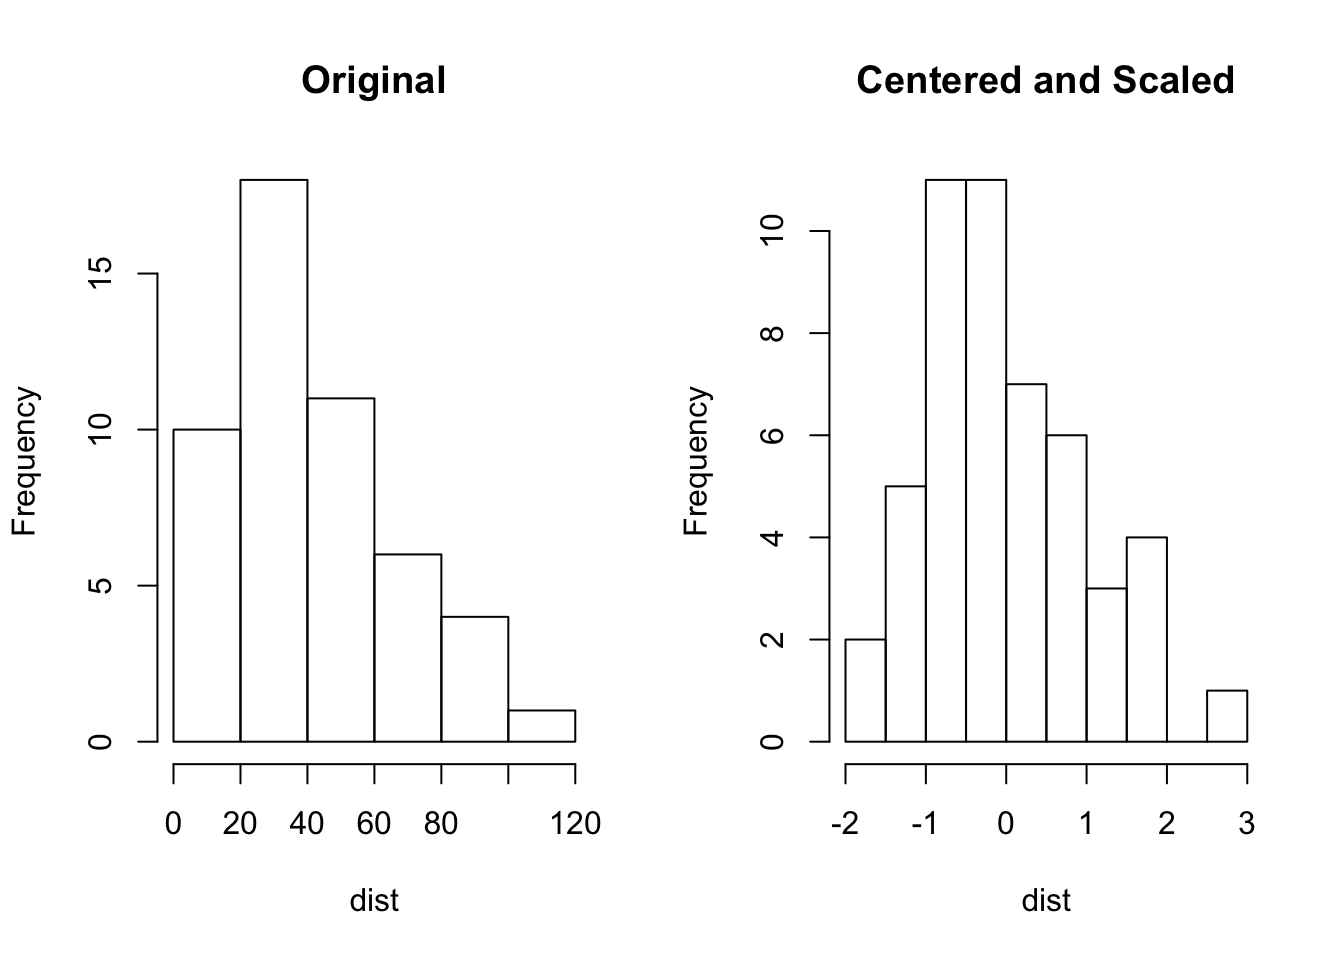
\includegraphics{IDS_files/figure-latex/unnamed-chunk-11-1.pdf}

Before the transformation, the \texttt{stroe\_trans} is skewed right.
\texttt{BoxCoxTrans\ ()} can also conduct Box-Cox transform. But note
that \texttt{BoxCoxTrans\ ()} can only be applied to a single variable,
and it is not possible to transform difference columns in a data frame
at the same time.

\begin{Shaded}
\begin{Highlighting}[]
\NormalTok{(trans <-}\StringTok{ }\KeywordTok{BoxCoxTrans}\NormalTok{(dat_bc}\OperatorTok{$}\NormalTok{store_trans))}
\end{Highlighting}
\end{Shaded}

\begin{verbatim}
## Box-Cox Transformation
## 
## 1000 data points used to estimate Lambda
## 
## Input data summary:
##    Min. 1st Qu.  Median    Mean 3rd Qu.    Max. 
##    1.00    3.00    4.00    5.35    7.00   20.00 
## 
## Largest/Smallest: 20 
## Sample Skewness: 1.11 
## 
## Estimated Lambda: 0.1 
## With fudge factor, Lambda = 0 will be used for transformations
\end{verbatim}

\begin{Shaded}
\begin{Highlighting}[]
\NormalTok{transformed <-}\StringTok{ }\KeywordTok{predict}\NormalTok{(trans, dat_bc}\OperatorTok{$}\NormalTok{store_trans)}
\KeywordTok{skewness}\NormalTok{(transformed)}
\end{Highlighting}
\end{Shaded}

\begin{verbatim}
## [1] -0.2155
\end{verbatim}

The estimate of \(\lambda\) is the same as before (0.1). The skewness of
the original observation is 1.1, and -0.2 after transformation. Although
it is not strictly 0, it is greatly improved.

\section{Resolve Outliers}\label{resolve-outliers}

Even under certain assumptions we can statistically define outliers, it
can be hard to define in some situations. Box plot, histogram and some
other basic visualizations can be used to initially check whether there
are outliers. For example, we can visualize numerical non-survey
variables in \texttt{sim.dat}:

\begin{Shaded}
\begin{Highlighting}[]
\CommentTok{# select numerical non-survey data}
\NormalTok{sdat<-}\KeywordTok{subset}\NormalTok{(sim.dat,}\DataTypeTok{select=}\KeywordTok{c}\NormalTok{(}\StringTok{"age"}\NormalTok{,}\StringTok{"income"}\NormalTok{,}\StringTok{"store_exp"}\NormalTok{,}\StringTok{"online_exp"}\NormalTok{,}\StringTok{"store_trans"}\NormalTok{,}\StringTok{"online_trans"}\NormalTok{ ))}
\CommentTok{# use scatterplotMatrix() function from car package}
\KeywordTok{par}\NormalTok{(}\DataTypeTok{oma=}\KeywordTok{c}\NormalTok{(}\DecValTok{2}\NormalTok{,}\DecValTok{2}\NormalTok{,}\DecValTok{1}\NormalTok{,}\DecValTok{2}\NormalTok{))}
\KeywordTok{scatterplotMatrix}\NormalTok{(sdat,}\DataTypeTok{diagonal=}\StringTok{"boxplot"}\NormalTok{,}\DataTypeTok{smoother=}\OtherTok{FALSE}\NormalTok{)}
\end{Highlighting}
\end{Shaded}

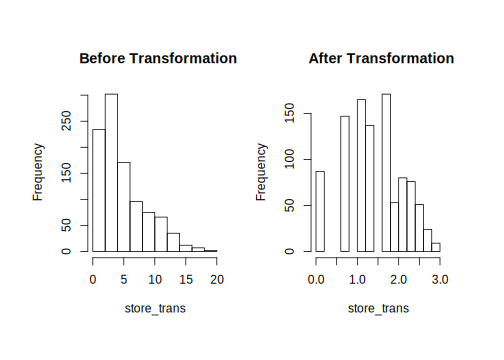
\includegraphics{IDS_files/figure-latex/unnamed-chunk-14-1.pdf}

It is also easy to observe the pair relationship from the plot.
\texttt{age} is negatively correlated with \texttt{online\_trans} but
positively correlated with \texttt{store\_trans}. It seems that older
people tend to purchase from the local store. The amount of expense is
positively correlated with income. Scatterplot matrix like this can
reveal lots of information before modeling.

In addition to visualization, there are some statistical methods to
define outliers, such as the commonly used Z-score. The Z-score for
variable \(\mathbf{Y}\) is defined as:

\[Z_{i}=\frac{Y_{i}-\bar{Y}}{s}\]

where \(\bar{Y}\) and \(s\) are mean and standard deviation for \(Y\).
Z-score is a measurement of the distance between each observation and
the mean. This method may be misleading, especially when the sample size
is small. Iglewicz and Hoaglin proposed to use the modified Z-score to
determine the outlier\citep{mad1}:

\[M_{i}=\frac{0.6745(Y_{i}-\bar{Y})}{MAD}\]

Where MAD is the median of a series of \(|Y_ {i} - \bar{Y}|\), called
the median of the absolute dispersion. Iglewicz and Hoaglin suggest that
the points with the Z-score greater than 3.5 corrected above are
possible outliers. Let's apply it to \texttt{income}:

\begin{Shaded}
\begin{Highlighting}[]
\CommentTok{# calculate median of the absolute dispersion for income}
\NormalTok{ymad <-}\StringTok{ }\KeywordTok{mad}\NormalTok{(}\KeywordTok{na.omit}\NormalTok{(sdat}\OperatorTok{$}\NormalTok{income))}
\CommentTok{# calculate z-score}
\NormalTok{zs <-}\StringTok{ }\NormalTok{(sdat}\OperatorTok{$}\NormalTok{income }\OperatorTok{-}\StringTok{ }\KeywordTok{mean}\NormalTok{(}\KeywordTok{na.omit}\NormalTok{(sdat}\OperatorTok{$}\NormalTok{income)))}\OperatorTok{/}\NormalTok{ymad}
\CommentTok{# count the number of outliers}
\KeywordTok{sum}\NormalTok{(}\KeywordTok{na.omit}\NormalTok{(zs }\OperatorTok{>}\StringTok{ }\FloatTok{3.5}\NormalTok{))}
\end{Highlighting}
\end{Shaded}

\begin{verbatim}
## [1] 59
\end{verbatim}

According to modified Z-score, variable income has 59 outliers. Refer to
\citep{mad1} for other ways of detecting outliers.

The impact of outliers depends on the model. Some models are sensitive
to outliers, such as linear regression, logistic regression. Some are
pretty robust to outliers, such as tree models, support vector machine.
Also, the outlier is not wrong data. It is real observation so cannot be
deleted at will. If a model is sensitive to outliers, we can use
\emph{spatial sign transformation} \citep{ssp} to minimize the problem.
It projects the original sample points to the surface of a sphere by:

\[x_{ij}^{*}=\frac{x_{ij}}{\sqrt{\sum_{j=1}^{p}x_{ij}^{2}}}\]

where \(x_{ij}\) represents the \(i^{th}\) observation and \(j^{th}\)
variable. As shown in the equation, every observation for sample \(i\)
is divided by its square mode. The denominator is the Euclidean distance
to the center of the p-dimensional predictor space. Three things to pay
attention here:

\begin{enumerate}
\def\labelenumi{\arabic{enumi}.}
\tightlist
\item
  It is important to center and scale the predictor data before using
  this transformation
\item
  Unlike centering or scaling, this manipulation of the predictors
  transforms them as a group
\item
  If there are some variables to remove (for example, highly correlated
  variables), do it before the transformation
\end{enumerate}

Function \texttt{spatialSign()} \texttt{caret} package can conduct the
transformation. Take \texttt{income} and \texttt{age} as an example:

\begin{Shaded}
\begin{Highlighting}[]
\CommentTok{# KNN imputation}
\NormalTok{sdat <-}\StringTok{ }\NormalTok{sim.dat[, }\KeywordTok{c}\NormalTok{(}\StringTok{"income"}\NormalTok{, }\StringTok{"age"}\NormalTok{)]}
\NormalTok{imp <-}\StringTok{ }\KeywordTok{preProcess}\NormalTok{(sdat, }\DataTypeTok{method =} \KeywordTok{c}\NormalTok{(}\StringTok{"knnImpute"}\NormalTok{), }\DataTypeTok{k =} \DecValTok{5}\NormalTok{)}
\NormalTok{sdat <-}\StringTok{ }\KeywordTok{predict}\NormalTok{(imp, sdat)}
\NormalTok{transformed <-}\StringTok{ }\KeywordTok{spatialSign}\NormalTok{(sdat)}
\NormalTok{transformed <-}\StringTok{ }\KeywordTok{as.data.frame}\NormalTok{(transformed)}
\KeywordTok{par}\NormalTok{(}\DataTypeTok{mfrow =} \KeywordTok{c}\NormalTok{(}\DecValTok{1}\NormalTok{, }\DecValTok{2}\NormalTok{), }\DataTypeTok{oma =} \KeywordTok{c}\NormalTok{(}\DecValTok{2}\NormalTok{, }\DecValTok{2}\NormalTok{, }\DecValTok{2}\NormalTok{, }\DecValTok{2}\NormalTok{))}
\KeywordTok{plot}\NormalTok{(income }\OperatorTok{~}\StringTok{ }\NormalTok{age, }\DataTypeTok{data =}\NormalTok{ sdat, }\DataTypeTok{col =} \StringTok{"blue"}\NormalTok{, }\DataTypeTok{main =} \StringTok{"Before"}\NormalTok{)}
\KeywordTok{plot}\NormalTok{(income }\OperatorTok{~}\StringTok{ }\NormalTok{age, }\DataTypeTok{data =}\NormalTok{ transformed, }\DataTypeTok{col =} \StringTok{"blue"}\NormalTok{, }\DataTypeTok{main =} \StringTok{"After"}\NormalTok{)}
\end{Highlighting}
\end{Shaded}

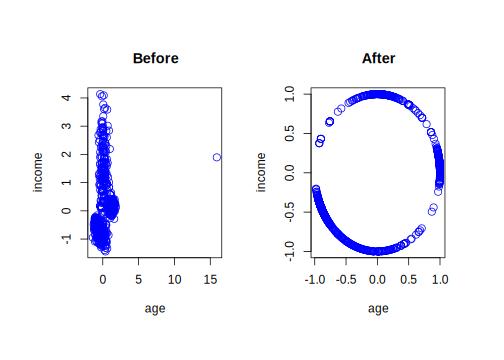
\includegraphics{IDS_files/figure-latex/unnamed-chunk-16-1.pdf}

Some readers may have found that the above code does not seem to
standardize the data before transformation. Recall the introduction of
KNN, \texttt{preProcess()} with \texttt{method="knnImpute"} by default
will standardize data.

\section{Collinearity}\label{collinearity}

It is probably the technical term known by the most un-technical people.
When two predictors are very strongly correlated, including both in a
model may lead to confusion or problem with a singular matrix. There is
an excellent function in \texttt{corrplot} package with the same name
\texttt{corrplot()} that can visualize correlation structure of a set of
predictors. The function has the option to reorder the variables in a
way that reveals clusters of highly correlated ones.

\begin{Shaded}
\begin{Highlighting}[]
\CommentTok{# select non-survey numerical variables}
\NormalTok{sdat <-}\StringTok{ }\KeywordTok{subset}\NormalTok{(sim.dat, }\DataTypeTok{select =} \KeywordTok{c}\NormalTok{(}\StringTok{"age"}\NormalTok{, }\StringTok{"income"}\NormalTok{, }\StringTok{"store_exp"}\NormalTok{, }\StringTok{"online_exp"}\NormalTok{, }
    \StringTok{"store_trans"}\NormalTok{, }\StringTok{"online_trans"}\NormalTok{))}
\CommentTok{# use bagging imputation here}
\NormalTok{imp <-}\StringTok{ }\KeywordTok{preProcess}\NormalTok{(sdat, }\DataTypeTok{method =} \StringTok{"bagImpute"}\NormalTok{)}
\NormalTok{sdat <-}\StringTok{ }\KeywordTok{predict}\NormalTok{(imp, sdat)}
\CommentTok{# get the correlation matrix}
\NormalTok{correlation <-}\StringTok{ }\KeywordTok{cor}\NormalTok{(sdat)}
\CommentTok{# plot}
\KeywordTok{par}\NormalTok{(}\DataTypeTok{oma =} \KeywordTok{c}\NormalTok{(}\DecValTok{2}\NormalTok{, }\DecValTok{2}\NormalTok{, }\DecValTok{2}\NormalTok{, }\DecValTok{2}\NormalTok{))}
\KeywordTok{corrplot.mixed}\NormalTok{(correlation, }\DataTypeTok{order =} \StringTok{"hclust"}\NormalTok{, }\DataTypeTok{tl.pos =} \StringTok{"lt"}\NormalTok{, }\DataTypeTok{upper =} \StringTok{"ellipse"}\NormalTok{)}
\end{Highlighting}
\end{Shaded}

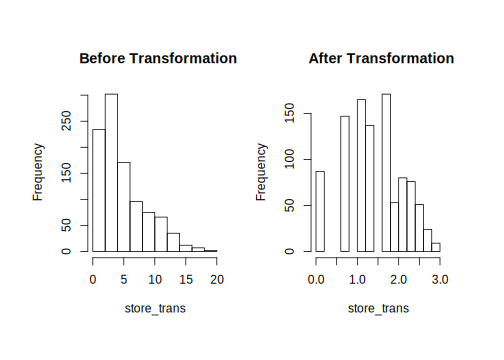
\includegraphics{IDS_files/figure-latex/unnamed-chunk-17-1.pdf}

The closer the correlation is to 0, the lighter the color is and the
closer the shape is to a circle. The elliptical means the correlation is
not equal to 0 (because we set the \texttt{upper\ =\ "ellipse"}), the
greater the correlation, the narrower the ellipse. Blue represents a
positive correlation; red represents a negative correlation. The
direction of the ellipse also changes with the correlation. The
correlation coefficient is shown in the lower triangle of the matrix.

The variables relationship from previous scatter matrix are clear here:
the negative correlation between age and online shopping, the positive
correlation between income and amount of purchasing. Some correlation is
very strong ( such as the correlation between \texttt{online\_trans}
and\texttt{age} is -0.7414) which means the two variables contain
duplicate information.

Section 3.5 of ``Applied Predictive Modeling'' \citep{APM} presents a
heuristic algorithm to remove a minimum number of predictors to ensure
all pairwise correlations are below a certain threshold:

\begin{quote}
\begin{enumerate}
\def\labelenumi{(\arabic{enumi})}
\tightlist
\item
  Calculate the correlation matrix of the predictors.
\item
  Determine the two predictors associated with the largest absolute
  pairwise correlation (call them predictors A and B).
\item
  Determine the average correlation between A and the other variables.
  Do the same for predictor B.
\item
  If A has a larger average correlation, remove it; otherwise, remove
  predictor B.
\item
  Repeat Step 2-4 until no absolute correlations are above the
  threshold.
\end{enumerate}
\end{quote}

The \texttt{findCorrelation()} function in package \texttt{caret} will
apply the above algorithm.

\begin{Shaded}
\begin{Highlighting}[]
\NormalTok{(highCorr <-}\StringTok{ }\KeywordTok{findCorrelation}\NormalTok{(}\KeywordTok{cor}\NormalTok{(sdat), }\DataTypeTok{cutoff =} \FloatTok{0.7}\NormalTok{))}
\end{Highlighting}
\end{Shaded}

\begin{verbatim}
## [1] 2 6
\end{verbatim}

It returns the index of columns need to be deleted. It tells us that we
need to remove the first column to make sure the correlations are all
below 0.7.

\begin{Shaded}
\begin{Highlighting}[]
\CommentTok{# delete highly correlated columns}
\NormalTok{sdat <-}\StringTok{ }\NormalTok{sdat[}\OperatorTok{-}\NormalTok{highCorr]}
\CommentTok{# check the new correlation matrix}
\NormalTok{(}\KeywordTok{cor}\NormalTok{(sdat))}
\end{Highlighting}
\end{Shaded}

The absolute value of the elements in the correlation matrix after
removal are all below 0.7. How strong does a correlation have to get,
before you should start worrying about multicollinearity? There is no
easy answer to that question. You can treat the threshold as a tuning
parameter and pick one that gives you best prediction accuracy.

\section{Sparse Variables}\label{sparse-variables}

Other than the highly related predictors, predictors with degenerate
distributions can cause the problem too. Removing those variables can
significantly improve some models' performance and stability (such as
linear regression and logistic regression but the tree based model is
impervious to this type of predictors). One extreme example is a
variable with a single value which is called zero-variance variable.
Variables with very low frequency of unique values are near-zero
variance predictors. In general, detecting those variables follows two
rules:

\begin{itemize}
\tightlist
\item
  The fraction of unique values over the sample size
\item
  The ratio of the frequency of the most prevalent value to the
  frequency of the second most prevalent value.
\end{itemize}

\texttt{nearZeroVar()} function in the \texttt{caret} package can filter
near-zero variance predictors according to the above rules. In order to
show the useage of the function, let's arbitaryly add some problematic
variables to the origional data \texttt{sim.dat}:

\begin{Shaded}
\begin{Highlighting}[]
\CommentTok{# make a copy}
\NormalTok{zero_demo <-}\StringTok{ }\NormalTok{sim.dat}
\CommentTok{# add two sparse variable zero1 only has one unique value zero2 is a}
\CommentTok{# vector with the first element 1 and the rest are 0s}
\NormalTok{zero_demo}\OperatorTok{$}\NormalTok{zero1 <-}\StringTok{ }\KeywordTok{rep}\NormalTok{(}\DecValTok{1}\NormalTok{, }\KeywordTok{nrow}\NormalTok{(zero_demo))}
\NormalTok{zero_demo}\OperatorTok{$}\NormalTok{zero2 <-}\StringTok{ }\KeywordTok{c}\NormalTok{(}\DecValTok{1}\NormalTok{, }\KeywordTok{rep}\NormalTok{(}\DecValTok{0}\NormalTok{, }\KeywordTok{nrow}\NormalTok{(zero_demo) }\OperatorTok{-}\StringTok{ }\DecValTok{1}\NormalTok{))}
\end{Highlighting}
\end{Shaded}

The function will return a vector of integers indicating which columns
to remove:

\begin{Shaded}
\begin{Highlighting}[]
\KeywordTok{nearZeroVar}\NormalTok{(zero_demo,}\DataTypeTok{freqCut =} \DecValTok{95}\OperatorTok{/}\DecValTok{5}\NormalTok{, }\DataTypeTok{uniqueCut =} \DecValTok{10}\NormalTok{)}
\end{Highlighting}
\end{Shaded}

\begin{verbatim}
## [1] 20 21
\end{verbatim}

As expected, it returns the two columns we generated. You can go ahead
to remove them. Note the two arguments in the function
\texttt{freqCut\ =} and \texttt{uniqueCut\ =} are corresponding to the
previous two rules.

\begin{itemize}
\tightlist
\item
  \texttt{freqCut}: the cutoff for the ratio of the most common value to
  the second most common value
\item
  \texttt{uniqueCut}: the cutoff for the percentage of distinct values
  out of the number of total samples
\end{itemize}

\section{Re-encode Dummy Variables}\label{re-encode-dummy-variables}

A dummy variable is a binary variable (0/1) to represent subgroups of
the sample. Sometimes we need to recode categories to smaller bits of
information named ``dummy variables.'' For example, some questionnaires
have five options for each question, A, B, C, D, and E. After you get
the data, you will usually convert the corresponding categorical
variables for each question into five nominal variables, and then use
one of the options as the baseline.

Let's encode \texttt{gender} and \texttt{house} from \texttt{sim.dat} to
dummy variables. There are two ways to implement this. The first is to
use \texttt{class.ind()} from \texttt{nnet} package. However, it only
works on one variable at a time.

\begin{Shaded}
\begin{Highlighting}[]
\NormalTok{dumVar <-}\StringTok{ }\NormalTok{nnet}\OperatorTok{::}\KeywordTok{class.ind}\NormalTok{(sim.dat}\OperatorTok{$}\NormalTok{gender)}
\KeywordTok{head}\NormalTok{(dumVar)}
\end{Highlighting}
\end{Shaded}

\begin{verbatim}
##      Female Male
## [1,]      1    0
## [2,]      1    0
## [3,]      0    1
## [4,]      0    1
## [5,]      0    1
## [6,]      0    1
\end{verbatim}

Since it is redundant to keep both, we need to remove one of them when
modeling. Another more powerful function is \texttt{dummyVars()} from
\texttt{caret}:

\begin{Shaded}
\begin{Highlighting}[]
\CommentTok{# use "origional variable name + level" as new name}
\NormalTok{dumMod <-}\StringTok{ }\KeywordTok{dummyVars}\NormalTok{(}\OperatorTok{~}\NormalTok{gender }\OperatorTok{+}\StringTok{ }\NormalTok{house }\OperatorTok{+}\StringTok{ }\NormalTok{income, }
                    \DataTypeTok{data =}\NormalTok{ sim.dat, }
                    \DataTypeTok{levelsOnly =}\NormalTok{ F)}
\KeywordTok{head}\NormalTok{(}\KeywordTok{predict}\NormalTok{(dumMod, sim.dat))}
\end{Highlighting}
\end{Shaded}

\begin{verbatim}
##   gender.Female gender.Male house.No house.Yes income
## 1             1           0        0         1 120963
## 2             1           0        0         1 122008
## 3             0           1        0         1 114202
## 4             0           1        0         1 113616
## 5             0           1        0         1 124253
## 6             0           1        0         1 107661
\end{verbatim}

\texttt{dummyVars()} can also use formula format. The variable on the
right-hand side can be both categorical and numeric. For a numerical
variable, the function will keep the variable unchanged. The advantage
is that you can apply the function to a data frame without removing
numerical variables. Other than that, the function can create
interaction term:

\begin{Shaded}
\begin{Highlighting}[]
\NormalTok{dumMod <-}\StringTok{ }\KeywordTok{dummyVars}\NormalTok{(}\OperatorTok{~}\NormalTok{gender }\OperatorTok{+}\StringTok{ }\NormalTok{house }\OperatorTok{+}\StringTok{ }\NormalTok{income }\OperatorTok{+}\StringTok{ }\NormalTok{income}\OperatorTok{:}\NormalTok{gender, }
                    \DataTypeTok{data =}\NormalTok{ sim.dat, }
                    \DataTypeTok{levelsOnly =}\NormalTok{ F)}
\KeywordTok{head}\NormalTok{(}\KeywordTok{predict}\NormalTok{(dumMod, sim.dat))}
\end{Highlighting}
\end{Shaded}

\begin{verbatim}
##   gender.Female gender.Male house.No house.Yes income
## 1             1           0        0         1 120963
## 2             1           0        0         1 122008
## 3             0           1        0         1 114202
## 4             0           1        0         1 113616
## 5             0           1        0         1 124253
## 6             0           1        0         1 107661
##   gender.Female:income gender.Male:income
## 1               120963                  0
## 2               122008                  0
## 3                    0             114202
## 4                    0             113616
## 5                    0             124253
## 6                    0             107661
\end{verbatim}

If you think the impact income levels on purchasing behavior is
different for male and female, then you may add the interaction term
between \texttt{income} and \texttt{gender}. You can do this by adding
\texttt{income:\ gender} in the formula.

\chapter{Data Wrangling}\label{data-wrangling}

This chapter focuses on some of the most frequently used data
manipulations and shows how to implement them in R and Python. It is
critical to explore the data with descriptive statistics (mean, standard
deviation, etc.) and data visualization before analysis. Transform data
so that the data structure is in line with the requirements of the
model. You also need to summarize the results after analysis.

Load the R packages first:

\begin{Shaded}
\begin{Highlighting}[]
\CommentTok{# install packages from CRAN}
\NormalTok{p_needed <-}\StringTok{ }\KeywordTok{c}\NormalTok{(}\StringTok{'readr'}\NormalTok{,}\StringTok{'dplyr'}\NormalTok{,}\StringTok{'data.table'}\NormalTok{,}\StringTok{'reshape2'}\NormalTok{,}\StringTok{'tidyr'}\NormalTok{)}
\NormalTok{packages <-}\StringTok{ }\KeywordTok{rownames}\NormalTok{(}\KeywordTok{installed.packages}\NormalTok{())}
\NormalTok{p_to_install <-}\StringTok{ }\NormalTok{p_needed[}\OperatorTok{!}\NormalTok{(p_needed }\OperatorTok\StringTok{ }\NormalTok{packages)]}
\ControlFlowTok{if}\NormalTok{ (}\KeywordTok{length}\NormalTok{(p_to_install) }\OperatorTok{>}\StringTok{ }\DecValTok{0}\NormalTok{) \{}
    \KeywordTok{install.packages}\NormalTok{(p_to_install)}
\NormalTok{\}}

\KeywordTok{lapply}\NormalTok{(p_needed, require, }\DataTypeTok{character.only =} \OtherTok{TRUE}\NormalTok{)}
\end{Highlighting}
\end{Shaded}

\section{Read and write data}\label{read-and-write-data}

\subsection{\texorpdfstring{\texttt{readr}}{readr}}\label{readr}

You must be familiar with \texttt{read.csv()}, \texttt{read.table()} and
\texttt{write.csv()} in base R. Here we will introduce a more efficient
package from RStudio in 2015 for reading and writing data:
\texttt{readr} package. The corresponding functions are
\texttt{read\_csv()}, \texttt{read\_table()} and \texttt{write\_csv()}.
The commands look quite similar, but \texttt{readr} is different in the
following respects:

\begin{enumerate}
\def\labelenumi{\arabic{enumi}.}
\item
  It is 10x faster. The trick is that \texttt{readr} uses C++ to process
  the data quickly.
\item
  It doesn't change the column names. The names can start with a number
  and ``\texttt{.}'' will not be substituted to ``\texttt{\_}''. For
  example:
\end{enumerate}

\begin{Shaded}
\begin{Highlighting}[]
\KeywordTok{read_csv}\NormalTok{(}\StringTok{"2015,2016,2017}
\StringTok{1,2,3}
\StringTok{4,5,6"}\NormalTok{)}
\end{Highlighting}
\end{Shaded}

\begin{verbatim}
## # A tibble: 2 x 3
##   `2015` `2016` `2017`
##    <int>  <int>  <int>
## 1      1      2      3
## 2      4      5      6
\end{verbatim}

\begin{enumerate}
\def\labelenumi{\arabic{enumi}.}
\item
  \texttt{readr} functions do not convert strings to factors by default,
  are able to parse dates and times and can automatically determine the
  data types in each column.
\item
  The killing character, in my opinion, is that \texttt{readr} provides
  \textbf{progress bar}. What makes you feel worse than waiting is not
  knowing how long you have to wait.
\end{enumerate}

\begin{figure}
\centering
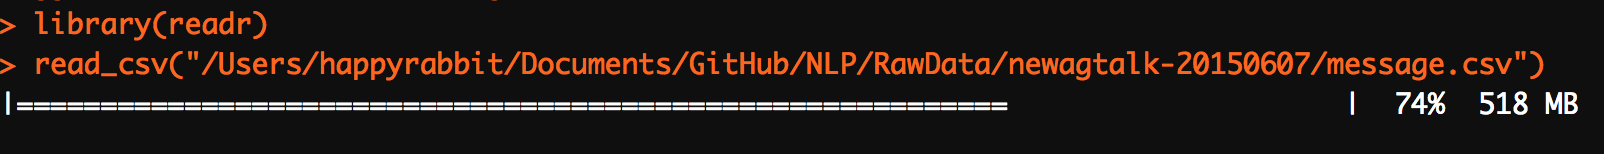
\includegraphics{images/prograssbar.png}
\caption{}
\end{figure}

The major functions of readr is to turn flat files into data frames:

\begin{itemize}
\tightlist
\item
  \texttt{read\_csv()}: reads comma delimited files
\item
  \texttt{read\_csv2()}: reads semicolon separated files (common in
  countries where \texttt{,} is used as the decimal place)
\item
  \texttt{read\_tsv()}: reads tab delimited files
\item
  \texttt{read\_delim()}: reads in files with any delimiter
\item
  \texttt{read\_fwf()}: reads fixed width files. You can specify fields
  either by their widths with \texttt{fwf\_widths()} or their position
  with \texttt{fwf\_positions()}\\
\item
  \texttt{read\_table()}: reads a common variation of fixed width files
  where columns are separated by white space
\item
  \texttt{read\_log()}: reads Apache style log files
\end{itemize}

The good thing is that those functions have similar syntax. Once you
learn one, the others become easy. Here we will focus on
\texttt{read\_csv()}.

The most important information for \texttt{read\_csv()} is the path to
your data:

\begin{Shaded}
\begin{Highlighting}[]
\NormalTok{sim.dat <-}\StringTok{ }\KeywordTok{read_csv}\NormalTok{(}\StringTok{"http://bit.ly/2P5gTw4"}\NormalTok{)}
\KeywordTok{head}\NormalTok{(sim.dat)}
\end{Highlighting}
\end{Shaded}

\begin{verbatim}
# A tibble: 6 x 19
    age gender income house store_exp online_exp store_trans online_trans    Q1
  <int> <chr>   <dbl> <chr>     <dbl>      <dbl>       <int>        <int> <int>
1    57 Female 1.21e5 Yes        529.       304.           2            2     4
2    63 Female 1.22e5 Yes        478.       110.           4            2     4
3    59 Male   1.14e5 Yes        491.       279.           7            2     5
4    60 Male   1.14e5 Yes        348.       142.          10            2     5
5    51 Male   1.24e5 Yes        380.       112.           4            4     4
6    59 Male   1.08e5 Yes        338.       196.           4            5     4
# ... with 10 more variables: Q2 <int>, Q3 <int>, Q4 <int>, Q5 <int>, Q6 <int>,
#   Q7 <int>, Q8 <int>, Q9 <int>, Q10 <int>, segment <chr>
\end{verbatim}

The function reads the file to R as a \texttt{tibble}. You can consider
\texttt{tibble} as next iteration of the data frame. They are different
with data frame for the following aspects:

\begin{itemize}
\tightlist
\item
  It never changes an input's type (i.e., no more
  \texttt{stringsAsFactors\ =\ FALSE}!)
\item
  It never adjusts the names of variables
\item
  It has a refined print method that shows only the first 10 rows and
  all the columns that fit on the screen. You can also control the
  default print behavior by setting options.
\end{itemize}

Refer to \url{http://r4ds.had.co.nz/tibbles.html} for more information
about `tibble'.

When you run \texttt{read\_csv()} it prints out a column specification
that gives the name and type of each column. To better understanding how
\texttt{readr} works, it is helpful to type in some baby data set and
check the results:

\begin{Shaded}
\begin{Highlighting}[]
\NormalTok{dat <-}\StringTok{ }\KeywordTok{read_csv}\NormalTok{(}\StringTok{"2015,2016,2017}
\StringTok{100,200,300}
\StringTok{canola,soybean,corn"}\NormalTok{)}
\KeywordTok{print}\NormalTok{(dat)}
\end{Highlighting}
\end{Shaded}

\begin{verbatim}
## # A tibble: 2 x 3
##   `2015` `2016`  `2017`
##   <chr>  <chr>   <chr> 
## 1 100    200     300   
## 2 canola soybean corn
\end{verbatim}

You can also add comments on the top and tell R to skip those lines:

\begin{Shaded}
\begin{Highlighting}[]
\NormalTok{dat <-}\StringTok{ }\KeywordTok{read_csv}\NormalTok{(}\StringTok{"# I will never let you know that}
\StringTok{          # my favorite food is carrot}
\StringTok{          Date,Food,Mood}
\StringTok{          Monday,carrot,happy}
\StringTok{          Tuesday,carrot,happy}
\StringTok{          Wednesday,carrot,happy}
\StringTok{          Thursday,carrot,happy}
\StringTok{          Friday,carrot,happy}
\StringTok{          Saturday,carrot,extremely happy}
\StringTok{          Sunday,carrot,extremely happy"}\NormalTok{, }
          \DataTypeTok{skip =} \DecValTok{2}\NormalTok{)}
\KeywordTok{print}\NormalTok{(dat)}
\end{Highlighting}
\end{Shaded}

\begin{verbatim}
## # A tibble: 7 x 3
##   Date      Food   Mood           
##   <chr>     <chr>  <chr>          
## 1 Monday    carrot happy          
## 2 Tuesday   carrot happy          
## 3 Wednesday carrot happy          
## 4 Thursday  carrot happy          
## 5 Friday    carrot happy          
## 6 Saturday  carrot extremely happy
## 7 Sunday    carrot extremely happy
\end{verbatim}

If you don't have column names, set \texttt{col\_names\ =\ FALSE} then R
will assign names ``\texttt{X1}'',``\texttt{X2}''\ldots{} to the
columns:

\begin{Shaded}
\begin{Highlighting}[]
\NormalTok{dat <-}\StringTok{ }\KeywordTok{read_csv}\NormalTok{(}\StringTok{"Saturday,carrot,extremely happy}
\StringTok{          Sunday,carrot,extremely happy"}\NormalTok{, }\DataTypeTok{col_names =} \OtherTok{FALSE}\NormalTok{)}
\KeywordTok{print}\NormalTok{(dat)}
\end{Highlighting}
\end{Shaded}

\begin{verbatim}
## # A tibble: 2 x 3
##   X1       X2     X3             
##   <chr>    <chr>  <chr>          
## 1 Saturday carrot extremely happy
## 2 Sunday   carrot extremely happy
\end{verbatim}

You can also pass \texttt{col\_names} a character vector which will be
used as the column names. Try to replace \texttt{col\_names=FALSE} with
\texttt{col\_names=c("Date","Food","Mood")} and see what happen.

As mentioned before, you can use \texttt{read\_csv2()} to read semicolon
separated files:

\begin{Shaded}
\begin{Highlighting}[]
\NormalTok{dat <-}\StringTok{ }\KeywordTok{read_csv2}\NormalTok{(}\StringTok{"Saturday; carrot; extremely happy }\CharTok{\textbackslash{}n}\StringTok{ Sunday; carrot; extremely happy"}\NormalTok{, }\DataTypeTok{col_names =} \OtherTok{FALSE}\NormalTok{)}
\end{Highlighting}
\end{Shaded}

\begin{verbatim}
## Using ',' as decimal and '.' as grouping mark. Use read_delim() for more control.
\end{verbatim}

\begin{Shaded}
\begin{Highlighting}[]
\KeywordTok{print}\NormalTok{(dat)}
\end{Highlighting}
\end{Shaded}

\begin{verbatim}
## # A tibble: 2 x 3
##   X1       X2     X3             
##   <chr>    <chr>  <chr>          
## 1 Saturday carrot extremely happy
## 2 Sunday   carrot extremely happy
\end{verbatim}

Here ``\texttt{\textbackslash{}n}'' is a convenient shortcut for adding
a new line.

You can use \texttt{read\_tsv()} to read tab delimited files:

\begin{Shaded}
\begin{Highlighting}[]
\NormalTok{dat <-}\StringTok{ }\KeywordTok{read_tsv}\NormalTok{(}\StringTok{"every}\CharTok{\textbackslash{}t}\StringTok{man}\CharTok{\textbackslash{}t}\StringTok{is}\CharTok{\textbackslash{}t}\StringTok{a}\CharTok{\textbackslash{}t}\StringTok{poet}\CharTok{\textbackslash{}t}\StringTok{when}\CharTok{\textbackslash{}t}\StringTok{he}\CharTok{\textbackslash{}t}\StringTok{is}\CharTok{\textbackslash{}t}\StringTok{in}\CharTok{\textbackslash{}t}\StringTok{love}\CharTok{\textbackslash{}n}\StringTok{"}\NormalTok{, }
    \DataTypeTok{col_names =} \OtherTok{FALSE}\NormalTok{)}
\KeywordTok{print}\NormalTok{(dat)}
\end{Highlighting}
\end{Shaded}

\begin{verbatim}
## # A tibble: 1 x 10
##   X1    X2    X3    X4    X5    X6    X7    X8   
##   <chr> <chr> <chr> <chr> <chr> <chr> <chr> <chr>
## 1 every man   is    a     poet  when  he    is   
## # ... with 2 more variables: X9 <chr>, X10 <chr>
\end{verbatim}

Or more generally, you can use \texttt{read\_delim()} and assign
separating character:

\begin{Shaded}
\begin{Highlighting}[]
\NormalTok{dat <-}\StringTok{ }\KeywordTok{read_delim}\NormalTok{(}\StringTok{"THE|UNBEARABLE|RANDOMNESS|OF|LIFE}\CharTok{\textbackslash{}n}\StringTok{"}\NormalTok{, }
    \DataTypeTok{delim =} \StringTok{"|"}\NormalTok{, }\DataTypeTok{col_names =} \OtherTok{FALSE}\NormalTok{)}
\KeywordTok{print}\NormalTok{(dat)}
\end{Highlighting}
\end{Shaded}

\begin{verbatim}
## # A tibble: 1 x 5
##   X1    X2         X3         X4    X5   
##   <chr> <chr>      <chr>      <chr> <chr>
## 1 THE   UNBEARABLE RANDOMNESS OF    LIFE
\end{verbatim}

Another situation you will often run into is the missing value. In
marketing survey, people like to use ``99'' to represent missing. You
can tell R to set all observation with value ``99'' as missing when you
read the data:

\begin{Shaded}
\begin{Highlighting}[]
\NormalTok{dat <-}\StringTok{ }\KeywordTok{read_csv}\NormalTok{(}\StringTok{"Q1,Q2,Q3}
\StringTok{               5, 4,99"}\NormalTok{, }
               \DataTypeTok{na =} \StringTok{"99"}\NormalTok{)}
\KeywordTok{print}\NormalTok{(dat)}
\end{Highlighting}
\end{Shaded}

\begin{verbatim}
## # A tibble: 1 x 3
##      Q1    Q2 Q3   
##   <int> <int> <chr>
## 1     5     4 <NA>
\end{verbatim}

For writing data back to disk, you can use \texttt{write\_csv()} and
\texttt{write\_tsv()}. The following two characters of the two functions
increase the chances of the output file being read back in correctly:

\begin{itemize}
\tightlist
\item
  Encode strings in UTF-8
\item
  Save dates and date-times in ISO8601 format so they are easily parsed
  elsewhere
\end{itemize}

For example:

\begin{Shaded}
\begin{Highlighting}[]
\KeywordTok{write_csv}\NormalTok{(sim.dat, }\StringTok{"sim_dat.csv"}\NormalTok{)}
\end{Highlighting}
\end{Shaded}

For other data types, you can use the following packages:

\begin{itemize}
\tightlist
\item
  \texttt{Haven}: SPSS, Stata and SAS data
\item
  \texttt{Readxl} and \texttt{xlsx}: excel data(.xls and .xlsx)
\item
  \texttt{DBI}: given data base, such as RMySQL, RSQLite and
  RPostgreSQL, read data directly from the database using SQL
\end{itemize}

Some other useful materials:

\begin{itemize}
\tightlist
\item
  For getting data from the internet, you can refer to the book ``XML
  and Web Technologies for Data Sciences with R''.\\
\item
  \href{https://cran.r-project.org/doc/manuals/r-release/R-data.html\#Acknowledgements}{R
  data import/export manual}
\item
  \texttt{rio} package:\url{https://github.com/leeper/rio}
\end{itemize}

\subsection{\texorpdfstring{\texttt{data.table}--- enhanced
\texttt{data.frame}}{data.table--- enhanced data.frame}}\label{data.table-enhanced-data.frame}

What is \texttt{data.table}? It is an R package that provides an
enhanced version of \texttt{data.frame}. The most used object in R is
\texttt{data\ frame}. Before we move on, let's briefly review some basic
characters and manipulations of data.frame:

\begin{itemize}
\tightlist
\item
  It is a set of rows and columns.
\item
  Each row is of the same length and data type
\item
  Every column is of the same length but can be of differing data types
\item
  It has characteristics of both a matrix and a list
\item
  It uses \texttt{{[}{]}} to subset data
\end{itemize}

We will use the clothes customer data to illustrate. There are two
dimensions in \texttt{{[}{]}}. The first one indicates the row and
second one indicates column. It uses a comma to separate them.

\begin{Shaded}
\begin{Highlighting}[]
\CommentTok{# read data}
\NormalTok{sim.dat <-}\StringTok{ }\NormalTok{readr}\OperatorTok{::}\KeywordTok{read_csv}\NormalTok{(}\StringTok{"http://bit.ly/2P5gTw4"}\NormalTok{)}
\end{Highlighting}
\end{Shaded}

\begin{verbatim}
## Parsed with column specification:
## cols(
##   age = col_integer(),
##   gender = col_character(),
##   income = col_double(),
##   house = col_character(),
##   store_exp = col_double(),
##   online_exp = col_double(),
##   store_trans = col_integer(),
##   online_trans = col_integer(),
##   Q1 = col_integer(),
##   Q2 = col_integer(),
##   Q3 = col_integer(),
##   Q4 = col_integer(),
##   Q5 = col_integer(),
##   Q6 = col_integer(),
##   Q7 = col_integer(),
##   Q8 = col_integer(),
##   Q9 = col_integer(),
##   Q10 = col_integer(),
##   segment = col_character()
## )
\end{verbatim}

\begin{Shaded}
\begin{Highlighting}[]
\CommentTok{# subset the first two rows}
\NormalTok{sim.dat[}\DecValTok{1}\OperatorTok{:}\DecValTok{2}\NormalTok{, ]}
\CommentTok{# subset the first two rows and column 3 and 5}
\NormalTok{sim.dat[}\DecValTok{1}\OperatorTok{:}\DecValTok{2}\NormalTok{, }\KeywordTok{c}\NormalTok{(}\DecValTok{3}\NormalTok{, }\DecValTok{5}\NormalTok{)]}
\CommentTok{# get all rows with age>70}
\NormalTok{sim.dat[sim.dat}\OperatorTok{$}\NormalTok{age }\OperatorTok{>}\StringTok{ }\DecValTok{70}\NormalTok{, ]}
\CommentTok{# get rows with age> 60 and gender is Male select column 3 and 4}
\NormalTok{sim.dat[sim.dat}\OperatorTok{$}\NormalTok{age }\OperatorTok{>}\StringTok{ }\DecValTok{68} \OperatorTok{&}\StringTok{ }\NormalTok{sim.dat}\OperatorTok{$}\NormalTok{gender }\OperatorTok{==}\StringTok{ "Male"}\NormalTok{, }\DecValTok{3}\OperatorTok{:}\DecValTok{4}\NormalTok{]}
\end{Highlighting}
\end{Shaded}

Remember that there are usually different ways to conduct the same
manipulation. For example, the following code presents three ways to
calculate an average number of online transactions for male and female:

\begin{Shaded}
\begin{Highlighting}[]
\KeywordTok{tapply}\NormalTok{(sim.dat}\OperatorTok{$}\NormalTok{online_trans, sim.dat}\OperatorTok{$}\NormalTok{gender, mean)}

\KeywordTok{aggregate}\NormalTok{(online_trans }\OperatorTok{~}\StringTok{ }\NormalTok{gender, }\DataTypeTok{data =}\NormalTok{ sim.dat, mean)}

\NormalTok{sim.dat }\OperatorTok\StringTok{ }
\StringTok{  }\KeywordTok{group_by}\NormalTok{(gender) }\OperatorTok\StringTok{ }
\StringTok{  }\KeywordTok{summarise}\NormalTok{(}\DataTypeTok{Avg_online_trans =} \KeywordTok{mean}\NormalTok{(online_trans))}
\end{Highlighting}
\end{Shaded}

There is no gold standard to choose a specific function to manipulate
data. The goal is to solve the real problem, not the tool itself. So
just use whatever tool that is convenient for you.

The way to use \texttt{{[}{]}} is straightforward. But the manipulations
are limited. If you need more complicated data reshaping or aggregation,
there are other packages to use such as \texttt{dplyr},
\texttt{reshape2}, \texttt{tidyr} etc. But the usage of those packages
are not as straightforward as \texttt{{[}{]}}. You often need to change
functions. Keeping related operations together, such as subset, group,
update, join etc, will allow for:

\begin{itemize}
\tightlist
\item
  concise, consistent and readable syntax irrespective of the set of
  operations you would like to perform to achieve your end goal
\item
  performing data manipulation fluidly without the cognitive burden of
  having to change among different functions
\item
  by knowing precisely the data required for each operation, you can
  automatically optimize operations effectively
\end{itemize}

\texttt{data.table} is the package for that. If you are not familiar
with other data manipulating packages and are interested in reducing
programming time tremendously, then this package is for you.

Other than extending the function of \texttt{{[}{]}},
\texttt{data.table} has the following advantages:

\begin{itemize}
\tightlist
\item
  Offers fast import, subset, grouping, update, and joins for large data
  files
\item
  It is easy to turn data frame to data table
\item
  Can behave just like a data frame
\end{itemize}

You need to install and load the package:

Use \texttt{data.table()} to convert the existing data frame
\texttt{sim.dat} to data table:

\begin{Shaded}
\begin{Highlighting}[]
\NormalTok{dt <-}\StringTok{ }\KeywordTok{data.table}\NormalTok{(sim.dat)}
\KeywordTok{class}\NormalTok{(dt)}
\end{Highlighting}
\end{Shaded}

\begin{verbatim}
## [1] "data.table" "data.frame"
\end{verbatim}

Calculate mean for counts of online transactions:

\begin{Shaded}
\begin{Highlighting}[]
\NormalTok{dt[, }\KeywordTok{mean}\NormalTok{(online_trans)]}
\end{Highlighting}
\end{Shaded}

\begin{verbatim}
## [1] 13.55
\end{verbatim}

You can't do the same thing using data frame:

\begin{Shaded}
\begin{Highlighting}[]
\NormalTok{sim.dat[,}\KeywordTok{mean}\NormalTok{(online_trans)]}
\end{Highlighting}
\end{Shaded}

\begin{Shaded}
\begin{Highlighting}[]
\NormalTok{Error in mean(online_trans) : object 'online_trans' not found}
\end{Highlighting}
\end{Shaded}

If you want to calculate mean by group as before, set ``\texttt{by\ =}''
argument:

\begin{Shaded}
\begin{Highlighting}[]
\NormalTok{dt[ , }\KeywordTok{mean}\NormalTok{(online_trans), by =}\StringTok{ }\NormalTok{gender]}
\end{Highlighting}
\end{Shaded}

\begin{verbatim}
##    gender    V1
## 1: Female 15.38
## 2:   Male 11.26
\end{verbatim}

You can group by more than one variables. For example, group by
``\texttt{gender}'' and ``\texttt{house}'':

\begin{Shaded}
\begin{Highlighting}[]
\NormalTok{dt[ , }\KeywordTok{mean}\NormalTok{(online_trans), by =}\StringTok{ }\NormalTok{.(gender, house)]}
\end{Highlighting}
\end{Shaded}

\begin{verbatim}
##    gender house     V1
## 1: Female   Yes 11.312
## 2:   Male   Yes  8.772
## 3: Female    No 19.146
## 4:   Male    No 16.486
\end{verbatim}

Assign column names for aggregated variables:

\begin{Shaded}
\begin{Highlighting}[]
\NormalTok{dt[ , .(}\DataTypeTok{avg =} \KeywordTok{mean}\NormalTok{(online_trans)), by =}\StringTok{ }\NormalTok{.(gender, house)]}
\end{Highlighting}
\end{Shaded}

\begin{verbatim}
##    gender house    avg
## 1: Female   Yes 11.312
## 2:   Male   Yes  8.772
## 3: Female    No 19.146
## 4:   Male    No 16.486
\end{verbatim}

\texttt{data.table} can accomplish all operations that
\texttt{aggregate()} and \texttt{tapply()}can do for data frame.

\begin{itemize}
\tightlist
\item
  General setting of \texttt{data.table}
\end{itemize}

Different from data frame, there are three arguments for data table:


\includegraphics{images/datable1.png}

It is analogous to SQL. You don't have to know SQL to learn data table.
But experience with SQL will help you understand data table. In SQL, you
select column \texttt{j} (use command \texttt{SELECT}) for row
\texttt{i} (using command \texttt{WHERE}). \texttt{GROUP\ BY} in SQL
will assign the variable to group the observations.

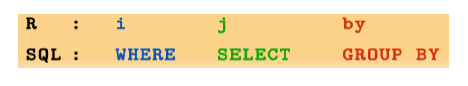
\includegraphics{images/rSQL.png}

Let's review our previous code:

\begin{Shaded}
\begin{Highlighting}[]
\NormalTok{dt[ , }\KeywordTok{mean}\NormalTok{(online_trans), by =}\StringTok{ }\NormalTok{gender]}
\end{Highlighting}
\end{Shaded}

The code above is equal to the following SQL:

\begin{Shaded}
\begin{Highlighting}[]
\KeywordTok{SELECT}\NormalTok{  gender, }\FunctionTok{avg}\NormalTok{(online_trans) }\KeywordTok{FROM}\NormalTok{ sim.dat }\KeywordTok{GROUP} \KeywordTok{BY}\NormalTok{ gender}
\end{Highlighting}
\end{Shaded}

R code:

\begin{Shaded}
\begin{Highlighting}[]
\NormalTok{dt[ , .(}\DataTypeTok{avg =} \KeywordTok{mean}\NormalTok{(online_trans)), by =}\StringTok{ }\NormalTok{.(gender, house)]}
\end{Highlighting}
\end{Shaded}

is equal to SQL:

\begin{Shaded}
\begin{Highlighting}[]
\KeywordTok{SELECT}\NormalTok{ gender, house, }\FunctionTok{avg}\NormalTok{(online_trans) }\KeywordTok{AS} \FunctionTok{avg} \KeywordTok{FROM}\NormalTok{ sim.dat }\KeywordTok{GROUP} \KeywordTok{BY}\NormalTok{ gender, house}
\end{Highlighting}
\end{Shaded}

R code:

\begin{Shaded}
\begin{Highlighting}[]
\NormalTok{dt[ age }\OperatorTok{<}\StringTok{ }\DecValTok{40}\NormalTok{, .(}\DataTypeTok{avg =} \KeywordTok{mean}\NormalTok{(online_trans)), by =}\StringTok{ }\NormalTok{.(gender, house)]}
\end{Highlighting}
\end{Shaded}

is equal to SQL:

\begin{Shaded}
\begin{Highlighting}[]
\KeywordTok{SELECT}\NormalTok{ gender, house, }\FunctionTok{avg}\NormalTok{(online_trans) }\KeywordTok{AS} \FunctionTok{avg} \KeywordTok{FROM}\NormalTok{ sim.dat }\KeywordTok{WHERE}\NormalTok{ age < }\DecValTok{40} \KeywordTok{GROUP} \KeywordTok{BY}\NormalTok{ gender, house}
\end{Highlighting}
\end{Shaded}

You can see the analogy between \texttt{data.table} and \texttt{SQL}.
Now let's focus on operations in data table.

\begin{itemize}
\tightlist
\item
  select row
\end{itemize}

\begin{Shaded}
\begin{Highlighting}[]
\CommentTok{# select rows with age<20 and income > 80000}
\NormalTok{dt[age }\OperatorTok{<}\StringTok{ }\DecValTok{20} \OperatorTok{&}\StringTok{ }\NormalTok{income }\OperatorTok{>}\StringTok{ }\DecValTok{80000}\NormalTok{]}
\end{Highlighting}
\end{Shaded}

\begin{verbatim}
##    age gender income house store_exp online_exp
## 1:  19 Female  83535    No     227.7       1491
## 2:  18 Female  89416   Yes     209.5       1926
## 3:  19 Female  92813    No     186.7       1042
##    store_trans online_trans Q1 Q2 Q3 Q4 Q5 Q6 Q7 Q8 Q9
## 1:           1           22  2  1  1  2  4  1  4  2  4
## 2:           3           28  2  1  1  1  4  1  4  2  4
## 3:           2           18  3  1  1  2  4  1  4  3  4
##    Q10 segment
## 1:   1   Style
## 2:   1   Style
## 3:   1   Style
\end{verbatim}

\begin{Shaded}
\begin{Highlighting}[]
\CommentTok{# select the first two rows}
\NormalTok{dt[}\DecValTok{1}\OperatorTok{:}\DecValTok{2}\NormalTok{]}
\end{Highlighting}
\end{Shaded}

\begin{verbatim}
##    age gender income house store_exp online_exp
## 1:  57 Female 120963   Yes     529.1      303.5
## 2:  63 Female 122008   Yes     478.0      109.5
##    store_trans online_trans Q1 Q2 Q3 Q4 Q5 Q6 Q7 Q8 Q9
## 1:           2            2  4  2  1  2  1  4  1  4  2
## 2:           4            2  4  1  1  2  1  4  1  4  1
##    Q10 segment
## 1:   4   Price
## 2:   4   Price
\end{verbatim}

\begin{itemize}
\tightlist
\item
  select column
\end{itemize}

Selecting columns in \texttt{data.table} don't need \texttt{\$}:

\begin{Shaded}
\begin{Highlighting}[]
\CommentTok{# select column “age” but return it as a vector}
\CommentTok{# the argument for row is empty so the result will return all observations}
\NormalTok{ans <-}\StringTok{ }\NormalTok{dt[, age]}
\KeywordTok{head}\NormalTok{(ans)}
\end{Highlighting}
\end{Shaded}

\begin{verbatim}
## [1] 57 63 59 60 51 59
\end{verbatim}

To return \texttt{data.table} object, put column names in
\texttt{list()}:

\begin{Shaded}
\begin{Highlighting}[]
\CommentTok{# Select age and online_exp columns and return as a data.table instead}
\NormalTok{ans <-}\StringTok{ }\NormalTok{dt[, }\KeywordTok{list}\NormalTok{(age, online_exp)]}
\KeywordTok{head}\NormalTok{(ans)}
\end{Highlighting}
\end{Shaded}

Or you can also put column names in \texttt{.()}:

\begin{Shaded}
\begin{Highlighting}[]
\NormalTok{ans <-}\StringTok{ }\NormalTok{dt[, .(age, online_exp)]}
\CommentTok{# head(ans)}
\end{Highlighting}
\end{Shaded}

To select all columns from ``\texttt{age}'' to ``\texttt{income}'':

\begin{Shaded}
\begin{Highlighting}[]
\NormalTok{ans <-}\StringTok{ }\NormalTok{dt[, age}\OperatorTok{:}\NormalTok{income, with =}\StringTok{ }\OtherTok{FALSE}\NormalTok{]}
\KeywordTok{head}\NormalTok{(ans,}\DecValTok{2}\NormalTok{)}
\end{Highlighting}
\end{Shaded}

\begin{verbatim}
##    age gender income
## 1:  57 Female 120963
## 2:  63 Female 122008
\end{verbatim}

Delete columns using \texttt{-} or \texttt{!}:

\begin{Shaded}
\begin{Highlighting}[]
\CommentTok{# delete columns from  age to online_exp}
\NormalTok{ans <-}\StringTok{ }\NormalTok{dt[, }\OperatorTok{-}\NormalTok{(age}\OperatorTok{:}\NormalTok{online_exp), with =}\StringTok{ }\OtherTok{FALSE}\NormalTok{]}
\NormalTok{ans <-}\StringTok{ }\NormalTok{dt[, }\OperatorTok{!}\NormalTok{(age}\OperatorTok{:}\NormalTok{online_exp), with =}\StringTok{ }\OtherTok{FALSE}\NormalTok{]}
\end{Highlighting}
\end{Shaded}

\begin{itemize}
\tightlist
\item
  tabulation
\end{itemize}

In data table. \texttt{.N} means to count。

\begin{Shaded}
\begin{Highlighting}[]
\CommentTok{# row count}
\NormalTok{dt[, .N] }
\end{Highlighting}
\end{Shaded}

\begin{verbatim}
## [1] 1000
\end{verbatim}

If you assign the group variable, then it will count by groups:

\begin{Shaded}
\begin{Highlighting}[]
\CommentTok{# counts by gender}
\NormalTok{dt[, .N, by=}\StringTok{ }\NormalTok{gender]  }
\end{Highlighting}
\end{Shaded}

\begin{verbatim}
##    gender   N
## 1: Female 554
## 2:   Male 446
\end{verbatim}

\begin{Shaded}
\begin{Highlighting}[]
\CommentTok{# for those younger than 30, count by gender}
\NormalTok{ dt[age }\OperatorTok{<}\StringTok{ }\DecValTok{30}\NormalTok{, .(}\DataTypeTok{count=}\NormalTok{.N), by=}\StringTok{ }\NormalTok{gender] }
\end{Highlighting}
\end{Shaded}

\begin{verbatim}
##    gender count
## 1: Female   292
## 2:   Male    86
\end{verbatim}

Order table:

\begin{Shaded}
\begin{Highlighting}[]
\CommentTok{# get records with the highest 5 online expense:}
\KeywordTok{head}\NormalTok{(dt[}\KeywordTok{order}\NormalTok{(}\OperatorTok{-}\NormalTok{online_exp)],}\DecValTok{5}\NormalTok{) }
\end{Highlighting}
\end{Shaded}

\begin{verbatim}
   age gender   income house store_exp online_exp store_trans ...
1:  40 Female 217599.7    No  7023.684   9479.442          10
2:  41 Female       NA   Yes  3786.740   8638.239          14
3:  36   Male 228550.1   Yes  3279.621   8220.555           8
4:  31 Female 159508.1   Yes  5177.081   8005.932          11
5:  43 Female 190407.4   Yes  4694.922   7875.562           6
...
\end{verbatim}

Since data table keep some characters of data frame, they share some
operations:

\begin{Shaded}
\begin{Highlighting}[]
\NormalTok{dt[}\KeywordTok{order}\NormalTok{(}\OperatorTok{-}\NormalTok{online_exp)][}\DecValTok{1}\OperatorTok{:}\DecValTok{5}\NormalTok{]}
\end{Highlighting}
\end{Shaded}

You can also order the table by more than one variable. The following
code will order the table by \texttt{gender}, then order within
\texttt{gender} by \texttt{online\_exp}:

\begin{Shaded}
\begin{Highlighting}[]
\NormalTok{dt[}\KeywordTok{order}\NormalTok{(gender, }\OperatorTok{-}\NormalTok{online_exp)][}\DecValTok{1}\OperatorTok{:}\DecValTok{5}\NormalTok{]}
\end{Highlighting}
\end{Shaded}

\begin{itemize}
\tightlist
\item
  Use \texttt{fread()} to import dat
\end{itemize}

Other than \texttt{read.csv} in base R, we have introduced `read\_csv'
in `readr'. \texttt{read\_csv} is much faster and will provide progress
bar which makes user feel much better (at least make me feel better).
\texttt{fread()} in \texttt{data.table} further increase the efficiency
of reading data. The following are three examples of reading the same
data file \texttt{topic.csv}. The file includes text data scraped from
an agriculture forum with 209670 rows and 6 columns:

\begin{Shaded}
\begin{Highlighting}[]
\KeywordTok{system.time}\NormalTok{(topic<-}\KeywordTok{read.csv}\NormalTok{(}\StringTok{"http://bit.ly/2zam5ny"}\NormalTok{))}
\end{Highlighting}
\end{Shaded}

\begin{Shaded}
\begin{Highlighting}[]
\NormalTok{   user  system elapsed }
\NormalTok{  3.561   0.051   4.888 }
\end{Highlighting}
\end{Shaded}

\begin{Shaded}
\begin{Highlighting}[]
\KeywordTok{system.time}\NormalTok{(topic<-readr}\OperatorTok{::}\KeywordTok{read_csv}\NormalTok{(}\StringTok{"http://bit.ly/2zam5ny"}\NormalTok{))}
\end{Highlighting}
\end{Shaded}

\begin{Shaded}
\begin{Highlighting}[]
\NormalTok{   user  system elapsed }
\NormalTok{  0.409   0.032   2.233 }
\end{Highlighting}
\end{Shaded}

\begin{Shaded}
\begin{Highlighting}[]
\KeywordTok{system.time}\NormalTok{(topic<-data.table}\OperatorTok{::}\KeywordTok{fread}\NormalTok{(}\StringTok{"http://bit.ly/2zam5ny"}\NormalTok{))}
\end{Highlighting}
\end{Shaded}

\begin{Shaded}
\begin{Highlighting}[]
\NormalTok{   user  system elapsed }
\NormalTok{  0.276   0.096   1.117 }
\end{Highlighting}
\end{Shaded}

It is clear that \texttt{read\_csv()} is much faster than
\texttt{read.csv()}. \texttt{fread()} is a little faster than
\texttt{read\_csv()}. As the size increasing, the difference will become
for significant. Note that \texttt{fread()} will read file as
\texttt{data.table} by default.

\section{Summarize data}\label{summarize-data}

\subsection{\texorpdfstring{\texttt{apply()}, \texttt{lapply()} and
\texttt{sapply()} in base
R}{apply(), lapply() and sapply() in base R}}\label{apply-lapply-and-sapply-in-base-r}

There are some powerful functions to summarize data in base R, such as
\texttt{apply()}, \texttt{lapply()} and \texttt{sapply()}. They do the
same basic things and are all from ``apply'' family: apply functions
over parts of data. They differ in two important respects:

\begin{enumerate}
\def\labelenumi{\arabic{enumi}.}
\tightlist
\item
  the type of object they apply to
\item
  the type of result they will return
\end{enumerate}

When do we use \texttt{apply()}? When we want to apply a function to
margins of an array or matrix. That means our data need to be
structured. The operations can be very flexible. It returns a vector or
array or list of values obtained by applying a function to margins of an
array or matrix.

For example you can compute row and column sums for a matrix:

\begin{Shaded}
\begin{Highlighting}[]
\NormalTok{## simulate a matrix}
\NormalTok{x <-}\StringTok{ }\KeywordTok{cbind}\NormalTok{(}\DataTypeTok{x1 =}\DecValTok{1}\OperatorTok{:}\DecValTok{8}\NormalTok{, }\DataTypeTok{x2 =} \KeywordTok{c}\NormalTok{(}\DecValTok{4}\OperatorTok{:}\DecValTok{1}\NormalTok{, }\DecValTok{2}\OperatorTok{:}\DecValTok{5}\NormalTok{))}
\KeywordTok{dimnames}\NormalTok{(x)[[}\DecValTok{1}\NormalTok{]] <-}\StringTok{ }\NormalTok{letters[}\DecValTok{1}\OperatorTok{:}\DecValTok{8}\NormalTok{]}
\KeywordTok{apply}\NormalTok{(x, }\DecValTok{2}\NormalTok{, mean)}
\end{Highlighting}
\end{Shaded}

\begin{verbatim}
##  x1  x2 
## 4.5 3.0
\end{verbatim}

\begin{Shaded}
\begin{Highlighting}[]
\NormalTok{col.sums <-}\StringTok{ }\KeywordTok{apply}\NormalTok{(x, }\DecValTok{2}\NormalTok{, sum)}
\NormalTok{row.sums <-}\StringTok{ }\KeywordTok{apply}\NormalTok{(x, }\DecValTok{1}\NormalTok{, sum)}
\end{Highlighting}
\end{Shaded}

You can also apply other functions:

\begin{Shaded}
\begin{Highlighting}[]
\NormalTok{ma <-}\StringTok{ }\KeywordTok{matrix}\NormalTok{(}\KeywordTok{c}\NormalTok{(}\DecValTok{1}\OperatorTok{:}\DecValTok{4}\NormalTok{, }\DecValTok{1}\NormalTok{, }\DecValTok{6}\OperatorTok{:}\DecValTok{8}\NormalTok{), }\DataTypeTok{nrow =} \DecValTok{2}\NormalTok{)}
\NormalTok{ma}
\end{Highlighting}
\end{Shaded}

\begin{verbatim}
##      [,1] [,2] [,3] [,4]
## [1,]    1    3    1    7
## [2,]    2    4    6    8
\end{verbatim}

\begin{Shaded}
\begin{Highlighting}[]
\KeywordTok{apply}\NormalTok{(ma, }\DecValTok{1}\NormalTok{, table)  }\CommentTok{#--> a list of length 2}
\end{Highlighting}
\end{Shaded}

\begin{verbatim}
## [[1]]
## 
## 1 3 7 
## 2 1 1 
## 
## [[2]]
## 
## 2 4 6 8 
## 1 1 1 1
\end{verbatim}

\begin{Shaded}
\begin{Highlighting}[]
\KeywordTok{apply}\NormalTok{(ma, }\DecValTok{1}\NormalTok{, stats}\OperatorTok{::}\NormalTok{quantile) }\CommentTok{# 5 x n matrix with rownames}
\end{Highlighting}
\end{Shaded}

\begin{verbatim}
##      [,1] [,2]
## 0%      1  2.0
## 25%     1  3.5
## 50%     2  5.0
## 75%     4  6.5
## 100%    7  8.0
\end{verbatim}

Results can have different lengths for each call. This is a trickier
example. What will you get?

\begin{Shaded}
\begin{Highlighting}[]
\NormalTok{## Example with different lengths for each call}
\NormalTok{z <-}\StringTok{ }\KeywordTok{array}\NormalTok{(}\DecValTok{1}\OperatorTok{:}\DecValTok{24}\NormalTok{, }\DataTypeTok{dim =} \DecValTok{2}\OperatorTok{:}\DecValTok{4}\NormalTok{)}
\NormalTok{zseq <-}\StringTok{ }\KeywordTok{apply}\NormalTok{(z, }\DecValTok{1}\OperatorTok{:}\DecValTok{2}\NormalTok{, }\ControlFlowTok{function}\NormalTok{(x) }\KeywordTok{seq_len}\NormalTok{(}\KeywordTok{max}\NormalTok{(x)))}
\NormalTok{zseq         ## a 2 x 3 matrix}
\KeywordTok{typeof}\NormalTok{(zseq) ## list}
\KeywordTok{dim}\NormalTok{(zseq) ## 2 3}
\NormalTok{zseq[}\DecValTok{1}\NormalTok{,]}
\KeywordTok{apply}\NormalTok{(z, }\DecValTok{3}\NormalTok{, }\ControlFlowTok{function}\NormalTok{(x) }\KeywordTok{seq_len}\NormalTok{(}\KeywordTok{max}\NormalTok{(x)))}
\end{Highlighting}
\end{Shaded}

\begin{itemize}
\tightlist
\item
  \texttt{lapply()} applies a function over a list, data.frame or vector
  and returns a list of the same length.
\item
  \texttt{sapply()} is a user-friendly version and wrapper of
  \texttt{lapply()}. By default it returns a vector, matrix or if
  \texttt{simplify\ =\ "array"}, an array if appropriate.
  \texttt{apply(x,\ f,\ simplify\ =\ FALSE,\ USE.NAMES\ =\ FALSE)} is
  the same as \texttt{lapply(x,\ f)}. If \texttt{simplify=TRUE}, then it
  will return a \texttt{data.frame} instead of \texttt{list}.
\end{itemize}

Let's use some data with context to help you better understand the
functions.

\begin{itemize}
\tightlist
\item
  Get the mean and standard deviation of all numerical variables in the
  dataset.
\end{itemize}

\begin{Shaded}
\begin{Highlighting}[]
\CommentTok{# Read data}
\NormalTok{sim.dat <-}\StringTok{ }\KeywordTok{read.csv}\NormalTok{(}\StringTok{"http://bit.ly/2P5gTw4"}\NormalTok{)}
\CommentTok{# Get numerical variables}
\NormalTok{sdat <-}\StringTok{ }\NormalTok{sim.dat[, }\OperatorTok{!}\KeywordTok{lapply}\NormalTok{(sim.dat, class) }\OperatorTok{==}\StringTok{ "factor"}\NormalTok{]}
\NormalTok{## Try the following code with apply() function apply(sim.dat,2,class)}
\NormalTok{## What is the problem?}
\end{Highlighting}
\end{Shaded}

The data frame \texttt{sdat} only includes numeric columns. Now we can
go head and use \texttt{apply()} to get mean and standard deviation for
each column:

\begin{Shaded}
\begin{Highlighting}[]
\KeywordTok{apply}\NormalTok{(sdat, }\DataTypeTok{MARGIN=}\DecValTok{2}\NormalTok{,}\ControlFlowTok{function}\NormalTok{(x) }\KeywordTok{mean}\NormalTok{(}\KeywordTok{na.omit}\NormalTok{(x)))}
\end{Highlighting}
\end{Shaded}

\begin{verbatim}
##          age       income    store_exp   online_exp 
##    3.884e+01    1.135e+05    1.357e+03    2.120e+03 
##  store_trans online_trans           Q1           Q2 
##    5.350e+00    1.355e+01    3.101e+00    1.823e+00 
##           Q3           Q4           Q5           Q6 
##    1.992e+00    2.763e+00    2.945e+00    2.448e+00 
##           Q7           Q8           Q9          Q10 
##    3.434e+00    2.396e+00    3.085e+00    2.320e+00
\end{verbatim}

Here we defined a function using \texttt{function(x)\ mean(na.omit(x))}.
It is a very simple function. It tells R to ignore the missing value
when calculating the mean. \texttt{MARGIN=2} tells R to apply the
function to each column. It is not hard to guess what \texttt{MARGIN=1}
mean. The result show that the average online expense is much higher
than store expense. You can also compare the average scores across
different questions. The command to calculate standard deviation is very
similar. The only difference is to change \texttt{mean()} to
\texttt{sd()}:

\begin{Shaded}
\begin{Highlighting}[]
\KeywordTok{apply}\NormalTok{(sdat, }\DataTypeTok{MARGIN=}\DecValTok{2}\NormalTok{,}\ControlFlowTok{function}\NormalTok{(x) }\KeywordTok{sd}\NormalTok{(}\KeywordTok{na.omit}\NormalTok{(x)))}
\end{Highlighting}
\end{Shaded}

\begin{verbatim}
##          age       income    store_exp   online_exp 
##       16.417    49842.287     2774.400     1731.224 
##  store_trans online_trans           Q1           Q2 
##        3.696        7.957        1.450        1.168 
##           Q3           Q4           Q5           Q6 
##        1.402        1.155        1.284        1.439 
##           Q7           Q8           Q9          Q10 
##        1.456        1.154        1.118        1.136
\end{verbatim}

Even the average online expense is higher than store expense, the
standard deviation for store expense is much higher than online expense
which indicates there is very likely some big/small purchase in store.
We can check it quickly:

\begin{Shaded}
\begin{Highlighting}[]
\KeywordTok{summary}\NormalTok{(sdat}\OperatorTok{$}\NormalTok{store_exp)}
\end{Highlighting}
\end{Shaded}

\begin{verbatim}
##    Min. 1st Qu.  Median    Mean 3rd Qu.    Max. 
##    -500     205     329    1357     597   50000
\end{verbatim}

\begin{Shaded}
\begin{Highlighting}[]
\KeywordTok{summary}\NormalTok{(sdat}\OperatorTok{$}\NormalTok{online_exp)}
\end{Highlighting}
\end{Shaded}

\begin{verbatim}
##    Min. 1st Qu.  Median    Mean 3rd Qu.    Max. 
##      69     420    1942    2120    2441    9479
\end{verbatim}

There are some odd values in store expense. The minimum value is -500
which indicates that you should preprocess data before analyzing it.
Checking those simple statistics will help you better understand your
data. It then gives you some idea how to preprocess and analyze them.
How about using \texttt{lapply()} and \texttt{sapply()}?

Run the following code and compare the results:

\begin{Shaded}
\begin{Highlighting}[]
\KeywordTok{lapply}\NormalTok{(sdat, }\ControlFlowTok{function}\NormalTok{(x) }\KeywordTok{sd}\NormalTok{(}\KeywordTok{na.omit}\NormalTok{(x)))}
\KeywordTok{sapply}\NormalTok{(sdat, }\ControlFlowTok{function}\NormalTok{(x) }\KeywordTok{sd}\NormalTok{(}\KeywordTok{na.omit}\NormalTok{(x)))}
\KeywordTok{sapply}\NormalTok{(sdat, }\ControlFlowTok{function}\NormalTok{(x) }\KeywordTok{sd}\NormalTok{(}\KeywordTok{na.omit}\NormalTok{(x)), }\DataTypeTok{simplify =} \OtherTok{FALSE}\NormalTok{)}
\end{Highlighting}
\end{Shaded}

\subsection{\texorpdfstring{\texttt{dplyr}
package}{dplyr package}}\label{dplyr-package}

\texttt{dplyr} provides a flexible grammar of data manipulation focusing
on tools for working with data frames (hence the \texttt{d} in the
name). It is faster and more friendly:

\begin{itemize}
\tightlist
\item
  It identifies the most important data manipulations and make they easy
  to use from R
\item
  It performs faster for in-memory data by writing key pieces in C++
  using \texttt{Rcpp}
\item
  The interface is the same for data frame, data table or database.
\end{itemize}

We will illustrate the following functions in order:

\begin{enumerate}
\def\labelenumi{\arabic{enumi}.}
\tightlist
\item
  Display
\item
  Subset
\item
  Summarize
\item
  Create new variable
\item
  Merge
\end{enumerate}

\textbf{Display}

\begin{itemize}
\tightlist
\item
  \texttt{tbl\_df()}: Convert the data to \texttt{tibble} which offers
  better checking and printing capabilities than traditional data
  frames. It will adjust output width according to fit the current
  window.
\end{itemize}

\begin{Shaded}
\begin{Highlighting}[]
\KeywordTok{tbl_df}\NormalTok{(sim.dat)}
\end{Highlighting}
\end{Shaded}

\begin{itemize}
\tightlist
\item
  \texttt{glimpse()}: This is like a transposed version of
  \texttt{tbl\_df()}
\end{itemize}

\begin{Shaded}
\begin{Highlighting}[]
\KeywordTok{glimpse}\NormalTok{(sim.dat)}
\end{Highlighting}
\end{Shaded}

\textbf{Subset}

Get rows with \texttt{income} more than 300000:

\begin{Shaded}
\begin{Highlighting}[]
\KeywordTok{filter}\NormalTok{(sim.dat, income }\OperatorTok{>}\DecValTok{300000}\NormalTok{) }\OperatorTok
\StringTok{  }\KeywordTok{tbl_df}\NormalTok{()}
\end{Highlighting}
\end{Shaded}

Here we meet a new operator \texttt{\%\textgreater{}\%}. It is called
``Pipe operator'' which pipes a value forward into an expression or
function call. What you get in the left operation will be the first
argument or the only argument in the right operation.

\begin{Shaded}
\begin{Highlighting}[]
\NormalTok{x }\OperatorTok\StringTok{ }\KeywordTok{f}\NormalTok{(y) =}\StringTok{ }\KeywordTok{f}\NormalTok{(x, y)}
\NormalTok{y }\OperatorTok\StringTok{ }\KeywordTok{f}\NormalTok{(x, ., z) =}\StringTok{ }\KeywordTok{f}\NormalTok{(x, y, z )}
\end{Highlighting}
\end{Shaded}

It is an operator from \texttt{magrittr} which can be really beneficial.
Look at the following code. Can you tell me what it does?

\begin{Shaded}
\begin{Highlighting}[]
\NormalTok{ave_exp <-}\StringTok{ }\KeywordTok{filter}\NormalTok{( }
  \KeywordTok{summarise}\NormalTok{(}
    \KeywordTok{group_by}\NormalTok{( }
      \KeywordTok{filter}\NormalTok{(}
\NormalTok{        sim.dat, }
        \OperatorTok{!}\KeywordTok{is.na}\NormalTok{(income)}
\NormalTok{      ), }
\NormalTok{      segment}
\NormalTok{    ), }
    \DataTypeTok{ave_online_exp =} \KeywordTok{mean}\NormalTok{(online_exp), }
    \DataTypeTok{n =} \KeywordTok{n}\NormalTok{()}
\NormalTok{  ), }
\NormalTok{  n }\OperatorTok{>}\StringTok{ }\DecValTok{200}
\NormalTok{) }
\end{Highlighting}
\end{Shaded}

Now look at the identical code using ``\texttt{\%\textgreater{}\%}'':

\begin{Shaded}
\begin{Highlighting}[]
\NormalTok{ave_exp <-}\StringTok{ }\NormalTok{sim.dat }\OperatorTok\StringTok{ }
\StringTok{ }\KeywordTok{filter}\NormalTok{(}\OperatorTok{!}\KeywordTok{is.na}\NormalTok{(income)) }\OperatorTok\StringTok{ }
\StringTok{ }\KeywordTok{group_by}\NormalTok{(segment) }\OperatorTok\StringTok{ }
\StringTok{ }\KeywordTok{summarise}\NormalTok{( }
   \DataTypeTok{ave_online_exp =} \KeywordTok{mean}\NormalTok{(online_exp), }
   \DataTypeTok{n =} \KeywordTok{n}\NormalTok{() ) }\OperatorTok\StringTok{ }
\StringTok{  }\KeywordTok{filter}\NormalTok{(n }\OperatorTok{>}\StringTok{ }\DecValTok{200}\NormalTok{)}
\end{Highlighting}
\end{Shaded}

Isn't it much more straightforward now? Let's read it:

\begin{enumerate}
\def\labelenumi{\arabic{enumi}.}
\tightlist
\item
  Delete observations from \texttt{sim.dat} with missing income values
\item
  Group the data from step 1 by variable \texttt{segment}
\item
  Calculate mean of online expense for each segment and save the result
  as a new variable named \texttt{ave\_online\_exp}
\item
  Calculate the size of each segment and saved it as a new variable
  named \texttt{n}
\item
  Get segments with size larger than 200
\end{enumerate}

You can use \texttt{distinct()} to delete duplicated rows.

\begin{Shaded}
\begin{Highlighting}[]
\NormalTok{dplyr}\OperatorTok{::}\KeywordTok{distinct}\NormalTok{(sim.dat)}
\end{Highlighting}
\end{Shaded}

\texttt{sample\_frac()} will randomly select some rows with a specified
percentage. \texttt{sample\_n()} can randomly select rows with a
specified number.

\begin{Shaded}
\begin{Highlighting}[]
\NormalTok{dplyr}\OperatorTok{::}\KeywordTok{sample_frac}\NormalTok{(sim.dat, }\FloatTok{0.5}\NormalTok{, }\DataTypeTok{replace =} \OtherTok{TRUE}\NormalTok{) }
\NormalTok{dplyr}\OperatorTok{::}\KeywordTok{sample_n}\NormalTok{(sim.dat, }\DecValTok{10}\NormalTok{, }\DataTypeTok{replace =} \OtherTok{TRUE}\NormalTok{) }
\end{Highlighting}
\end{Shaded}

\texttt{slice()} will select rows by position:

\begin{Shaded}
\begin{Highlighting}[]
\NormalTok{dplyr}\OperatorTok{::}\KeywordTok{slice}\NormalTok{(sim.dat, }\DecValTok{10}\OperatorTok{:}\DecValTok{15}\NormalTok{) }
\end{Highlighting}
\end{Shaded}

It is equivalent to \texttt{sim.dat{[}10:15,{]}}.

\texttt{top\_n()} will select the order top n entries:

\begin{Shaded}
\begin{Highlighting}[]
\NormalTok{dplyr}\OperatorTok{::}\KeywordTok{top_n}\NormalTok{(sim.dat,}\DecValTok{2}\NormalTok{,income)}
\end{Highlighting}
\end{Shaded}

If you want to select columns instead of rows, you can use
\texttt{select()}. The following are some sample codes:

\begin{Shaded}
\begin{Highlighting}[]
\CommentTok{# select by column name}
\NormalTok{dplyr}\OperatorTok{::}\KeywordTok{select}\NormalTok{(sim.dat,income,age,store_exp)}

\CommentTok{# select columns whose name contains a character string}
\NormalTok{dplyr}\OperatorTok{::}\KeywordTok{select}\NormalTok{(sim.dat, }\KeywordTok{contains}\NormalTok{(}\StringTok{"_"}\NormalTok{))}

\CommentTok{# select columns whose name ends with a character string}
\CommentTok{# similar there is "starts_with"}
\NormalTok{dplyr}\OperatorTok{::}\KeywordTok{select}\NormalTok{(sim.dat, }\KeywordTok{ends_with}\NormalTok{(}\StringTok{"e"}\NormalTok{))}

\CommentTok{# select columns Q1,Q2,Q3,Q4 and Q5}
\KeywordTok{select}\NormalTok{(sim.dat, }\KeywordTok{num_range}\NormalTok{(}\StringTok{"Q"}\NormalTok{, }\DecValTok{1}\OperatorTok{:}\DecValTok{5}\NormalTok{)) }

\CommentTok{# select columns whose names are in a group of names}
\NormalTok{dplyr}\OperatorTok{::}\KeywordTok{select}\NormalTok{(sim.dat, }\KeywordTok{one_of}\NormalTok{(}\KeywordTok{c}\NormalTok{(}\StringTok{"age"}\NormalTok{, }\StringTok{"income"}\NormalTok{)))}

\CommentTok{# select columns between age and online_exp}
\NormalTok{dplyr}\OperatorTok{::}\KeywordTok{select}\NormalTok{(sim.dat, age}\OperatorTok{:}\NormalTok{online_exp)}

\CommentTok{# select all columns except for age}
\NormalTok{dplyr}\OperatorTok{::}\KeywordTok{select}\NormalTok{(sim.dat, }\OperatorTok{-}\NormalTok{age)}
\end{Highlighting}
\end{Shaded}

\textbf{Summarize}

A standard marketing problem is customer segmentation. It usually starts
with designing survey and collecting data. Then run a cluster analysis
on the data to get customer segments. Once we have different segments,
the next is to understand how each group of customer look like by
summarizing some key metrics. For example, we can do the following data
aggregation for different segments of clothes customers.

\begin{Shaded}
\begin{Highlighting}[]
\NormalTok{sim.dat }\OperatorTok\StringTok{ }
\StringTok{  }\KeywordTok{group_by}\NormalTok{(segment) }\OperatorTok\StringTok{ }
\StringTok{  }\KeywordTok{summarise}\NormalTok{(}\DataTypeTok{Age =} \KeywordTok{round}\NormalTok{(}\KeywordTok{mean}\NormalTok{(}\KeywordTok{na.omit}\NormalTok{(age)), }\DecValTok{0}\NormalTok{), }
            \DataTypeTok{FemalePct =} \KeywordTok{round}\NormalTok{(}\KeywordTok{mean}\NormalTok{(gender }\OperatorTok{==}\StringTok{ "Female"}\NormalTok{), }\DecValTok{2}\NormalTok{), }
            \DataTypeTok{HouseYes =} \KeywordTok{round}\NormalTok{(}\KeywordTok{mean}\NormalTok{(house }\OperatorTok{==}\StringTok{ "Yes"}\NormalTok{), }\DecValTok{2}\NormalTok{), }
            \DataTypeTok{store_exp =} \KeywordTok{round}\NormalTok{(}\KeywordTok{mean}\NormalTok{(}\KeywordTok{na.omit}\NormalTok{(store_exp), }\DataTypeTok{trim =} \FloatTok{0.1}\NormalTok{), }\DecValTok{0}\NormalTok{),}
            \DataTypeTok{online_exp =} \KeywordTok{round}\NormalTok{(}\KeywordTok{mean}\NormalTok{(online_exp), }\DecValTok{0}\NormalTok{), }
            \DataTypeTok{store_trans =} \KeywordTok{round}\NormalTok{(}\KeywordTok{mean}\NormalTok{(store_trans), }\DecValTok{1}\NormalTok{), }
            \DataTypeTok{online_trans =} \KeywordTok{round}\NormalTok{(}\KeywordTok{mean}\NormalTok{(online_trans), }\DecValTok{1}\NormalTok{))}
\end{Highlighting}
\end{Shaded}

\begin{verbatim}
##   Age FemalePct HouseYes store_exp online_exp
## 1  39      0.55     0.57       840       2120
##   store_trans online_trans
## 1         5.3         13.5
\end{verbatim}

Now, let's peel the onion.

The first line \texttt{sim.dat} is easy. It is the data you want to work
on. The second line \texttt{group\_by(segment)} tells R that in the
following steps you want to summarise by variable \texttt{segment}. Here
we only summarize data by one categorical variable, but you can group by
multiple variables, such as \texttt{group\_by(segment,\ house)}. The
third argument \texttt{summarise} tells R the manipulation(s) to do.
Then list the exact actions inside \texttt{summarise()} . For example,
\texttt{Age=round(mean(na.omit(age)),0)} tell R the following things:

\begin{enumerate}
\def\labelenumi{\arabic{enumi}.}
\tightlist
\item
  Calculate the mean of column \texttt{age} ignoring missing value for
  each customer segment
\item
  Round the result to the specified number of decimal places
\item
  Store the result in a new variable named \texttt{Age}
\end{enumerate}

The rest of the command above is similar. In the end, we calculate the
following for each segment:

\begin{enumerate}
\def\labelenumi{\arabic{enumi}.}
\tightlist
\item
  \texttt{Age}: average age for each segment
\item
  \texttt{FemalePct}: percentage for each segment
\item
  \texttt{HouseYes}: percentage of people who own a house
\item
  \texttt{stroe\_exp}: average expense in store
\item
  \texttt{online\_exp}: average expense online
\item
  \texttt{store\_trans}: average times of transactions in the store
\item
  \texttt{online\_trans}: average times of online transactions
\end{enumerate}

There is a lot of information you can extract from those simple
averages.

\begin{itemize}
\item
  Conspicuous: average age is about 40. It is a group of middle-age
  wealthy people. 1/3 of them are female, and 2/3 are male. They buy
  regardless the price. Almost all of them own house (0.86). It makes us
  wonder what is wrong with the rest 14\%?
\item
  Price: They are older people with average age 60. Nearly all of them
  own a house(0.94). They are less likely to purchase online
  (store\_trans=6 while online\_trans=3). It is the only group that is
  less likely to buy online.
\item
  Quality: The average age is 35. They are not way different with
  Conspicuous regarding age. But they spend much less. The percentages
  of male and female are similar. They prefer online shopping. More than
  half of them don't own a house (0.66).
\item
  Style: They are young people with average age 24. The majority of them
  are female (0.81). Most of them don't own a house (0.73). They are
  very likely to be digital natives and prefer online shopping.
\end{itemize}

You may notice that Style group purchase more frequently online
(\texttt{online\_trans}) but the expense (\texttt{online\_exp}) is not
higher. It makes us wonder what is the average expense each time, so you
have a better idea about the price range of the group.

The analytical process is aggregated instead of independent steps. The
current step will shed new light on what to do next. Sometimes you need
to go back to fix something in the previous steps. Let's check average
one-time online and instore purchase amounts:

\begin{Shaded}
\begin{Highlighting}[]
\NormalTok{sim.dat }\OperatorTok\StringTok{ }
\StringTok{  }\KeywordTok{group_by}\NormalTok{(segment) }\OperatorTok\StringTok{ }
\StringTok{  }\KeywordTok{summarise}\NormalTok{(}\DataTypeTok{avg_online =} \KeywordTok{round}\NormalTok{(}\KeywordTok{sum}\NormalTok{(online_exp)}\OperatorTok{/}\KeywordTok{sum}\NormalTok{(online_trans), }\DecValTok{2}\NormalTok{),}
            \DataTypeTok{avg_store =} \KeywordTok{round}\NormalTok{(}\KeywordTok{sum}\NormalTok{(store_exp)}\OperatorTok{/}\KeywordTok{sum}\NormalTok{(store_trans), }\DecValTok{2}\NormalTok{))}
\end{Highlighting}
\end{Shaded}

\begin{verbatim}
##   avg_online avg_store
## 1      156.5     253.6
\end{verbatim}

Price group has the lowest averaged one-time purchase. The Conspicuous
group will pay the highest price. When we build customer profile in real
life, we will also need to look at the survey summarization. You may be
surprised how much information simple data manipulations can provide.

Another comman task is to check which column has missing values. It
requires the program to look at each column in the data. In this case
you can use \texttt{summarise\_all}:

\begin{Shaded}
\begin{Highlighting}[]
\CommentTok{# apply function anyNA() to each column}
\CommentTok{# you can also assign a function vector such as: c("anyNA","is.factor")}
\NormalTok{dplyr}\OperatorTok{::}\KeywordTok{summarise_all}\NormalTok{(sim.dat, }\KeywordTok{funs_}\NormalTok{(}\KeywordTok{c}\NormalTok{(}\StringTok{"anyNA"}\NormalTok{)))}
\end{Highlighting}
\end{Shaded}

\begin{verbatim}
##     age gender income house store_exp online_exp
## 1 FALSE  FALSE   TRUE FALSE     FALSE      FALSE
##   store_trans online_trans    Q1    Q2    Q3    Q4
## 1       FALSE        FALSE FALSE FALSE FALSE FALSE
##      Q5    Q6    Q7    Q8    Q9   Q10 segment
## 1 FALSE FALSE FALSE FALSE FALSE FALSE   FALSE
\end{verbatim}

The above code returns a vector indicating if there is any value missing
in each column.

\textbf{Create new variable}

There are often situations where you need to create new variables. For
example, adding online and store expense to get total expense. In this
case, you will apply \textbf{window function} to the columns and return
a column with the same length. \texttt{mutate()} can do it for you and
append one or more new columns:

\begin{Shaded}
\begin{Highlighting}[]
\NormalTok{dplyr}\OperatorTok{::}\KeywordTok{mutate}\NormalTok{(sim.dat, }\DataTypeTok{total_exp =}\NormalTok{ store_exp }\OperatorTok{+}\StringTok{ }\NormalTok{online_exp)}
\end{Highlighting}
\end{Shaded}

The above code sums up two columns and appends the result
(\texttt{total\_exp}) to \texttt{sim.dat}. Another similar function is
\texttt{transmute()}. The difference is that \texttt{transmute()} will
delete the original columns and only keep the new ones.

\begin{Shaded}
\begin{Highlighting}[]
\NormalTok{dplyr}\OperatorTok{::}\KeywordTok{transmute}\NormalTok{(sim.dat, }\DataTypeTok{total_exp =}\NormalTok{ store_exp }\OperatorTok{+}\StringTok{ }\NormalTok{online_exp)}
\end{Highlighting}
\end{Shaded}

\textbf{Merge}

Similar to SQL, there are different joins in \texttt{dplyr}. We create
two baby data sets to show how the functions work.

\begin{Shaded}
\begin{Highlighting}[]
\NormalTok{(x <-}\StringTok{ }\KeywordTok{data.frame}\NormalTok{(}\KeywordTok{cbind}\NormalTok{(}\DataTypeTok{ID =} \KeywordTok{c}\NormalTok{(}\StringTok{"A"}\NormalTok{, }\StringTok{"B"}\NormalTok{, }\StringTok{"C"}\NormalTok{), }\DataTypeTok{x1 =} \KeywordTok{c}\NormalTok{(}\DecValTok{1}\NormalTok{, }\DecValTok{2}\NormalTok{, }\DecValTok{3}\NormalTok{))))}
\end{Highlighting}
\end{Shaded}

\begin{verbatim}
##   ID x1
## 1  A  1
## 2  B  2
## 3  C  3
\end{verbatim}

\begin{Shaded}
\begin{Highlighting}[]
\NormalTok{(y <-}\StringTok{ }\KeywordTok{data.frame}\NormalTok{(}\KeywordTok{cbind}\NormalTok{(}\DataTypeTok{ID =} \KeywordTok{c}\NormalTok{(}\StringTok{"B"}\NormalTok{, }\StringTok{"C"}\NormalTok{, }\StringTok{"D"}\NormalTok{), }\DataTypeTok{y1 =} \KeywordTok{c}\NormalTok{(T, T, F))))}
\end{Highlighting}
\end{Shaded}

\begin{verbatim}
##   ID    y1
## 1  B  TRUE
## 2  C  TRUE
## 3  D FALSE
\end{verbatim}

\begin{Shaded}
\begin{Highlighting}[]
\CommentTok{# join to the left}
\CommentTok{# keep all rows in x}
\KeywordTok{left_join}\NormalTok{(x, y, }\DataTypeTok{by =} \StringTok{"ID"}\NormalTok{)}
\end{Highlighting}
\end{Shaded}

\begin{verbatim}
## Warning: Column `ID` joining factors with different
## levels, coercing to character vector
\end{verbatim}

\begin{verbatim}
##   ID x1   y1
## 1  A  1 <NA>
## 2  B  2 TRUE
## 3  C  3 TRUE
\end{verbatim}

\begin{Shaded}
\begin{Highlighting}[]
\CommentTok{# get rows matched in both data sets}
\KeywordTok{inner_join}\NormalTok{(x, y, }\DataTypeTok{by =} \StringTok{"ID"}\NormalTok{)}
\end{Highlighting}
\end{Shaded}

\begin{verbatim}
## Warning: Column `ID` joining factors with different
## levels, coercing to character vector
\end{verbatim}

\begin{verbatim}
##   ID x1   y1
## 1  B  2 TRUE
## 2  C  3 TRUE
\end{verbatim}

\begin{Shaded}
\begin{Highlighting}[]
\CommentTok{# get rows in either data set}
\KeywordTok{full_join}\NormalTok{(x, y, }\DataTypeTok{by =} \StringTok{"ID"}\NormalTok{)}
\end{Highlighting}
\end{Shaded}

\begin{verbatim}
## Warning: Column `ID` joining factors with different
## levels, coercing to character vector
\end{verbatim}

\begin{verbatim}
##   ID   x1    y1
## 1  A    1  <NA>
## 2  B    2  TRUE
## 3  C    3  TRUE
## 4  D <NA> FALSE
\end{verbatim}

\begin{Shaded}
\begin{Highlighting}[]
\CommentTok{# filter out rows in x that can be matched in y }
\CommentTok{# it doesn't bring in any values from y }
\KeywordTok{semi_join}\NormalTok{(x, y, }\DataTypeTok{by =} \StringTok{"ID"}\NormalTok{)}
\end{Highlighting}
\end{Shaded}

\begin{Shaded}
\begin{Highlighting}[]
\CommentTok{# the opposite of  semi_join()}
\CommentTok{# it gets rows in x that cannot be matched in y}
\CommentTok{# it doesn't bring in any values from y}
\KeywordTok{anti_join}\NormalTok{(x, y, }\DataTypeTok{by =} \StringTok{"ID"}\NormalTok{)}
\end{Highlighting}
\end{Shaded}

There are other functions(\texttt{intersect()}, \texttt{union()} and
\texttt{setdiff()}). Also the data frame version of \texttt{rbind} and
\texttt{cbind} which are \texttt{bind\_rows()} and \texttt{bind\_col()}.
We are not going to go through them all. You can try them yourself. If
you understand the functions we introduced so far. It should be easy for
you to figure out the rest.

\section{Tidy and Reshape Data}\label{tidy-and-reshape-data}

``Tidy data'' represent the information from a dataset as data frames
where each row is an observation, and each column contains the values of
a variable (i.e., an attribute of what we are observing). Depending on
the situation, the requirements on what to present as rows and columns
may change. To make data easy to work with for the problem at hand, in
practice, we often need to convert data between the ``wide'' and the
``long'' format. The process feels like kneading the dough.

There are two commonly used packages for this kind of manipulations:
\texttt{tidyr} and \texttt{reshape2}. We will show how to tidy and
reshape data using the two packages. By comparing the functions to show
how they overlap and where they differ.

\subsection{\texorpdfstring{\texttt{reshape2}
package}{reshape2 package}}\label{reshape2-package}

It is a reboot of the previous package \texttt{reshape}. Take a baby
subset of our exemplary clothes consumers data to illustrate:

\begin{Shaded}
\begin{Highlighting}[]
\NormalTok{sdat<-sim.dat[}\DecValTok{1}\OperatorTok{:}\DecValTok{5}\NormalTok{,}\DecValTok{1}\OperatorTok{:}\DecValTok{6}\NormalTok{]}
\end{Highlighting}
\end{Shaded}

For the above data \texttt{sdat}, what if we want to have a variable
indicating the purchasing channel (i.e.~online or in-store) and another
column with the corresponding expense amount? Assume we want to keep the
rest of the columns the same. It is a task to change data from ``wide''
to ``long''. There are two general ways to shape data:

\begin{itemize}
\tightlist
\item
  Use \texttt{melt()} to convert an object into a molten data frame,
  i.e., from wide to long
\item
  Use \texttt{dcast()} to cast a molten data frame into the shape you
  want, i.e., from long to wide
\end{itemize}

\begin{Shaded}
\begin{Highlighting}[]
\NormalTok{(mdat <-}\StringTok{ }\KeywordTok{melt}\NormalTok{(sdat, }\DataTypeTok{measure.vars =} \KeywordTok{c}\NormalTok{(}\StringTok{"store_exp"}\NormalTok{, }\StringTok{"online_exp"}\NormalTok{),}
              \DataTypeTok{variable.name =} \StringTok{"Channel"}\NormalTok{, }
              \DataTypeTok{value.name =} \StringTok{"Expense"}\NormalTok{))}
\end{Highlighting}
\end{Shaded}

\begin{verbatim}
##    age gender income house    Channel Expense
## 1   57 Female 120963   Yes  store_exp   529.1
## 2   63 Female 122008   Yes  store_exp   478.0
## 3   59   Male 114202   Yes  store_exp   490.8
## 4   60   Male 113616   Yes  store_exp   347.8
## 5   51   Male 124253   Yes  store_exp   379.6
## 6   57 Female 120963   Yes online_exp   303.5
## 7   63 Female 122008   Yes online_exp   109.5
## 8   59   Male 114202   Yes online_exp   279.2
## 9   60   Male 113616   Yes online_exp   141.7
## 10  51   Male 124253   Yes online_exp   112.2
\end{verbatim}

You melted the data frame \texttt{sdat} by two variables:
\texttt{store\_exp} and \texttt{online\_exp}
(\texttt{measure.vars=c("store\_exp","online\_exp")}). The new variable
name is \texttt{Channel} set by command
\texttt{variable.name\ =\ "Channel"}. The value name is \texttt{Expense}
set by command \texttt{value.name\ =\ "Expense"}.

You can run a regression to study the effect of purchasing channel as
follows:

\begin{Shaded}
\begin{Highlighting}[]
\CommentTok{# Here we use all observations from sim.dat}
\CommentTok{# Don't show result here}
\NormalTok{mdat <-}\StringTok{ }\KeywordTok{melt}\NormalTok{(sim.dat[, }\DecValTok{1}\OperatorTok{:}\DecValTok{6}\NormalTok{], }\DataTypeTok{measure.vars =} \KeywordTok{c}\NormalTok{(}\StringTok{"store_exp"}\NormalTok{, }\StringTok{"online_exp"}\NormalTok{), }
    \DataTypeTok{variable.name =} \StringTok{"Channel"}\NormalTok{, }\DataTypeTok{value.name =} \StringTok{"Expense"}\NormalTok{)}
\NormalTok{fit <-}\StringTok{ }\KeywordTok{lm}\NormalTok{(Expense }\OperatorTok{~}\StringTok{ }\NormalTok{gender }\OperatorTok{+}\StringTok{ }\NormalTok{house }\OperatorTok{+}\StringTok{ }\NormalTok{income }\OperatorTok{+}\StringTok{ }\NormalTok{Channel }\OperatorTok{+}\StringTok{ }\NormalTok{age, }\DataTypeTok{data =}\NormalTok{ mdat)}
\KeywordTok{summary}\NormalTok{(fit)}
\end{Highlighting}
\end{Shaded}

You can \texttt{melt()} list, matrix, table too. The syntax is similar,
and we won't go through every situation. Sometimes we want to convert
the data from ``long'' to ``wide''. For example, \textbf{you want to
compare the online and in-store expense between male and female based on
the house ownership. }

\begin{Shaded}
\begin{Highlighting}[]
\KeywordTok{dcast}\NormalTok{(mdat, house }\OperatorTok{+}\StringTok{ }\NormalTok{gender }\OperatorTok{~}\StringTok{ }\NormalTok{Channel, sum)}
\end{Highlighting}
\end{Shaded}

\begin{verbatim}
## Using Expense as value column: use value.var to override.
\end{verbatim}

\begin{verbatim}
##   house gender store_exp online_exp
## 1   Yes Female      1007      413.0
## 2   Yes   Male      1218      533.2
\end{verbatim}

In the above code, what is the left side of \texttt{\textasciitilde{}}
are variables that you want to group by. The right side is the variable
you want to spread as columns. It will use the column indicating value
from \texttt{melt()} before. Here is ``\texttt{Expense}'' .

\subsection{\texorpdfstring{\texttt{tidyr}
package}{tidyr package}}\label{tidyr-package}

The other package that will do similar manipulations is \texttt{tidyr}.
Let's get a subset to illustrate the usage.

\begin{Shaded}
\begin{Highlighting}[]
\CommentTok{# practice functions we learnt before}
\NormalTok{sdat <-}\StringTok{ }\NormalTok{sim.dat[}\DecValTok{1}\OperatorTok{:}\DecValTok{5}\NormalTok{, ] }\OperatorTok\StringTok{ }
\StringTok{  }\NormalTok{dplyr}\OperatorTok{::}\KeywordTok{select}\NormalTok{(age, gender, store_exp, store_trans)}
\NormalTok{sdat }\OperatorTok\StringTok{ }\KeywordTok{tbl_df}\NormalTok{()}
\end{Highlighting}
\end{Shaded}

\begin{verbatim}
## # A tibble: 5 x 4
##     age gender store_exp store_trans
## * <int> <fct>      <dbl>       <int>
## 1    57 Female      529.           2
## 2    63 Female      478.           4
## 3    59 Male        491.           7
## 4    60 Male        348.          10
## 5    51 Male        380.           4
\end{verbatim}

\texttt{gather()} function in \texttt{tidyr} is analogous to
\texttt{melt()} in \texttt{reshape2}. The following code will do the
same thing as we did before using \texttt{melt()}:

\begin{Shaded}
\begin{Highlighting}[]
\NormalTok{msdat <-}\StringTok{ }\NormalTok{tidyr}\OperatorTok{::}\KeywordTok{gather}\NormalTok{(sdat, }\StringTok{"variable"}\NormalTok{,}\StringTok{"value"}\NormalTok{, store_exp, store_trans)}
\NormalTok{msdat }\OperatorTok\StringTok{ }\KeywordTok{tbl_df}\NormalTok{()}
\end{Highlighting}
\end{Shaded}

\begin{verbatim}
## # A tibble: 10 x 4
##      age gender variable     value
##    <int> <fct>  <chr>        <dbl>
##  1    57 Female store_exp   529.  
##  2    63 Female store_exp   478.  
##  3    59 Male   store_exp   491.  
##  4    60 Male   store_exp   348.  
##  5    51 Male   store_exp   380.  
##  6    57 Female store_trans   2.00
##  7    63 Female store_trans   4.00
##  8    59 Male   store_trans   7.00
##  9    60 Male   store_trans  10.0 
## 10    51 Male   store_trans   4.00
\end{verbatim}

Or if we use the pipe operation, we can write the above code as:

\begin{Shaded}
\begin{Highlighting}[]
\NormalTok{sdat }\OperatorTok\StringTok{ }\KeywordTok{gather}\NormalTok{(}\StringTok{"variable"}\NormalTok{, }\StringTok{"value"}\NormalTok{, store_exp, store_trans)}
\end{Highlighting}
\end{Shaded}

It is identical with the following code using \texttt{melt()}:

\begin{Shaded}
\begin{Highlighting}[]
\KeywordTok{melt}\NormalTok{(sdat, }\DataTypeTok{measure.vars =} \KeywordTok{c}\NormalTok{(}\StringTok{"store_exp"}\NormalTok{, }\StringTok{"store_trans"}\NormalTok{), }
     \DataTypeTok{variable.name =} \StringTok{"variable"}\NormalTok{, }
     \DataTypeTok{value.name =} \StringTok{"value"}\NormalTok{)}
\end{Highlighting}
\end{Shaded}

The opposite operation to \texttt{gather()} is \texttt{spread()}. The
previous one stacks columns and the latter one spread the columns.

\begin{Shaded}
\begin{Highlighting}[]
\NormalTok{msdat }\OperatorTok\StringTok{ }\KeywordTok{spread}\NormalTok{(variable, value)}
\end{Highlighting}
\end{Shaded}

\begin{verbatim}
##   age gender store_exp store_trans
## 1  51   Male     379.6           4
## 2  57 Female     529.1           2
## 3  59   Male     490.8           7
## 4  60   Male     347.8          10
## 5  63 Female     478.0           4
\end{verbatim}

Another pair of functions that do opposite manipulations are
\texttt{separate()} and \texttt{unite()}.

\begin{Shaded}
\begin{Highlighting}[]
\NormalTok{sepdat<-}\StringTok{ }\NormalTok{msdat }\OperatorTok\StringTok{ }
\StringTok{  }\KeywordTok{separate}\NormalTok{(variable,}\KeywordTok{c}\NormalTok{(}\StringTok{"Source"}\NormalTok{,}\StringTok{"Type"}\NormalTok{))}
\NormalTok{sepdat }\OperatorTok\StringTok{ }\KeywordTok{tbl_df}\NormalTok{()}
\end{Highlighting}
\end{Shaded}

\begin{verbatim}
## # A tibble: 10 x 5
##      age gender Source Type   value
##    <int> <fct>  <chr>  <chr>  <dbl>
##  1    57 Female store  exp   529.  
##  2    63 Female store  exp   478.  
##  3    59 Male   store  exp   491.  
##  4    60 Male   store  exp   348.  
##  5    51 Male   store  exp   380.  
##  6    57 Female store  trans   2.00
##  7    63 Female store  trans   4.00
##  8    59 Male   store  trans   7.00
##  9    60 Male   store  trans  10.0 
## 10    51 Male   store  trans   4.00
\end{verbatim}

You can see that the function separates the original column
``\texttt{variable}'' to two new columns ``\texttt{Source}'' and
``\texttt{Type}''. You can use \texttt{sep=} to set the string or
regular expression to separate the column. By default, it is
``\texttt{\_}''.

The \texttt{unite()} function will do the opposite: combining two
columns. It is the generalization of \texttt{paste()} to a data frame.

\begin{Shaded}
\begin{Highlighting}[]
\NormalTok{sepdat }\OperatorTok\StringTok{ }
\StringTok{  }\KeywordTok{unite}\NormalTok{(}\StringTok{"variable"}\NormalTok{, Source, Type, }\DataTypeTok{sep =} \StringTok{"_"}\NormalTok{)}
\end{Highlighting}
\end{Shaded}

\begin{verbatim}
##    age gender    variable value
## 1   57 Female   store_exp 529.1
## 2   63 Female   store_exp 478.0
## 3   59   Male   store_exp 490.8
## 4   60   Male   store_exp 347.8
## 5   51   Male   store_exp 379.6
## 6   57 Female store_trans   2.0
## 7   63 Female store_trans   4.0
## 8   59   Male store_trans   7.0
## 9   60   Male store_trans  10.0
## 10  51   Male store_trans   4.0
\end{verbatim}

The reshaping manipulations may be the trickiest part. You have to
practice a lot to get familiar with those functions. Unfortunately,
there is no shortcut.

\chapter{Model Tuning Strategy}\label{model-tuning-strategy}

When training a machine learning model, there are many decisions to
make. For example, when training a random forest, you need to decide the
number of trees and the number of variables at each node. For lasso
method, you need to determine the penalty parameter. There may be
standard settings for some of the parameters, but it's unlikely to guess
the right values for all of these correctly. Other than that, making
good choices on how you split the data into training and testing sets
can make a huge difference in helping you find a high-performance model
efficiently.

This chapter will illustrate the practical aspects of model tuning. We
will talk about different types of model error, sources of model error,
hyperparameter tuning, how to set up your data and how to make sure your
model implementation is correct. In practice applying machine learning
is a highly iterative process.

\section{Systematic Error and Random
Error}\label{systematic-error-and-random-error}

Assume \(\mathbf{X}\) is \(n \times p\) observation matrix and
\(\mathbf{y}\) is response variable, we have:

\[\mathbf{y}=f(\mathbf{X})+\mathbf{\epsilon}\]

where \(\mathbf{\epsilon}\) is the random error with a mean of zero. The
function \(f(\cdot)\) is our modeling target, which represents the
information in the response variable that predictors can explain. The
main goal of estimating \(f(\cdot)\) is inference or prediction, or
sometimes both. In general, there is a trade-off between flexibility and
interpretability of the model. So data scientists need to comprehend the
delicate balance between these two.

Depending on the modeling purposes, the requirement for interpretability
varies. If the prediction is the only goal, then as long as the
prediction is accurate enough, the interpretability is not under
consideration. In this case, people can use ``black box'' model, such as
random forest, boosting tree, neural network and so on. These models are
very flexible but nearly impossible to explain. Their accuracy is
usually higher on the training set, but not necessary when it predicts.
It is not surprising since those models have a huge number of parameters
and high flexibility that they can ``memorize'' the entire training
data. A paper by Chiyuan Zhang et al. in 2017 pointed out that ``Deep
neural networks (even just two-layer net) easily fit random labels''
\citep{rethinkDL}. The traditional forms of regularization, such as
weight decay, dropout, and data augmentation, fail to control
generalization error. It poses a conceptual challenge to statistical
theory and also calls our attention when we use such black-box models.

There are two kinds of application problems: complete information
problem and incomplete information problem. The complete information
problem has all the information you need to know the correct response.
Take the famous cat recognition, for example, all the information you
need to identify a cat is in the picture. In this situation, the
algorithm that penetrates the data the most wins. There are some other
similar problems such as the self-driving car, chess game, facial
recognition and speech recognition. But in most of the data science
applications, the information is incomplete. If you want to know whether
a customer is going to purchase again or not, it is unlikely to have
360-degree of the customer's information. You may have their historical
purchasing record, discounts and service received. But you don't know if
the customer sees your advertisement, or has a friend recommends
competitor's product, or encounters some unhappy purchasing experience
somewhere. There could be a myriad of factors that will influence the
customer's purchase decision while what you have as data is only a small
part. To make things worse, in many cases, you don't even know what you
don't know. Deep learning doesn't have any advantage in solving those
problems. Instead, some parametric models often work better in this
situation. You will comprehend this more after learning the different
types of model error. Assume we have \(\hat{f}\) which is an estimator
of \(f\). Then we can further get
\(\mathbf{\hat{y}}=\hat{f}(\mathbf{X})\). The predicted error is divided
into two parts, systematic error, and random error:

\[E(\mathbf{y}-\hat{\mathbf{y}})^{2}=E[f(\mathbf{X})+\mathbf{\epsilon}-\hat{f}(\mathbf{X})]^{2}=\underset{\text{(1)}}{\underbrace{E[f(\mathbf{X})-\hat{f}(\mathbf{X})]^{2}}}+\underset{\text{(2)}}{\underbrace{Var(\mathbf{\epsilon})}}
\label{eq:error}\]

It is also called Mean Square Error (MSE) where (1) is the systematic
error. It exists because \(\hat{f}\) usually does not entirely describe
the ``systematic relation'' between X and y which refers to the stable
relationship that exists across different samples or time. Model
improvement can help reduce this kind of error; (2) is the random error
which represents the part of y that cannot be explained by X. A more
complex model does not reduce the error. There are three reasons for
random error:

\begin{enumerate}
\def\labelenumi{\arabic{enumi}.}
\tightlist
\item
  the current sample is not representative, so the pattern in one sample
  set does not generalize to a broader scale.
\item
  The information is incomplete. In other words, you don't have all
  variables needed to explain the response.
\item
  Measurement error in the variables.
\end{enumerate}

Deep learning has significant success solving problems with complete
information and usually low measurement error. As mentioned before, in a
task like image recognition, all you need are the pixels in the
pictures. So in deep learning applications, increasing the sample size
can improve the model performance significantly. But it may not perform
well in problems with incomplete information. The biggest problem with
the black-box model is that it fits random error, i.e., over-fitting.
The notable feature of random error is that it varies over different
samples. So one way to determine whether overfitting happens is to
reserve a part of the data as the test set and then check the
performance of the trained model on the test data. Note that overfitting
is a general problem from which any model could suffer. However, since
black-box models usually have a large number of parameters, it is much
more suspectable to over-fitting.

\begin{figure}
\centering
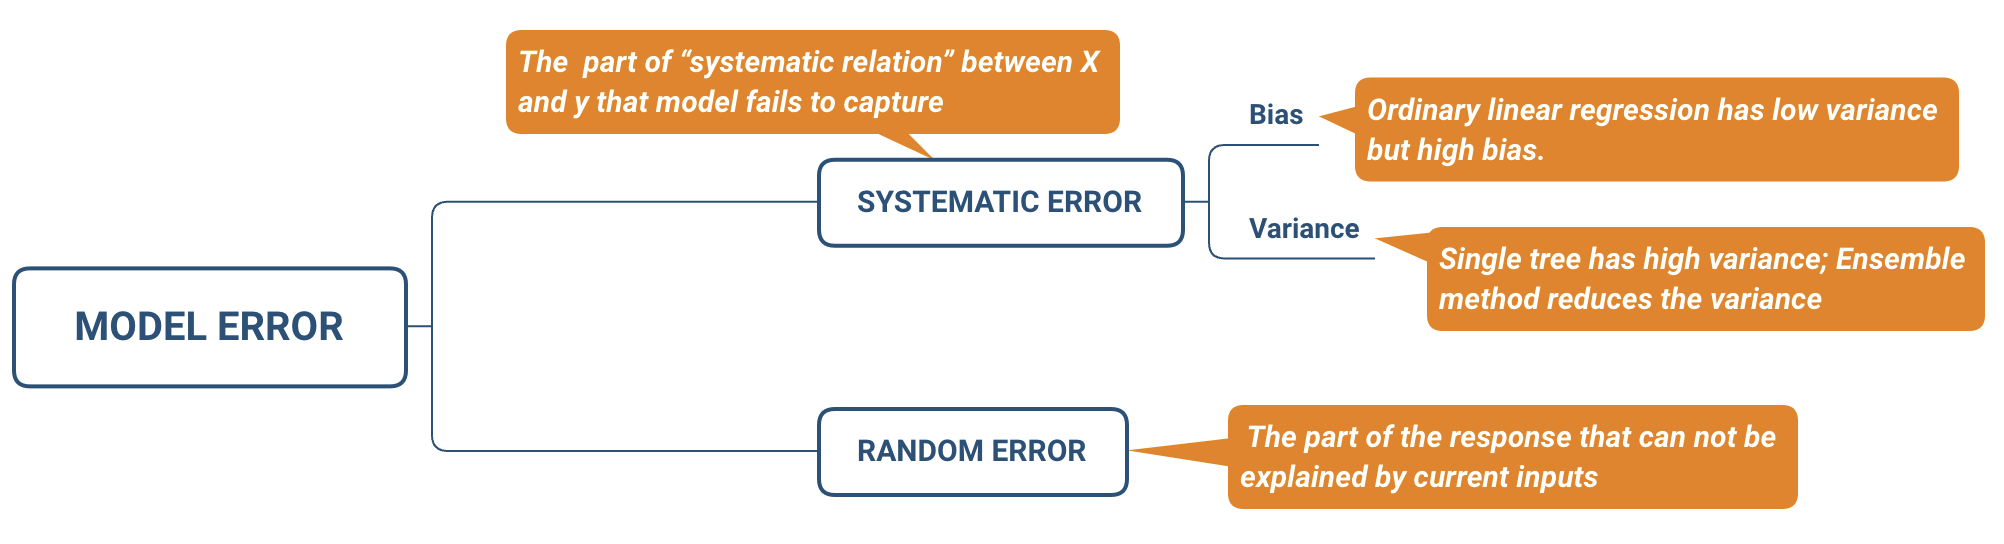
\includegraphics{images/ModelError.png}
\caption{Types of Model Error}
\end{figure}

The systematic error can be further decomposed as:

\[
\begin{array}{ccc}
E[f(\mathbf{X})-\hat{f}(\mathbf{X})]^{2} & = & E\left(f(\mathbf{X})-E[\hat{f}(\mathbf{X})]+E[\hat{f}(\mathbf{X})]-\hat{f}(\mathbf{X})\right)^{2}\\
 & = & E\left(E[\hat{f}(\mathbf{X})]-f(\mathbf{X})\right)^{2}+E\left(\hat{f}(\mathbf{X})-E[\hat{f}(\mathbf{X})]\right)^{2}\\
 & = & [Bias(\hat{f}(\mathbf{X}))]^{2}+Var(\hat{f}(\mathbf{X}))
\end{array}
\]

The systematic error consists of two parts,
\(Bias(\hat{f}(\mathbf{X}))\) and \(Var (\hat{f}(\mathbf{X}))\). To
minimize the systematic error, we need to minimize both. The bias
represents the error caused by the model's approximation of the reality,
i.e., systematic relation, which may be very complex. For example,
linear regression assumes a linear relationship between the predictors
and the response, but rarely is there a perfect linear relationship in
real life. So linear regression is more likely to have a high bias.

To explore bias and variance, let's begin with a simple simulation. We
will simulate a data with a non-linear relationship and fit different
models on it. An intuitive way to show these is to compare the plots of
various models.

The code below simulates one predictor (\texttt{x}) and one response
variable (\texttt{fx}). The relationship between \texttt{x} and
\texttt{fx} is non-linear.

\begin{Shaded}
\begin{Highlighting}[]
\KeywordTok{source}\NormalTok{(}\KeywordTok{ids_url}\NormalTok{(}\StringTok{'R/multiplot.r'}\NormalTok{))}
\CommentTok{# randomly simulate some non-linear samples}
\NormalTok{x =}\StringTok{ }\KeywordTok{seq}\NormalTok{(}\DecValTok{1}\NormalTok{, }\DecValTok{10}\NormalTok{, }\FloatTok{0.01}\NormalTok{) }\OperatorTok{*}\StringTok{ }\NormalTok{pi}
\NormalTok{e =}\StringTok{ }\KeywordTok{rnorm}\NormalTok{(}\KeywordTok{length}\NormalTok{(x), }\DataTypeTok{mean =} \DecValTok{0}\NormalTok{, }\DataTypeTok{sd =} \FloatTok{0.2}\NormalTok{)}
\NormalTok{fx <-}\StringTok{ }\KeywordTok{sin}\NormalTok{(x) }\OperatorTok{+}\StringTok{ }\NormalTok{e }\OperatorTok{+}\StringTok{ }\KeywordTok{sqrt}\NormalTok{(x)}
\NormalTok{dat =}\StringTok{ }\KeywordTok{data.frame}\NormalTok{(x, fx)}
\end{Highlighting}
\end{Shaded}

Then fit a simple linear regression on these data:

\begin{Shaded}
\begin{Highlighting}[]
\CommentTok{# plot fitting result}
\KeywordTok{library}\NormalTok{(ggplot2)}
\KeywordTok{ggplot}\NormalTok{(dat, }\KeywordTok{aes}\NormalTok{(x, fx)) }\OperatorTok{+}\StringTok{ }\KeywordTok{geom_point}\NormalTok{() }\OperatorTok{+}\StringTok{ }\KeywordTok{geom_smooth}\NormalTok{(}\DataTypeTok{method =} \StringTok{"lm"}\NormalTok{, }\DataTypeTok{se =} \OtherTok{FALSE}\NormalTok{)}
\end{Highlighting}
\end{Shaded}

\begin{figure}

{\centering 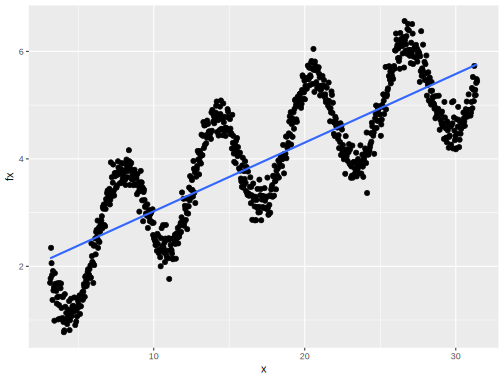
\includegraphics[width=0.8\linewidth]{IDS_files/figure-latex/linearbias-1} 

}

\caption{High bias model}\label{fig:linearbias}
\end{figure}

Despite a large sample size, trained linear regression cannot describe
the relationship very well. In other words, in this case, the model has
a high bias (Fig. \ref{fig:linearbias}). People also call it
underfitting.

Since the estimated parameters will be somewhat different for different
samples, there is the variance of estimates. Intuitively, it gives you
some sense that if we fit the same model with different samples
(presumably, they are from the same population), how much will the
estimates change. Ideally, the change is trivial. For high variance
models, small changes in the training data result in very different
estimates. In general, a model with high flexibility also has high
variance., such as the CART tree, and the initial boosting method. To
overcome that problem, the Random Forest and Gradient Boosting Model aim
to reduce the variance by summarizing the results obtained from
different samples.

Let's fit the above data using a smoothing method which is highly
flexible and can fit the current data tightly:

\begin{Shaded}
\begin{Highlighting}[]
\KeywordTok{ggplot}\NormalTok{(dat, }\KeywordTok{aes}\NormalTok{(x, fx)) }\OperatorTok{+}\StringTok{ }\KeywordTok{geom_smooth}\NormalTok{(}\DataTypeTok{span =} \FloatTok{0.03}\NormalTok{)}
\end{Highlighting}
\end{Shaded}

\begin{figure}

{\centering 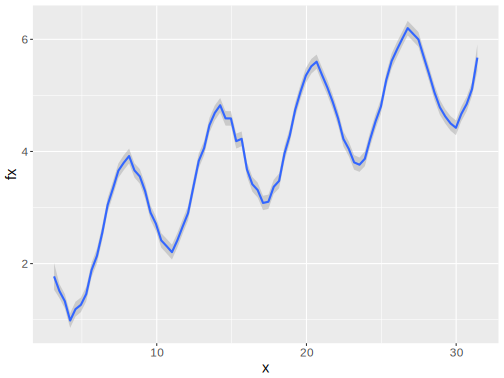
\includegraphics[width=0.8\linewidth]{IDS_files/figure-latex/linearvar-1} 

}

\caption{High variance model}\label{fig:linearvar}
\end{figure}

The resulting plot (Fig. \ref{fig:linearvar}) indicates the smoothing
method fit the data much better so it has a much smaller bias. However,
this method has a high variance. If we simulate different subsets of the
sample, the result curve will change significantly:

\begin{Shaded}
\begin{Highlighting}[]
\CommentTok{# set random seed}
\KeywordTok{set.seed}\NormalTok{(}\DecValTok{2016}\NormalTok{)}
\CommentTok{# sample part of the data to fit model sample 1}
\NormalTok{idx1 =}\StringTok{ }\KeywordTok{sample}\NormalTok{(}\DecValTok{1}\OperatorTok{:}\KeywordTok{length}\NormalTok{(x), }\DecValTok{100}\NormalTok{)}
\NormalTok{dat1 =}\StringTok{ }\KeywordTok{data.frame}\NormalTok{(}\DataTypeTok{x1 =}\NormalTok{ x[idx1], }\DataTypeTok{fx1 =}\NormalTok{ fx[idx1])}
\NormalTok{p1 =}\StringTok{ }\KeywordTok{ggplot}\NormalTok{(dat1, }\KeywordTok{aes}\NormalTok{(x1, fx1)) }\OperatorTok{+}\StringTok{ }\KeywordTok{geom_smooth}\NormalTok{(}\DataTypeTok{span =} \FloatTok{0.03}\NormalTok{)}
\CommentTok{# sample 2}
\NormalTok{idx2 =}\StringTok{ }\KeywordTok{sample}\NormalTok{(}\DecValTok{1}\OperatorTok{:}\KeywordTok{length}\NormalTok{(x), }\DecValTok{100}\NormalTok{)}
\NormalTok{dat2 =}\StringTok{ }\KeywordTok{data.frame}\NormalTok{(}\DataTypeTok{x2 =}\NormalTok{ x[idx2], }\DataTypeTok{fx2 =}\NormalTok{ fx[idx2])}
\NormalTok{p2 =}\StringTok{ }\KeywordTok{ggplot}\NormalTok{(dat2, }\KeywordTok{aes}\NormalTok{(x2, fx2)) }\OperatorTok{+}\StringTok{ }\KeywordTok{geom_smooth}\NormalTok{(}\DataTypeTok{span =} \FloatTok{0.03}\NormalTok{)}
\CommentTok{# sample 3}
\NormalTok{idx3 =}\StringTok{ }\KeywordTok{sample}\NormalTok{(}\DecValTok{1}\OperatorTok{:}\KeywordTok{length}\NormalTok{(x), }\DecValTok{100}\NormalTok{)}
\NormalTok{dat3 =}\StringTok{ }\KeywordTok{data.frame}\NormalTok{(}\DataTypeTok{x3 =}\NormalTok{ x[idx3], }\DataTypeTok{fx3 =}\NormalTok{ fx[idx3])}
\NormalTok{p3 =}\StringTok{ }\KeywordTok{ggplot}\NormalTok{(dat3, }\KeywordTok{aes}\NormalTok{(x3, fx3)) }\OperatorTok{+}\StringTok{ }\KeywordTok{geom_smooth}\NormalTok{(}\DataTypeTok{span =} \FloatTok{0.03}\NormalTok{)}
\CommentTok{# sample 4}
\NormalTok{idx4 =}\StringTok{ }\KeywordTok{sample}\NormalTok{(}\DecValTok{1}\OperatorTok{:}\KeywordTok{length}\NormalTok{(x), }\DecValTok{100}\NormalTok{)}
\NormalTok{dat4 =}\StringTok{ }\KeywordTok{data.frame}\NormalTok{(}\DataTypeTok{x4 =}\NormalTok{ x[idx4], }\DataTypeTok{fx4 =}\NormalTok{ fx[idx4])}
\NormalTok{p4 =}\StringTok{ }\KeywordTok{ggplot}\NormalTok{(dat4, }\KeywordTok{aes}\NormalTok{(x4, fx4)) }\OperatorTok{+}\StringTok{ }\KeywordTok{geom_smooth}\NormalTok{(}\DataTypeTok{span =} \FloatTok{0.03}\NormalTok{)}
\KeywordTok{multiplot}\NormalTok{(p1, p2, p3, p4, }\DataTypeTok{cols =} \DecValTok{2}\NormalTok{)}
\end{Highlighting}
\end{Shaded}

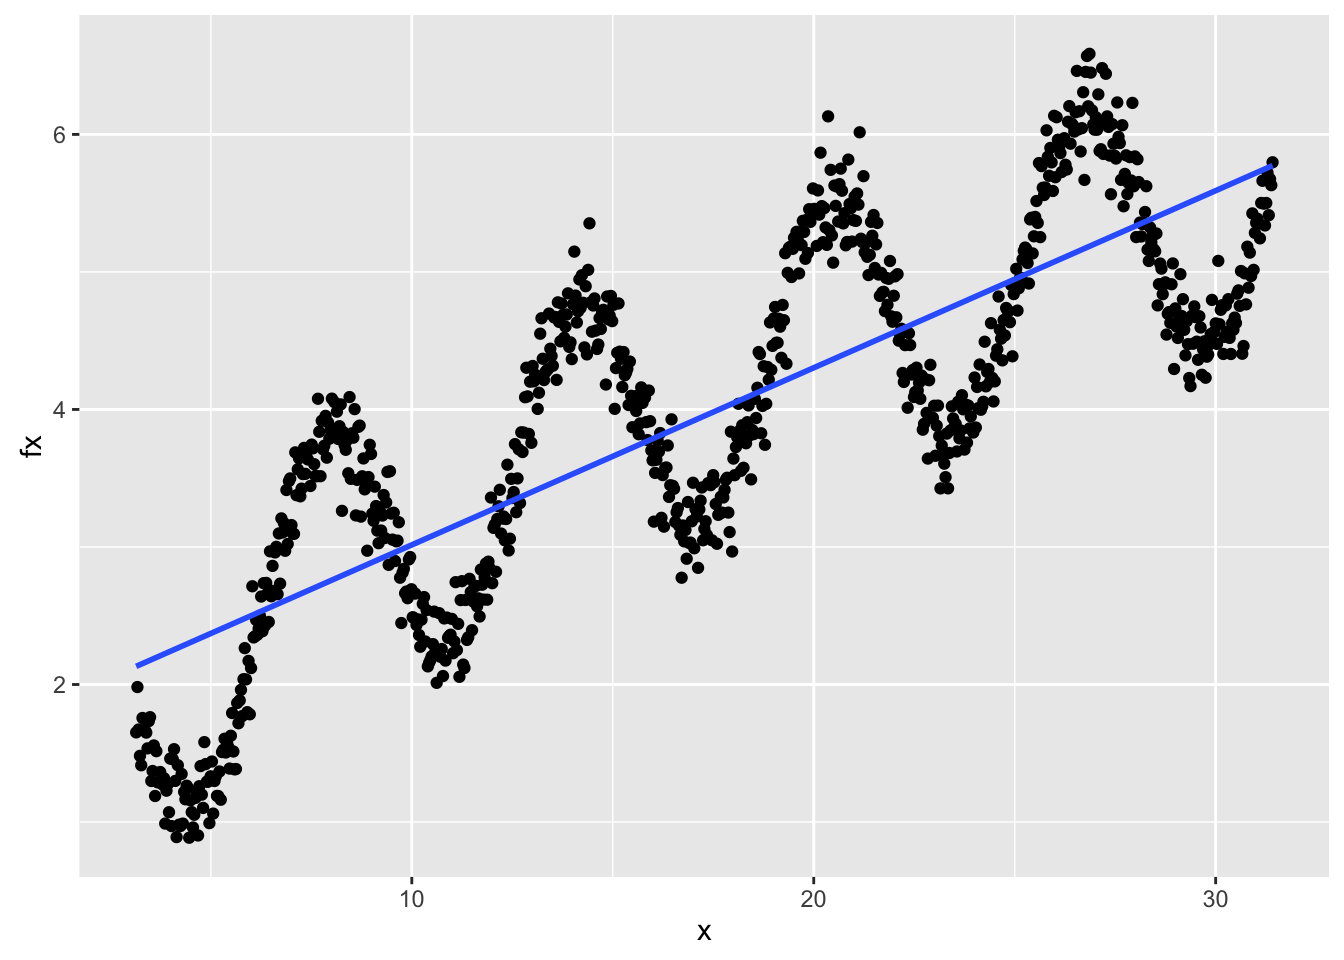
\includegraphics{IDS_files/figure-latex/unnamed-chunk-66-1.pdf}

The fitted lines (blue) change over different samples which means it has
high variance. People also call it overfitting. Fitting the linear model
using the same four subsets, the result barely changes:

\begin{Shaded}
\begin{Highlighting}[]
\NormalTok{p1 =}\StringTok{ }\KeywordTok{ggplot}\NormalTok{(dat1, }\KeywordTok{aes}\NormalTok{(x1, fx1)) }\OperatorTok{+}\StringTok{ }\KeywordTok{geom_point}\NormalTok{() }\OperatorTok{+}\StringTok{ }\KeywordTok{geom_smooth}\NormalTok{(}\DataTypeTok{method =} \StringTok{"lm"}\NormalTok{, }
    \DataTypeTok{se =} \OtherTok{FALSE}\NormalTok{)}
\NormalTok{p2 =}\StringTok{ }\KeywordTok{ggplot}\NormalTok{(dat2, }\KeywordTok{aes}\NormalTok{(x2, fx2)) }\OperatorTok{+}\StringTok{ }\KeywordTok{geom_point}\NormalTok{() }\OperatorTok{+}\StringTok{ }\KeywordTok{geom_smooth}\NormalTok{(}\DataTypeTok{method =} \StringTok{"lm"}\NormalTok{, }
    \DataTypeTok{se =} \OtherTok{FALSE}\NormalTok{)}
\NormalTok{p3 =}\StringTok{ }\KeywordTok{ggplot}\NormalTok{(dat3, }\KeywordTok{aes}\NormalTok{(x3, fx3)) }\OperatorTok{+}\StringTok{ }\KeywordTok{geom_point}\NormalTok{() }\OperatorTok{+}\StringTok{ }\KeywordTok{geom_smooth}\NormalTok{(}\DataTypeTok{method =} \StringTok{"lm"}\NormalTok{, }
    \DataTypeTok{se =} \OtherTok{FALSE}\NormalTok{)}
\NormalTok{p4 =}\StringTok{ }\KeywordTok{ggplot}\NormalTok{(dat4, }\KeywordTok{aes}\NormalTok{(x4, fx4)) }\OperatorTok{+}\StringTok{ }\KeywordTok{geom_point}\NormalTok{() }\OperatorTok{+}\StringTok{ }\KeywordTok{geom_smooth}\NormalTok{(}\DataTypeTok{method =} \StringTok{"lm"}\NormalTok{, }
    \DataTypeTok{se =} \OtherTok{FALSE}\NormalTok{)}
\KeywordTok{multiplot}\NormalTok{(p1, p2, p3, p4, }\DataTypeTok{cols =} \DecValTok{2}\NormalTok{)}
\end{Highlighting}
\end{Shaded}

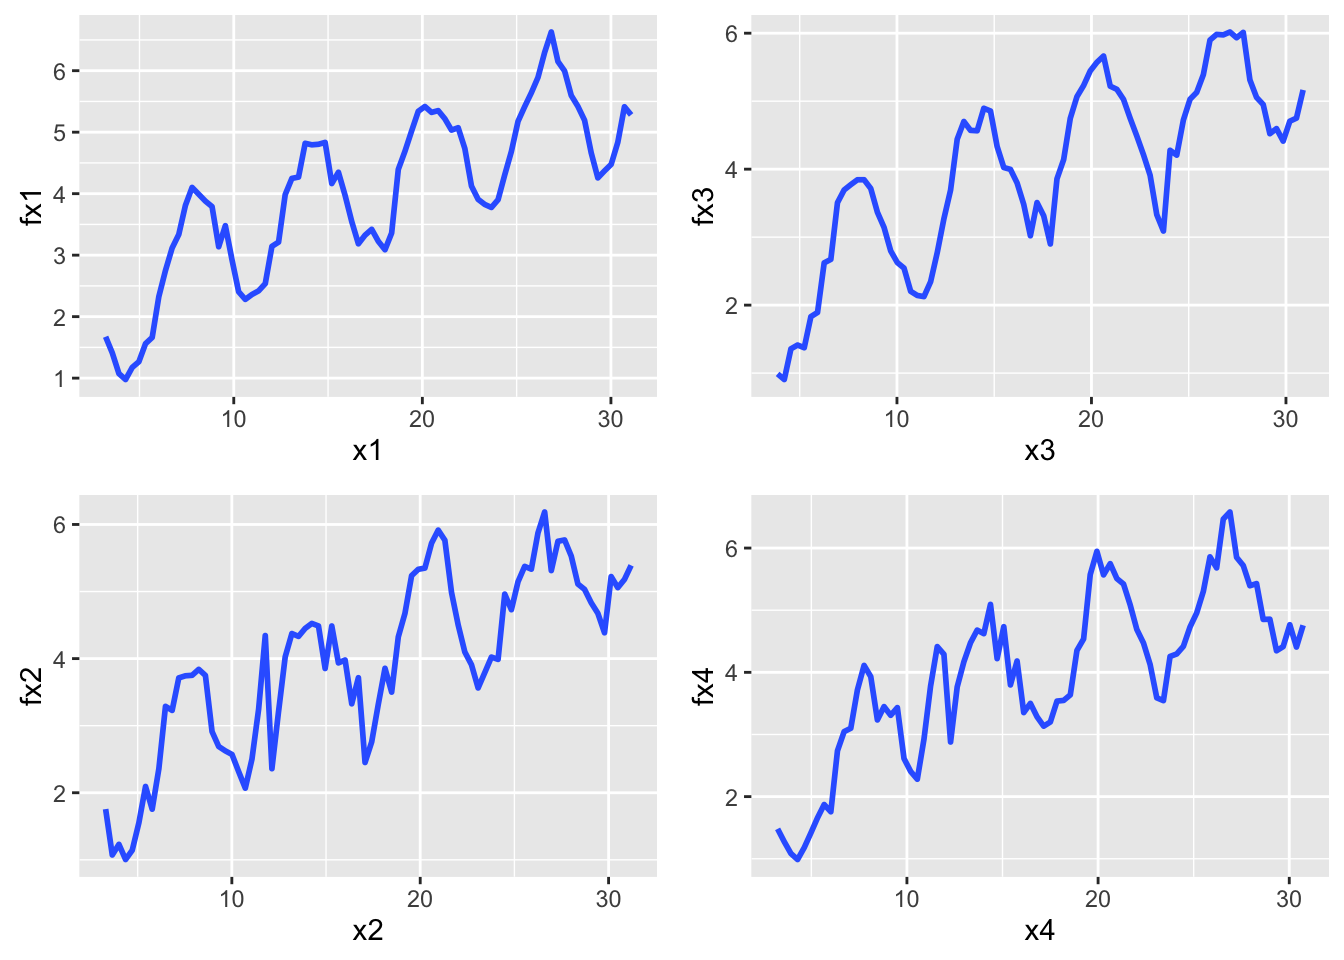
\includegraphics{IDS_files/figure-latex/unnamed-chunk-67-1.pdf}

In general, the variance (\(Var(\hat{f}(\mathbf{X}))\))
\textbf{increases} and the bias (\(Bias(\hat{f}(\mathbf{X}))\))
\textbf{decreases} as the model flexibility increases. Variance and bias
together determine the systematic error. As we increase the flexibility
of the model, at first the rate at which \(Bias(\hat{f}(\mathbf{X}))\)
decreases is faster than \(Var (\hat{f} (\mathbf{X}))\), so the MSE
decreases. However, to some degree, higher flexibility has little effect
on \(Bias(\hat{f}(\mathbf{X}))\) but \(Var(\hat{f} (\mathbf{X}))\)
increases significantly, so the MSE increases.

\subsection{Measurement Error in the
Response}\label{measurement-error-in-the-response}

The measurement error in the response contributes to the random error
(\(\mathbf{\epsilon}\)). This part of the error is irreducible if you
change the data collection mechanism, and so it makes the root mean
square error (RMSE) and \(R^2\) have the corresponding upper and lower
limits. RMSE and \(R^2\) are commonly used performance measures for the
regression model which we will talk in more detail later. Therefore, the
random error term not only represents the part of fluctuations the model
cannot explain but also contains measurement error in the response
variables. Section 20.2 of Applied Predictive Modeling \citep{APM} has
an example that shows the effect of the measurement error in the
response variable on the model performance (RMSE and \(R^2\)).

The authors increased the error in the response proportional to a base
level error which was gotten using the original data without introducing
extra noise. Then fit a set of models repeatedly using the
``contaminated'' data sets to study the change of \(RMSE\) and \(R^2\)
as the level of noise. Here we use clothing consumer data for a similar
illustration. Suppose many people do not want to disclose their income
and so we need to use other variables to establish a model to predict
income. We set up the following model:

\begin{Shaded}
\begin{Highlighting}[]
\CommentTok{# load data}
\NormalTok{sim.dat <-}\StringTok{ }\KeywordTok{read.csv}\NormalTok{(}\StringTok{"http://bit.ly/2P5gTw4"}\NormalTok{)}
\NormalTok{ymad <-}\StringTok{ }\KeywordTok{mad}\NormalTok{(}\KeywordTok{na.omit}\NormalTok{(sim.dat}\OperatorTok{$}\NormalTok{income))}
\CommentTok{# calculate z-score}
\NormalTok{zs <-}\StringTok{ }\NormalTok{(sim.dat}\OperatorTok{$}\NormalTok{income }\OperatorTok{-}\StringTok{ }\KeywordTok{mean}\NormalTok{(}\KeywordTok{na.omit}\NormalTok{(sim.dat}\OperatorTok{$}\NormalTok{income)))}\OperatorTok{/}\NormalTok{ymad}
\CommentTok{# which(na.omit(zs>3.5)): identify outliers which(is.na(zs)):}
\CommentTok{# identify missing values}
\NormalTok{idex <-}\StringTok{ }\KeywordTok{c}\NormalTok{(}\KeywordTok{which}\NormalTok{(}\KeywordTok{na.omit}\NormalTok{(zs }\OperatorTok{>}\StringTok{ }\FloatTok{3.5}\NormalTok{)), }\KeywordTok{which}\NormalTok{(}\KeywordTok{is.na}\NormalTok{(zs)))}
\CommentTok{# delete rows with outliers and missing values}
\NormalTok{sim.dat <-}\StringTok{ }\NormalTok{sim.dat[}\OperatorTok{-}\NormalTok{idex, ]}
\NormalTok{fit <-}\StringTok{ }\KeywordTok{lm}\NormalTok{(income }\OperatorTok{~}\StringTok{ }\NormalTok{store_exp }\OperatorTok{+}\StringTok{ }\NormalTok{online_exp }\OperatorTok{+}\StringTok{ }\NormalTok{store_trans }\OperatorTok{+}\StringTok{ }\NormalTok{online_trans, }
    \DataTypeTok{data =}\NormalTok{ sim.dat)}
\end{Highlighting}
\end{Shaded}

The output shows that without additional noise, the root mean square
error (RMSE) of the model is 29567, \(R^2\) is 0.6.

Let's add various degrees of noise (0 to 3 times the RMSE) to the
variable \texttt{income}:

\[ RMSE \times (0.0, 0.5, 1.0, 1.5, 2.0, 2.5, 3.0) \]

\begin{Shaded}
\begin{Highlighting}[]
\NormalTok{noise <-}\StringTok{ }\KeywordTok{matrix}\NormalTok{(}\KeywordTok{rep}\NormalTok{(}\OtherTok{NA}\NormalTok{, }\DecValTok{7} \OperatorTok{*}\StringTok{ }\KeywordTok{nrow}\NormalTok{(sim.dat)), }\DataTypeTok{nrow =} \KeywordTok{nrow}\NormalTok{(sim.dat), }
    \DataTypeTok{ncol =} \DecValTok{7}\NormalTok{)}
\ControlFlowTok{for}\NormalTok{ (i }\ControlFlowTok{in} \DecValTok{1}\OperatorTok{:}\KeywordTok{nrow}\NormalTok{(sim.dat)) \{}
\NormalTok{    noise[i, ] <-}\StringTok{ }\KeywordTok{rnorm}\NormalTok{(}\DecValTok{7}\NormalTok{, }\KeywordTok{rep}\NormalTok{(}\DecValTok{0}\NormalTok{, }\DecValTok{7}\NormalTok{), }\KeywordTok{summary}\NormalTok{(fit)}\OperatorTok{$}\NormalTok{sigma }\OperatorTok{*}\StringTok{ }\KeywordTok{seq}\NormalTok{(}\DecValTok{0}\NormalTok{, }
        \DecValTok{3}\NormalTok{, }\DataTypeTok{by =} \FloatTok{0.5}\NormalTok{))}
\NormalTok{\}}
\end{Highlighting}
\end{Shaded}

We then examine the effect of noise intensity on \(R^2\) for models with
different complexity. The models with complexity from low to high are:
ordinary linear regression, partial least square regression(PLS),
multivariate adaptive regression spline (MARS), support vector machine
(SVM, the kernel function is radial basis function), and random forest.

\begin{Shaded}
\begin{Highlighting}[]
\CommentTok{# fit ordinary linear regression}
\NormalTok{rsq_linear <-}\StringTok{ }\KeywordTok{rep}\NormalTok{(}\DecValTok{0}\NormalTok{, }\KeywordTok{ncol}\NormalTok{(noise))}
\ControlFlowTok{for}\NormalTok{ (i }\ControlFlowTok{in} \DecValTok{1}\OperatorTok{:}\DecValTok{7}\NormalTok{) \{}
\NormalTok{    withnoise <-}\StringTok{ }\NormalTok{sim.dat}\OperatorTok{$}\NormalTok{income }\OperatorTok{+}\StringTok{ }\NormalTok{noise[, i]}
\NormalTok{    fit0 <-}\StringTok{ }\KeywordTok{lm}\NormalTok{(withnoise }\OperatorTok{~}\StringTok{ }\NormalTok{store_exp }\OperatorTok{+}\StringTok{ }\NormalTok{online_exp }\OperatorTok{+}\StringTok{ }\NormalTok{store_trans }\OperatorTok{+}\StringTok{ }
\StringTok{        }\NormalTok{online_trans, }\DataTypeTok{data =}\NormalTok{ sim.dat)}
\NormalTok{    rsq_linear[i] <-}\StringTok{ }\KeywordTok{summary}\NormalTok{(fit0)}\OperatorTok{$}\NormalTok{adj.r.squared}
\NormalTok{\}}
\end{Highlighting}
\end{Shaded}

PLS is a method of linearizing nonlinear relationships through hidden
layers. It is similar to the principal component regression (PCR),
except that PCR does not take into account the information of the
dependent variable when selecting the components, and its purpose is to
find the linear combinations (i.e., unsupervised) that capture the most
variance of the independent variables. When the independent variables
and response variables are related, PCR can well identify the systematic
relationship between them. However, when there exist independent
variables not associated with response variable, it will undermine PCR's
performance. And PLS maximizes the linear combination of dependencies
with the response variable. In the current case, the more complicated
PLS does not perform better than simple linear regression.

\begin{Shaded}
\begin{Highlighting}[]
\CommentTok{# pls: conduct PLS and PCR}
\KeywordTok{library}\NormalTok{(pls)}
\NormalTok{rsq_pls <-}\StringTok{ }\KeywordTok{rep}\NormalTok{(}\DecValTok{0}\NormalTok{, }\KeywordTok{ncol}\NormalTok{(noise))}
\CommentTok{# fit PLS}
\ControlFlowTok{for}\NormalTok{ (i }\ControlFlowTok{in} \DecValTok{1}\OperatorTok{:}\DecValTok{7}\NormalTok{) \{}
\NormalTok{    withnoise <-}\StringTok{ }\NormalTok{sim.dat}\OperatorTok{$}\NormalTok{income }\OperatorTok{+}\StringTok{ }\NormalTok{noise[, i]}
\NormalTok{    fit0 <-}\StringTok{ }\KeywordTok{plsr}\NormalTok{(withnoise }\OperatorTok{~}\StringTok{ }\NormalTok{store_exp }\OperatorTok{+}\StringTok{ }\NormalTok{online_exp }\OperatorTok{+}\StringTok{ }\NormalTok{store_trans }\OperatorTok{+}\StringTok{ }
\StringTok{        }\NormalTok{online_trans, }\DataTypeTok{data =}\NormalTok{ sim.dat)}
\NormalTok{    rsq_pls[i] <-}\StringTok{ }\KeywordTok{max}\NormalTok{(}\KeywordTok{drop}\NormalTok{(}\KeywordTok{R2}\NormalTok{(fit0, }\DataTypeTok{estimate =} \StringTok{"train"}\NormalTok{, }\DataTypeTok{intercept =} \OtherTok{FALSE}\NormalTok{)}\OperatorTok{$}\NormalTok{val))}
\NormalTok{\}}
\end{Highlighting}
\end{Shaded}

\begin{Shaded}
\begin{Highlighting}[]
\CommentTok{# earth: fit mars}
\KeywordTok{library}\NormalTok{(earth)}
\NormalTok{rsq_mars <-}\StringTok{ }\KeywordTok{rep}\NormalTok{(}\DecValTok{0}\NormalTok{, }\KeywordTok{ncol}\NormalTok{(noise))}
\ControlFlowTok{for}\NormalTok{ (i }\ControlFlowTok{in} \DecValTok{1}\OperatorTok{:}\DecValTok{7}\NormalTok{) \{}
\NormalTok{    withnoise <-}\StringTok{ }\NormalTok{sim.dat}\OperatorTok{$}\NormalTok{income }\OperatorTok{+}\StringTok{ }\NormalTok{noise[, i]}
\NormalTok{    fit0 <-}\StringTok{ }\KeywordTok{earth}\NormalTok{(withnoise }\OperatorTok{~}\StringTok{ }\NormalTok{store_exp }\OperatorTok{+}\StringTok{ }\NormalTok{online_exp }\OperatorTok{+}\StringTok{ }\NormalTok{store_trans }\OperatorTok{+}\StringTok{ }
\StringTok{        }\NormalTok{online_trans, }\DataTypeTok{data =}\NormalTok{ sim.dat)}
\NormalTok{    rsq_mars[i] <-}\StringTok{ }\NormalTok{fit0}\OperatorTok{$}\NormalTok{rsq}
\NormalTok{\}}
\end{Highlighting}
\end{Shaded}

\begin{Shaded}
\begin{Highlighting}[]
\CommentTok{# caret: awesome package for tuning predictive model}
\KeywordTok{library}\NormalTok{(caret)}
\NormalTok{rsq_svm <-}\StringTok{ }\KeywordTok{rep}\NormalTok{(}\DecValTok{0}\NormalTok{, }\KeywordTok{ncol}\NormalTok{(noise))}
\CommentTok{# Need some time to run}
\ControlFlowTok{for}\NormalTok{ (i }\ControlFlowTok{in} \DecValTok{1}\OperatorTok{:}\DecValTok{7}\NormalTok{) \{}
\NormalTok{    idex <-}\StringTok{ }\KeywordTok{which}\NormalTok{(}\KeywordTok{is.na}\NormalTok{(sim.dat}\OperatorTok{$}\NormalTok{income))}
\NormalTok{    withnoise <-}\StringTok{ }\NormalTok{sim.dat}\OperatorTok{$}\NormalTok{income }\OperatorTok{+}\StringTok{ }\NormalTok{noise[, i]}
\NormalTok{    trainX <-}\StringTok{ }\NormalTok{sim.dat[, }\KeywordTok{c}\NormalTok{(}\StringTok{"store_exp"}\NormalTok{, }\StringTok{"online_exp"}\NormalTok{, }\StringTok{"store_trans"}\NormalTok{, }
        \StringTok{"online_trans"}\NormalTok{)]}
\NormalTok{    trainY <-}\StringTok{ }\NormalTok{withnoise}
\NormalTok{    fit0 <-}\StringTok{ }\KeywordTok{train}\NormalTok{(trainX, trainY, }\DataTypeTok{method =} \StringTok{"svmRadial"}\NormalTok{, }\DataTypeTok{tuneLength =} \DecValTok{15}\NormalTok{, }
        \DataTypeTok{trControl =} \KeywordTok{trainControl}\NormalTok{(}\DataTypeTok{method =} \StringTok{"cv"}\NormalTok{))}
\NormalTok{    rsq_svm[i] <-}\StringTok{ }\KeywordTok{max}\NormalTok{(fit0}\OperatorTok{$}\NormalTok{results}\OperatorTok{$}\NormalTok{Rsquared)}
\NormalTok{\}}
\end{Highlighting}
\end{Shaded}

\begin{Shaded}
\begin{Highlighting}[]
\CommentTok{# randomForest: random forest model}
\KeywordTok{library}\NormalTok{(randomForest)}
\NormalTok{rsq_rf <-}\StringTok{ }\KeywordTok{rep}\NormalTok{(}\DecValTok{0}\NormalTok{, }\KeywordTok{ncol}\NormalTok{(noise))}
\CommentTok{# ntree=500 number of trees na.action = na.omit ignore}
\CommentTok{# missing value}
\ControlFlowTok{for}\NormalTok{ (i }\ControlFlowTok{in} \DecValTok{1}\OperatorTok{:}\DecValTok{7}\NormalTok{) \{}
\NormalTok{    withnoise <-}\StringTok{ }\NormalTok{sim.dat}\OperatorTok{$}\NormalTok{income }\OperatorTok{+}\StringTok{ }\NormalTok{noise[, i]}
\NormalTok{    fit0 <-}\StringTok{ }\KeywordTok{randomForest}\NormalTok{(withnoise }\OperatorTok{~}\StringTok{ }\NormalTok{store_exp }\OperatorTok{+}\StringTok{ }\NormalTok{online_exp }\OperatorTok{+}\StringTok{ }
\StringTok{        }\NormalTok{store_trans }\OperatorTok{+}\StringTok{ }\NormalTok{online_trans, }\DataTypeTok{data =}\NormalTok{ sim.dat, }\DataTypeTok{ntree =} \DecValTok{500}\NormalTok{, }
        \DataTypeTok{na.action =}\NormalTok{ na.omit)}
\NormalTok{    rsq_rf[i] <-}\StringTok{ }\KeywordTok{tail}\NormalTok{(fit0}\OperatorTok{$}\NormalTok{rsq, }\DecValTok{1}\NormalTok{)}
\NormalTok{\}}
\KeywordTok{library}\NormalTok{(reshape2)}
\NormalTok{rsq <-}\StringTok{ }\KeywordTok{data.frame}\NormalTok{(}\KeywordTok{cbind}\NormalTok{(}\DataTypeTok{Noise =} \KeywordTok{c}\NormalTok{(}\DecValTok{0}\NormalTok{, }\FloatTok{0.5}\NormalTok{, }\DecValTok{1}\NormalTok{, }\FloatTok{1.5}\NormalTok{, }\DecValTok{2}\NormalTok{, }\FloatTok{2.5}\NormalTok{, }\DecValTok{3}\NormalTok{), }
\NormalTok{    rsq_linear, rsq_pls, rsq_mars, rsq_svm, rsq_rf))}
\NormalTok{rsq <-}\StringTok{ }\KeywordTok{melt}\NormalTok{(rsq, }\DataTypeTok{id.vars =} \StringTok{"Noise"}\NormalTok{, }\DataTypeTok{measure.vars =} \KeywordTok{c}\NormalTok{(}\StringTok{"rsq_linear"}\NormalTok{, }
    \StringTok{"rsq_pls"}\NormalTok{, }\StringTok{"rsq_mars"}\NormalTok{, }\StringTok{"rsq_svm"}\NormalTok{, }\StringTok{"rsq_rf"}\NormalTok{))}
\end{Highlighting}
\end{Shaded}







\begin{Shaded}
\begin{Highlighting}[]
\KeywordTok{library}\NormalTok{(ggplot2)}
\KeywordTok{ggplot}\NormalTok{(}\DataTypeTok{data =}\NormalTok{ rsq, }\KeywordTok{aes}\NormalTok{(}\DataTypeTok{x =}\NormalTok{ Noise, }\DataTypeTok{y =}\NormalTok{ value, }\DataTypeTok{group =}\NormalTok{ variable, }
    \DataTypeTok{colour =}\NormalTok{ variable)) }\OperatorTok{+}\StringTok{ }\KeywordTok{geom_line}\NormalTok{() }\OperatorTok{+}\StringTok{ }\KeywordTok{geom_point}\NormalTok{() }\OperatorTok{+}\StringTok{ }\KeywordTok{ylab}\NormalTok{(}\StringTok{"R2"}\NormalTok{)}
\end{Highlighting}
\end{Shaded}

\begin{figure}

{\centering 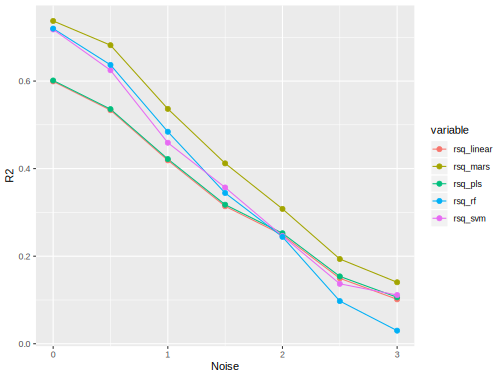
\includegraphics[width=0.8\linewidth]{IDS_files/figure-latex/error-1} 

}

\caption{Test set \(R^2\) profiles for income models when
measurement system noise increases. \texttt{rsq\_linear}: linear
regression, \texttt{rsq\_pls}: Partial Least Square, \texttt{rsq\_mars}:
Multiple Adaptive Regression Spline Regression, \texttt{rsq\_svm}:
Support Vector Machine,\texttt{rsq\_rf}: Random Forest}\label{fig:error}
\end{figure}

Fig. \ref{fig:error} shows that:

All model performance decreases sharply with increasing noise intensity.
To better anticipate model performance, it helps to understand the way
variable is measured. It is something need to make clear at the
beginning of an analytical project. A data scientist should be aware of
the quality of the data in the database. For data from the clients, it
is an important to understand the quality of the data by communication.

More complex model is not necessarily better. The best model in this
situation is MARS, not random forests or SVM. Simple linear regression
and PLS perform the worst when noise is low. MARS is more complicated
than the linear regression and PLS, but it is simpler and easier to
explain than random forest and SVM.

When noise increases to a certain extent, the potential structure
becomes vaguer, and complex random forest model starts to fail. When the
systematic measurement error is significant, a more straightforward but
not naive model may be a better choice. It is always a good practice to
try different models, and select the simplest model in the case of
similar performance. Model evaluation and selection represent the career
``maturity'' of a data scientist.

\subsection{Measurement Error in the Independent
Variables}\label{measurement-error-in-the-independent-variables}

The traditional statistical model usually assumes that the measurement
of the independent variable has no error which is not possible in
practice. Considering the error in the independent variables is
necessary. The impact of the error depends on the following factors: (1)
the magnitude of the randomness; (2) the importance of the corresponding
variable in the model, and (3) the type of model used. Use variable
\texttt{online\_exp} as an example. The approach is similar to the
previous section. Add varying degrees of noise and see its impact on the
model performance. We add the following different levels of noise (0 to
3 times the standard deviation) to\texttt{online\_exp}:

\[\sigma_{0} \times (0.0, 0.5, 1.0, 1.5, 2.0, 2.5, 3.0)\]

where \(\sigma_{0}\) is the standard error of \texttt{online\_exp}.

\begin{Shaded}
\begin{Highlighting}[]
\NormalTok{noise<-}\KeywordTok{matrix}\NormalTok{(}\KeywordTok{rep}\NormalTok{(}\OtherTok{NA}\NormalTok{,}\DecValTok{7}\OperatorTok{*}\KeywordTok{nrow}\NormalTok{(sim.dat)),}\DataTypeTok{nrow=}\KeywordTok{nrow}\NormalTok{(sim.dat),}\DataTypeTok{ncol=}\DecValTok{7}\NormalTok{)}
\ControlFlowTok{for}\NormalTok{ (i }\ControlFlowTok{in} \DecValTok{1}\OperatorTok{:}\KeywordTok{nrow}\NormalTok{(sim.dat))\{}
\NormalTok{noise[i,]<-}\KeywordTok{rnorm}\NormalTok{(}\DecValTok{7}\NormalTok{,}\KeywordTok{rep}\NormalTok{(}\DecValTok{0}\NormalTok{,}\DecValTok{7}\NormalTok{),}\KeywordTok{sd}\NormalTok{(sim.dat}\OperatorTok{$}\NormalTok{online_exp)}\OperatorTok{*}\KeywordTok{seq}\NormalTok{(}\DecValTok{0}\NormalTok{,}\DecValTok{3}\NormalTok{,}\DataTypeTok{by=}\FloatTok{0.5}\NormalTok{))}
\NormalTok{\}}
\end{Highlighting}
\end{Shaded}

Likewise, we examine the effect of noise intensity on different models
(\(R^2\)). The models with complexity from low to high are: ordinary
linear regression, partial least square regression(PLS), multivariate
adaptive regression spline (MARS), support vector machine (SVM, the
Kernel function is radial basis function), and random forest. The code
is similar as before so not shown here.








\begin{figure}

{\centering 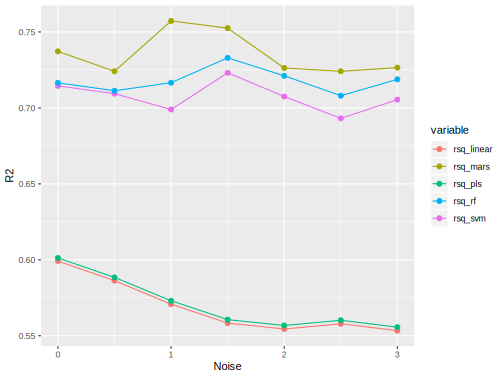
\includegraphics[width=0.8\linewidth]{IDS_files/figure-latex/errorvariable-1} 

}

\caption{Test set \(R^2\) profiles for income models when
noise in \texttt{online\_exp} increases. \texttt{rsq\_linear} : linear
regression, \texttt{rsq\_pls} : Partial Least Square,
\texttt{rsq\_mars}: Multiple Adaptive Regression Spline Regression,
\texttt{rsq\_svm}: Support Vector Machine,\texttt{rsq\_rf}: Random
Forest}\label{fig:errorvariable}
\end{figure}

Comparing Fig. \ref{fig:errorvariable} and Fig. \ref{fig:error}, the
influence of the two types of error is very different. The error in
response cannot be overcome for any model, but it is not the case for
the independent variables. Imagine an extreme case, if
\texttt{online\_exp} is completely random, that is, no information in
it, the impact on the performance of random forest and support vector
machine is marginal. Linear regression and PLS still perform similarly.
With the increase of noise, the performance starts to decline faster. To
a certain extent, it becomes steady. In general, if an independent
variable contains error, other variables associated with it can
compensate to some extent.

\section{Data Splitting and
Resampling}\label{data-splitting-and-resampling}

Those highly adaptable models can model complex relationships. However,
they tend to overfit which leads to the poor prediction by learning too
much from the data. It means that the model is susceptible to the
specific sample used to fit it. When future data is not exactly like the
past data, the model prediction may have big mistakes. A simple model
like ordinary linear regression tends instead to underfit which leads to
a bad prediction by learning too little from the data. It systematically
over-predicts or under-predicts the data regardless of how well future
data resemble past data. Without evaluating models, the modeler will not
know about the problem before the future samples. Data splitting and
resampling are fundamental techniques to build sound models for
prediction.

\subsection{Data Splitting}\label{data-splitting}

\emph{Data splitting} is to put part of the data aside as testing set
(or Hold-outs, out of bag samples) and use the rest for model training.
Training samples are also called in-sample. Model performance metrics
evaluated using in-sample are retrodictive, not predictive.

The traditional business intelligence usually handles data description.
Answer simple questions by querying and summarizing the data, such as:

\begin{itemize}
\tightlist
\item
  What is the monthly sales of a product in 2015?
\item
  What is the number of visits to our site in the past month?\\
\item
  What is the sales difference in 2015 for two different product
  designs?
\end{itemize}

There is no need to go through the tedious process of splitting the
data, tuning and testing model to answer questions of this kind.
Instead, people usually use as complete data as possible and then sum or
average the parts of interest.

Many models have parameters which cannot be directly estimated from the
data, such as \(\lambda\) in the lasso (penalty parameter), the number
of trees in the random forest. This type of model parameter is called
tuning parameter, and there is no analytical formula available to
calculate the optimized value. Tuning parameters often control the
complexity of the model. A poor choice can result in over-fitting or
under-fitting. A standard approach to estimate tuning parameters is
through cross-validation which is a data resampling approach.

To get a reasonable precision of the performance based on a single test
set, the size of the test set may need to be large. So a conventional
approach is to use a subset of samples to fit the model and use the rest
to evaluate model performance. This process will repeat multiple times
to get a performance profile. In that sense, resampling is based on
splitting. The general steps are:

\begin{itemize}
\tightlist
\item
  Define a set of candidate values for tuning parameter(s)

  \begin{itemize}
  \tightlist
  \item
    For each candidate value in the set

    \begin{itemize}
    \tightlist
    \item
      Resample data
    \item
      Fit model
    \item
      Predict hold-out
    \item
      Calculate performance
    \end{itemize}
  \end{itemize}
\item
  Aggregate the results
\item
  Determine the final tuning parameter
\item
  Refit the model with the entire data set
\end{itemize}

\begin{figure}
\centering
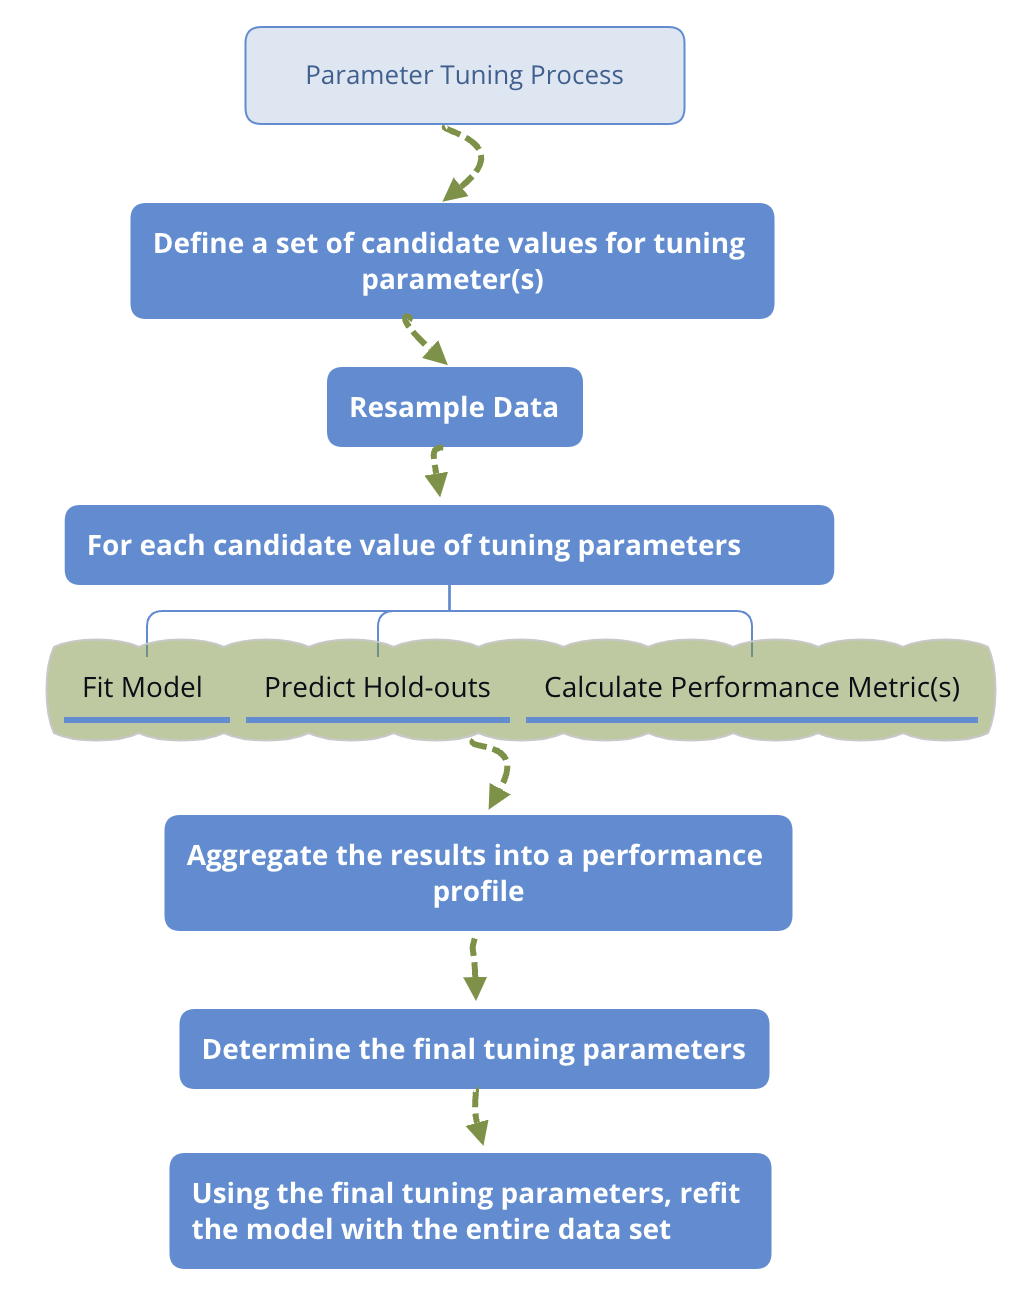
\includegraphics[width=0.80000\textwidth]{images/ParameterTuningProcess.png}
\caption{Parameter Tuning Process}
\end{figure}

The above is an outline of the general procedure to tune parameters. Now
let's focus on the critical part of the process: data splitting.
Ideally, we should evaluate model using samples that were not used to
build or fine-tune the model. So it provides an unbiased sense of model
effectiveness. When the sample size is large, it is a good practice to
set aside part of the samples to evaluate the final model. People use
``training'' data to indicate samples used to fit or fine-tune the model
and ``test'' or ``validation'' data set is used to validate performance.

The first decision to make for data splitting is to decide the
proportion of data in the test set. There are two factors to consider
here: (1) sample size; (2) computation intensity. If the sample size is
large enough which is the most common situation according to my
experience, you can try to use 20\%, 30\% and 40\% of the data as the
test set, and see which one works the best. If the model is
computationally intense, then you may consider starting from a smaller
sample of data to train the model hence will have a higher portion of
data in the test set. Depending on how it performs, you may need to
increase the training set. If the sample size is small, you can use
cross-validation or bootstrap which is the topic in the next section.

The next decision is to decide which samples are in the test set. There
is a desire to make the training and test sets as similar as possible. A
simple way is to split data by random sampling which, however, does not
control for any of the data attributes, such as the percentage of the
retained customer in the data. So it is possible that the distribution
of outcomes is substantially different between the training and test
sets. There are three main ways to split the data that account for the
similarity of resulted data sets. We will describe the three approaches
using the clothing company customer data as examples.

\begin{enumerate}
\def\labelenumi{(\arabic{enumi})}
\tightlist
\item
  Split data according to the outcome variable
\end{enumerate}

Assume the outcome variable is customer segment (column
\texttt{segment}) and we decide to use 80\% as training and 20\% test.
The goal is to make the proportions of the categories in the two sets as
similar as possible. The \texttt{createDataPartition()} function in
\texttt{caret} will return a balanced splitting based on assigned
variable.

\begin{Shaded}
\begin{Highlighting}[]
\CommentTok{# load data}
\NormalTok{sim.dat <-}\StringTok{ }\KeywordTok{read.csv}\NormalTok{(}\StringTok{"https://raw.githubusercontent.com/happyrabbit/DataScientistR/master/Data/SegData.csv"}\NormalTok{)}
\KeywordTok{library}\NormalTok{(caret)}
\CommentTok{# set random seed to make sure reproducibility}
\KeywordTok{set.seed}\NormalTok{(}\DecValTok{3456}\NormalTok{)}
\NormalTok{trainIndex <-}\StringTok{ }\KeywordTok{createDataPartition}\NormalTok{(sim.dat}\OperatorTok{$}\NormalTok{segment, }\DataTypeTok{p =} \FloatTok{0.8}\NormalTok{, }\DataTypeTok{list =} \OtherTok{FALSE}\NormalTok{, }
    \DataTypeTok{times =} \DecValTok{1}\NormalTok{)}
\KeywordTok{head}\NormalTok{(trainIndex)}
\end{Highlighting}
\end{Shaded}

\begin{verbatim}
##      Resample1
## [1,]         1
## [2,]         2
## [3,]         3
## [4,]         4
## [5,]         6
## [6,]         7
\end{verbatim}

The \texttt{list\ =\ FALSE} in the call to \texttt{createDataPartition}
is to return a data frame. The \texttt{times\ =\ 1} tells R how many
times you want to split the data. Here we only do it once, but you can
repeat the splitting multiple times. In that case, the function will
return multiple vectors indicating the rows to training/test. You can
set \texttt{times=2} and rerun the above code to see the result. Then
we can use the returned indicator vector \texttt{trainIndex} to get
training and test sets:

\begin{Shaded}
\begin{Highlighting}[]
\CommentTok{# get training set}
\NormalTok{datTrain <-}\StringTok{ }\NormalTok{sim.dat[trainIndex, ]}
\CommentTok{# get test set}
\NormalTok{datTest <-}\StringTok{ }\NormalTok{sim.dat[}\OperatorTok{-}\NormalTok{trainIndex, ]}
\end{Highlighting}
\end{Shaded}

According to the setting, there are 800 samples in the training set and
200 in test set. Let's check the distribution of the two sets:

\begin{Shaded}
\begin{Highlighting}[]
\KeywordTok{library}\NormalTok{(plyr)}
\KeywordTok{ddply}\NormalTok{(datTrain, }\StringTok{"segment"}\NormalTok{, summarise, }\DataTypeTok{count =} \KeywordTok{length}\NormalTok{(segment), }
    \DataTypeTok{percentage =} \KeywordTok{round}\NormalTok{(}\KeywordTok{length}\NormalTok{(segment)}\OperatorTok{/}\KeywordTok{nrow}\NormalTok{(datTrain), }\DecValTok{2}\NormalTok{))}
\end{Highlighting}
\end{Shaded}

\begin{verbatim}
##       segment count percentage
## 1 Conspicuous   160       0.20
## 2       Price   200       0.25
## 3     Quality   160       0.20
## 4       Style   280       0.35
\end{verbatim}

\begin{Shaded}
\begin{Highlighting}[]
\KeywordTok{ddply}\NormalTok{(datTest, }\StringTok{"segment"}\NormalTok{, summarise, }\DataTypeTok{count =} \KeywordTok{length}\NormalTok{(segment), }
    \DataTypeTok{percentage =} \KeywordTok{round}\NormalTok{(}\KeywordTok{length}\NormalTok{(segment)}\OperatorTok{/}\KeywordTok{nrow}\NormalTok{(datTest), }\DecValTok{2}\NormalTok{))}
\end{Highlighting}
\end{Shaded}

\begin{verbatim}
##       segment count percentage
## 1 Conspicuous    40       0.20
## 2       Price    50       0.25
## 3     Quality    40       0.20
## 4       Style    70       0.35
\end{verbatim}

The percentages are the same for these two sets. In practice, it is
possible that the distributions are not exactly identical but should be
close.

\begin{enumerate}
\def\labelenumi{(\arabic{enumi})}
\setcounter{enumi}{1}
\tightlist
\item
  Divide data according to predictors
\end{enumerate}

An alternative way is to split data based on the predictors. The goal is
to get a diverse subset from a dataset so that the sample is
representative. In other words, we need an algorithm to identify the
\(n\) most diverse samples from a dataset with size \(N\). However, the
task is generally infeasible for non-trivial values of \(n\) and \(N\)
\citep{willett}. And hence practicable approaches to dissimilarity-based
selection involve approximate methods that are sub-optimal. A major
class of algorithms split the data on \emph{maximum dissimilarity
sampling}. The process starts from:

\begin{itemize}
\tightlist
\item
  Initialize a single sample as starting test set
\item
  Calculate the dissimilarity between this initial sample and each
  remaining samples in the dataset
\item
  Add the most dissimilar unallocated sample to the test set
\end{itemize}

To move forward, we need to define the dissimilarity between groups.
Each definition results in a different version of the algorithm and
hence a different subset. It is the same problem as in hierarchical
clustering where you need to define a way to measure the distance
between clusters. The possible approaches are to use minimum, maximum,
sum of all distances, the average of all distances, etc. Unfortunately,
there is not a single best choice, and you may have to try multiple
methods and check the resulted sample sets. R users can implement the
algorithm using \texttt{maxDissim()} function from \texttt{caret}
package. The \texttt{obj} argument is to set the definition of
dissimilarity. Refer to the help documentation for more details
(\texttt{?maxDissim}).

Let's use two variables (\texttt{age} and \texttt{income}) from the
customer data as an example to illustrate how it works in R and compare
maximum dissimilarity sampling with random sampling.

\begin{Shaded}
\begin{Highlighting}[]
\KeywordTok{library}\NormalTok{(lattice)}
\CommentTok{# select variables}
\NormalTok{testing <-}\StringTok{ }\KeywordTok{subset}\NormalTok{(sim.dat, }\DataTypeTok{select =} \KeywordTok{c}\NormalTok{(}\StringTok{"age"}\NormalTok{, }\StringTok{"income"}\NormalTok{))}
\end{Highlighting}
\end{Shaded}

Random select 5 samples as initial subset (\texttt{start}) , the rest
will be in \texttt{samplePool}:

\begin{Shaded}
\begin{Highlighting}[]
\KeywordTok{set.seed}\NormalTok{(}\DecValTok{5}\NormalTok{)}
\CommentTok{# select 5 random samples}
\NormalTok{startSet <-}\StringTok{ }\KeywordTok{sample}\NormalTok{(}\DecValTok{1}\OperatorTok{:}\KeywordTok{dim}\NormalTok{(testing)[}\DecValTok{1}\NormalTok{], }\DecValTok{5}\NormalTok{)}
\NormalTok{start <-}\StringTok{ }\NormalTok{testing[startSet, ]}
\CommentTok{# save the rest in data frame 'samplePool'}
\NormalTok{samplePool <-}\StringTok{ }\NormalTok{testing[}\OperatorTok{-}\NormalTok{startSet, ]}
\end{Highlighting}
\end{Shaded}

Use \texttt{maxDissim()} to select another 5 samples from
\texttt{samplePool} that are as different as possible with the initical
set \texttt{start}:

\begin{Shaded}
\begin{Highlighting}[]
\NormalTok{selectId <-}\StringTok{ }\KeywordTok{maxDissim}\NormalTok{(start, samplePool, }\DataTypeTok{obj =}\NormalTok{ minDiss, }\DataTypeTok{n =} \DecValTok{5}\NormalTok{)}
\NormalTok{minDissSet <-}\StringTok{ }\NormalTok{samplePool[selectId, ]}
\end{Highlighting}
\end{Shaded}

The \texttt{obj\ =\ minDiss} in the above code tells R to use minimum
dissimilarity to define the distance between groups. Next, random select
5 samples from \texttt{samplePool} in data frame \texttt{RandomSet}:

\begin{Shaded}
\begin{Highlighting}[]
\NormalTok{selectId <-}\StringTok{ }\KeywordTok{sample}\NormalTok{(}\DecValTok{1}\OperatorTok{:}\KeywordTok{dim}\NormalTok{(samplePool)[}\DecValTok{1}\NormalTok{], }\DecValTok{5}\NormalTok{)}
\NormalTok{RandomSet <-}\StringTok{ }\NormalTok{samplePool[selectId, ]}
\end{Highlighting}
\end{Shaded}

Plot the resulted set to compare different sampling methods:

\begin{Shaded}
\begin{Highlighting}[]
\NormalTok{start}\OperatorTok{$}\NormalTok{group <-}\StringTok{ }\KeywordTok{rep}\NormalTok{(}\StringTok{"Initial Set"}\NormalTok{, }\KeywordTok{nrow}\NormalTok{(start))}
\NormalTok{minDissSet}\OperatorTok{$}\NormalTok{group <-}\StringTok{ }\KeywordTok{rep}\NormalTok{(}\StringTok{"Maximum Dissimilarity Sampling"}\NormalTok{, }\KeywordTok{nrow}\NormalTok{(minDissSet))}
\NormalTok{RandomSet}\OperatorTok{$}\NormalTok{group <-}\StringTok{ }\KeywordTok{rep}\NormalTok{(}\StringTok{"Random Sampling"}\NormalTok{, }\KeywordTok{nrow}\NormalTok{(RandomSet))}
\KeywordTok{xyplot}\NormalTok{(age }\OperatorTok{~}\StringTok{ }\NormalTok{income, }\DataTypeTok{data =} \KeywordTok{rbind}\NormalTok{(start, minDissSet, RandomSet), }\DataTypeTok{grid =} \OtherTok{TRUE}\NormalTok{, }
    \DataTypeTok{group =}\NormalTok{ group, }\DataTypeTok{auto.key =} \OtherTok{TRUE}\NormalTok{)}
\end{Highlighting}
\end{Shaded}

\begin{figure}

{\centering 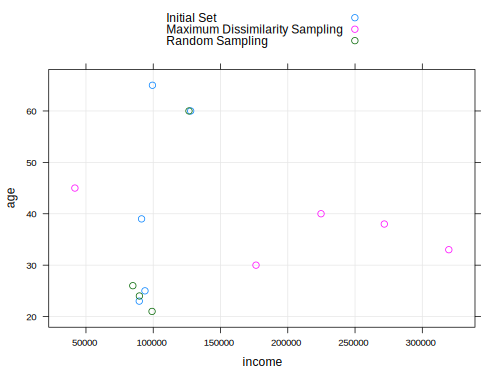
\includegraphics[width=0.8\linewidth]{IDS_files/figure-latex/maxdis-1} 

}

\caption{Compare Maximum Dissimilarity Sampling with  Random Sampling}\label{fig:maxdis}
\end{figure}

The points from maximum dissimilarity sampling are far away from the
initial samples ( Fig. \ref{fig:maxdis}, while the random samples are
much closer to the initial ones. Why do we need a diverse subset?
Because we hope the test set to be representative. If all test set
samples are from respondents younger than 30, model performance on the
test set has a high risk to fail to tell you how the model will perform
on more general population.

\begin{itemize}
\tightlist
\item
  Divide data according to time
\end{itemize}

For time series data, random sampling is usually not the best way. There
is an approach to divide data according to time-series. Since time
series is beyond the scope of this book, there is not much discussion
here. For more detail of this method, see \citep{Hyndman}. We will use a
simulated first-order autoregressive model {[}AR (1){]} time-series data
with 100 observations to show how to implement using the function
\texttt{createTimeSlices\ ()} in the \texttt{caret} package.

\begin{Shaded}
\begin{Highlighting}[]
\CommentTok{# simulte AR(1) time series samples}
\NormalTok{timedata =}\StringTok{ }\KeywordTok{arima.sim}\NormalTok{(}\KeywordTok{list}\NormalTok{(}\DataTypeTok{order=}\KeywordTok{c}\NormalTok{(}\DecValTok{1}\NormalTok{,}\DecValTok{0}\NormalTok{,}\DecValTok{0}\NormalTok{), }\DataTypeTok{ar=}\OperatorTok{-}\NormalTok{.}\DecValTok{9}\NormalTok{), }\DataTypeTok{n=}\DecValTok{100}\NormalTok{)}
\CommentTok{# plot time series}
\KeywordTok{plot}\NormalTok{(timedata, }\DataTypeTok{main=}\NormalTok{(}\KeywordTok{expression}\NormalTok{(}\KeywordTok{AR}\NormalTok{(}\DecValTok{1}\NormalTok{)}\OperatorTok{~}\ErrorTok{~~}\NormalTok{phi}\OperatorTok{==-}\NormalTok{.}\DecValTok{9}\NormalTok{)))     }
\end{Highlighting}
\end{Shaded}

\begin{figure}

{\centering 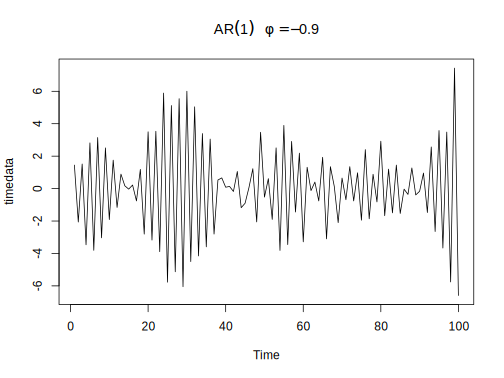
\includegraphics[width=0.8\linewidth]{IDS_files/figure-latex/times-1} 

}

\caption{Divide data according to time}\label{fig:times}
\end{figure}

Fig. \ref{fig:times} shows 100 simulated time series observation. The
goal is to make sure both training and test set to cover the whole
period.

\begin{Shaded}
\begin{Highlighting}[]
\NormalTok{timeSlices <-}\StringTok{ }\KeywordTok{createTimeSlices}\NormalTok{(}\DecValTok{1}\OperatorTok{:}\KeywordTok{length}\NormalTok{(timedata), }
                   \DataTypeTok{initialWindow =} \DecValTok{36}\NormalTok{, }\DataTypeTok{horizon =} \DecValTok{12}\NormalTok{, }\DataTypeTok{fixedWindow =}\NormalTok{ T)}
\KeywordTok{str}\NormalTok{(timeSlices,}\DataTypeTok{max.level =} \DecValTok{1}\NormalTok{)}
\end{Highlighting}
\end{Shaded}

\begin{verbatim}
## List of 2
##  $ train:List of 53
##  $ test :List of 53
\end{verbatim}

There are three arguments in the above \texttt{createTimeSlices()}.

\begin{itemize}
\tightlist
\item
  \texttt{initialWindow}: The initial number of consecutive values in
  each training set sample
\item
  \texttt{horizon}: the number of consecutive values in test set sample
\item
  \texttt{fixedWindow}: if FALSE, all training samples start at 1
\end{itemize}

The function returns two lists, one for the training set, the other for
the test set. Let's look at the first training sample:

\begin{Shaded}
\begin{Highlighting}[]
\CommentTok{# get result for the 1st training set}
\NormalTok{trainSlices <-}\StringTok{ }\NormalTok{timeSlices[[}\DecValTok{1}\NormalTok{]]}
\CommentTok{# get result for the 1st test set}
\NormalTok{testSlices <-}\StringTok{ }\NormalTok{timeSlices[[}\DecValTok{2}\NormalTok{]]}
\CommentTok{# check the index for the 1st training and test set}
\NormalTok{trainSlices[[}\DecValTok{1}\NormalTok{]]}
\end{Highlighting}
\end{Shaded}

\begin{verbatim}
##  [1]  1  2  3  4  5  6  7  8  9 10 11 12 13 14 15 16 17
## [18] 18 19 20 21 22 23 24 25 26 27 28 29 30 31 32 33 34
## [35] 35 36
\end{verbatim}

\begin{Shaded}
\begin{Highlighting}[]
\NormalTok{testSlices[[}\DecValTok{1}\NormalTok{]]}
\end{Highlighting}
\end{Shaded}

\begin{verbatim}
##  [1] 37 38 39 40 41 42 43 44 45 46 47 48
\end{verbatim}

The first training set is consist of sample 1-36 in the dataset
(\texttt{initialWindow\ =\ 36}). Then sample 37-48 are in the first test
set ( \texttt{horizon\ =\ 12}). Type \texttt{head(trainSlices)} or
\texttt{head(testSlices)} to check the later samples. If you are not
clear about the argument \texttt{fixedWindow}, try to change the setting
to be \texttt{F} and check the change in \texttt{trainSlices} and
\texttt{testSlices}.

Understand and implement data splitting is not difficult. But there are
two things to note:

\begin{enumerate}
\def\labelenumi{\arabic{enumi}.}
\tightlist
\item
  The randomness in the splitting process will lead to uncertainty in
  performance measurement.
\item
  When the dataset is small, it can be too expensive to leave out test
  set. In this situation, if collecting more data is just not possible,
  the best shot is to use leave-one-out cross-validation which is in the
  next section.
\end{enumerate}

\subsection{Resampling}\label{resampling}

You can consider resampling as repeated splitting. The basic idea is:
use part of the data to fit model and then use the rest of data to
calculate model performance. Repeat the process multiple times and
aggregate the results. The differences in resampling techniques usually
center around the ways to choose subsamples. There are two main reasons
that we may need resampling:

\begin{enumerate}
\def\labelenumi{\arabic{enumi}.}
\item
  Estimate tuning parameters through resampling. Some examples of models
  with such parameters are Support Vector Machine (SVM), models
  including the penalty (LASSO) and random forest.
\item
  For models without tuning parameter, such as ordinary linear
  regression and partial least square regression, the model fitting
  doesn't require resampling. But you can study the model stability
  through resampling.
\end{enumerate}

We will introduce three most common resampling techniques: k-fold
cross-validation, repeated training/test splitting, and bootstrap.

\subsubsection{k-fold cross-validation}\label{k-fold-cross-validation}

k-fold cross-validation is to partition the original sample into \(k\)
equal size subsamples (folds). Use one of the \(k\) folds to validate
the model and the rest \(k-1\) to train model. Then repeat the process
\(k\) times with each of the \(k\) folds as the test set. Aggregate the
results into a performance profile.

Denote by \(\hat{f}^{-\kappa}(X)\) the fitted function, computed with
the \(\kappa^{th}\) fold removed and \(x_i^\kappa\) the predictors for
samples in left-out fold. The process of k-fold cross-validation is as
follows:

\begin{quote}
\begin{enumerate}
\def\labelenumi{\arabic{enumi}.}
\tightlist
\item
  Partition the original sample into \(k\) equal size folds
\item
  for \(\kappa=1…k\)
\end{enumerate}

\begin{itemize}
\tightlist
\item
  Use data other than fold \(\kappa\) to train the model
  \(\hat{f}^{-\kappa}(X)\)
\item
  Apply \(\hat{f}^{-\kappa}(X)\) to predict fold \(\kappa\) to get
  \(\hat{f}^{-\kappa}(x_i^\kappa)\)
\end{itemize}

\begin{enumerate}
\def\labelenumi{\arabic{enumi}.}
\setcounter{enumi}{2}
\tightlist
\item
  Aggregate the results
  \[\hat{Error} = \frac{1}{N}\Sigma_{\kappa=1}^k\Sigma_{x_i^{\kappa}}L(y_i^{\kappa},\hat{f}^{-\kappa}(x_i^\kappa))\]
\end{enumerate}
\end{quote}

It is a standard way to find the value of tuning parameter that gives
you the best performance. It is also a way to study the variability of
model performance.

The following figure represents a 5-fold cross-validation example.

\begin{figure}
\centering
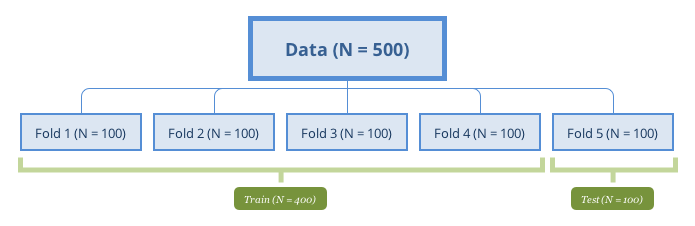
\includegraphics{images/cv5fold.png}
\caption{5-fold cross-validation}
\end{figure}

A special case of k-fold cross-validation is Leave One Out Cross
Validation (LOOCV) where \(k=1\). When sample size is small, it is
desired to use as many data to train the model. Most of the functions
have default setting \(k=10\). The choice is usually 5-10 in practice,
but there is no standard rule. The more folds to use, the more samples
are used to fit model, and then the performance estimate is closer to
the theoretical performance. Meanwhile, the variance of the performance
is larger since the samples to fit model in different iterations are
more similar. However, LOOCV has high computational cost since the
number of interactions is the same as the sample size and each model fit
uses a subset that is nearly the same size of the training set. On the
other hand, when k is small (such as 2 or 3), the computation is more
efficient, but the bias will increase. When the sample size is large,
the impact of \(k\) becomes marginal.

Chapter 7 of \citep{Hastie2008} presents a more in-depth and more
detailed discussion about the bias-variance trade-off in k-fold
cross-validation.

You can implement k-fold cross-validation using \texttt{createFolds()}
in \texttt{caret}:

\begin{Shaded}
\begin{Highlighting}[]
\KeywordTok{library}\NormalTok{(caret)}
\NormalTok{class<-sim.dat}\OperatorTok{$}\NormalTok{segment}
\CommentTok{# creat k-folds}
\KeywordTok{set.seed}\NormalTok{(}\DecValTok{1}\NormalTok{)}
\NormalTok{cv<-}\KeywordTok{createFolds}\NormalTok{(class,}\DataTypeTok{k=}\DecValTok{10}\NormalTok{,}\DataTypeTok{returnTrain=}\NormalTok{T)}
\KeywordTok{str}\NormalTok{(cv)}
\end{Highlighting}
\end{Shaded}

\begin{verbatim}
## List of 10
##  $ Fold01: int [1:900] 1 2 3 4 5 6 7 8 9 10 ...
##  $ Fold02: int [1:900] 1 2 3 4 5 6 7 9 10 11 ...
##  $ Fold03: int [1:900] 1 2 3 4 5 6 7 8 10 11 ...
##  $ Fold04: int [1:900] 1 2 3 4 5 6 7 8 9 11 ...
##  $ Fold05: int [1:900] 1 3 4 6 7 8 9 10 11 12 ...
##  $ Fold06: int [1:900] 1 2 3 4 5 6 7 8 9 10 ...
##  $ Fold07: int [1:900] 2 3 4 5 6 7 8 9 10 11 ...
##  $ Fold08: int [1:900] 1 2 3 4 5 8 9 10 11 12 ...
##  $ Fold09: int [1:900] 1 2 4 5 6 7 8 9 10 11 ...
##  $ Fold10: int [1:900] 1 2 3 5 6 7 8 9 10 11 ...
\end{verbatim}

The above code creates ten folds (\texttt{k=10}) according to the
customer segments (we set \texttt{class} to be the categorical variable
\texttt{segment}). The function returns a list of 10 with the index of
rows in training set.

\subsubsection{Repeated Training/Test
Splits}\label{repeated-trainingtest-splits}

In fact, this method is nothing but repeating the training/test set
division on the original data. Fit the model with the training set, and
evaluate the model with the test set. Unlike k-fold cross-validation,
the test set generated by this procedure may have duplicate samples. A
sample usually shows up in more than one test sets. There is no standard
rule for split ratio and number of repetitions. The most common choice
in practice is to use 75\% to 80\% of the total sample for training. The
remaining samples are for validation. The more sample in the training
set, the less biased the model performance estimate is. Increasing the
repetitions can reduce the uncertainty in the performance estimates. Of
course, it is at the cost of computational time when the model is
complex. The number of repetitions is also related to the sample size of
the test set. If the size is small, the performance estimate is more
volatile. In this case, the number of repetitions needs to be higher to
deal with the uncertainty of the evaluation results.

We can use the same function (\texttt{createDataPartition\ ()}) as
before. If you look back, you will see \texttt{times\ =\ 1}. The only
thing to change is to set it to the number of repetitions.

\begin{Shaded}
\begin{Highlighting}[]
\NormalTok{trainIndex <-}\StringTok{ }\KeywordTok{createDataPartition}\NormalTok{(sim.dat}\OperatorTok{$}\NormalTok{segment, }\DataTypeTok{p =}\NormalTok{ .}\DecValTok{8}\NormalTok{, }\DataTypeTok{list =} \OtherTok{FALSE}\NormalTok{, }\DataTypeTok{times =} \DecValTok{5}\NormalTok{)}
\NormalTok{dplyr}\OperatorTok{::}\KeywordTok{glimpse}\NormalTok{(trainIndex)}
\end{Highlighting}
\end{Shaded}

\begin{verbatim}
##  int [1:800, 1:5] 1 3 4 5 6 7 8 9 10 11 ...
##  - attr(*, "dimnames")=List of 2
##   ..$ : NULL
##   ..$ : chr [1:5] "Resample1" "Resample2" "Resample3" "Resample4" ...
\end{verbatim}

Once know how to split the data, the repetition comes naturally.

\subsubsection{Bootstrap Methods}\label{bootstrap-methods}

Bootstrap is a powerful statistical tool (a little magic too). It can be
used to analyze the uncertainty of parameter estimates
\citep{bootstrap1986} quantitatively. For example, estimate the standard
deviation of linear regression coefficients. The power of this method is
that the concept is so simple that it can be easily applied to any model
as long as the computation allows. However, you can hardly obtain the
standard deviation for some models by using the traditional statistical
inference.

Since it is with replacement, a sample can be selected multiple times,
and the bootstrap sample size is the same as the original data. So for
every bootstrap set, there are some left-out samples, which is also
called ``out-of-bag samples.'' The out-of-bag sample is used to evaluate
the model. Efron points out that under normal circumstances
\citep{efron1983}, bootstrap estimates the error rate of the model with
more certainty.The probability of an observation \(i\) in bootstrap
sample B is:

\(\begin{array}{ccc} Pr{i\in B} & = & 1-\left(1-\frac{1}{N}\right)^{N}\\  & \approx & 1-e^{-1}\\  & = & 0.632 \end{array}\)

On average, 63.2\% of the observations appeared at least once in a
bootstrap sample, so the estimation bias is similar to 2-fold
cross-validation. As mentioned earlier, the smaller the number of folds,
the larger the bias. Increasing the sample size will ease the problem.
In general, bootstrap has larger bias and smaller uncertainty than
cross-validation. Efron came up the following ``.632 estimator'' to
alleviate this bias:

\[(0.632 × original\ bootstrap\ estimate) + (0.368 × apparent\ error\ rate)\]

The apparent error rate is the error rate when the data is used twice,
both to fit the model and to check its accuracy and it is apparently
over-optimistic. The modified bootstrap estimate reduces the bias but
can be unstable with small samples size. This estimate can also be
unduly optimistic when the model severely over-fits since the apparent
error rate will be close to zero. Efron and Tibshirani \citep{b632plus}
discuss another technique, called the ``632+ method,'' for adjusting the
bootstrap estimates.

\chapter{Measuring Performance}\label{measuring-performance}

In order to compare different models, we need a way to measure model
performance. There are different metrics to use. Sometimes, it is better
to look at models through multiple lens. In this chapter, we will
introduce some of the most common measurement metrics.

\section{Regression Model
Performance}\label{regression-model-performance}

\section{Classification Model
Performance}\label{classification-model-performance}

\chapter{Feature Engineering}\label{feature-engineering}

\section{Feature Construction}\label{feature-construction}

\section{Feature Extraction}\label{feature-extraction}

\section{Feature Selection}\label{feature-selection}

\subsection{Filter Method}\label{filter-method}

\subsection{Wrapper Method}\label{wrapper-method}

\chapter{Regression Models}\label{regression-models}

\section{Ordinary Least Squares}\label{ordinary-least-squares}

\section{Multivariate Adaptive Regression
Splines}\label{multivariate-adaptive-regression-splines}

\section{Generalized Linear Model}\label{generalized-linear-model}

\section{PCR and PLS}\label{pcr-and-pls}

\chapter{Regularization Methods}\label{regularization-methods}

\section{Ridge Regression}\label{ridge-regression}

\section{LASSO}\label{lasso}

\section{Elastic Net}\label{elastic-net}

\section{LASSO Generalized Linear
Model}\label{lasso-generalized-linear-model}

\chapter{Tree-Based Methods}\label{tree-based-methods}

The tree-based models can be used for regression and classification.
They are conceptually simple yet powerful. This type of model is often
referred to as Classification And Regression Trees (CART). They are
popular tools for many reasons:

\begin{enumerate}
\def\labelenumi{\arabic{enumi}.}
\tightlist
\item
  Do not require user to specify the form of the relationship between
  predictors and response
\item
  Do not require (or if they do, very limited) data preprocessing and
  can handle different types of predictors (sparse, skewed, continuous,
  categorical, etc.)
\item
  Robust to co-linearity
\item
  Can handle missing data
\item
  Many pre-built packages make implementation as easy as a button push
\end{enumerate}

CART can refer to the tree model in general, but most of the time, it
represents the algorithm initially proposed by Breiman
\citep{Breiman1984}. After Breiman, there are many new algorithms, such
as ID3, C4.5, and C5.0. C5.0 is an improved version of C4.5, but since
C5.0 is not open source, the C4.5 algorithm is more popular. C4.5 was a
major competitor of CART. But now, all those seem outdated. The most
popular tree models are Random Forest (RF) and Gradient Boosting Machine
(GBM). Despite being out of favor in application, it is important to
understand the mechanism of the basic tree algorithm. Because the later
models are based on the same foundation.

The original CART algorithm targets binary classification, and the later
algorithms can handle multi-category classification. A single tree is
easy to explain but has poor accuracy. More complicated tree models,
such as RF and GBM, can provide much better prediction at the cost of
explainability. As the model becoming more complicated, it is more like
a black-box which makes it very difficult to explain the relationship
among predictors. There is always a trade-off between explainability and
predictability.

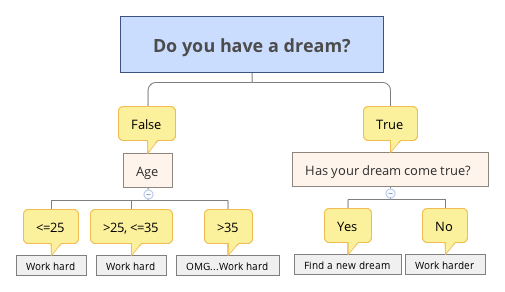
\includegraphics{../linhui.org/book/Figure/treeEN.png}

The reason why it is called ``tree'' is of course because the structure
has similarities. But the direction of the decision tree is opposite to
the real tree, the root is on the top, and the leaf is on the bottom.
From the root node, a decision tree divides to different branches and
generates more nodes. The new nodes are child nodes, and the previous
node is the parent node. At each child node, the algorithm will decide
whether to continue dividing. If it stops, the node is called a leaf
node. If it continues, then the node becomes the new parent node and
splits to produce the next layer of child nodes. At each non-leaf node,
the algorithm needs to decide split into branches. The leaf node
contains the final ``decision,'' final class the sample belongs to or
the sample's value has. Here are the important definitions in the tree
model:

\begin{itemize}
\tightlist
\item
  \textbf{Classification tree}: the outcome is discrete
\item
  \textbf{Regression tree}: the outcome is continuous (e.g.~the price of
  a house, or a patient's length of stay in a hospital)
\item
  \textbf{Non-leaf node (or split node)}: the algorithm needs to decide
  a split at each non-leaf node (eg: \(age \leq 25\),
  \(25 < age \leq 35\), \(age > 35\))
\item
  \textbf{Root node}:the beginning node where the tree starts
\item
  \textbf{Leaf node (or Terminal node)}: the node stops splitting. It
  has the final decision of the model
\item
  \textbf{Degree of the node}: the number of subtrees of a node
\item
  \textbf{Degree of the tree}: the maximum degree of a node in the tree
\item
  \textbf{Pruning}: remove parts of the tree that do not provide power
  to classify instances
\item
  \textbf{Branch (or Subtree)}: the whole part under a non-leaf node
\item
  \textbf{Child}: the node directly after and connected to another node
\item
  \textbf{Parent}: the converse notion of a child
\end{itemize}

Single tree is easy to explain but has high variance and low accuracy,
and hence is very limited. Minor changes in the training data can lead
to large changes in the fitted tree. A series of rectangular decision
regions defined by a single tree is often too naive to represent the
relationship between the dependent variable and the predictors. To
overcome these shortcomings, researchers have proposed ensemble methods
which combine many trees. Ensemble tree models typically have much
better predictive performance than a single tree. We will introduce
those models in later sections.

\section{Splitting Criteria}\label{splitting-criteria}

The splitting criteria used by the regression tree and the
classification tree are different. Like the regression tree, the goal of
the classification tree is to divide the data into smaller, more
homogeneous groups. Homogeneity means that most of the samples at each
node are from one class. The original CART algorithm uses Gini impurity
as the splitting criterion; The later ID3, C4.5, and C5.0 use entropy.
We will look at three most common splitting criteria.

\textbf{Gini impurity}

Gini impurity\citep{Breiman1984} is a measure of non-homogeneity. It is
widely used in classification tree. For a two-class problem, the Gini
impurity for a given node is defined as:

\[p_{1}(1-p_{1})+p_{2}(1-p_{2})\]

where \(p_{1}\) and \(p_{2}\) are probabilities for the two classes
respectively. It is easy to see that when the sample set is pure, one of
the probability is 0 and the Gini score is the smallest. Conversely,
when \(p_{1}=p_{2}=0.5\), the Gini score is the largest, in which case
the purity of the node is the smallest. Let's look at an example.
Suppose we want to determine which students are computer science (CS)
majors. Here is the simple hypothetical classification tree result
obtained with the gender variable.

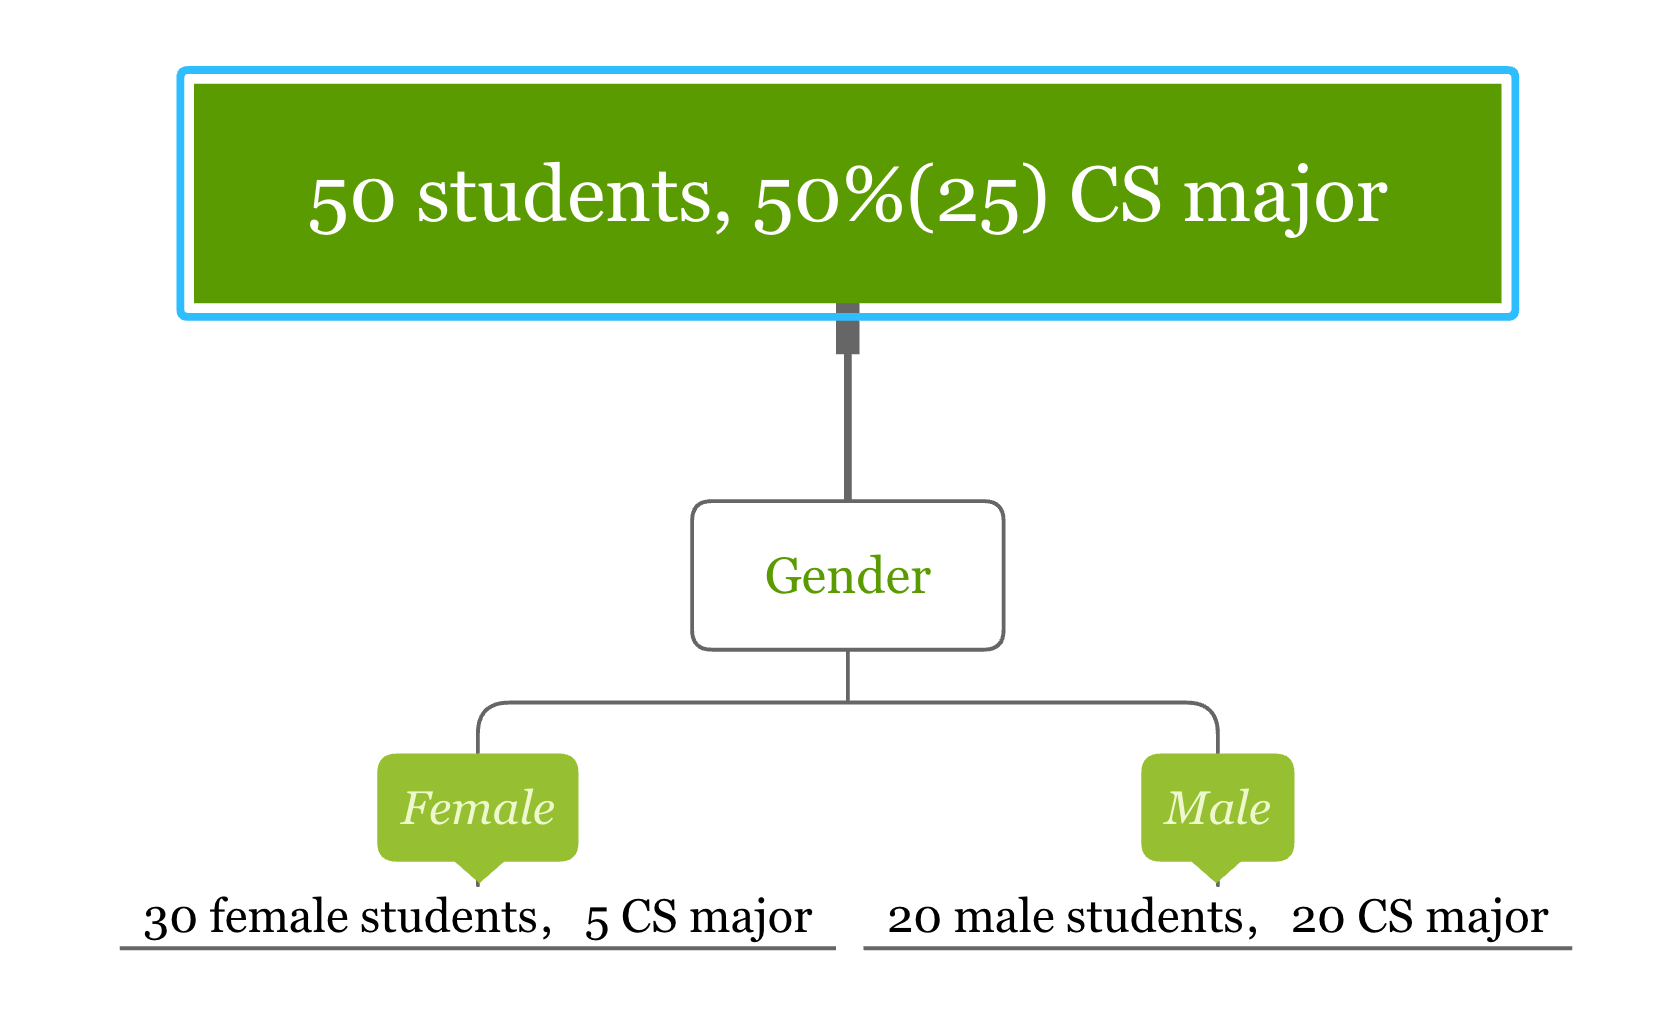
\includegraphics{../linhui.org/book/Figure/giniEN.PNG}

Let's calculate the Gini impurity for splitting node ``Gender'':

\begin{enumerate}
\def\labelenumi{\arabic{enumi}.}
\tightlist
\item
  Gini impurity for ``Female'' =
  \(\frac{1}{6}\times\frac{5}{6}+\frac{5}{6}\times\frac{1}{6}=\frac{5}{18}\)
\item
  Gini impurity for ``Male'' = \(0\times1+1\times 0=0\)
\end{enumerate}

The Gini impurity for the node ``Gender'' is the following weighted
average of the above two scores:

\[\frac{3}{5}\times\frac{5}{18}+\frac{2}{5}\times 0=\frac{1}{6}\]

The Gini impurity for the 50 samples in the parent node is
\(\frac{1}{2}\). It is easy to calculate the Gini impurity drop from
\(\frac{1}{2}\) to \(\frac{1}{6}\) after splitting. The split using
``gender'' causes a Gini impurity decrease of \(\frac{1}{3}\). The
algorithm will use different variables to split the data and choose the
one that causes the most substantial Gini impurity decrease.

\textbf{Information gain}

Looking at the samples in the following three nodes, which one is the
easiest to describe? It is obviously C. Because all the samples in C are
of the same type, so the description requires the least amount of
information. On the contrary, B needs more information, and A needs the
most information. In other words, C has the highest purity, B is the
second, and A has the lowest purity. We need less information to
describe nodes with lower purity.

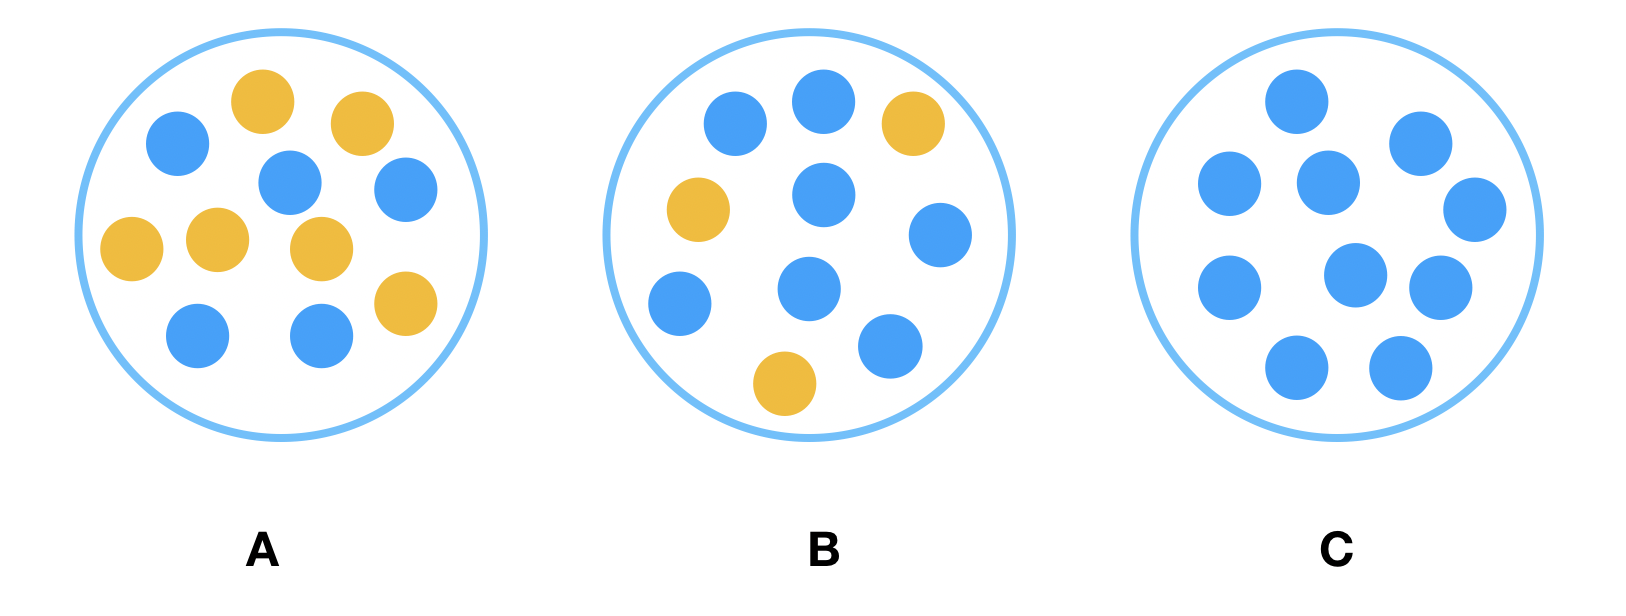
\includegraphics{../linhui.org/book/Figure/InfoGainEN.PNG}

A measure of the degree of disorder is entropy which is defined as:

\[Entropy=-plog_{2}p-(1-p)log_{2}(1-p)\]

where p is the percentage of one type of samples. If all the samples in
one node are of one type (such as C), the entropy is 0. If the
proportion of each type in a node is 50\%-50\%, the entropy is 1. We
can use entropy as splitting criteria. The goal is to decrease entropy
as the tree grows.

Similarly, the entropy of a splitting node is the weighted average of
the entropy of each child. In the above tree for the students, the
entropy of the root node with all 50 students is
\(-\frac{25}{50}log_{2}\frac{25}{50}-\frac{25}{50}log_{2}\frac{25}{50}=1\).
Here an entropy of 1 indicates that the purity of the node is the
lowest, that is, each type takes up half of the samples.

The entropy of the split using variable ``gender'' can be calculated in
three steps:

\begin{enumerate}
\def\labelenumi{\arabic{enumi}.}
\tightlist
\item
  Entropy for ``Female'' =
  \(-\frac{5}{30}log_{2}\frac{5}{30}-\frac{25}{30}log_{2}\frac{25}{30}=0.65\)
\item
  Entropy for ``Male'' = \(0\times1+1\times 0=0\)
\item
  Entropy for the node ``Gender'' is the weighted average of the above
  two entropy numbers:
  \(\frac{3}{5}\times 0.65+\frac{2}{5}\times 0=0.39\)
\end{enumerate}

So entropy decreases from 1 to 0.39 after the split.

\textbf{Sum of Square Error (SSE)}

The previous two metrics are for classification tree. The SSE is the
most widely used splitting metric for regression. Suppose you want to
divide the data set \(S\) into two groups of \(S_{1}\) and \(S_{2}\),
where the selection of \(S_{1}\) and \(S_{2}\) needs to minimize the sum
of squared errors:

\begin{equation}
SSE=\Sigma_{i\in S_{1}}(y_{i}-\bar{y}_{1})^{2}+\Sigma_{i\in S_{2}}(y_{i}-\bar{y}_{2})^{2}
\label{eq:treesse}
\end{equation}

In equation \eqref{eq:treesse}, \(\bar{y}_{1}\) and \(\bar{y}_{1}\) are
the average of the sample in \(S_{1}\) and \(S_{2}\). The way regression
tree grows is to automatically decide on the splitting variables and
split points that can maximize \textbf{SSE reduction}. Since this
process is essentially a recursive segmentation, this approach is also
called recursive partitioning.

Take a look at this simple regression tree for the height of 10
students:

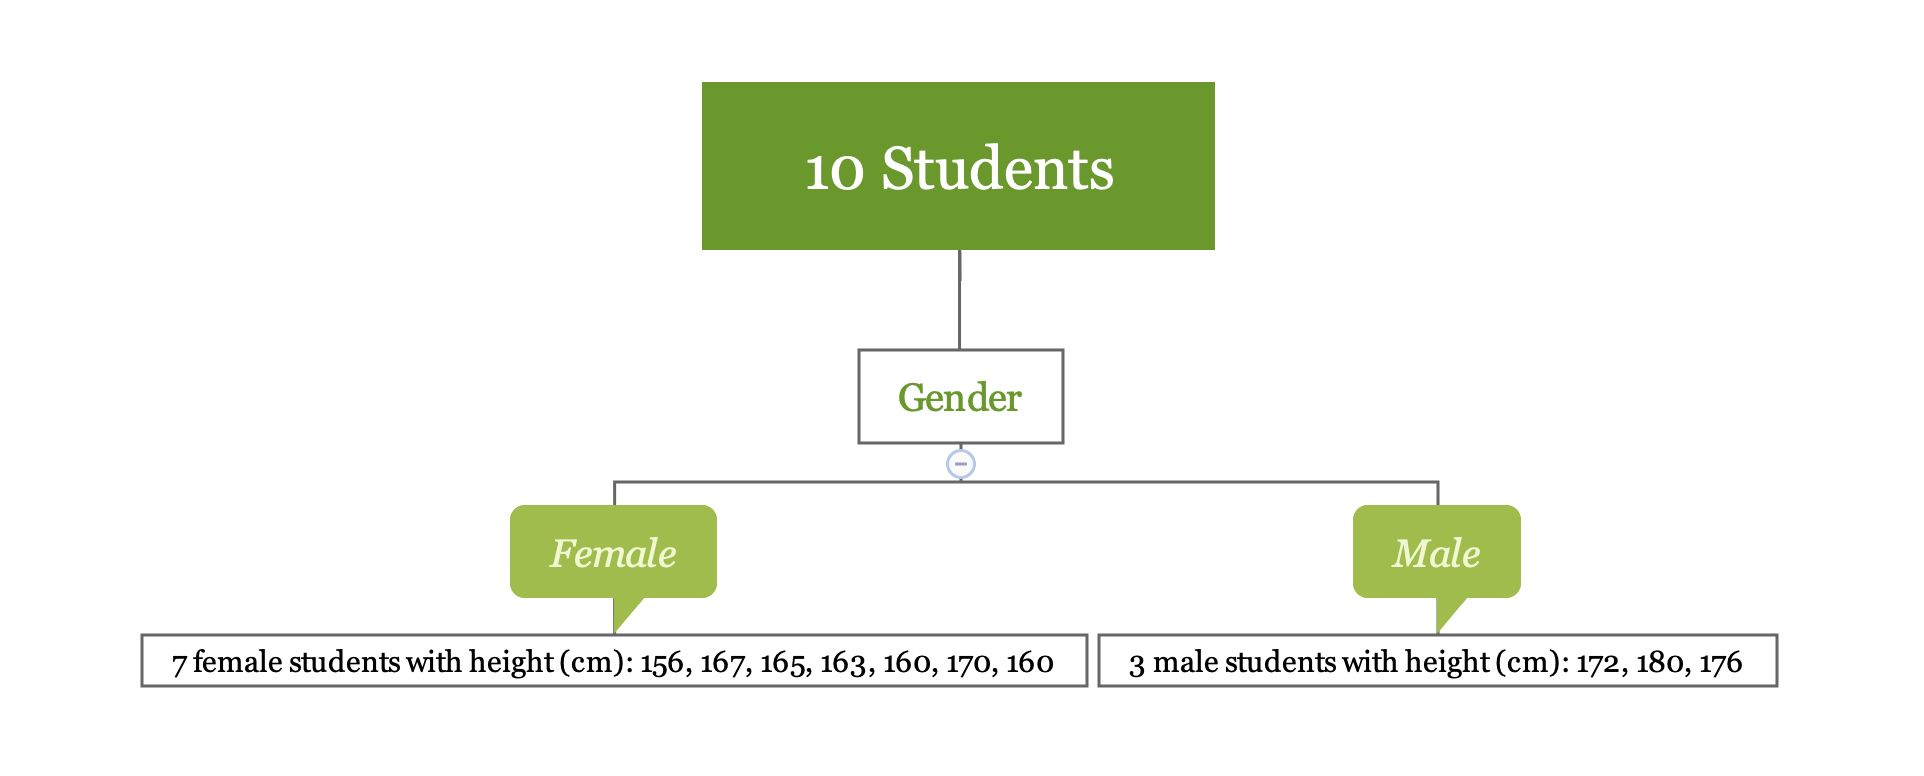
\includegraphics{images/varEN.png}

You can calculate the SSE using the following code:

\begin{enumerate}
\def\labelenumi{\arabic{enumi}.}
\tightlist
\item
  SSE for ``Female'' is 136
\item
  SSE for ``Male'' is 32
\item
  SSE for splitting node ``Gender'' is the sum of the above two numbers
  which is 168
\end{enumerate}

SSE for the 10 students in root node is 522.9. After the split, SSE
decreases from 522.9 to 168.

If there is another possible way of splitting, divide it by major, as
follows:

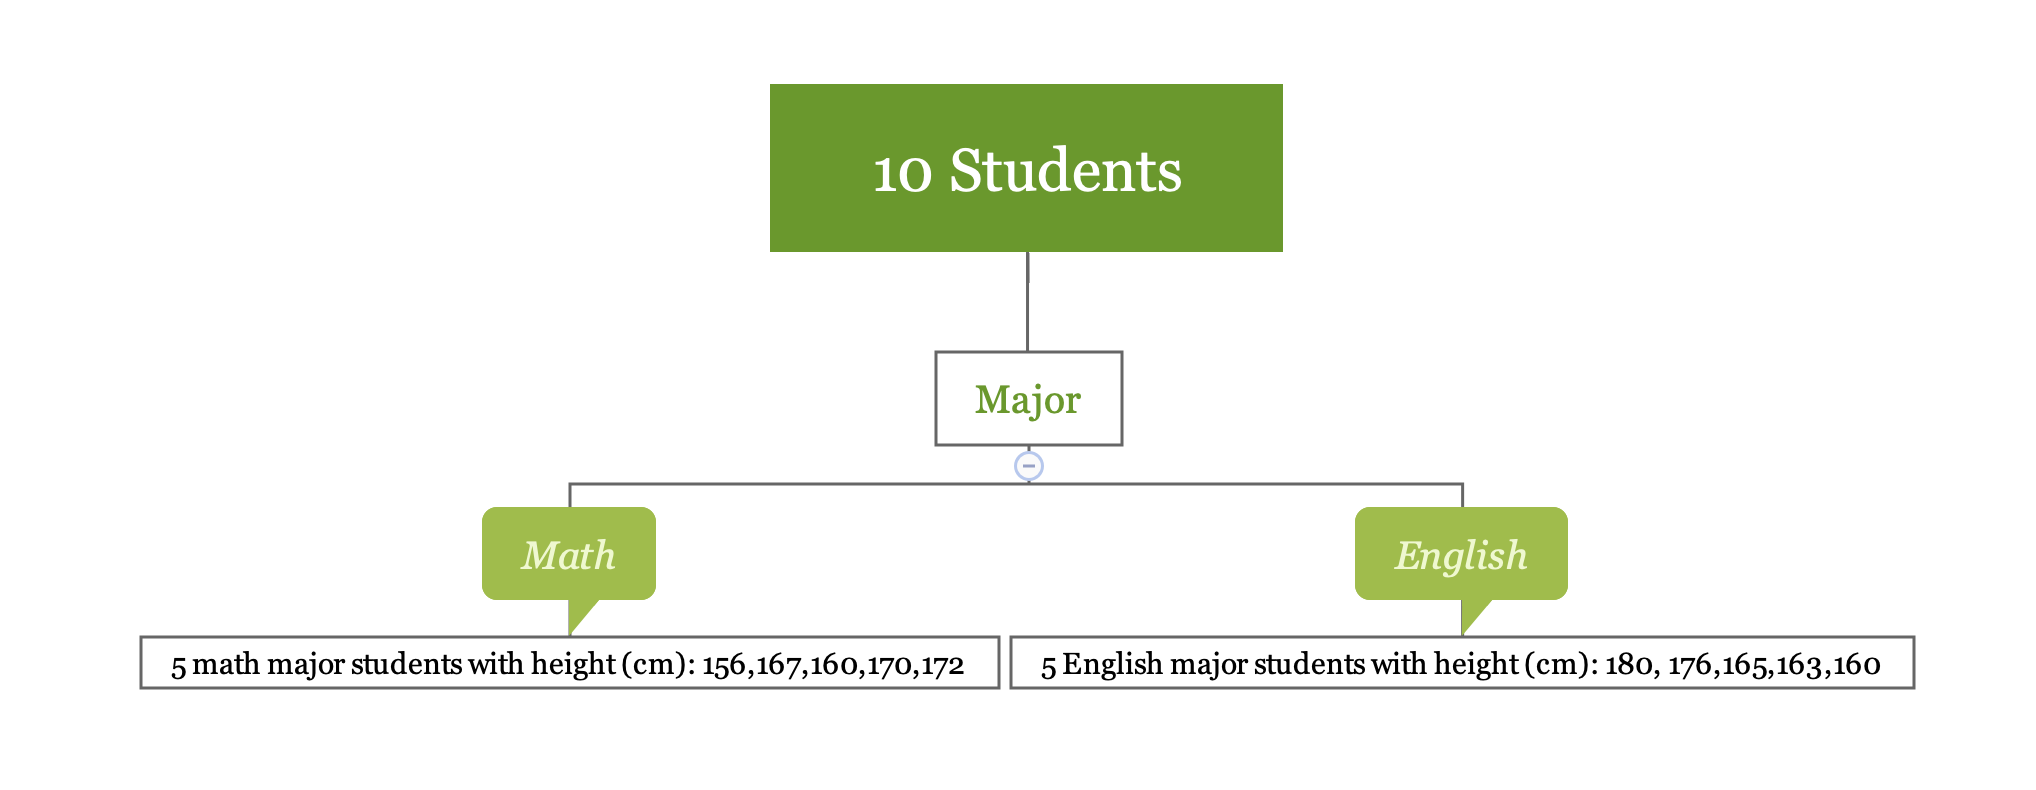
\includegraphics{images/varEN2.png}

In this situation:

\begin{enumerate}
\def\labelenumi{\arabic{enumi}.}
\tightlist
\item
  SSE for ``Math'' is 184
\item
  SSE for ``English'' is 302.8
\item
  SSE for splitting node ``Major'' is the sum of the above two numbers
  which is 486.8
\end{enumerate}

Splitting data using variable ``gender'' reduced SSE from 522.9 to 168;
using variable ``major'' reduced SSE from 522.9 to 486.8. Based on SSE
reduction, you should use gender to split the data.

The three splitting criteria mentioned above are the basis for building
a tree model.

\section{Tree Pruning}\label{tree-pruning}

Pruning is the process that reduces the size of decision trees. It
reduces the risk of overfitting by limiting the size of the tree or
removing sections of the tree that provide little power.

\textbf{Limit the size}

You can limit the tree size by setting some parameters.

\begin{itemize}
\item
  Minimum sample size at each node: Defining the minimum sample size at
  the node helps to prevent the leaf nodes having only one sample. The
  sample size can be a tuning parameter. If it is too large, the model
  tends to under-fit. If it is too small, the model tends to over-fit.
  In the case of severe class imbalance, the minimum sample size may
  need to be smaller because the number of samples in a particular class
  is small.
\item
  Maximum depth of the tree: If the tree grows too deep, the model tends
  to over-fit. It can be a tuning parameter.
\item
  Maximum number of terminal nodes: Limit on the terminal nodes works
  the same as the limit on the depth of the tree. They are proportional.
\item
  The number of variables considered for each split: the algorithm
  randomly selects variables used in finding the optimal split point at
  each level. In general, the square root of the number of all variables
  works best, which is also the default setting for many functions.
  However, people often treat it as a tuning parameter.
\end{itemize}

\section{Regression and Decision Tree
Basic}\label{regression-and-decision-tree-basic}

\section{Bagging Tree}\label{bagging-tree-1}

\section{Random Forest}\label{random-forest}

\section{Gradient Boosted Machine}\label{gradient-boosted-machine}

\chapter{Neural Network}\label{neural-network}

\section{Projection Pursuit
Regression}\label{projection-pursuit-regression}

Before moving onto neural networks, let us start with a broader
framework, Projection Pursuit Regression (PPR). It has a form of
\textbf{additive model} of the derived features rather than the inputs
themselves. Another widely used algorithm, AdaBoost, also fits an
additive model in a base learner.

Assume \(\mathbf{X^{T}}=(X_1,X_2,\dots,X_p)\) is a vector with \(p\)
variables. \(Y\) is the corresponding response variable.
\(\mathbf{\omega_{m}},m=1,2,\dots,M\) is parameter vector with \(p\)
elements.

\[f(\mathbf{X})=\sum_{m=1}^{M}g_{m}(\mathbf{\omega_{m}^{T}X})\]

The new feature \(\mathbf{V_{m}}=\mathbf{\omega_{m}^{T}X}\) is a linear
combination of input variables \(\mathbf{X}\). The additive model is
based on the new features. Here \(\mathbf{\omega_{m}}\) is a unit
vector, and the new feature \(\mathbf{v_m}\) is actually the projection
of \(\mathbf{X}\) on \(\mathbf{\omega_{m}}\). It projects the
p-dimensional independent variable space onto the new M-dimensional
feature space. This is similar to the principal component analysis
except that the principal component is orthogonal projection but it is
not necessarily orthogonal here.

I know it is very abstract. Let's look at some examples. Assume \(p=2\),
i.e.~there are two variables \(x_1\) and \(x_2\). If \(M=1\),
\(\mathbf{\omega^{T}}=(\frac{1}{2},\frac{\sqrt{3}}{2})\), then the
corresponding \(v=\frac{1}{2}x_{1}+\frac{\sqrt{3}}{2}x_{2}\). Let's try
different setings and compare the results:

\begin{enumerate}
\def\labelenumi{\arabic{enumi}.}
\item
  \(\mathbf{\omega^{T}}=(\frac{1}{2},\frac{\sqrt{3}}{2})\),
  \(v=\frac{1}{2}x_{1}+\frac{\sqrt{3}}{2}x_{2}\) ,
  \(g(v)=\frac{1}{1+e^{-v}}\)
\item
  \(\mathbf{\omega^{T}}=(1,0)\), \(v = x_1\),
  \(g(v)=(v+5)sin(\frac{1}{\frac{v}{3}+0.1})\)
\item
  \(\mathbf{\omega^{T}}=(0,1)\), \(v = x_2\), \(g(v)=e^{\frac{v^2}{5}}\)
\item
  \(\mathbf{\omega^{T}}=(1,0)\), \(v = x_1\),
  \(g(v)=(v+0.1)sin(\frac{1}{\frac{v}{3}+0.1})\)
\end{enumerate}

Here is how you can simulate the data and plot it using R:

\begin{Shaded}
\begin{Highlighting}[]
\CommentTok{# use plot3D package to generate 3D plot}
\KeywordTok{library}\NormalTok{(plot3D)}
\CommentTok{# get x1 and x2 note here x1 and x2 need to be matrix if you check the}
\CommentTok{# two objects, you will find: columns in x1 are identical rows in x2}
\CommentTok{# are identical mesh() is funciton from plot3D package you may need to}
\CommentTok{# think a little here}
\NormalTok{M <-}\StringTok{ }\KeywordTok{mesh}\NormalTok{(}\KeywordTok{seq}\NormalTok{(}\OperatorTok{-}\FloatTok{13.2}\NormalTok{, }\FloatTok{13.2}\NormalTok{, }\DataTypeTok{length.out =} \DecValTok{50}\NormalTok{), }\KeywordTok{seq}\NormalTok{(}\OperatorTok{-}\FloatTok{37.4}\NormalTok{, }\FloatTok{37.4}\NormalTok{, }\DataTypeTok{length.out =} \DecValTok{50}\NormalTok{))}
\NormalTok{x1 <-}\StringTok{ }\NormalTok{M}\OperatorTok{$}\NormalTok{x}
\NormalTok{x2 <-}\StringTok{ }\NormalTok{M}\OperatorTok{$}\NormalTok{y}
\NormalTok{## setting 1 map X using w to get v}
\NormalTok{v <-}\StringTok{ }\NormalTok{(}\DecValTok{1}\OperatorTok{/}\DecValTok{2}\NormalTok{) }\OperatorTok{*}\StringTok{ }\NormalTok{x1 }\OperatorTok{+}\StringTok{ }\NormalTok{(}\KeywordTok{sqrt}\NormalTok{(}\DecValTok{3}\NormalTok{)}\OperatorTok{/}\DecValTok{2}\NormalTok{) }\OperatorTok{*}\StringTok{ }\NormalTok{x2}
\CommentTok{# apply g() on v}
\NormalTok{g1 <-}\StringTok{ }\DecValTok{1}\OperatorTok{/}\NormalTok{(}\DecValTok{1} \OperatorTok{+}\StringTok{ }\KeywordTok{exp}\NormalTok{(}\OperatorTok{-}\NormalTok{v))}
\KeywordTok{par}\NormalTok{(}\DataTypeTok{mfrow =} \KeywordTok{c}\NormalTok{(}\DecValTok{2}\NormalTok{, }\DecValTok{2}\NormalTok{), }\DataTypeTok{mar =} \KeywordTok{c}\NormalTok{(}\DecValTok{0}\NormalTok{, }\DecValTok{0}\NormalTok{, }\DecValTok{1}\NormalTok{, }\DecValTok{0}\NormalTok{))}
\KeywordTok{surf3D}\NormalTok{(x1, x2, g1, }\DataTypeTok{colvar =}\NormalTok{ g1, }\DataTypeTok{border =} \StringTok{"black"}\NormalTok{, }\DataTypeTok{colkey =} \OtherTok{FALSE}\NormalTok{, }\DataTypeTok{box =} \OtherTok{FALSE}\NormalTok{, }
    \DataTypeTok{main =} \StringTok{"Setting 1"}\NormalTok{)}
\NormalTok{## setting 2}
\NormalTok{v <-}\StringTok{ }\NormalTok{x1}
\NormalTok{g2 <-}\StringTok{ }\NormalTok{(v }\OperatorTok{+}\StringTok{ }\DecValTok{5}\NormalTok{) }\OperatorTok{*}\StringTok{ }\KeywordTok{sin}\NormalTok{(}\DecValTok{1}\OperatorTok{/}\NormalTok{(v}\OperatorTok{/}\DecValTok{3} \OperatorTok{+}\StringTok{ }\FloatTok{0.1}\NormalTok{))}
\KeywordTok{surf3D}\NormalTok{(x1, x2, g2, }\DataTypeTok{colvar =}\NormalTok{ g2, }\DataTypeTok{border =} \StringTok{"black"}\NormalTok{, }\DataTypeTok{colkey =} \OtherTok{FALSE}\NormalTok{, }\DataTypeTok{box =} \OtherTok{FALSE}\NormalTok{, }
    \DataTypeTok{main =} \StringTok{"Setting 2"}\NormalTok{)}
\NormalTok{## setting 3}
\NormalTok{v <-}\StringTok{ }\NormalTok{x2}
\NormalTok{g3 <-}\StringTok{ }\KeywordTok{exp}\NormalTok{(v}\OperatorTok{^}\DecValTok{2}\OperatorTok{/}\DecValTok{5}\NormalTok{)}
\KeywordTok{surf3D}\NormalTok{(x1, x2, g3, }\DataTypeTok{colvar =}\NormalTok{ g3, }\DataTypeTok{border =} \StringTok{"black"}\NormalTok{, }\DataTypeTok{colkey =} \OtherTok{FALSE}\NormalTok{, }\DataTypeTok{box =} \OtherTok{FALSE}\NormalTok{, }
    \DataTypeTok{main =} \StringTok{"Setting 3"}\NormalTok{)}
\NormalTok{## setting 4}
\NormalTok{v <-}\StringTok{ }\NormalTok{x1}
\NormalTok{g4 <-}\StringTok{ }\NormalTok{(v }\OperatorTok{+}\StringTok{ }\FloatTok{0.1}\NormalTok{) }\OperatorTok{*}\StringTok{ }\KeywordTok{sin}\NormalTok{(}\DecValTok{1}\OperatorTok{/}\NormalTok{(v}\OperatorTok{/}\DecValTok{3} \OperatorTok{+}\StringTok{ }\FloatTok{0.1}\NormalTok{))}
\KeywordTok{surf3D}\NormalTok{(x1, x2, g4, }\DataTypeTok{colvar =}\NormalTok{ g4, }\DataTypeTok{border =} \StringTok{"black"}\NormalTok{, }\DataTypeTok{colkey =} \OtherTok{FALSE}\NormalTok{, }\DataTypeTok{box =} \OtherTok{FALSE}\NormalTok{, }
    \DataTypeTok{main =} \StringTok{"Setting 4"}\NormalTok{)}
\end{Highlighting}
\end{Shaded}

\includegraphics{IDS_files/figure-latex/nnet_simulate_data-1.pdf}

You can see that this framework is very flexible. In essence, it is to
do a non-linear transformation of the linear combination. You can use
this way to capture varies of relationships. For example,\(x_{1}x_{2}\)
can be written as \(\frac{(x_{1}+x_{2})^{2}-(x_{1}-x_{2})^{2}}{4}\),
where \(M=2\). All the higher order factors of \(x_1\) and \(x_2\) can
be represented similarly. If \(M\) is large enough, this framework can
approximate any continuous function on \(\mathbb{R}^{p}\). So the model
family covers a board area, but with a price. That is the
interpretability. Because the number of parameters increases with M and
the mode is nested.

PPR in 1981 was a new idea then which lead to the debut of the neural
network model. The basic technical idea behind deep learning has been
around for decades. However, why did they take off in recent years? Here
are some main drivers behind the rise.

First, thanks to the digitalization where lots of human activities are
now in the digital realm and captured as data. So in the last 10 year,
for many problems, we went from having a relatively small amount of data
to accumulating a large amount of data. The traditional learning
algorithms, like Logistic Regression, Support Vector Machine, Random
Forest cannot effectively take advantage of such big data. Second, the
increasing computation power enables us to train a large neural network
either on a CPU or GPU using big data. The scale of data and computation
ability lead to much progress, but tremendous algorithmic innovation is
also an important driver. Many of the innovations are about speeding up
the optimization of neural network. One of the examples is to use ReLU
as intermediate layer activation function instead of the previous
sigmoid function. The change has made the optimization process much
faster because the previous sigmoid function suffers from vanishing
gradient. We will talk more about that in the following sections. Here
we just want to show an example of the impact of algorithmic innovation.

\section{Standard Neural Network}\label{standard-neural-network}

\subsection{Logistic Regression as Neural
Network}\label{logistic_reg_as_neural_network}

Let's look at logistic regression from the lens of neural network. For a
binary classification problem, for example spam classifier, given \(m\)
samples
\(\{(x^{(1)}, y^{(1)}),(x^{(2)}, y^{(2)}),...,(x^{(m)}, y^{(m)})\}\), we
need to use the input feature \(x^{(i)}\) (they may be the frequency of
various words such as ``money'', special characters like dollar signs,
and the use of capital letters in the message etc.) to predict the
output \(y^{(i)}\) (if it is a spam email). Assume that for each sample
\(i\), there are \(n_{x}\) input features. Then we have:

\begin{equation}
X=\left[\begin{array}{cccc}
x_{1}^{(1)} & x_{1}^{(2)} & \dotsb & x_{1}^{(m)}\\
x_{2}^{(1)} & x_{2}^{(2)} & \dotsb & x_{2}^{(m)}\\
\vdots & \vdots & \vdots & \vdots\\
x_{n_{x}}^{(1)} & x_{n_{x}}^{(2)} & \dots & x_{n_{x}}^{(m)}
\end{array}\right]\in\mathbb{R}^{n_{x}\times m}
\label{eq:input}
\end{equation}

\[y=[y^{(1)},y^{(2)},\dots,y^{(m)}] \in \mathbb{R}^{1 \times m}\]

To predict if sample \(i\) is a spam email, we first get the inactivated
\textbf{neuro} \(z^{(i)}\) by a linear transformation of the input
\(x^{(i)}\), which is \(z^{(i)}=w^Tx^{(i)} + b\). Then we apply a
function to ``activate'' the neuro \(z^{(i)}\) and we call it
``activation function''. In logistic regression, the activation function
is sigmoid function and the ``activated'' \(z^{(i)}\) is the prediction:

\[\hat{y}^{(i)} = \sigma(w^Tx^{(i)} + b)\]

where \(\sigma(z) = \frac{1}{1+e^{-z}}\). The following figure
summarizes the process:

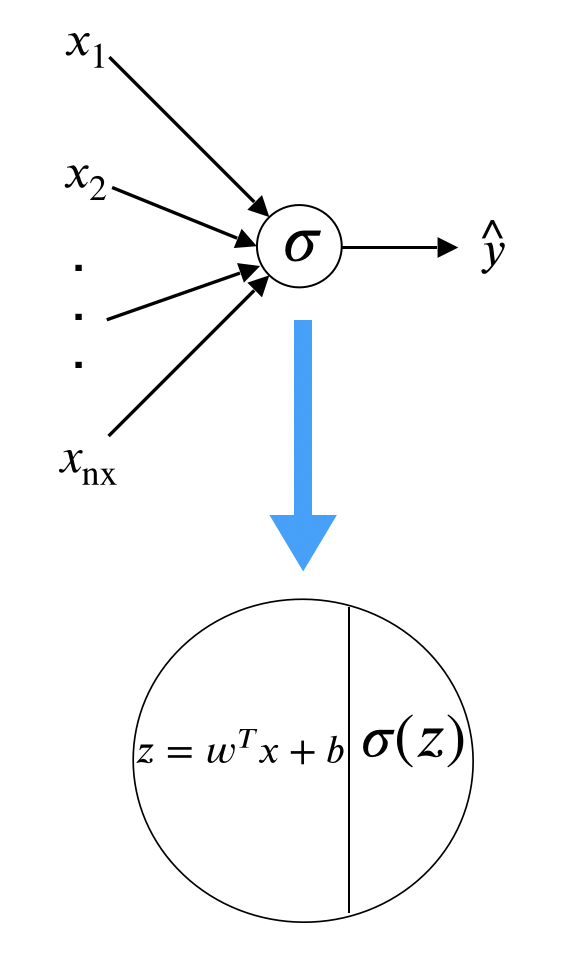
\includegraphics[width=0.30000\textwidth]{images/dnn0.png}

There are two types of layers. The last layer connects directly to the
output. All the rest are \emph{intermediate layers}. Depending on your
definition, we call it ``0-layer neural network'' where the layer count
only considers \emph{intermediate layers}. To train the model, you need
a cost function which is defined as equation \eqref{eq:costlogistic}.

\begin{equation}
J(w,b)=\frac{1}{m} \Sigma_{i=1}^m L(\hat{y}^{(i)}, y^{(i)}) = \frac{1}{m} \Sigma_{i=1}^{m} \{\ -y^{(i)}log(\hat{y}^{(i)})-(1-y^{(i)})log(1-\hat{y}^{(i)}) \}
\label{eq:costlogistic}
\end{equation}

The general approach to minimize \(J(w,b)\) is by gradient descent, also
known as \emph{back-propagation}. In logistic regression, it is easy to
calculate the gradient w.r.t the parameters \((w, b)\) using the chain
rule for differentiation. The optimization process is a forward and
backward sweep over the network. Let's look at the gradient descent for
logistic regression across m sample. The non-vectorized process is as
follows.

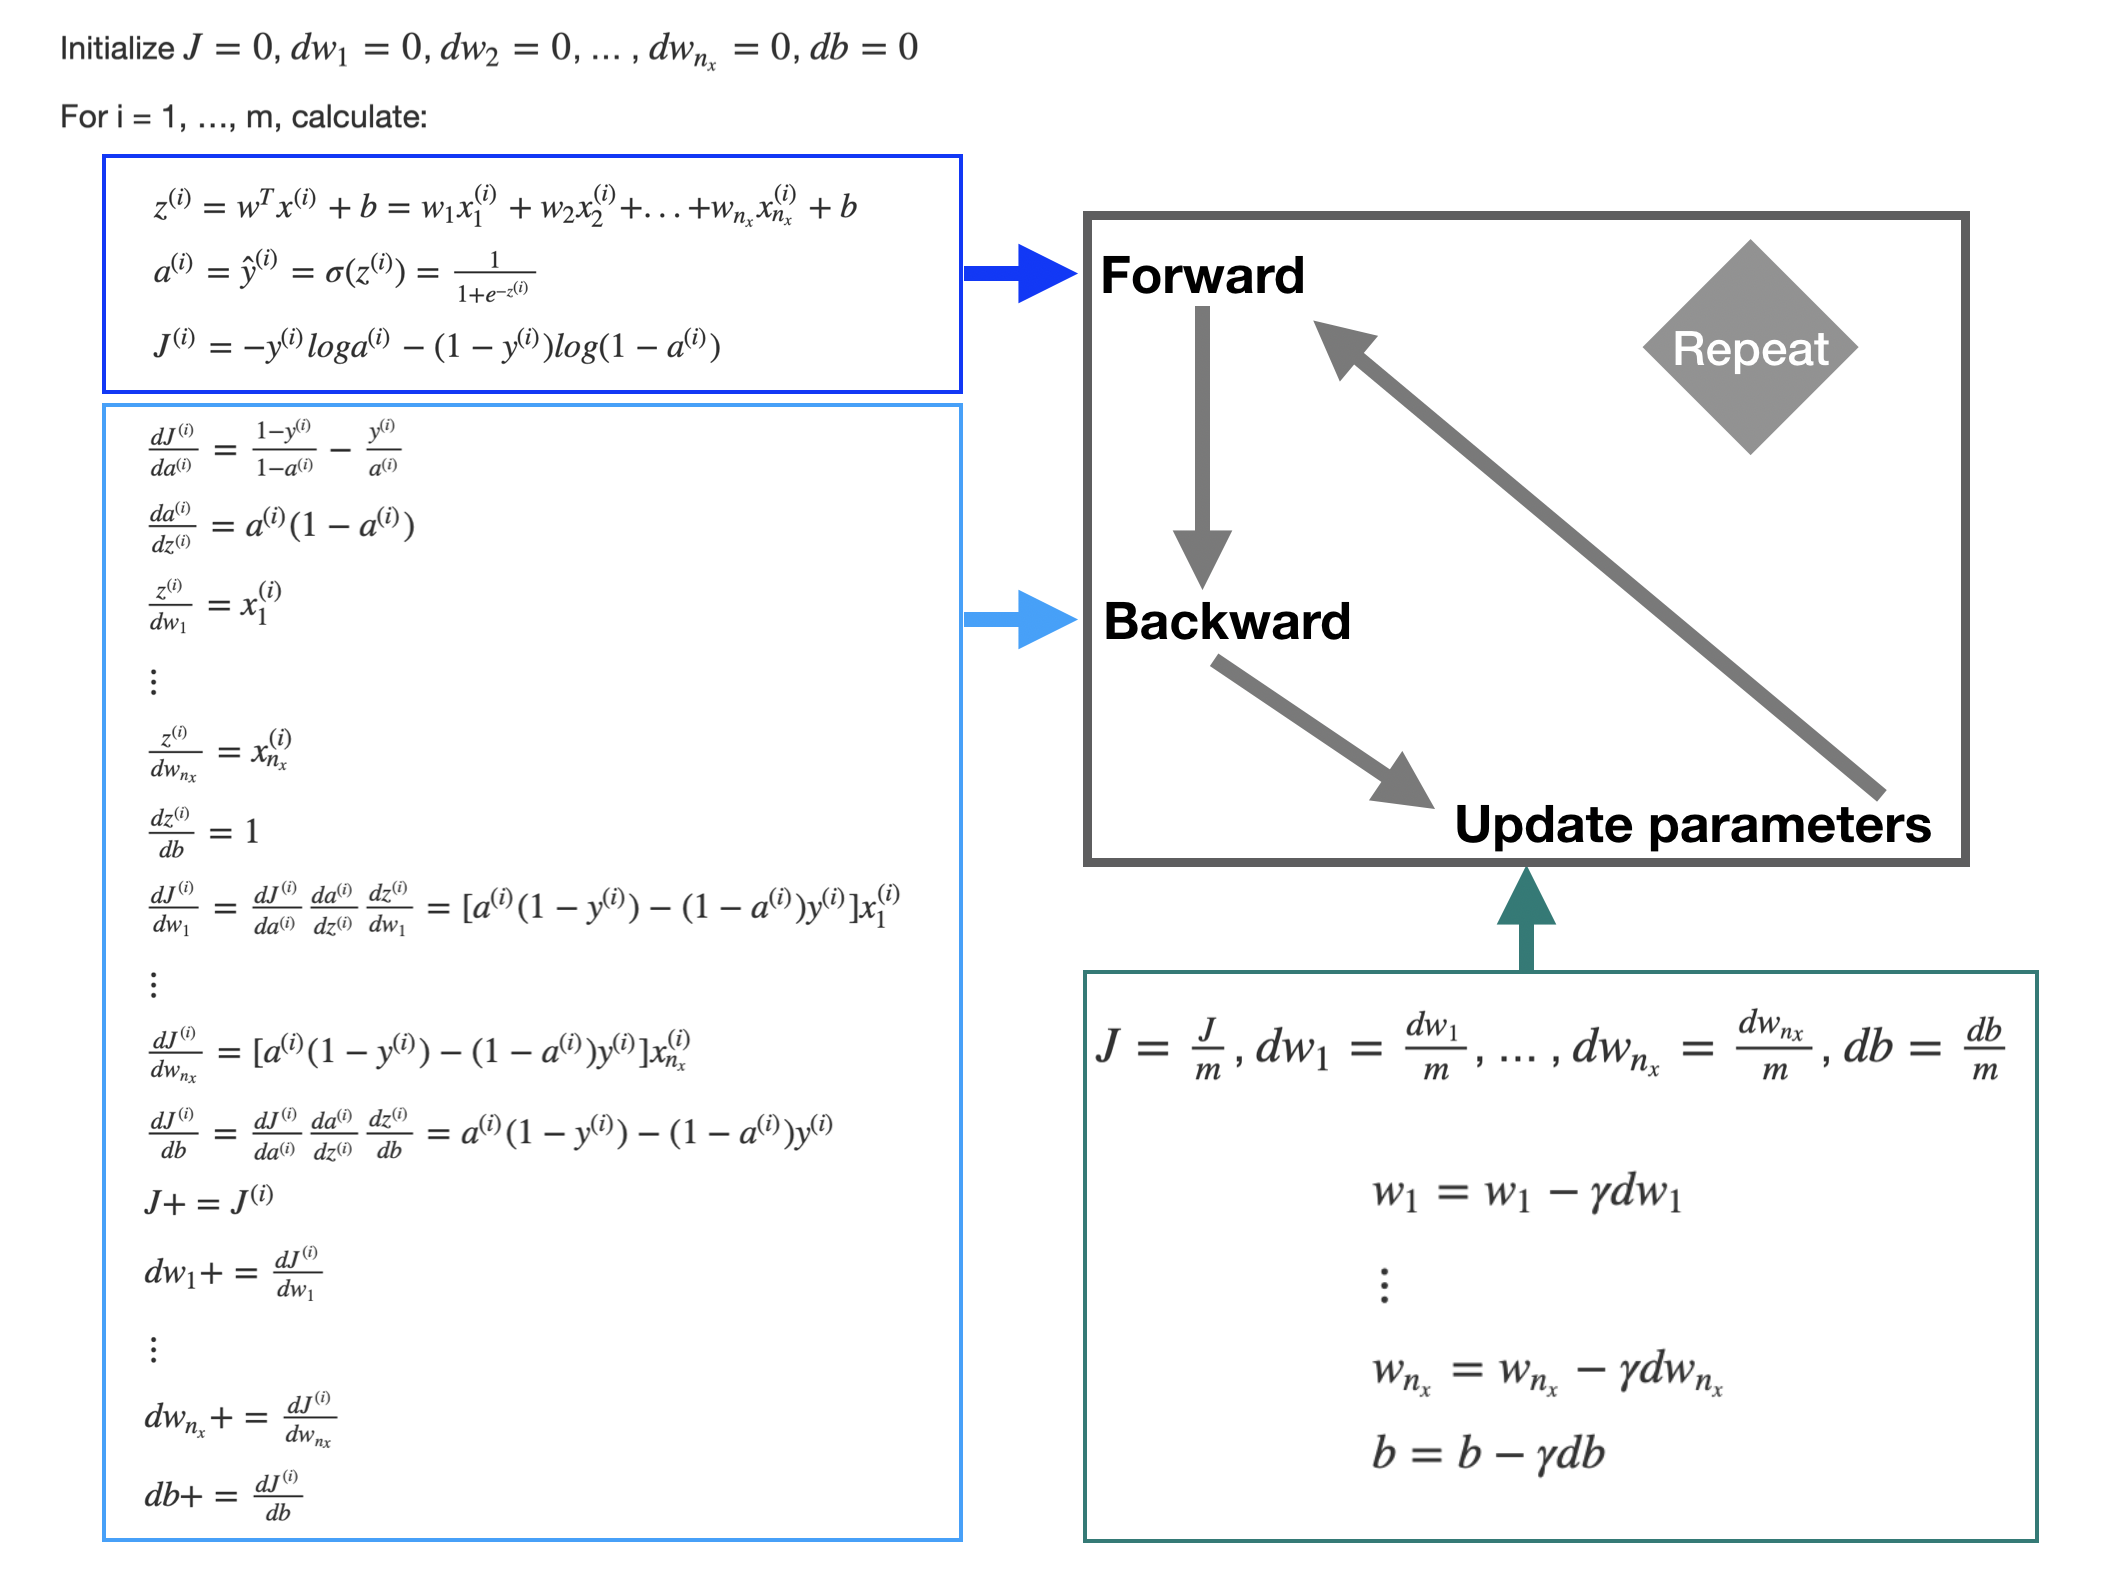
\includegraphics[width=1.00000\textwidth]{images/GradientDescent.png}

First initialize \(w_1\), \(w_2\), \ldots{} , \(w_{n_x}\), and \(b\).
Then plug in the initialized value to the forward and backward
propagation. The forward propagation takes the current weights and
calculates the prediction \(\hat{h}^{(i)}\) and cost \(J^{(i)}\). The
backward propagation calculates the gradient descent for the parameters.
After iterating through all \(m\) samples, you can calculate gradient
descent for the parameters. Then update the parameter by:
\[w := w - \gamma \frac{\partial J}{\partial w}\]
\[b := b - \gamma \frac{\partial J}{\partial b}\]

Repeat the progapation process using the updated parameter until the
cost \(J\) stabilizes.

\subsection{Deep Neural Network}\label{deep-neural-network}

Before people coined the term \emph{deep learning}, a neural network
refers to \emph{single hidden layer network}. Neural networks with more
than one layers are called \emph{deep learning}.

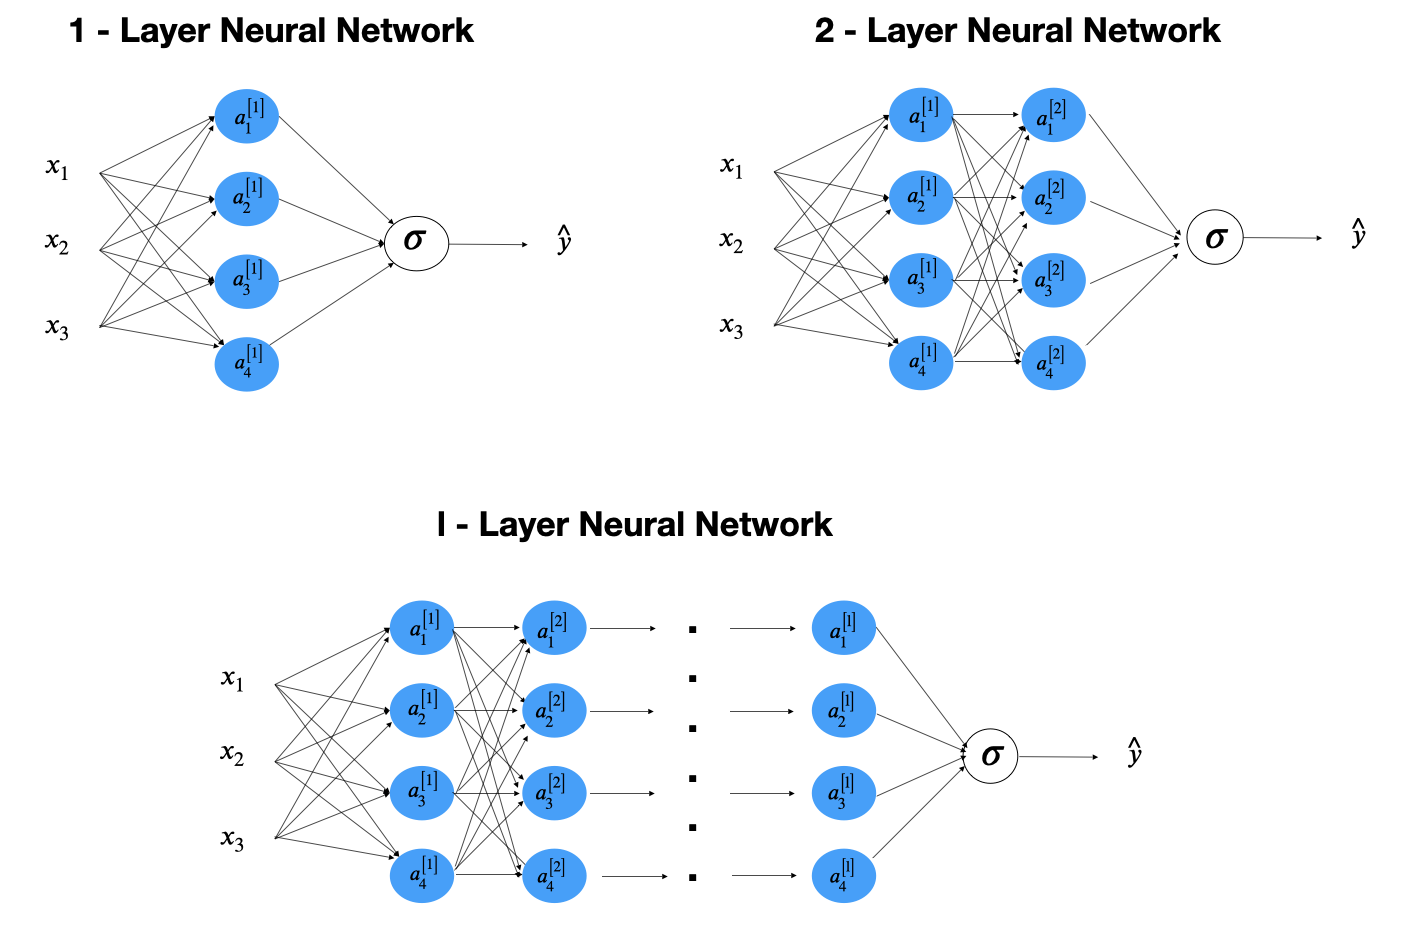
\includegraphics{images/dnn_str.png}

\subsection{Activation Function}\label{activation-function}

You need to choose activation function in the hidden layers. Logistic
regression only uses sigmoid activation function. But there are other
choices. Intermediate layers usually use different activation function
than the last layer. Let's first look at some of the common options
other than sigmoid.

\section{Convolutional Neural
Network}\label{convolutional-neural-network}

\section{Recurrent Neural Network}\label{recurrent-neural-network}

\appendix \addcontentsline{toc}{chapter}{\appendixname}


\chapter{Big Data Cloud Platform}\label{big-data-cloud-platform}

\section{How Data becomes Science?}\label{how-data-becomes-science}

Data has been statistician's friend for hundreds of years. Tabulated
data are the most familiar format that we use daily. People used to
store data on papers, tapes, diskettes, or hard drives. Only recently,
with the development of the computer, hardware, software, and
algorithms, the volume, variety, and speed of the data suddenly beyond
the capacity of a traditional statistician. And data becomes a special
science with the very first focus on a fundamental question: with a huge
amount of data, how can we store the data and quick access and process
the data. In the past a few years, by utilizing commodity hardware and
open source software, a big data ecosystem was created for data storage,
data retrieval, and parallel computation. Hadoop and Spark have become a
popular platform that enables data scientist, statistician, and business
analyst to access the data and to build models. Programming skills in
the big data platform have been the largest gap for a statistician to
become a successful data scientist. However, with the recent wave of
cloud computing, this gap is significantly reduced. Many of the
technical details have been pushed to the background, and the user
interface becomes much easier to learn. Cloud systems also enable quick
implementation to the production environment. Now data science is
emphasis more on the data itself as well as models and algorithms on top
of the data instead of platform and infrastructure.

\section{Power of Cluster of
Computers}\label{power-of-cluster-of-computers}

We are all familiar with our laptop/desktop computers which contain
mainly three components to finish computation with data: (1) Hard disk,
(2) Memory, and (3) CPU as shown in Figure 41 left. The data and codes
are stored in the hard disk which has certain features such as
relatively slow for reading and writes and relatively large capacity of
around a few TB in today's market. Memory is relatively fast for reading
and writing but relatively small in capacity in the order of a few
dozens of GB in today's market. CPU is where all the computation is
done.

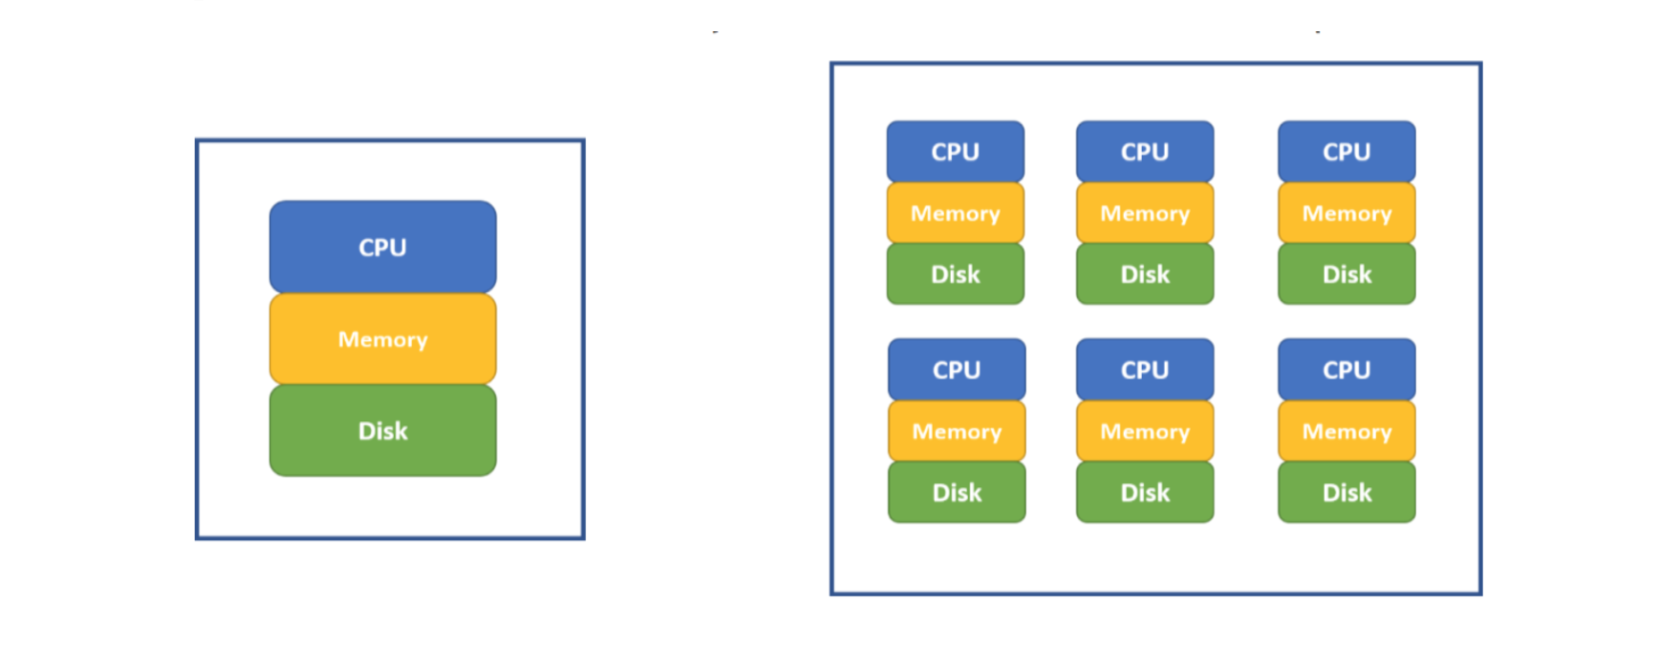
\includegraphics{images/cluster.png}

For statistical software such as R, the amount of data that it can
process is limited by the computer's memory. For a typical computer
before the year 2000, the memory is less than 1 GB. The memory capacity
grows far slower than the availability of the data to analyze. Now it is
quite often that we need to analyze data far beyond the capacity of a
single computer's memory, especially in an enterprise environment.
Meanwhile, the computation time is growing faster than linear to solve
the same problem (such as regressions) as the data size increases. Using
a cluster of computers become a common way to solve big data problem. In
Figure 41 (right), a cluster of computers can be viewed as one powerful
machine with total memory, hard disk and CPU equivale to the sum of
individual computers. It is common to have thousands of nodes for a
cluster.

In the past, to use a cluster of computers, users must write code (such
as MPI) to take care of how data is distributed and how the computation
is done in a parallel fashion. Luckily with the recent new development,
the cloud environment for big data analysis is more user-friendly. As
data is typically beyond the size of one hard disk, the dataset itself
is stored across different nodes' hard disk (i.e.~the Hadoop system
mentioned below). When we perform analysis, we can assume the needed
data is already distributed across many node's memories in the cluster
and algorithm are parallel in nature to leverage corresponding nodes'
CPUs to compute (i.e.~the Spark system mentioned below).

\subsection{Evolution of Clustering
Computing}\label{evolution-of-clustering-computing}

Using computer clusters to solve general purpose data and analytics
problems needs a lot of efforts if we have to specifically control every
element and steps such as data storage, memory allocation, and parallel
computation. Fortunately, high tech IT companies and open source
communities have developed the entire ecosystem based on Hadoop and
Spark. Users need only to know high-level scripting language such as
Python and R to leverage computer clusters' storage, memory and
computation power.

\subsection{Hadoop}\label{hadoop}

The very first problem internet companies face is that a lot of data has
been collected and how to better store these data for future analysis.
Google developed its own file system to provide efficient, reliable
access to data using large clusters of commodity hardware. The open
source version is known as Hadoop Distributed File System (HDFS). Both
systems use Map-Reduce to allocate computation across computation nodes
on top of the file system. Hadoop in written in Java and writing
map-reduce job using Java is a direct way to interact with Hadoop which
is not familiar to many in the data and analytics community. To help
better use Hadoop system, an SQL-like data warehouse system called Hive,
and a scripting language for analytics interface called Pig were
introduced for people with analytics background to interact with Hadoop
system. Within Hive, we can create user defined function through R or
Python to leverage the distributed and parallel computing
infrastructure. Map-reduce on top of HDFS is the main concept of the
Hadoop ecosystem. Each map-reduce operation requires retrieving data
from hard disk, computation time, and then storing the result onto disk
again. So, jobs on top of Hadoop require a lot of disk operation which
may slow down the computation process.

\subsection{Spark}\label{spark}

Spark works on top of distributed file system including HDFS with better
data and analytics efficiency by leveraging in-memory operations and is
more tailored for data processing and analytics. The spark system
includes an SQL-like framework called Spark SQL and a parallel machine
learning library called MLib. Fortunately for many in the analytics
community, Spark also supports R and Python. We can interact with data
stored in distributed file system using parallel computing across nodes
easily with R and Python through the Spark API and do not need to worry
about lower level details of distributed computing. We will introduce
how to use R notebook to drive Spark computations.

\section{Introduction of Cloud
Environment}\label{introduction-of-cloud-environment}

\chapter{Databases and SQL}\label{databases-and-sql}

\chapter{R code for data simulation}\label{r-code-for-data-simulation}

\section{Customer Data for Clothing
Company}\label{customer-data-for-clothing-company-1}

The simulation is not very straightforward and we will break it into
three parts:

\begin{enumerate}
\def\labelenumi{\arabic{enumi}.}
\tightlist
\item
  Define data structure: variable names, variable distribution, customer
  segment names, segment size
\item
  Variable distribution parameters: mean and variance
\item
  Iterate across segments and variables. Simulate data according to
  specific parameters assigned
\end{enumerate}

By organizing code this way, it makes easy for us to change specific
parts of the simulation. For example, if we want to change the
distribution of one variable, we can just change the corresponding part
of the code.

Here is code to define data structure:

\begin{Shaded}
\begin{Highlighting}[]
\CommentTok{# set a random number seed to make the process repeatable}
\KeywordTok{set.seed}\NormalTok{(}\DecValTok{12345}\NormalTok{)}
\CommentTok{# define the number of observations}
\NormalTok{ncust<-}\DecValTok{1000}
\CommentTok{# create a data frmae for simulated data}
\NormalTok{seg_dat<-}\KeywordTok{data.frame}\NormalTok{(}\DataTypeTok{id=}\KeywordTok{as.factor}\NormalTok{(}\KeywordTok{c}\NormalTok{(}\DecValTok{1}\OperatorTok{:}\NormalTok{ncust)))}
\CommentTok{# assign the variable names}
\NormalTok{vars<-}\KeywordTok{c}\NormalTok{(}\StringTok{"age"}\NormalTok{,}\StringTok{"gender"}\NormalTok{,}\StringTok{"income"}\NormalTok{,}\StringTok{"house"}\NormalTok{,}\StringTok{"store_exp"}\NormalTok{,}\StringTok{"online_exp"}\NormalTok{,}\StringTok{"store_trans"}\NormalTok{,}\StringTok{"online_trans"}\NormalTok{)}
\CommentTok{# assign distribution for each variable}
\NormalTok{vartype<-}\KeywordTok{c}\NormalTok{(}\StringTok{"norm"}\NormalTok{,}\StringTok{"binom"}\NormalTok{,}\StringTok{"norm"}\NormalTok{,}\StringTok{"binom"}\NormalTok{,}\StringTok{"norm"}\NormalTok{,}\StringTok{"norm"}\NormalTok{,}\StringTok{"pois"}\NormalTok{,}\StringTok{"pois"}\NormalTok{)}
\CommentTok{# names of 4 segments}
\NormalTok{group_name<-}\KeywordTok{c}\NormalTok{(}\StringTok{"Price"}\NormalTok{,}\StringTok{"Conspicuous"}\NormalTok{,}\StringTok{"Quality"}\NormalTok{,}\StringTok{"Style"}\NormalTok{)}
\CommentTok{# size of each segments}
\NormalTok{group_size<-}\KeywordTok{c}\NormalTok{(}\DecValTok{250}\NormalTok{,}\DecValTok{200}\NormalTok{,}\DecValTok{200}\NormalTok{,}\DecValTok{350}\NormalTok{)}
\end{Highlighting}
\end{Shaded}

The next step is to define variable distribution parameters. There are 4
segments of customers and 8 parameters. Different segments correspond to
different parameters. Let's store the parameters in a 4×8 matrix:

\begin{Shaded}
\begin{Highlighting}[]
\CommentTok{# matrix for mean}
\NormalTok{mus <-}\StringTok{ }\KeywordTok{matrix}\NormalTok{( }\KeywordTok{c}\NormalTok{(}
  \CommentTok{# Price}
  \DecValTok{60}\NormalTok{, }\FloatTok{0.5}\NormalTok{, }\DecValTok{120000}\NormalTok{,}\FloatTok{0.9}\NormalTok{, }\DecValTok{500}\NormalTok{,}\DecValTok{200}\NormalTok{,}\DecValTok{5}\NormalTok{,}\DecValTok{2}\NormalTok{,}
  \CommentTok{# Conspicuous}
  \DecValTok{40}\NormalTok{, }\FloatTok{0.7}\NormalTok{, }\DecValTok{200000}\NormalTok{,}\FloatTok{0.9}\NormalTok{, }\DecValTok{5000}\NormalTok{,}\DecValTok{5000}\NormalTok{,}\DecValTok{10}\NormalTok{,}\DecValTok{10}\NormalTok{,}
  \CommentTok{# Quality}
  \DecValTok{36}\NormalTok{, }\FloatTok{0.5}\NormalTok{, }\DecValTok{70000}\NormalTok{, }\FloatTok{0.4}\NormalTok{, }\DecValTok{300}\NormalTok{, }\DecValTok{2000}\NormalTok{,}\DecValTok{2}\NormalTok{,}\DecValTok{15}\NormalTok{,}
  \CommentTok{# Style}
  \DecValTok{25}\NormalTok{, }\FloatTok{0.2}\NormalTok{, }\DecValTok{90000}\NormalTok{, }\FloatTok{0.2}\NormalTok{, }\DecValTok{200}\NormalTok{, }\DecValTok{2000}\NormalTok{,}\DecValTok{2}\NormalTok{,}\DecValTok{20}\NormalTok{), }\DataTypeTok{ncol=}\KeywordTok{length}\NormalTok{(vars), }\DataTypeTok{byrow=}\OtherTok{TRUE}\NormalTok{)}
\end{Highlighting}
\end{Shaded}

\begin{Shaded}
\begin{Highlighting}[]
\CommentTok{# matrix for variance}
\NormalTok{sds<-}\StringTok{ }\KeywordTok{matrix}\NormalTok{( }\KeywordTok{c}\NormalTok{(}
  \CommentTok{# Price}
  \DecValTok{3}\NormalTok{,}\OtherTok{NA}\NormalTok{,}\DecValTok{8000}\NormalTok{,}\OtherTok{NA}\NormalTok{,}\DecValTok{100}\NormalTok{,}\DecValTok{50}\NormalTok{,}\OtherTok{NA}\NormalTok{,}\OtherTok{NA}\NormalTok{,}
  \CommentTok{# Conspicuous}
  \DecValTok{5}\NormalTok{,}\OtherTok{NA}\NormalTok{,}\DecValTok{50000}\NormalTok{,}\OtherTok{NA}\NormalTok{,}\DecValTok{1000}\NormalTok{,}\DecValTok{1500}\NormalTok{,}\OtherTok{NA}\NormalTok{,}\OtherTok{NA}\NormalTok{,}
  \CommentTok{# Quality}
  \DecValTok{7}\NormalTok{,}\OtherTok{NA}\NormalTok{,}\DecValTok{10000}\NormalTok{,}\OtherTok{NA}\NormalTok{,}\DecValTok{50}\NormalTok{,}\DecValTok{200}\NormalTok{,}\OtherTok{NA}\NormalTok{,}\OtherTok{NA}\NormalTok{,}
  \CommentTok{# Style}
  \DecValTok{2}\NormalTok{,}\OtherTok{NA}\NormalTok{,}\DecValTok{5000}\NormalTok{,}\OtherTok{NA}\NormalTok{,}\DecValTok{10}\NormalTok{,}\DecValTok{500}\NormalTok{,}\OtherTok{NA}\NormalTok{,}\OtherTok{NA}\NormalTok{), }\DataTypeTok{ncol=}\KeywordTok{length}\NormalTok{(vars), }\DataTypeTok{byrow=}\OtherTok{TRUE}\NormalTok{)}
\end{Highlighting}
\end{Shaded}

Now we are ready to simulate data using the parameters defined above:

\begin{Shaded}
\begin{Highlighting}[]
\CommentTok{# simulate non-survey data}
\NormalTok{sim.dat<-}\OtherTok{NULL}
\KeywordTok{set.seed}\NormalTok{(}\DecValTok{2016}\NormalTok{)}
\CommentTok{# loop on customer segment (i)}
 \ControlFlowTok{for}\NormalTok{ (i }\ControlFlowTok{in} \KeywordTok{seq_along}\NormalTok{(group_name))\{}
 
   \CommentTok{# add this line in order to moniter the process}
   \KeywordTok{cat}\NormalTok{ (i, group_name[i],}\StringTok{"}\CharTok{\textbackslash{}n}\StringTok{"}\NormalTok{)}
 
  \CommentTok{# create an empty matrix to store relevent data}
\NormalTok{  seg<-}\KeywordTok{data.frame}\NormalTok{(}\KeywordTok{matrix}\NormalTok{(}\OtherTok{NA}\NormalTok{,}\DataTypeTok{nrow=}\NormalTok{group_size[i], }\DataTypeTok{ncol=}\KeywordTok{length}\NormalTok{(vars)))  }
 
  \CommentTok{# Simulate data within segment i}
  \ControlFlowTok{for}\NormalTok{ (j }\ControlFlowTok{in} \KeywordTok{seq_along}\NormalTok{(vars))\{}
 
    \CommentTok{# loop on every variable (j)}
    \ControlFlowTok{if}\NormalTok{ (vartype[j]}\OperatorTok{==}\StringTok{"norm"}\NormalTok{)\{}
      \CommentTok{# simulate normal distribution}
\NormalTok{      seg[,j]<-}\KeywordTok{rnorm}\NormalTok{(group_size[i], }\DataTypeTok{mean=}\NormalTok{mus[i,j], }\DataTypeTok{sd=}\NormalTok{sds[i,j])}
\NormalTok{    \} }\ControlFlowTok{else} \ControlFlowTok{if}\NormalTok{ (vartype[j]}\OperatorTok{==}\StringTok{"pois"}\NormalTok{) \{}
      \CommentTok{# simulate poisson distribution}
\NormalTok{      seg[,j]<-}\KeywordTok{rpois}\NormalTok{(group_size[i], }\DataTypeTok{lambda=}\NormalTok{mus[i,j])}
\NormalTok{    \} }\ControlFlowTok{else} \ControlFlowTok{if}\NormalTok{ (vartype[j]}\OperatorTok{==}\StringTok{"binom"}\NormalTok{)\{}
      \CommentTok{# simulate binomial distribution}
\NormalTok{      seg[,j]<-}\KeywordTok{rbinom}\NormalTok{(group_size[i],}\DataTypeTok{size=}\DecValTok{1}\NormalTok{,}\DataTypeTok{prob=}\NormalTok{mus[i,j])}
\NormalTok{    \} }\ControlFlowTok{else}\NormalTok{\{}
      \CommentTok{# if the distribution name is not one of the above, stop and return a message}
      \KeywordTok{stop}\NormalTok{ (}\StringTok{"Don't have type:"}\NormalTok{,vartype[j])}
\NormalTok{    \}        }
\NormalTok{  \}}
\NormalTok{  sim.dat<-}\KeywordTok{rbind}\NormalTok{(sim.dat,seg)}
\NormalTok{ \}}
\end{Highlighting}
\end{Shaded}

Now let's edit the data we just simulated a little by adding tags to 0/1
binomial variables:

\begin{Shaded}
\begin{Highlighting}[]
\CommentTok{# assign variable names}
\KeywordTok{names}\NormalTok{(sim.dat)<-vars}
\CommentTok{# assign factor levels to segment variable}
\NormalTok{sim.dat}\OperatorTok{$}\NormalTok{segment<-}\KeywordTok{factor}\NormalTok{(}\KeywordTok{rep}\NormalTok{(group_name,}\DataTypeTok{times=}\NormalTok{group_size))}
\CommentTok{# recode gender and house variable}
\NormalTok{sim.dat}\OperatorTok{$}\NormalTok{gender<-}\KeywordTok{factor}\NormalTok{(sim.dat}\OperatorTok{$}\NormalTok{gender, }\DataTypeTok{labels=}\KeywordTok{c}\NormalTok{(}\StringTok{"Female"}\NormalTok{,}\StringTok{"Male"}\NormalTok{))}
\NormalTok{sim.dat}\OperatorTok{$}\NormalTok{house<-}\KeywordTok{factor}\NormalTok{(sim.dat}\OperatorTok{$}\NormalTok{house, }\DataTypeTok{labels=}\KeywordTok{c}\NormalTok{(}\StringTok{"No"}\NormalTok{,}\StringTok{"Yes"}\NormalTok{))}
\CommentTok{# store_trans and online_trans are at least 1}
\NormalTok{sim.dat}\OperatorTok{$}\NormalTok{store_trans<-sim.dat}\OperatorTok{$}\NormalTok{store_trans}\OperatorTok{+}\DecValTok{1}
\NormalTok{sim.dat}\OperatorTok{$}\NormalTok{online_trans<-sim.dat}\OperatorTok{$}\NormalTok{online_trans}\OperatorTok{+}\DecValTok{1}
\CommentTok{# age is integer}
\NormalTok{sim.dat}\OperatorTok{$}\NormalTok{age<-}\KeywordTok{floor}\NormalTok{(sim.dat}\OperatorTok{$}\NormalTok{age)}
\end{Highlighting}
\end{Shaded}

In the real world, the data always includes some noise such as missing,
wrong imputation. So we will add some noise to the data:

\begin{Shaded}
\begin{Highlighting}[]
\CommentTok{# add missing values}
\NormalTok{idxm <-}\StringTok{ }\KeywordTok{as.logical}\NormalTok{(}\KeywordTok{rbinom}\NormalTok{(ncust, }\DataTypeTok{size=}\DecValTok{1}\NormalTok{, }\DataTypeTok{prob=}\NormalTok{sim.dat}\OperatorTok{$}\NormalTok{age}\OperatorTok{/}\DecValTok{200}\NormalTok{))}
\NormalTok{sim.dat}\OperatorTok{$}\NormalTok{income[idxm]<-}\OtherTok{NA}
\CommentTok{# add wrong imputations and outliers}
\KeywordTok{set.seed}\NormalTok{(}\DecValTok{123}\NormalTok{)}
\NormalTok{idx<-}\KeywordTok{sample}\NormalTok{(}\DecValTok{1}\OperatorTok{:}\NormalTok{ncust,}\DecValTok{5}\NormalTok{)}
\NormalTok{sim.dat}\OperatorTok{$}\NormalTok{age[idx[}\DecValTok{1}\NormalTok{]]<-}\DecValTok{300}
\NormalTok{sim.dat}\OperatorTok{$}\NormalTok{store_exp[idx[}\DecValTok{2}\NormalTok{]]<-}\StringTok{ }\OperatorTok{-}\DecValTok{500}
\NormalTok{sim.dat}\OperatorTok{$}\NormalTok{store_exp[idx[}\DecValTok{3}\OperatorTok{:}\DecValTok{5}\NormalTok{]]<-}\KeywordTok{c}\NormalTok{(}\DecValTok{50000}\NormalTok{,}\DecValTok{30000}\NormalTok{,}\DecValTok{30000}\NormalTok{)}
\end{Highlighting}
\end{Shaded}

So far we have created part of the data. You can check it using
\texttt{summary(sim.dat)}. Next, we will move on to simulate survey
data.

\begin{Shaded}
\begin{Highlighting}[]
\CommentTok{# number of survey questions}
\NormalTok{nq<-}\DecValTok{10}
\CommentTok{# mean matrix for different segments }
\NormalTok{mus2 <-}\StringTok{ }\KeywordTok{matrix}\NormalTok{( }\KeywordTok{c}\NormalTok{(}
  \CommentTok{# Price}
 \DecValTok{5}\NormalTok{,}\DecValTok{2}\NormalTok{,}\DecValTok{1}\NormalTok{,}\DecValTok{3}\NormalTok{,}\DecValTok{1}\NormalTok{,}\DecValTok{4}\NormalTok{,}\DecValTok{1}\NormalTok{,}\DecValTok{4}\NormalTok{,}\DecValTok{2}\NormalTok{,}\DecValTok{4}\NormalTok{,}
  \CommentTok{# Conspicuous}
 \DecValTok{1}\NormalTok{,}\DecValTok{4}\NormalTok{,}\DecValTok{5}\NormalTok{,}\DecValTok{4}\NormalTok{,}\DecValTok{4}\NormalTok{,}\DecValTok{4}\NormalTok{,}\DecValTok{4}\NormalTok{,}\DecValTok{1}\NormalTok{,}\DecValTok{4}\NormalTok{,}\DecValTok{2}\NormalTok{,}
  \CommentTok{# Quality}
 \DecValTok{5}\NormalTok{,}\DecValTok{2}\NormalTok{,}\DecValTok{3}\NormalTok{,}\DecValTok{4}\NormalTok{,}\DecValTok{3}\NormalTok{,}\DecValTok{2}\NormalTok{,}\DecValTok{4}\NormalTok{,}\DecValTok{2}\NormalTok{,}\DecValTok{3}\NormalTok{,}\DecValTok{3}\NormalTok{,}
  \CommentTok{# Style}
 \DecValTok{3}\NormalTok{,}\DecValTok{1}\NormalTok{,}\DecValTok{1}\NormalTok{,}\DecValTok{2}\NormalTok{,}\DecValTok{4}\NormalTok{,}\DecValTok{1}\NormalTok{,}\DecValTok{5}\NormalTok{,}\DecValTok{3}\NormalTok{,}\DecValTok{4}\NormalTok{,}\DecValTok{2}\NormalTok{), }\DataTypeTok{ncol=}\NormalTok{nq, }\DataTypeTok{byrow=}\OtherTok{TRUE}\NormalTok{)}

\CommentTok{# assume the variance is 0.2 for all}
\NormalTok{sd2<-}\FloatTok{0.2}
\NormalTok{sim.dat2<-}\OtherTok{NULL}
\KeywordTok{set.seed}\NormalTok{(}\DecValTok{1000}\NormalTok{)}
\CommentTok{# loop for customer segment (i)}
\ControlFlowTok{for}\NormalTok{ (i }\ControlFlowTok{in} \KeywordTok{seq_along}\NormalTok{(group_name))\{}
  \CommentTok{# the following line is used for checking the progress}
  \CommentTok{# cat (i, group_name[i],"\textbackslash{}n")}
  \CommentTok{# create an empty data frame to store data}
\NormalTok{  seg<-}\KeywordTok{data.frame}\NormalTok{(}\KeywordTok{matrix}\NormalTok{(}\OtherTok{NA}\NormalTok{,}\DataTypeTok{nrow=}\NormalTok{group_size[i], }\DataTypeTok{ncol=}\NormalTok{nq))  }
  \CommentTok{# simulate data within segment}
  \ControlFlowTok{for}\NormalTok{ (j }\ControlFlowTok{in} \DecValTok{1}\OperatorTok{:}\NormalTok{nq)\{}
    \CommentTok{# simulate normal distribution}
\NormalTok{    res<-}\KeywordTok{rnorm}\NormalTok{(group_size[i], }\DataTypeTok{mean=}\NormalTok{mus2[i,j], }\DataTypeTok{sd=}\NormalTok{sd2)}
    \CommentTok{# set upper and lower limit}
\NormalTok{    res[res}\OperatorTok{>}\DecValTok{5}\NormalTok{]<-}\DecValTok{5}
\NormalTok{    res[res}\OperatorTok{<}\DecValTok{1}\NormalTok{]<-}\DecValTok{1}
    \CommentTok{# convert continuous values to discrete integers}
\NormalTok{    seg[,j]<-}\KeywordTok{floor}\NormalTok{(res)}
\NormalTok{  \}}
\NormalTok{  sim.dat2<-}\KeywordTok{rbind}\NormalTok{(sim.dat2,seg)}
\NormalTok{\}}

\KeywordTok{names}\NormalTok{(sim.dat2)<-}\KeywordTok{paste}\NormalTok{(}\StringTok{"Q"}\NormalTok{,}\DecValTok{1}\OperatorTok{:}\DecValTok{10}\NormalTok{,}\DataTypeTok{sep=}\StringTok{""}\NormalTok{)}
\NormalTok{sim.dat<-}\KeywordTok{cbind}\NormalTok{(sim.dat,sim.dat2)}
\NormalTok{sim.dat}\OperatorTok{$}\NormalTok{segment<-}\KeywordTok{factor}\NormalTok{(}\KeywordTok{rep}\NormalTok{(group_name,}\DataTypeTok{times=}\NormalTok{group_size))}
\end{Highlighting}
\end{Shaded}

\section{Customer Satisfaction Survey Data from Airline
Company}\label{customer-satisfaction-survey-data-from-airline-company-1}

\begin{Shaded}
\begin{Highlighting}[]
\CommentTok{# Create a matrix of factor loadings}
\CommentTok{# This pattern is called bifactor because it has a general factor for separate components.}
\CommentTok{# For example, "Ease of making reservation" has general factor loading 0.33, specific factor loading 0.58}
\CommentTok{# The outcome variables are formed as combinations of these general and specific factors}
\NormalTok{loadings <-}\StringTok{ }\KeywordTok{matrix}\NormalTok{(}\KeywordTok{c}\NormalTok{ (}
  \CommentTok{# Ticketing}
\NormalTok{  .}\DecValTok{33}\NormalTok{, .}\DecValTok{58}\NormalTok{, .}\DecValTok{00}\NormalTok{, .}\DecValTok{00}\NormalTok{,  }\CommentTok{# Ease of making reservation }
\NormalTok{  .}\DecValTok{35}\NormalTok{, .}\DecValTok{55}\NormalTok{, .}\DecValTok{00}\NormalTok{, .}\DecValTok{00}\NormalTok{,  }\CommentTok{# Availability of preferred seats}
\NormalTok{  .}\DecValTok{30}\NormalTok{, .}\DecValTok{52}\NormalTok{, .}\DecValTok{00}\NormalTok{, .}\DecValTok{00}\NormalTok{,  }\CommentTok{# Variety of flight options}
\NormalTok{  .}\DecValTok{40}\NormalTok{, .}\DecValTok{50}\NormalTok{, .}\DecValTok{00}\NormalTok{, .}\DecValTok{00}\NormalTok{,  }\CommentTok{# Ticket prices}
  \CommentTok{# Aircraft}
\NormalTok{  .}\DecValTok{50}\NormalTok{, .}\DecValTok{00}\NormalTok{, .}\DecValTok{55}\NormalTok{, .}\DecValTok{00}\NormalTok{,  }\CommentTok{# Seat comfort}
\NormalTok{  .}\DecValTok{41}\NormalTok{, .}\DecValTok{00}\NormalTok{, .}\DecValTok{51}\NormalTok{, .}\DecValTok{00}\NormalTok{,  }\CommentTok{# Roominess of seat area}
\NormalTok{  .}\DecValTok{45}\NormalTok{, .}\DecValTok{00}\NormalTok{, .}\DecValTok{57}\NormalTok{, .}\DecValTok{00}\NormalTok{,  }\CommentTok{# Availability of Overhead}
\NormalTok{  .}\DecValTok{32}\NormalTok{, .}\DecValTok{00}\NormalTok{, .}\DecValTok{54}\NormalTok{, .}\DecValTok{00}\NormalTok{,  }\CommentTok{# Cleanliness of aircraft}
  \CommentTok{# Service}
\NormalTok{  .}\DecValTok{35}\NormalTok{, .}\DecValTok{00}\NormalTok{, .}\DecValTok{00}\NormalTok{, .}\DecValTok{50}\NormalTok{,  }\CommentTok{# Courtesy of flight attendant}
\NormalTok{  .}\DecValTok{38}\NormalTok{, .}\DecValTok{00}\NormalTok{, .}\DecValTok{00}\NormalTok{, .}\DecValTok{57}\NormalTok{,  }\CommentTok{# Friendliness}
\NormalTok{  .}\DecValTok{60}\NormalTok{, .}\DecValTok{00}\NormalTok{, .}\DecValTok{00}\NormalTok{, .}\DecValTok{50}\NormalTok{,  }\CommentTok{# Helpfulness}
\NormalTok{  .}\DecValTok{52}\NormalTok{, .}\DecValTok{00}\NormalTok{, .}\DecValTok{00}\NormalTok{, .}\DecValTok{58}\NormalTok{,  }\CommentTok{# Food and drinks}
  \CommentTok{# General   }
\NormalTok{  .}\DecValTok{43}\NormalTok{, .}\DecValTok{10}\NormalTok{, .}\DecValTok{30}\NormalTok{, .}\DecValTok{30}\NormalTok{,  }\CommentTok{# Overall satisfaction}
\NormalTok{  .}\DecValTok{35}\NormalTok{, .}\DecValTok{50}\NormalTok{, .}\DecValTok{40}\NormalTok{, .}\DecValTok{20}\NormalTok{,  }\CommentTok{# Purchase again}
\NormalTok{  .}\DecValTok{25}\NormalTok{, .}\DecValTok{50}\NormalTok{, .}\DecValTok{50}\NormalTok{, .}\DecValTok{20}\NormalTok{), }\CommentTok{# Willingness to recommend}
  \DataTypeTok{nrow=}\DecValTok{15}\NormalTok{,}\DataTypeTok{ncol=}\DecValTok{4}\NormalTok{, }\DataTypeTok{byrow=}\OtherTok{TRUE}\NormalTok{)}
  
\CommentTok{# Matrix multiplication produces the correlation matrix except for the diagonal}
\NormalTok{cor_matrix<-loadings }\OperatorTok\StringTok{ }\KeywordTok{t}\NormalTok{(loadings)}
\CommentTok{# Diagonal set to ones}
\KeywordTok{diag}\NormalTok{(cor_matrix)<-}\DecValTok{1}

\CommentTok{# use the mvtnorm package to randomly generate a data set with a given correlation pattern}

\KeywordTok{library}\NormalTok{(mvtnorm)}
\CommentTok{# mean vectors of the 3 airline companies}
\NormalTok{mu1=}\KeywordTok{c}\NormalTok{(}\DecValTok{5}\NormalTok{,}\DecValTok{6}\NormalTok{,}\DecValTok{5}\NormalTok{,}\DecValTok{6}\NormalTok{, }\DecValTok{7}\NormalTok{,}\DecValTok{8}\NormalTok{,}\DecValTok{6}\NormalTok{,}\DecValTok{7}\NormalTok{, }\DecValTok{5}\NormalTok{,}\DecValTok{5}\NormalTok{,}\DecValTok{5}\NormalTok{,}\DecValTok{5}\NormalTok{, }\DecValTok{6}\NormalTok{,}\DecValTok{6}\NormalTok{,}\DecValTok{6}\NormalTok{)}
\NormalTok{mu2=}\KeywordTok{c}\NormalTok{(}\DecValTok{3}\NormalTok{,}\DecValTok{3}\NormalTok{,}\DecValTok{2}\NormalTok{,}\DecValTok{3}\NormalTok{, }\DecValTok{5}\NormalTok{,}\DecValTok{4}\NormalTok{,}\DecValTok{5}\NormalTok{,}\DecValTok{6}\NormalTok{, }\DecValTok{8}\NormalTok{,}\DecValTok{8}\NormalTok{,}\DecValTok{8}\NormalTok{,}\DecValTok{8}\NormalTok{, }\DecValTok{3}\NormalTok{,}\DecValTok{3}\NormalTok{,}\DecValTok{3}\NormalTok{)}
\NormalTok{mu3=}\KeywordTok{c}\NormalTok{(}\DecValTok{2}\NormalTok{,}\DecValTok{2}\NormalTok{,}\DecValTok{2}\NormalTok{,}\DecValTok{2}\NormalTok{, }\DecValTok{8}\NormalTok{,}\DecValTok{8}\NormalTok{,}\DecValTok{8}\NormalTok{,}\DecValTok{8}\NormalTok{, }\DecValTok{8}\NormalTok{,}\DecValTok{8}\NormalTok{,}\DecValTok{8}\NormalTok{,}\DecValTok{8}\NormalTok{, }\DecValTok{8}\NormalTok{,}\DecValTok{8}\NormalTok{,}\DecValTok{8}\NormalTok{)}

\CommentTok{# set random seed}
\KeywordTok{set.seed}\NormalTok{(}\DecValTok{123456}\NormalTok{) }
\CommentTok{# respondent ID}
\NormalTok{resp.id <-}\StringTok{ }\DecValTok{1}\OperatorTok{:}\DecValTok{1000} 

\KeywordTok{library}\NormalTok{(MASS) }
\NormalTok{rating1 <-}\StringTok{ }\KeywordTok{mvrnorm}\NormalTok{(}\KeywordTok{length}\NormalTok{(resp.id),}
                     \DataTypeTok{mu=}\NormalTok{mu1,}
                     \DataTypeTok{Sigma=}\NormalTok{cor_matrix)}
\NormalTok{rating2 <-}\StringTok{ }\KeywordTok{mvrnorm}\NormalTok{(}\KeywordTok{length}\NormalTok{(resp.id),}
                   \DataTypeTok{mu=}\NormalTok{mu2,}
                   \DataTypeTok{Sigma=}\NormalTok{cor_matrix)}
\NormalTok{rating3 <-}\StringTok{ }\KeywordTok{mvrnorm}\NormalTok{(}\KeywordTok{length}\NormalTok{(resp.id),}
                   \DataTypeTok{mu=}\NormalTok{mu3,}
                   \DataTypeTok{Sigma=}\NormalTok{cor_matrix)}


\CommentTok{# truncates scale to be between 1 and 9}
\NormalTok{rating1[rating1}\OperatorTok{>}\DecValTok{9}\NormalTok{]<-}\DecValTok{9}
\NormalTok{rating1[rating1}\OperatorTok{<}\DecValTok{1}\NormalTok{]<-}\DecValTok{1}
\NormalTok{rating2[rating2}\OperatorTok{>}\DecValTok{9}\NormalTok{]<-}\DecValTok{9}
\NormalTok{rating2[rating2}\OperatorTok{<}\DecValTok{1}\NormalTok{]<-}\DecValTok{1}
\NormalTok{rating3[rating3}\OperatorTok{>}\DecValTok{9}\NormalTok{]<-}\DecValTok{9}
\NormalTok{rating3[rating3}\OperatorTok{<}\DecValTok{1}\NormalTok{]<-}\DecValTok{1}

\CommentTok{# Round to single digit}
\NormalTok{rating1<-}\KeywordTok{data.frame}\NormalTok{(}\KeywordTok{round}\NormalTok{(rating1,}\DecValTok{0}\NormalTok{))}
\NormalTok{rating2<-}\KeywordTok{data.frame}\NormalTok{(}\KeywordTok{round}\NormalTok{(rating2,}\DecValTok{0}\NormalTok{))}
\NormalTok{rating3<-}\KeywordTok{data.frame}\NormalTok{(}\KeywordTok{round}\NormalTok{(rating3,}\DecValTok{0}\NormalTok{))}
\NormalTok{rating1}\OperatorTok{$}\NormalTok{ID<-resp.id}
\NormalTok{rating2}\OperatorTok{$}\NormalTok{ID<-resp.id}
\NormalTok{rating3}\OperatorTok{$}\NormalTok{ID<-resp.id}
\NormalTok{rating1}\OperatorTok{$}\NormalTok{Airline<-}\KeywordTok{rep}\NormalTok{(}\StringTok{"AirlineCo.1"}\NormalTok{,}\KeywordTok{length}\NormalTok{(resp.id))}
\NormalTok{rating2}\OperatorTok{$}\NormalTok{Airline<-}\KeywordTok{rep}\NormalTok{(}\StringTok{"AirlineCo.2"}\NormalTok{,}\KeywordTok{length}\NormalTok{(resp.id))}
\NormalTok{rating3}\OperatorTok{$}\NormalTok{Airline<-}\KeywordTok{rep}\NormalTok{(}\StringTok{"AirlineCo.3"}\NormalTok{,}\KeywordTok{length}\NormalTok{(resp.id))}
\NormalTok{rating<-}\KeywordTok{rbind}\NormalTok{(rating1,rating2,rating3)}

\CommentTok{# assign names to the variables in the data frame}
\KeywordTok{names}\NormalTok{(rating)<-}\KeywordTok{c}\NormalTok{(}
  \StringTok{"Easy_Reservation"}\NormalTok{,}
  \StringTok{"Preferred_Seats"}\NormalTok{,}
  \StringTok{"Flight_Options"}\NormalTok{,}
  \StringTok{"Ticket_Prices"}\NormalTok{,}
  \StringTok{"Seat_Comfort"}\NormalTok{,}
  \StringTok{"Seat_Roominess"}\NormalTok{,}
  \StringTok{"Overhead_Storage"}\NormalTok{,}
  \StringTok{"Clean_Aircraft"}\NormalTok{,}
  \StringTok{"Courtesy"}\NormalTok{,}
  \StringTok{"Friendliness"}\NormalTok{,}
  \StringTok{"Helpfulness"}\NormalTok{,}
  \StringTok{"Service"}\NormalTok{,}
  \StringTok{"Satisfaction"}\NormalTok{,}
  \StringTok{"Fly_Again"}\NormalTok{,}
  \StringTok{"Recommend"}\NormalTok{,}
  \StringTok{"ID"}\NormalTok{,}
  \StringTok{"Airline"}\NormalTok{)}
\end{Highlighting}
\end{Shaded}

\section{Swine Disease Breakout
Data}\label{swine-disease-breakout-data-1}

\begin{Shaded}
\begin{Highlighting}[]
\CommentTok{# sim1_da1.csv the 1st simulated data similar sim1_da2 and sim1_da3}
\CommentTok{# sim1.csv simulated data, the first simulation dummy.sim1.csv dummy}
\CommentTok{# variables for the first simulated data with all the baseline code for}
\CommentTok{# simulation}

\CommentTok{# setwd(dirname(file.choose())) library(grplasso)}

\NormalTok{nf <-}\StringTok{ }\DecValTok{800}
\ControlFlowTok{for}\NormalTok{ (j }\ControlFlowTok{in} \DecValTok{1}\OperatorTok{:}\DecValTok{20}\NormalTok{) \{}
    \KeywordTok{set.seed}\NormalTok{(}\DecValTok{19870} \OperatorTok{+}\StringTok{ }\NormalTok{j)}
\NormalTok{    x <-}\StringTok{ }\KeywordTok{c}\NormalTok{(}\StringTok{"A"}\NormalTok{, }\StringTok{"B"}\NormalTok{, }\StringTok{"C"}\NormalTok{)}
\NormalTok{    sim.da1 <-}\StringTok{ }\OtherTok{NULL}
    \ControlFlowTok{for}\NormalTok{ (i }\ControlFlowTok{in} \DecValTok{1}\OperatorTok{:}\NormalTok{nf) \{}
        \CommentTok{# sample(x, 120, replace=TRUE)->sam}
\NormalTok{        sim.da1 <-}\StringTok{ }\KeywordTok{rbind}\NormalTok{(sim.da1, }\KeywordTok{sample}\NormalTok{(x, }\DecValTok{120}\NormalTok{, }\DataTypeTok{replace =} \OtherTok{TRUE}\NormalTok{))}
\NormalTok{    \}}
    
\NormalTok{    sim.da1 <-}\StringTok{ }\KeywordTok{data.frame}\NormalTok{(sim.da1)}
\NormalTok{    col <-}\StringTok{ }\KeywordTok{paste}\NormalTok{(}\StringTok{"Q"}\NormalTok{, }\DecValTok{1}\OperatorTok{:}\DecValTok{120}\NormalTok{, }\DataTypeTok{sep =} \StringTok{""}\NormalTok{)}
\NormalTok{    row <-}\StringTok{ }\KeywordTok{paste}\NormalTok{(}\StringTok{"Farm"}\NormalTok{, }\DecValTok{1}\OperatorTok{:}\NormalTok{nf, }\DataTypeTok{sep =} \StringTok{""}\NormalTok{)}
    \KeywordTok{colnames}\NormalTok{(sim.da1) <-}\StringTok{ }\NormalTok{col}
    \KeywordTok{rownames}\NormalTok{(sim.da1) <-}\StringTok{ }\NormalTok{row}
    
    \CommentTok{# use class.ind() function in nnet package to encode dummy variables}
    \KeywordTok{library}\NormalTok{(nnet)}
\NormalTok{    dummy.sim1 <-}\StringTok{ }\OtherTok{NULL}
    \ControlFlowTok{for}\NormalTok{ (k }\ControlFlowTok{in} \DecValTok{1}\OperatorTok{:}\KeywordTok{ncol}\NormalTok{(sim.da1)) \{}
\NormalTok{        tmp =}\StringTok{ }\KeywordTok{class.ind}\NormalTok{(sim.da1[, k])}
        \KeywordTok{colnames}\NormalTok{(tmp) =}\StringTok{ }\KeywordTok{paste}\NormalTok{(col[k], }\KeywordTok{colnames}\NormalTok{(tmp))}
\NormalTok{        dummy.sim1 =}\StringTok{ }\KeywordTok{cbind}\NormalTok{(dummy.sim1, tmp)}
\NormalTok{    \}}
\NormalTok{    dummy.sim1 <-}\StringTok{ }\KeywordTok{data.frame}\NormalTok{(dummy.sim1)}
    
    \CommentTok{# set 'C' as the baseline delete baseline dummy variable}
    
\NormalTok{    base.idx <-}\StringTok{ }\DecValTok{3} \OperatorTok{*}\StringTok{ }\KeywordTok{c}\NormalTok{(}\DecValTok{1}\OperatorTok{:}\DecValTok{120}\NormalTok{)}
\NormalTok{    dummy1 <-}\StringTok{ }\NormalTok{dummy.sim1[, }\OperatorTok{-}\NormalTok{base.idx]}
    
    \CommentTok{# simulate independent variable for different values of r simulate}
    \CommentTok{# based on one value of r each time r=0.1, get the link function}
\NormalTok{    s1 <-}\StringTok{ }\KeywordTok{c}\NormalTok{(}\KeywordTok{rep}\NormalTok{(}\KeywordTok{c}\NormalTok{(}\DecValTok{1}\OperatorTok{/}\DecValTok{10}\NormalTok{, }\DecValTok{0}\NormalTok{, }\OperatorTok{-}\DecValTok{1}\OperatorTok{/}\DecValTok{10}\NormalTok{), }\DecValTok{40}\NormalTok{), }\KeywordTok{rep}\NormalTok{(}\KeywordTok{c}\NormalTok{(}\DecValTok{1}\OperatorTok{/}\DecValTok{10}\NormalTok{, }\DecValTok{0}\NormalTok{, }\DecValTok{0}\NormalTok{), }\DecValTok{40}\NormalTok{), }\KeywordTok{rep}\NormalTok{(}\KeywordTok{c}\NormalTok{(}\DecValTok{0}\NormalTok{, }
        \DecValTok{0}\NormalTok{, }\DecValTok{0}\NormalTok{), }\DecValTok{40}\NormalTok{))}
\NormalTok{    link1 <-}\StringTok{ }\KeywordTok{as.matrix}\NormalTok{(dummy.sim1) }\OperatorTok\StringTok{ }\NormalTok{s1 }\OperatorTok{-}\StringTok{ }\DecValTok{40}\OperatorTok{/}\DecValTok{3}\OperatorTok{/}\DecValTok{10}
    
    \CommentTok{# r=0.25}
    \CommentTok{# c(rep(c(1/4,0,-1/4),40),rep(c(1/4,0,0),40),rep(c(0,0,0),40))->s1}
    \CommentTok{# as.matrix(dummy.sim1)%*%s1-40/3/4->link1}
    
    \CommentTok{# r=0.5}
    \CommentTok{# c(rep(c(1/2,0,-1/2),40),rep(c(1/2,0,0),40),rep(c(0,0,0),40))->s1}
    \CommentTok{# as.matrix(dummy.sim1)%*%s1-40/3/2->link1}
    
    \CommentTok{# r=1 c(rep(c(1,0,-1),40),rep(c(1,0,0),40),rep(c(0,0,0),40))->s1}
    \CommentTok{# as.matrix(dummy.sim1)%*%s1-40/3->link1}
    
    \CommentTok{# r=2 c(rep(c(2,0,-2),40),rep(c(2,0,0),40),rep(c(0,0,0),40))->s1}
    \CommentTok{# as.matrix(dummy.sim1)%*%s1-40/3/0.5->link1}
    
    
    \CommentTok{# calculate the outbreak probability}
\NormalTok{    hp1 <-}\StringTok{ }\KeywordTok{exp}\NormalTok{(link1)}\OperatorTok{/}\NormalTok{(}\KeywordTok{exp}\NormalTok{(link1) }\OperatorTok{+}\StringTok{ }\DecValTok{1}\NormalTok{)}
    
    \CommentTok{# based on the probability hp1, simulate response variable: res}
\NormalTok{    res <-}\StringTok{ }\KeywordTok{rep}\NormalTok{(}\DecValTok{9}\NormalTok{, nf)}
    \ControlFlowTok{for}\NormalTok{ (i }\ControlFlowTok{in} \DecValTok{1}\OperatorTok{:}\NormalTok{nf) \{}
\NormalTok{        res[i] <-}\StringTok{ }\KeywordTok{sample}\NormalTok{(}\KeywordTok{c}\NormalTok{(}\DecValTok{1}\NormalTok{, }\DecValTok{0}\NormalTok{), }\DecValTok{1}\NormalTok{, }\DataTypeTok{prob =} \KeywordTok{c}\NormalTok{(hp1[i], }\DecValTok{1} \OperatorTok{-}\StringTok{ }\NormalTok{hp1[i]))}
\NormalTok{    \}}
    
    \CommentTok{# da1 with response variable, without group indicator da2 without}
    \CommentTok{# response variable, with group indicator da3 without response}
    \CommentTok{# variable, without group indicator}
    
\NormalTok{    dummy1}\OperatorTok{$}\NormalTok{y <-}\StringTok{ }\NormalTok{res}
\NormalTok{    da1 <-}\StringTok{ }\NormalTok{dummy1}
\NormalTok{    y <-}\StringTok{ }\NormalTok{da1}\OperatorTok{$}\NormalTok{y}
\NormalTok{    ind <-}\StringTok{ }\OtherTok{NULL}
    \ControlFlowTok{for}\NormalTok{ (i }\ControlFlowTok{in} \DecValTok{1}\OperatorTok{:}\DecValTok{120}\NormalTok{) \{}
\NormalTok{        ind <-}\StringTok{ }\KeywordTok{c}\NormalTok{(ind, }\KeywordTok{rep}\NormalTok{(i, }\DecValTok{2}\NormalTok{))}
\NormalTok{    \}}
    
\NormalTok{    da2 <-}\StringTok{ }\KeywordTok{rbind}\NormalTok{(da1[, }\DecValTok{1}\OperatorTok{:}\DecValTok{240}\NormalTok{], ind)}
\NormalTok{    da3 <-}\StringTok{ }\NormalTok{da1[, }\DecValTok{1}\OperatorTok{:}\DecValTok{240}\NormalTok{]}
    
    \CommentTok{# save simulated data}
    \KeywordTok{write.csv}\NormalTok{(da1, }\KeywordTok{paste}\NormalTok{(}\StringTok{"sim"}\NormalTok{, j, }\StringTok{"_da"}\NormalTok{, }\DecValTok{1}\NormalTok{, }\StringTok{".csv"}\NormalTok{, }\DataTypeTok{sep =} \StringTok{""}\NormalTok{), }\DataTypeTok{row.names =}\NormalTok{ F)}
    \KeywordTok{write.csv}\NormalTok{(da2, }\KeywordTok{paste}\NormalTok{(}\StringTok{"sim"}\NormalTok{, j, }\StringTok{"_da"}\NormalTok{, }\DecValTok{2}\NormalTok{, }\StringTok{".csv"}\NormalTok{, }\DataTypeTok{sep =} \StringTok{""}\NormalTok{), }\DataTypeTok{row.names =}\NormalTok{ F)}
    \KeywordTok{write.csv}\NormalTok{(da3, }\KeywordTok{paste}\NormalTok{(}\StringTok{"sim"}\NormalTok{, j, }\StringTok{"_da"}\NormalTok{, }\DecValTok{3}\NormalTok{, }\StringTok{".csv"}\NormalTok{, }\DataTypeTok{sep =} \StringTok{""}\NormalTok{), }\DataTypeTok{row.names =}\NormalTok{ F)}
    \KeywordTok{write.csv}\NormalTok{(sim.da1, }\KeywordTok{paste}\NormalTok{(}\StringTok{"sim"}\NormalTok{, j, }\StringTok{".csv"}\NormalTok{, }\DataTypeTok{sep =} \StringTok{""}\NormalTok{), }\DataTypeTok{row.names =}\NormalTok{ F)}
    \KeywordTok{write.csv}\NormalTok{(dummy.sim1, }\KeywordTok{paste}\NormalTok{(}\StringTok{"dummy.sim"}\NormalTok{, j, }\StringTok{".csv"}\NormalTok{, }\DataTypeTok{sep =} \StringTok{""}\NormalTok{), }\DataTypeTok{row.names =}\NormalTok{ F)}
\NormalTok{\}}
\end{Highlighting}
\end{Shaded}

\bibliography{bibliography.bib}

\backmatter
\printindex

\end{document}
